\documentclass{UCF_ETD}
\usepackage{times}
\usepackage{graphicx}
\usepackage{amsmath}
\usepackage{amssymb}
\usepackage{footnote}
\usepackage{epigraph}
\usepackage{float}
\usepackage{subfig}



\setcounter{secnumdepth}{3} % default value for 'report' class is "2"

\renewcommand{\epigraphrule}{0pt}
\setlength{\epigraphwidth}{.65\textwidth}
\renewcommand{\textflush}{flushepinormal}
\makeatletter
% Taken and updated from http://mirrors.ctan.org/macros/latex/contrib/epigraph/epigraph.dtx
\renewcommand{\@epitext}[1]{%
  \begin{minipage}{\epigraphwidth}\begin{\textflush} \hspace*{20pt}#1\\
    \ifdim\epigraphrule>\z@ \@epirule \else \vspace*{-.5\baselineskip} \fi
  \end{\textflush}\end{minipage}}
\makeatother

 
%%%%%%
% This template is set up for all paragraphs to be flush against the left margin 
% with extra space between paragraphs. If you prefer to indent all paragraphs, 
% please read the .cls file to see which lines should be uncommented to implement indentation.
%%%%%%%%%

\title{SIGNAL PROCESSING WITH FOURIER ANALYSIS, NOVEL ALGORITHMS AND APPLICATIONS} %Must be typed in all caps.
\author{SYED ALAM ABBAS} % typed in all caps



\prevdegreei{B.E. University of Mumbai, 2007}
% commands available for 
% \prevdegreei{ }
% \prevdegreeii{ }
% \prevdegreeiii{ }

\thesisname{dissertation}
% \thesisname prints out document type. Replace bracket text with dissertation for Ph.D students

\degreename{Doctor of Philosophy}
% type out degree name here.

\departmentsname{Electrical and Computer Engineering}
% replace with department name if applicable.  Otherwise, do not include.

%\schoolname{Kenneth G. Dixon School of Accounting}
% replace with school name if applicable.  Otherwise, do not include.

\collegename{Engineering and Computer Science}
% replace with college name

\termname{Summer}
% replace with semester

\termyear{2017}
% replace with year. Term year is also used to generate copyright year.

\advisorname{Hassan Foroosh}
% replace with Major Professor if applicable.  Otherwise, do not include.


\begin{document}

\frontmatter
% applies roman numerals as page numbers

\maketitle
% prints out school info as named above

\copyrightpage{~Syed Alam Abbas}
% includes copyright symbol. Term year is automatically inserted before the author name.  Replace the author name with your own, but keep the tilda in place. 

\pagebreak

\epigraph{ The mind is not a vessel to be filled but a fire to be kindled.}{\itshape Plutarch, AD $46 -120$}
\epigraph{All models are wrong, but some are useful.}{\itshape George E. P. Box, $1919-2013$ }

\pagebreak

\begin{abstract}
Fourier analysis is the study of the way general functions may be represented or approximated by sums of simpler trigonometric functions, also analogously known as sinusoidal modeling. The original idea of Fourier had a profound impact on mathematical analysis, physics and engineering because it diagonalizes time-invariant convolution operators. In the past signal processing was a topic that stayed almost exclusively in electrical engineering, where only the \emph{experts} could cancel noise, compress and reconstruct signals. Nowadays it is almost ubiquitous, as everyone now deals with modern digital signals.  

Medical imaging, wireless communications and power systems of the future will experience more data processing conditions and wider range of applications requirements than the systems of today. Such systems will require more powerful, efficient and flexible signal processing algorithms that are well designed to handle such needs. No matter how advanced our hardware technology becomes we will still need intelligent and efficient algorithms to address the growing demands in signal processing. In this thesis, we investigate novel techniques to solve a suite of four fundamental problems in signal processing that have a wide range of applications. The relevant equations, literature of signal processing applications, analysis and final numerical algorithms/methods to solve them using Fourier analysis are discussed for different applications in the electrical engineering / computer science. The first four chapters cover the following topics of central importance in the field of signal processing:

\begin{itemize}
\item 
Fast Phasor Estimation using Adaptive Signal Processing (Chapter 2)
\item
Frequency Estimation from Nonuniform Samples (Chapter 3)
\item
$2$D Polar  and $3$D Spherical Polar Nonuniform Discrete Fourier Transform (Chapter 4)
\item 
Robust $3$D registration using Spherical Polar Discrete Fourier Transform and Spherical Harmonics (Chapter 5)
\end{itemize}

Even though each of these four methods discussed may seem completely disparate, the underlying motivation for more efficient processing by exploiting the Fourier domain signal structure remains the same. 
The main contribution of this thesis is the innovation in the analysis, synthesis, discretization of certain well known problems like phasor estimation, frequency estimation, computations of a particular non-uniform Fourier transform and signal registration on the transformed domain. We conduct propositions and evaluations of certain applications relevant algorithms such as, frequency estimation algorithm using non-uniform sampling, polar and spherical polar Fourier transform. The techniques proposed are also useful in the field of computer vision and medical imaging. From a practical perspective, the proposed algorithms are shown to improve the existing solutions in the respective fields where they are applied/evaluated. The formulation and final proposition is shown to have a variety of benefits. Future work with potentials in medical imaging, directional wavelets, volume rendering, video/$3$D object classifications, high dimensional registration are also discussed in the final chapter. Finally, in the spirit of reproducible research we release the implementation of these algorithms to the public using Github.



% abstract files can be added here.  I recommend using \input over \include
\end{abstract}

\dedication{ 
\emph{Dedicated to my mother who loved me and took care of me  \\ when I was just a helpless and mostly useless piece of flesh...} 
\vfill
\emph{...Blessings on the hand of women! \\
 Fathers, sons, and daughters cry, \\
      And the sacred song is mingled  \\
          With the worship in the sky--  \\
      Mingles where no tempest darkens, \\
          Rainbows evermore are hurled; \\
      For the hand that rocks the cradle \\
          Is the hand that rules the world. \\}
      { \itshape \hspace{40mm}   --William Ross Wallace, $1819-1881$}}
% creates vertically and horizontally centered dedication page.  If larger than a paragraph, remove the \vspace*fil commands from the dedication section in the class file.

\begin{acknowledgments}
\epigraph{We value virtue but do not discuss it. The honest bookkeeper, the faithful wife, the earnest scholar get little of our attention compared to the embezzler, the tramp, the cheat.}{ \itshape John Steinbeck, Travels with Charley: In Search of America, $1902 - 1968$. }


Writing this section is my favorite part of the entire thesis. Since this part is rewarding in its own right and not at all boring as writing the technically serious matter, as you recall and reminisce all the good, kind, generous people you met. Who helped you and made you to reach this point in your life. I wish I could include all of my teachers starting from kindergarten, if I could remember all, and even passing by strangers who did the small but kind human act of smiling at me in various places in this thesis, but alas the paper space unlike my memory space is rather limited and me missing someone who is deserving surely possible. So in the interest of time and space, I will try to acknowledge those I can. 

My first thanks goes to the US taxpayer who unknowingly or knowingly paid for my extreme privilege so that as a graduate student I would hopefully do something useful for the humanity. I can't promise much, but I have tried to do good work. I was given the honor of the UCF Doctoral Fellowship for my PhD, the highest award endowed to graduate students, for that I am very grateful to the department and the university. As Columbia University professor Andrew Delbanco notes that the earliest English colleges were founded in the thirteenth century for scholars of divinity whose duties, ``\emph{included celebrating mass for the soul of the benefactor who had endowed the college and thereby spared them from menial work.}" This privilege helped me to do the kind of work that I did and along the way to meet with people whom I could  have never met otherwise.

I would begin by thanking my advisors. Most PhD students are lucky if they can get one advisor but I have two co-advisors from two departments ! I would like to first and foremost thank Dr. Hassan Foroosh who has been very kind and generous, and who has been supporting me so graciously. He has been very generous and lenient towards me, that allowed me to explore and study very liberally the problems that I showed interest in. I had the pleasure and full freedom to chose my problems for this PhD and for that I am extremely grateful to him. At times when I would tend to make many mistakes in my paper drafts,  he has helped by patiently working with me, even when there were some disagreements on the way, he has entertained my arguments and shown grace and kindness to me. And he has been nothing but helpful and supportive along the way. 

Dr. Qiyu Sun is a \emph{Shifu} to me. I met him about $4$ years ago in his wavelet analysis class, and I have liked him since then. He was always very humble and respectful to all of his students. When I talked to him about my work in Signal Processing, he was very kind, receptive and was willing to help me in the research. Besides cleaning up my sloppy way to write mathematical equations and descriptions in the papers with his well-trained disciplined approach, he has taught me importance of writing a good scholarly work, and the meticulous care that must be taken for a high standard publication. He has shown me the art of writing a paper, now I tend to look at well-written papers very differently, almost with reverence, and he has emphasized the importance of references in me where due respect must be shown to all the previous scholars. 

I will take this opportunity to thank my committee members for being kind, receptive and for their encouraging guidance, Drs. Alexzander Katsevich, Ulas Bagci, Nazanin Ravanhard and George Atia. 

I would also like to thank my fellow-travelers, the members of the Computational Image Lab- Chaun Sun, Maryam Jaberi, Vildan Atalay, Marjaneh Safaei, Amara Tariq, Ankit Sharma, Syed Muhamad Ali, Felix Fontan, Pooyan Balouchian, Shushant Kulkarni, Sangwoo Cho, Karan Daei-Mojdehi, Amir Emad Marvasti, Ehsan Emad Marvasti, Sina Lotfian, Dustin Morley, Min Wang, Baoyuan Liu and the graduate students of other labs in our department - Dong Zhang, Sarfaraz Hussain, Waqas Sultani, Raj Dutta, Salman Khokkar, Andres Vargas, Ying Liu, Faraz Hussain, along with Zachary Millette, Ganesh Sundaresan and Gaby Gerritsen, without whom the journey of this long PhD would have felt more lonely. 

Finally, I would also like to thank the regnant proponents, champions and providers of reproducible research such as Drs. D.L. Donoho, Emmanuel Candes, Victoria Stodden, Amir Averbuch, Micheal Elad, Daniel Potts, Peter Kostelec, Mohammad Mahoor, Hieko Bulow, etc. and thier collaborators without whom the kind of research that I have done would not have easily materialized. I dream of a scientific academic world in which not following reproducible research spirit will be frowned upon and in near future will even become unacceptable. Hence in the spirit of reproducible research, i.e. in order to be able to reproduce all the figures presented in this thesis (along with all the included papers), I have made my full source codes, supplementary materials and the tested datasets openly available to the public for academic purposes here: https://github.com/syedalamabbas

Lastly, I would thank my two sisters, Syed Saba Zareen and Syed Afreen Zahera, and my mother Syed Taj Fatma for the infinite care and love they gave me all of my known life. 

\end{acknowledgments}

\tableofcontents

\listoffigures

\listoftables

\mainmatter
% restarts page numbering with arabic numbers

\chapter{INTRODUCTION} 

\epigraph{The journey of a thousand miles begins with a single step.}
{\itshape Lao Tzu,  $605 - 531$ BC }

\epigraph{Most people think it is the intellect which makes a great scientist. They are wrong : it is character.}{ \itshape Albert Einstein, $1879-1955$}

\epigraph{  We are drowning in information, 
while starving for wisdom. \\
The world henceforth will be run by synthesizers, \\
people able to put together 
the right information at the right time,  \\
think critically about it,  
and make important choices wisely.}{\itshape E. O. Wilson,  Consilience: The Unity of Knowledge, $1998$.}

The world as we see i.e., the physical and the discernible one can be reduced, at least from the perspective of an Engineer, into just signals and systems. Everything that you sense via sensory inputs is a signal - sight, sound, touch, and even thoughts - the internally generated entities can be considered as nothing but signals. After that sensation- measurements of signals, all the perception or interpretation that you do can be classified as your system. In a general sense, signals are used by the systems to transmit, receive, process and communicate between them. Sometimes it is directly generated by them, and if we can synthesize a signal, then we can readily analyze it. To understand signal analysis let us take the classical analogy of a piano. The pitch of a piano note varies linearly with the position of the key being struck; eventually, the sound one hears is the net sum of all notes emitted. A skilled musician listening to the emitted poly-harmonic sound can hear which notes are playing and then also say which keys (frequency) were pressed and how hard (amplitude) ! The net sum of a polyphonic mixture that one hears is described as the synthesis of signals while what the accomplished musician is capable of discerning it all in his brain is called the analysis of signals.  Analysis by synthesis is a common theme in at least man-made signals like audio signal processing, medical imaging and power systems especially when it comes to the direct applicability of a model of sinusoids or Fourier analysis. The sinusoidal signal once captured in its original continuous form or in discrete form can be readily analyzed if we understand and agree how to synthesize it. This is the foundation and the justification of the use of the sinusoidal model in the prevalent applications. 

Could Mozart ($1756 - 1791$)  analyze music signals down to the basic tone level in his mind? Well then he must have certainly known how to do Fourier ($1768 - 1830$) analysis in his brain decades before it was fully matured algorithm! Maybe the thoughts in which he would think is the exactly what the set of equations has codified into human readable form. Engineers, scientists, and mathematicians may not be that gifted, even if they were gifted no one among them would give them much credence - even if they really understood sounds at the basic atomic signal level. Arts maybe only about personal interpretations, but science is all about consensus building with justifiable and concrete evidence. However, with mathematics - the language of immortals, this effort of building accord can be resolved smoothly. Speaking in that language inherently guarantees a binary agreement or disagreement with any argument, there is no third way and nicely no room for open interpretations remains for the text of math. Engineers are trained to apply such mathematical tools to the real world problems.  

We all need to understand signal processing - \emph{sampling, transforming and filtering} [1], this statement pretty much sums up the motivation for this thesis. Digital signal processing first appeared in the 1950s was used at the service of analog signal processing [2]. It was simply designed to simulate analog waveforms and transforms on a computer but not employed for direct processing. Nowadays the analog has taken a back seat as the digital processing/transforms have largely penetrated all forms of information processing - phones, cameras, televisions, radar, ultrasound, CT/MRI scan, etc. In this thesis, we are not concerned with the sampling part,
but the transforming and the filtering / estimation aspects of the signal processing. We are also not fully restricted to the digital or discrete domain either since we show that there are some tools and accompanying advantages that we can readily borrow from such solutions that were originally developed and intended for the continuum domain. We are motivated to study these fundamental problems in signal processing since we believe that no matter how advanced our computational technology becomes and how dense our hardware technology grows, mankind will always be faced with challenging applications that are constrained by the limitation of physical resources, such as storage space, execution time and bandwidth.

The first half part of the thesis, that includes the Chapter 2 and 3 is all 
about studying the sinusoidal model and the estimation of its various parameters. Why is this problem relevant in the modern world? In the broadest sense where ever the sinusoidal model assumption is applicable, like power systems, audio signal processing, radar systems, ultrasounds, wireless communications etc, the work presented here can be considered relevant. The special sinusoidal signal that we call $x_{\omega}$ has the complex exponential $e^{in\omega}$ as its $n^{th}$ sample. Its pure frequency is $\omega$. A more general complex exponential has a positive real amplitude $A$ (not necessarily $1$) and a real phase shift $\phi$ (not necessarily $0$):
\begin{equation}
x(t) = A e^{i(\omega t+\phi)} 
\end{equation}
Using the famous formula, $e^{i\theta} = \cos \theta + i \sin \theta$, the real and imaginary part are a real cosine and sine signals:
\begin{eqnarray}
\text{Re}{Ae^{i(\omega t + \phi)}} = A \cos(\omega t+ \phi) \nonumber \\
\text{Im}{Ae^{i(\omega t + \phi)}} = A \sin(\omega t+ \phi) 
\end{eqnarray}   
In both chapters 2 and 3 we use real sine signal models for our study, since cosine signals are simply phase shifted versions of such models and complex signals can be easily reduced to such models by taking only their imaginary parts.

Chapter 2 is devoted to studying the transient phenomenon of power surges with an efficient and fast algorithm that estimates the amplitude and the phases changes of a power waveform. We use linear algebra techniques for solving this problem of fast phasor estimation and show how the proposed solution outperforms the existing technique in terms of speed and accuracy due to its simplicity. The synchrophasor measurement technology has exhibited great superiority in enhancing system situational awareness since it was developed and introduced into power system in the early eighties \cite{Bonanomi1981} - \cite{Burnett1994}. A novel approach for estimating the phasor parameters, namely  magnitude and angle (not the frequency that we deal exclusively in the next chapter) in real time based on a simple linear algebra based conjugate gradient method is developed. This algorithm is capable of estimating the phasor parameters in less than a quarter cycle of an input signal which is the baseline of the state of the art algorithms. It features fast response and achieves high accuracy over a wide range of perturbations such as amplitude/phase step and ramp change, we even had some good preliminary results for chirps (non-linear change). To improve the dynamic performance when exposed to sinusoidal waveform distortions, such as modulation, an abrupt change in magnitude, etc, an adaptive approach for accurately estimating phasors while eliminating the effect of various transient disturbances on voltages and currents is proposed. Due to its fast response, reliability, high accuracy and the low computational burden it can be selected to meet certain desirable applications requirement. In addition, an approach for eliminating a decaying DC component, which has a significant impact on estimating phasors, is proposed. 

Chapter 3 extends the sinusoidal analysis for estimating the frequencies of signals that are encountered in active noise and vibration control, wireless communications, audio, radar and sonar
signal processing. In many such applications,it is desirable to 
eliminate or extract sine waves from observed data or to estimate
their unknown frequencies. This problem is highly nonlinear, and sampling the signal used nonuniformly adds further complexity to it. It has been intensively studied in signal processing, instrumentation and measurements, and control theory, but most of the existing estimators are only designed to handle uniformly sampled data especially in the field of signal processing. Nonuniform sampling arises in many applications, such as frequency scanning interferometry, magnetic resonance imaging, computer tomography scans, Radon imaging and computer graphics. We propose to use a dynamic system existing in control systems literature and use it to solve a nonuniformly discrete frequency estimation problem. We show the usefulness of the proposed solution especially in the case when there is high noise and a set of signal frequencies are very closely spaced (an ill-conditioned problem). The resolvability of such closely spaced frequencies presents a major challenge, that we show to overcome using the proposed solution.


The second part of the thesis takes a different direction and studies a specialized version of Fourier transform widely used in imaging applications especially for medical imaging and then we study a particular application of 3D registration. In Chapter 4 we study the computation of a specialized nonuniform fast Fourier transform. In the new transform the domain information in spirit remains the same, however, the geometric arrangement of the Fourier coefficients are altered in such a way so as to achieve certain desirable properties of that transform. In the past, two decades and previously, tremendous amount of work has been done on this problem or a related problem of standard Radon transform connected by a sound Fourier-slice theorem. The mathematical problem underlies numerous applications such as medical imaging, radio astronomy, exploration seismology, electron microscopy, nuclear magnetic resonance, optics, stress analysis, and non-destructive material testing and analysis, among others. As a result of this wide ranging applications, a number of scholars have taken different approaches to solve this problem. We begin with the literature survey that spans two decades, some very good scholars have been in the search for such a solution to this fundamental problem. The prevalent widely adopted solution - named as pseudo polar Fourier transform, provides an alternative to the true polar transform - a true analog of the continuous form like FFT does not exist in the previous literature. We propose a novel, fast and algebraically exact solution to the problem of computing true polar and spherical polar Fourier transform in $2$D and $3$D respectively. Our solution was obtained with certain insightful manipulations of the matrix transform entries and exploiting geometry and the symmetry of such regular grids to achieve a direct and efficient solution of the original problem. Further we discuss and design the practical inverse transforms and address the inherent challenges such as ill-conditioning, complexity, storage requirements. We propose an efficient algorithm based on linear algebra techniques and exploiting a special matrix structure that can be easily diagonalized using the FFT. 

In Chapter 5 we investigate a real world useful application of the $3$D spherical polar Fourier transform for $3$D registration. Registration is a widely studied problem, it has applications in computer vision such as object pose alignment and for medical imaging of volumetric data. We focus here on a class of problems known as global frequency methods. A vast amount of literature is present for registration techniques in the Fourier transformed domain that are considered more robust. It is known that the estimation of rotation between two $3$D becomes a hard problem when there are issues such as missing data, partial overlap, noisy data, and objects with intra-class similarity. We proposed a global frequency domain method for robust $3$D registration. The algorithm uses multi-layered spectral data for correlation on spheres, hence exploiting $3$D rotational information redundantly encoded across multiple spectral layers obtained from $3$D spherical polar Fourier transform. This helps to counter the effects or noise/distortion, partial or overlap issues. 


We then follow up with an important chapter describing the work that could be developed upon ours existing research in the future. Here we discuss various potential applications/ extensions of the proposed algorithms. Finally, we close with a chapter summarizing the conclusions and contributions of our research work. 


\chapter{REAL TIME FAST PHASOR ESTIMATION} \label{Chap_PhasorEstimation}

\epigraph{Despite all the efforts of the prosecution,   \\
everybody could see that this man was not a ``monster,"  \\
but it was difficult indeed not to suspect that he was a clown… \\
An extremely average person who relied on cliched defenses  \\
rather than thinking for himself and was motivated by  \\
professional promotion rather than ideology.}{\itshape Hannah Arendt,  Eichmann in Jerusalem: \\  \hspace{45mm} A Report on the Banality of Evil, $1963$.}

\epigraph{If error is corrected whenever it is recognized as such, \\
then the path of error is the path of truth.}{\itshape Hans Reichenbach, 
				     The rise of scientific philosophy, $1951$.}
				   
\epigraph{... Modern economic growth and the diffusion of knowledge have made it possible to avoid the Marxist apocalypse but have not modified the deep structures of capital and inequality - or in any case, not as much as one might have imagined in the optimistic decades following the World War II. When the rate of return on capital exceeds the rate of growth of output and income, as it did in the nineteenth century and seems quite likely to do again in the twenty-first, capitalism automatically generates arbitrary and unsustainable inequalities that radically undermine the meritocratic values on which democratic societies are based. There are nevertheless ways democracy can regain control over capitalism and ensure that the general interest takes precedence over private interests while preserving economic openness and avoiding protectionist and nationalist reactions.  
... Indeed, the distribution of wealth is too important an issue to be left to economists, sociologists, historians, and philosophers. It is of interest to everyone, and that is a good thing. The concrete, physical reality of inequality is visible to the naked eye and naturally, inspires sharp but contradictory political judgments. Peasant and noble, worker and factory owner, waiter and banker: each has his or her own unique vantage point and sees important aspects of how other people live and what relations of power and domination exist between social groups, and these observations shape each person's judgment of what is and is not just. Hence there will always be a fundamentally subjective and psychological dimension to inequality, which inevitably gives rise to the political conflict that no purportedly scientific analysis can alleviate. Democracy will never be supplanted by a republic of experts - and that is a very good thing.}{\itshape Thomas Piketty, Capital in the Twenty-First Century, 2013.}



The phasor frequency, amplitude, and phase angle are critical variables used by many algorithms. How to rapidly and accurately estimate frequency and other phasor parameters is still a contemporary topic of research interest \footnote{Part of the material in this section is reprinted from ``A New Fast Algorithm to Estimate Real-Time Phasors Using Adaptive Signal Processing" by Syed Alam Abbas, IEEE Trans. Power Delivery, vol. 28, no. 2, pp. 807-815,04 January 2013 \copyright 2013 IEEE, with permission from IEEE.}. In this chapter we focus on the estimation of amplitude and phase only, the more complicated frequency estimation problem is dealt in detail in the next chapter \footnote{See Chapter \ref{FreqEst} where we discuss the frequency estimation problem and its complexity especially for nonuniformly sampled signal.}. Phasor magnitude and angle of various harmonic and interharmonic components of the power signal are widely used as critical variables and performance indices for power system applications such as protection, relaying and state monitoring. Here in we proposes a novel adaptive algorithm for estimating the phasor parameters in real time. It uses faster quasi-second order optimization technique to estimate amplitude and phase and does not require any matrix inversions. It features fast response, achieves high accuracy and involves lesser computational complexity than many other model (\cite{Kamwa1991},\cite{Girgis1990},\cite{Nagger2000},\cite{Lai1999})  and window based methods (\cite{Benmouyal1989}, \cite{Hart1997}, \cite{Sidhu1998}).

Power systems in many applications require real-time measurements of phasor magnitude and angle of the fundamental component and the harmonics present in the voltage and current signals of the power line. These are parameters of critical importance for the purpose of monitoring, control and protection (see \cite{Kamwa1991}-\cite{Sidhu1998}). Speedy and accurate estimations of such parameters are required for a proactive response under abnormal conditions in order to effectively monitor and preempt any escalation of system issues.

A variety of techniques for real-time estimation of phasors has been developed and evaluated in past two decades. They are either model based, least error squared (LES), recursive least square (RLS) \cite{Kamwa1991}, Kalman filtering \cite{Girgis1990} or other window based methods. They all use the stationary signal sinusoidal model. LES, RLS, and Kalman filters are more suitable for online processing since they generate time trajectories of the evolved parameter but the complexity is significant and the matrix has to be fixed and accurate for the model to work. Any drift from the assumed nominal frequency will render the model highly inaccurate. Some artificial intelligence techniques such as genetic algorithms \cite{Nagger2000} and neural networks \cite{Lai1999} have been used to achieve precise frequency and phasor estimations over a wide range with fast response. Although better performance can be achieved by these optimization techniques, the algorithmic implementation is more complex and it is intense in computations to be used for real time.

Window-based methods such as discrete Fourier transform (DFT), short time Fourier transform (STFT) and wavelets are also applied extensively for real time estimation of power system amplitude and phase parameters. DFT is desirable due to its low computational requirement and fast response. However, the implicit data window in the DFT approach requires a full cycle i.e. the fundamental period of the power signal waveform. To improve the performance of DFT-based approaches, some enhancements have been proposed. Adaptive methods based on the feedback loop by tuning the sample interval \cite{Benmouyal1989}, adjusting the data window length \cite{Hart1997}, changing the nominal frequency used in DFT iteratively \cite{Sidhu1998}, correcting the gains of the orthogonal filters \cite{Moore1996}, and tuning the weighted factor \cite{Kusljevic2010} recursively, and compensation method to improve phasor estimation \cite{Wang2006} are proposed. But due to the inherent limitations in such methods, at least one cycle of the analyzed signal is still required, which hardly meets the demand of high-speed response especially for protection schemes. A method using three consecutive samples of the instantaneous input signal is discussed in \cite{Lopez2008}. The noise and zero crossing issues may bring large errors to this method. STFT-based approach has limitations in its accuracy and still requires half a cycle to respond \cite{Mai2010}. Recursive wavelet transform (RWT), which is faster and it can output phasor parameters in a quarter cycle, has been proposed recently \cite{Ren2011}. In this method sub-optimal window-length and sampling rate may cause the weighting matrix to go singular. Also, it has the inherent limitation of having more computational requirements and higher sampling rate to achieve a reasonable accuracy in short time. Hybrid algorithms have also been used to overcome individual limitations \cite{Sadinezhad2009}, but due to the trade-offs within the algorithms improved accuracy is usually achieved at the expense of increased complexity and additional delays.

Many techniques have been proposed to eliminate the impact of decaying dc components in phasor estimation. The conventional DFT algorithm achieves excellent performance when the signals contain only fundamental frequency and integer harmonic frequency components. Since, in most cases, the currents contain decaying dc components may introduce fairly large errors in the phasor estimations \cite{Phadke1976}, \cite{Stringer1998}. A digital filter that features high-pass frequency response can help filter the high frequency noise. It performs well when its time constant matches the time constant of the exponentially decaying component. Theoretically, the decaying component can be completely removed from the original waveform once its parameters can be obtained. Based on this idea, \cite{Gu2000} and \cite{Yang2000} utilize additional samples to calculate the parameters of the decaying component. The study in \cite{Sidhu2003} uses the simultaneous equations derived from the harmonics. The effect of dc components by DFT is eliminated by using the outputs of even-sample-set and odd-sample-set \cite{Kang2009}. Reference \cite{Nam2009} hybridizes the partial sum-based method and least-squares-based method to estimate the dc offset parameters. A new Fourier algorithm and three simplified algorithms based on Taylor expansion were proposed to eliminate the decaying component in \cite{Gou2003}. In \cite{Yu2006}, the author estimates the parameters of the decaying component by using the phase-angle difference between voltage and current. This method requires both voltage and current inputs. As a result, it is not applicable to the current-based protection schemes. The recursive wavelet approach was introduced in protective relaying for a long time \cite{Chaari1996}- \cite{Lin2005} . The improved model with single direction recursive equations is more suitable for the application to real-time signal processing \cite{Zhang1998}. The band energy of any center frequency can be extracted through recursive wavelet-transform (RWT) with moderately low computation burden \cite{Ren2011}.

In the proposed technique the phasor estimation is done using linear adaptive filtering techniques. The phasor quantities to be determined are modeled as weights of the linear filter. This way the model can be easily adapted to drifts in the nominal frequency, when it is known, for each component separately, easily tracking its amplitude and phase changes. Then adaptive block least mean square algorithm (B-LMS) with optimally derived step sizes using conjugate gradient search directions is used, rather than gradient based directions, for minimizing the mean square error (MSE) or the cost function of the linear system. In simulations the performance of this new algorithm is compared with number of other popular published algorithms, both model based and window based.

This chapter is organized as follows: Section \ref{Modelling}  describes  the formulation of phasor estimation as a linear filtering problem. Section \ref{B_LMS} gives the overview of the conjugate gradient technique and B-LMS algorithm. Section \ref{ProposedBLMS} has the proposed method along with convergence characteristics. In Section \ref{PerfBLMS} the simulations results are presented in comparison with the other algorithms followed by conclusions in Section \ref{BLMSConclusions}.

\section{Modeling Phasor Estimation as a Linear Filtering Problem}\label{Modelling}
\emph{Linear Filter:} Consider a system with $L$ inputs coming from sensors placed systematically in the environment that does weighted linear combination of inputs. Then the output of the system is given by:
\begin{equation}\label{LinearFilter}
y(n) = x_1(n)w_1(n)+x_2(n)w_2(n)+...+x_L(n)w_L(n).
\end{equation}
Such a system is called linear filter and the weights can be adaptively estimated with some algorithm. In the above equation $x$ denotes the signal, $w$ as the linear weights and the output $y$ is the linear weighted combination of inputs. 
\subsection{Phasor estimation model with fundamental and harmonics} \label{PhasorSubSection}
Let us consider a discrete input signal (measurement) $y$ that contains fundamental frequency with the sampling period
$\Delta T$. Also without loss of generality we will consider a harmonic $h$ of the fundamental frequency in the signal; where $h$ need not be an integer.
%\setlength{\arraycolsep}{0.0em}
\begin{eqnarray} \label{MainSinusoidalModel}
y(n)&{}={}&V_{p0} \sin[2\pi f_0 n\Delta T+ \theta_0]+V_{ph} \sin[2\pi f_h n\Delta T+ \theta_h]    \nonumber\\
&&n \in \mathbb{Z}
\end{eqnarray}
%\setlength{\arraycolsep}{5pt}
where \begin{math} V_{p0},f_0,\theta_0 \end{math} represents the amplitude, frequency and phase of the fundamental component respectively and denote \begin{math} V_{ph}, f_h,\theta_h \end{math} the amplitude, frequency and phase of $h^{th}$ harmonic or interharmonic if ‘$h$’ is a real number such that $ f_h = hf_0 $ , in the composite signal respectively.

Using the trigonometric expansion for \eqref{MainSinusoidalModel}, we get,
%\setlength{\arraycolsep}{0.0em}
\begin{eqnarray}  \label{ExpandedMainSinusoidalModel}
y(n)&{}={}&V_{p0} \sin[2\pi f_0 n\Delta T] \cos[\theta_0]  +V_{p0} \cos[2\pi f_0 n\Delta T] \sin[\theta_0]   \nonumber \\
&&+V_{ph} \sin[2\pi f_h n\Delta T]\cos[\theta_h]     +V_{ph} \cos[2\pi f_h n\Delta T] \sin[\theta_h]
\end{eqnarray}
%\setlength{\arraycolsep}{5pt}

To simplify the equations with new parametrization, 
%\setlength{\arraycolsep}{0.0em}
\begin{eqnarray*}
&&w_1(n)=  V_{p0}\cos[\theta_0], w_2(n)=  V_{p0}\sin[\theta_0]  \\
&&w_3(n)=  V_{ph}\cos[\theta_h], w_4(n)=  V_{ph}sin[\theta_h]  \\
&&x_1(n)=  \sin[2\pi f_0 n\Delta T], x_2(n)=  \cos[2\pi f_0 n\Delta T]  \\
&&x_3(n)=  \sin[2\pi f_h n\Delta T], x_4(n)=  \cos[2\pi f_h n\Delta T]
\end{eqnarray*}
%\setlength{\arraycolsep}{5pt}
\indent Substituting above values in \eqref{ExpandedMainSinusoidalModel}, we obtain,
\begin{eqnarray}
y(n) = x_1(n)w_1(n)+x_2(n)w_2(n) \nonumber \\
+x_3(n)w_3(n)+x_4(n)w_4(n)
\end{eqnarray}
which is simply a linear weighted combination of inputs.

Once the weights of the filters are estimated the amplitude and phase of harmonics and interharmonics can be estimated with the following equations:
%\setlength{\arraycolsep}{0.0em}
\begin{eqnarray*}
&&V_{p0} = \sqrt{w_1(n)^2+w_2(n)^2},  \\
&&\theta_0 =\arctan \Big[\frac{w_2(n)}{w_1(n)} \Big ], \\
&&V_{ph}= \sqrt{w_3(n)^2+w_4(n)^2} , \\
&&\theta_h =\arctan \Big[\frac{w_4(n)}{w_3(n)} \Big ].
\end{eqnarray*}
%\setlength{\arraycolsep}{5pt}

Note that if the harmonic or the interharmonic we seek is absent in the signal, the corresponding weights describing it in the linear system will be close to zero.

\subsection{Phasor estimation model with decaying DC component}
Let us now consider a discrete input signal that contains only fundamental frequency with the sampling period
$\Delta$T and a single decaying dc component.
%\setlength{\arraycolsep}{0.0em}
\begin{eqnarray}
\label{eq:fund_Harmonic_Model_DC}
y(n)&{}={}&V_{p0} \sin[2\pi f_0 n\Delta T+ \theta_0]+V_{dc} e^{\frac{-n\Delta T}{\tau}}    \nonumber\\
&&n \in \mathbb{Z}
\end{eqnarray}
%\setlength{\arraycolsep}{5pt}
where \begin{math} V_{p0},f_0,\theta_0 \end{math} represent the amplitude, frequency and phase of the fundamental component and \begin{math} V_{dc},\tau \end{math} are the amplitude and time constant of the decaying DC component present in the composite signal. Using Taylor's series expansion up to first order for the second quantity in \eqref{eq:fund_Harmonic_Model_DC}, we have,
%\setlength{\arraycolsep}{0.0em}
\begin{eqnarray} \label{TaylorApproxSinusoidal}
y(n)&{}={}&V_{p0} \sin[2\pi f_0 n\Delta T]cos[\theta_0]  +V_{p0} \cos[2\pi f_0 n\Delta T]sin[\theta_0]  \nonumber \\
&&+V_{dc} -\frac{V_{dc}\cdot n\Delta T}{\tau}
\end{eqnarray}
%\setlength{\arraycolsep}{5pt}
We use the following notations at this point,
%\setlength{\arraycolsep}{0.0em}
\begin{eqnarray*}
&&w_1(n)=  V_{p0} \cos[\theta_0], w_2(n)=  V_{p0} \sin[\theta_0]  \\
&&w_3(n)=  V_{dc} , w_4(n)=  \frac{V_{dc}}{\tau} \\
&&x_1(n)=  \sin[2\pi f_0 n\Delta T], x_2(n)=  \cos[2\pi f_0 n\Delta T]  \\
&&x_3(n)=  1, x_4(n)=  -n\Delta T
\end{eqnarray*}
%\setlength{\arraycolsep}{5pt}

Substituting above values in \eqref{TaylorApproxSinusoidal} , we get,
\begin{eqnarray*}
y(n) = x_1(n)w_1(n)+x_2(n)w_2(n)+x_3(n)w_3(n)+x_4(n)w_4(n)
\end{eqnarray*}
which is simply a linear weighted combination of inputs as shown in \eqref{LinearFilter}.

Once the weights of the filters are estimated the amplitude and phase of the fundamental harmonic and the amplitude and time constant of the decaying DC can be estimated with the following equations:
%\setlength{\arraycolsep}{0.0em}
\begin{eqnarray*}
&&V_{p0} = \sqrt{w_1(n)^2+w_2(n)^2},   \\
&&\theta_0 =\arctan \Big[ \frac{w_2(n)}{w_1(n)} \Big], \\
&&V_{dc}= w_3(n),  \\
&&\tau = \frac{w_3(n)}{w_4(n)}.  
\end{eqnarray*}
%\setlength{\arraycolsep}{5pt} 

\section{B-LMS with Conjugate Gradient Based Search Direction} \label{B_LMS} 
\subsection {B-LMS algorithm}
B-LMS or block least mean square error algorithm is extensively applied in numerous signal processing areas such as wireless communications, statistical, speech and biomedical signal processing  \cite{Liu2009}. The B-LMS algorithm provides a robust computational method for determining the optimum filter coefficients (i.e., weight vector w). The algorithm is basically a recursive gradient (steepest-descent) method that finds the minimum of the MSE and thus yields the set of optimum filter coefficients. The instantaneous error signal at instant $n$ processed in blocks of length $L$ and weights of size $K$ for a linear system is given by,
%\setlength{\arraycolsep}{0.0em}
\begin{eqnarray}\label{InstantaneousErrorBLMS}
&&e_L(n) = y_L(n)-x_L^T(n)w(n),\nonumber\\
&& \text{where}, 	\nonumber \\
&&~y_L(n)=[y(n),y(n-1)...y(n-L)],\nonumber\\
&&~x_L(n)=[X(n),X(n-1)...X(n-L)],\nonumber\\
&&~X(n)=[x_1(n),x_2(n-1)...x_K(n)],\nonumber\\
&&~w(n)=[w_1(n),w_2(n-1)...w_K(n)], 
\end{eqnarray}
%\setlength{\arraycolsep}{5pt}
where $y,x$ and $w$ are the output, input, and weight vectors, respectively. For simplicity, henceforth the subscript $L$ will be dropped from notation. From the instantaneous error in \eqref{InstantaneousErrorBLMS} we can find the mean square error (MSE) signal or the cost function to minimize w.r.t to weights, which is given by,
\begin{equation}\label{MSE}
E[w(n)]=\frac{1}{L}e^T(n)e(n)
\end{equation}
\indent Differentiating \eqref{MSE} w.r.t to weight vector $w(n)$ yields,
\[\frac{\partial E[w(n)]}{\partial w(n)}=\frac{2}{L}e(n)\frac{\partial e(n)}{\partial w(n)} \]
\indent Hence the negative gradient vector is given by,
\begin{equation} \label{GradientMSE}
-\frac{\partial E[w(n)]}{\partial w(n)}=\frac{2}{L}x^T(n)e(n) 
\end{equation}
\indent Updating the filter coefficients is done proportional to negative of gradient according to the following equation:
\begin{equation} \label{UpdateEquationMSE}
\hat{w}(n+1)=\hat{w}(n)+\eta\frac{2}{L}x^T(n)e(n) 
\end{equation}
\indent where $\eta$ is the step size or learning parameter, and $\hat{w}(n)$, and $\hat{w}(n+1)$ represent the initial and the new estimates of the weight vectors, respectively.

The feedback loop around the estimate of the weight vector, $\hat{w}(n)$, in the LMS algorithm acts like a \emph{low pass filter}, passing the low frequency components of the error signal and attenuating its high frequency components. Also unlike other methods, the LMS algorithm doesn't require the knowledge of the statistics of the environment or prior information. Hence it is often called ``stochastic gradient algorithm." In precise mathematical terms, the LMS algorithm is optimal in accordance with the $ H^\infty $ (or \emph{minimax}) criterion \cite{Hassibi1996}.

\subsection{Conjugate Gradient Method}
We know that the instantaneous error vector is linear function of weights from \eqref{InstantaneousErrorBLMS} and hence the error surface (MSE) is quadratic function of weight vector from \eqref{MSE}. The gradient computed from \eqref{GradientMSE} is a first order partial differential w.r.t weights and if we replace it in \eqref{UpdateEquationMSE} for each iteration, keeping the step size $\eta$ constant, then the algorithm would be considered as a first order optimization steepest descent method. It may need a large number of iterations leading to slow convergence for some quadratic problems. The conjugate gradient method tries to overcome this issue by generating orthogonal search vectors of gradient. It belongs to a class of second order optimization methods collectively known as \emph{conjugate-direction methods} \cite{Powell1977}. Consider minimization of a quadratic function $f(w)$ :
\[f(w)=\frac{1}{2}w^TAw-b^Tw+c\]
\indent where $w$ is a $ L \times 1$ weight vector, $A$ is a $L\times L$ symmetric, positive definite matrix, $b$ is a $L \times 1$ vector, and $c$ is a scalar. Minimization of the quadratic function $f(w)$ is achieved by assigning to $w$ the unique value,
$$w^*=A^{-1}b.$$
Therefore, minimizing $f(w)$ and solving linear system of equations $Aw^*=b$ are equivalent problems. Given a matrix $A$, the set of nonzero vectors $s(1),s(2),….s(L)$ is $A$-\emph{conjugate} if:
%\setlength{\arraycolsep}{0.0em}
\begin{eqnarray*}
{s(n)}^TAs(j)=0,
\end{eqnarray*}
 $\forall n$,$j$ s.t $n \not= j$.
%\setlength{\arraycolsep}{5pt}

For a given set of vectors $s(1),s(2),\cdots s(L)$, the corresponding conjugate direction for the unconstrained minimization of the quadratic error function $f(w)$  is defined by,
%\setlength{\arraycolsep}{0.0em}
\begin{eqnarray}
&&w(n+1)=w(n)+ \eta(n)s(n), n \in \mathbb{Z^+}
\end{eqnarray}
%\setlength{\arraycolsep}{5pt}
\indent where $s(n)$ is the gradient direction and $\eta(n)$ is a scalar defined by,
%\setlength{\arraycolsep}{0.0em}
\begin{eqnarray*}
f [w(n)+ \eta (n)s(n)]= \min_\eta f[w(n)+ \eta s(n)]
\end{eqnarray*}
%\setlength{\arraycolsep}{5pt}

This is a one dimensional line search for fixed $n$ (instant). The residual of the steepest descent direction is, $r(n)=b-Aw(n)$. Then to proceed to the next step we use a linear combination of $r(n)$ and $s(n-1)$, as shown by the following equation, 
%\setlength{\arraycolsep}{0.0em}
\begin{eqnarray}\label{PolakEquation}
&&s(n)=r(n)+ \beta(n)s(n-1) n \in \mathbb{Z^+}
\end{eqnarray}
%\setlength{\arraycolsep}{5pt}
where the scaling factor $\beta(n)$ is given by \emph{Polak-Ribiere formula} \cite{Luigi1997}, a highly efficient preconditioner, that yields drastic improvements in convergence \cite{Haykin1996},
\begin{equation}
\beta (n) = \frac{r^T(n)[r(n)-r(n-1)]}{r^T(n-1)r(n-1)}.
\end{equation}

Thus, conjugate gradient methods do not require any matrix inversions for solving linear system of equations and are faster than first order approximation methods. In combination with the B-LMS algorithm, they provide a very efficient way to solve quadratic problems. 

\section{Proposed B-LMS with Conjugate Direction Search based Adaptive System} \label{ProposedBLMS}
\begin{figure}[H]
\begin{center}
\includegraphics[scale=0.6]{BLMS_Figures/BlockDiagram}
\caption{The adaptive system model for phasor estimation. The model is conventional, but the inputs and processing of weights is well designed to obtain phasor information directly using a lumped parameter model.}
\label{AdaptiveSystemModel}
\end{center}
\end{figure}

The block diagram for a linear adaptive filter to estimate phasors quantities is shown in Fig \ref{AdaptiveSystemModel}. The weights $w$ are defined such that they trace the unknown parameters, amplitude and phase of the frequency components. Thus, the unknown linear system has weights reflecting the amplitude and phase of each component as shown by the formulations of phasor estimation problem in Section \ref{B_LMS}. The method presented here helps the adaptive system incrementally to match the output of the unknown system corrupted with inherent noise. The input vector $x$ takes on the modeled values based on timestamp and frequencies while the desired vector $y$ is the actual measurement vector of the composite signal. The B-LMS with conjugate gradient based search  algorithm tracks the unknown weight vector by matching the outputs of the adaptive and the unknown system through minimizing the error signal generated between the two in presence of noise. The noise need not be white Gaussian.
\subsection{The Algorithm}
The steps of the B-LMS algorithm with conjugate gradient based search for the linear adaptive system are presented below:

\underline{Step $1$:} For $n \in \mathbb{Z}$ and for a block size of length $L$, and weight vector size of $K$, we have,\\
\indent Input signal: $x(n)=[X(n)~X(n-1)\cdots X_L(n-L)]^T$ \\
\indent Measured signal: $y(n)=[y(n)~y(n-1)\cdots y_L(n-L)]^T$ \\
\indent Error signal: $e(n)=y(n)-x^T(n)w(n)$ \\
\indent Initialize weights: $\hat{w}(0)=[0~0 \cdots 0]_{K \times 1}$ \\
\indent Gradient search direction:\\
\[s(0)=r(0)=-\frac{\partial E(\hat{w}(0))}{\partial\hat{w}(0)}=\frac{2}{L}e(0)x(0)\].
\underline{Step $2$:} Find the optimal step size scalar parameter using the following expression (see \cite{abbas13} for details) \footnote{It is trivial to derive the minimum $\eta(n)$, by simply setting the first order partial derivative of the MSE \eqref{MSE} to zero.},
\[\eta(n)=\frac{e^T(n)x^T(n)s(n)+s^T(n)x(n)e(n)}{2s^T(n)x(n)x^T(n)s(n)} \].
\underline{Step $3$:} Update the weight vector as follows,
\[\hat{w}(n+1)=\hat{w}(n)+\eta(n)s(n) \].
\underline{Step $4$:} Find the new gradient direction
\[ r(n+1)= -\frac{\partial E(\hat{w}(n+1))}{\partial\hat{w}(n+1)}=\frac{2}{L}e(n+1)x(n+1)\].
\underline{Step $5$:} Use the \emph{Polak-Ribiere formula} to calculate $\beta(n+1)$:
\[ \beta (n+1) = \max \{ \frac{r^T(n)[r(n)-r(n-1)]}{r^T(n-1)r(n-1)}, 0 \} \].
\underline{Step $6$:} Update the direction vector
\[ s(n+1)=r(n+1)+\beta(n+1)s(n)\].
\underline{Step $7$:} Set $n=n+1$, go back to step $2$. 

If MSE $E(w)$ is quadratic function of weights as shown in \eqref{MSE}, the optimal value of weights ($w^*$) will reach in at most $K$ iterations where $K$ is the size of the weight vector $w$.

\subsection{Analysis of Convergence Characteristics}
The conjugate gradient method is the most prominent iterative method for solving sparse systems of linear equations. An intuitive reason of generating vectors to be orthogonal is that it gives the minimum error. Thus conjugate vectors $s(0),s(1) \cdots s(L-1)$ generated using \eqref{PolakEquation} are linearly independent since they are orthogonal. They form a set of basis vectors that spans the  vector space of $w$. So the optimum weight vector can be thought of as a linear combination of these vectors. Hence starting from an arbitrary point $w(0)$, the conjugate direction method is \emph{guaranteed}  to find the optimum $w^*$ of the quadratic equation $E(w)=0$  in at most $K$ iterations where $K$ is size of weight vector $w$.

Since this method does not involve any matrix inversions, it is superior to those model based methods where choosing inappropriate parameters for the algorithm could render some intermediate calculation matrix singular. Also, since the search direction employed is conjugate gradient which is quasi-second order optimization technique, it is faster than first order (Jacobian) technique used in LES or RLS and comparably faster than other model based methods using non-linear curve fitting techniques such as Kalman filter with lesser computations. 

Once the problem of estimation is modeled as a linear filtering problem, a combined generic model containing harmonics, interharmonics and decaying DC component could be used to compute any number of components of interest in the composite signal without any matrix inversions. 

The use of such approach also provides flexibility of adapting the model to changes in frequency in real time when the drift is known. Each individual component of interest can be finely tuned rather than whole matrix changes as required in model based methods based on non-linear curve fitting like Kalman filtering or RLS. 

To analyze the convergence characteristics, we define the window length as the cycle of the nominal frequency $l_s$,which
is independent of the signal sampling frequency $f_s$ defined as $N$ times the nominal frequency $f_0$ in Hertz. The variable $l_s$ and  $f_s$ determine the number of samples $N_s$ within a data/measurement  block (i.e., $N_s=l_s\cdot f_s/f_0=l_s/N$). There are many measures for analysis and classifications of power-quality disturbances \cite{Bollen2006}. But the standard one is the total vector error (TVE) that is used to measure the phasor accuracy \cite{IEEE2006}. Once the amplitude error $\Delta V_h$ (in percentage of real value) and the phase error $\Delta \theta_h$ (in degrees) are available, the expression is given by 
$ {TVE}_h=\sqrt{(\Delta V_h)^2+(\Delta \theta _h /0.573)^2} $,where $0.573$ is the arcsine of $1$\% in degrees for $h^{th}$ frequency component.

The signal model used for convergence analysis is given below,
\begin{eqnarray*}
y(n)=\sum\limits_{h=1}^{5}\frac{V_0}{h} \sin[2 \pi h f_0 n \Delta T+h \theta_0]+z(n)\\
n \in \mathbb{Z}
\end{eqnarray*}
which is a discrete signal containing $h^{th}$ order harmonics, $\Delta T$ is the sampling period, $n$ is the sample number. $V_0,\theta_0,f_0$ are fixed amplitude, phase, and frequency of the fundamental harmonic. $z(n)$ is zero mean white Gaussian noise.

In this sample test case, we let $f_0=60$ Hz and harmonic components are up to $320$ Hz. For high accuracy we choose a higher sampling rate, here $N = 120$ samples per cycle (i.e., sampling frequency =$7.2$ kHz). Analysis results are given in the Table \ref{table:ConvergenceCharTable}, in which the window length used, convergence characteristic, response time, and TVE (maximum in $2$ cycles of training) is compared for fundamental component only. The total number of components is $5$, so the minimum number of samples = no of weights is $5\times 2 = 10$. That is, two weights for each frequency component. The number of iterations used is equal to the number of weights for all runs. That is, the optimal number of iterations as per the B-LMS algorithm. We observe that as the data window is increased the accuracy improves with each iteration, finally at a half cycle window the response time saturates. Then only the time needed to respond is the time it takes to acquire the next sample. Also, only for a very small data window length ( $<<0.25$  cycle) the convergence is uncertain.

\begin{table}[H] 
\renewcommand{\arraystretch}{1.3}
\caption{Convergence characteristics results} \label{table:ConvergenceCharTable}
\centering
\begin{tabular}{c|c|c|c}
\hline
Window $l_s$ 		&				  & Response  		 & 		     \\
=(No of  samples    &  Convergence    & Time(ms)  		 &   		 \\
in block)/(Total    &of the algorithm & (after gathering & TVE $ \%$ \\
no of samples in	&				  &	one block of     &           \\
1 cycle) 			&				  & data)            &           \\
\hline\hline
$1/12$ 				& 		No 		  & 	N/A 		 & N/A 		 \\
\hline
$2/12$				& 	    Yes		  &  	11.2		 & 0.5441    \\
\hline
$3/12$				& 	    Yes		  &  	9.8	         & 0.3283    \\
\hline
$4/12$				& 	    Yes		  &  	6.8		     & 0.1660    \\    
\hline
$5/12$				& 	    Yes		  &  	4.61	     & 0.1983    \\
\hline
$6/12$				& 	    Yes		  &  	1.3889		 & 0.0392    \\
\hline
$8/12$				& 	    Yes		  &  	1.3889		 & 0.0015    \\
\hline
$10/12$				& 	    Yes		  &  	1.3889		 & 0.0003    \\
\hline
$12/12=1$			& 	    Yes		  &  	1.3889		 & 0.0002    \\
\hline
\end{tabular}
\end{table}

\section{Performance Evaluation} \label{PerfBLMS}
In this section, the performance of the algorithm is fully evaluated under various test conditions covering static state, dynamic and transient state and the results are compared with conventional DFT methods and latest published techniques in \cite{Benmouyal1989} - \cite{Sidhu1998}, \cite{Kusljevic2010}, \cite{Lopez2008}, \cite{Ren2011}, \cite{Kang2009} and \cite{Gou2003}. All tests are performed with sampling rate $N = 120$ samples per cycle (i.e., sampling frequency $=7.2$ kHz) and a block size varies depending on number of weights to be computed and number of iteration used, if any, is equal to the number of weights. The higher sampling rate is useful for high accuracy.

\subsection{Static Test}
A signal model containing harmonics and $0.1\%$( signal-to-noise ratio $SNR = 60$ dB) white noise is assumed, where represents the zero-mean white Gaussian noise. Let $V_0=1$ and $\theta_0=5^o$. The total vector error of first component is plotted as a function of time. Comparing to the DFT-based methods in \cite{Benmouyal1989}- \cite{Sidhu1998} that require a full cycle($16.67$ ms), the algorithm can output phasor parameters only in about less than $4$ms. Here we used a block size of $30$ (i.e.$.25$ cycle).The result is shown in the Fig \ref{StaticTestResult}.

\begin{figure}[H] 
\begin{center}
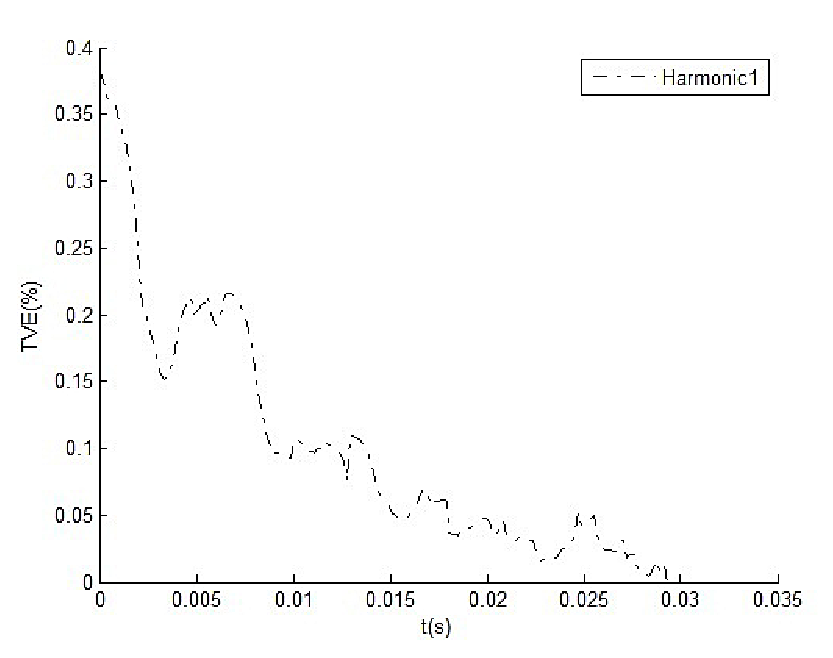
\includegraphics[scale=0.67]{BLMS_Figures/StaticTestResult}
\caption{Static test results using a quarter cycle data window}
\label{StaticTestResult}
\end{center}
\end{figure}

\subsection{Noise Test}
The inherent noise rejection capability of the algorithm is investigated by this test. The signal model for the static test is used. Each run is for $2$ cycles. We observe that even under worst case condition of $30$ dB signal to noise ratio, if the data window used is equal to one cycle the algorithm can give still a very low TVE.  For different noise levels, the TVE for the B-LMS and RWT is evaluated and compared as shown in Table \ref{NoiseTestResultsTable}.

\begin{table}[H] 
\renewcommand{\arraystretch}{1.3}
\caption{Noise test results} \label{NoiseTestResultsTable}
\centering
\begin{tabular}{c|c|c|c}
\hline
Noise				&	Data block	  &  B-LMS     &  RWT	  \\
Level			    &  length $(l_s)$ &   TVE	   &  TVE	  \\
(SNR)			    &				  &   $ \%$    &  $ \%$   \\
\hline\hline
			 & 	$ 0.25$		&	$0.2295$		&	$0.36$ \\
\cline{2-4}
$0.1\%(60dB)$&	$ 0.5$		&	$0.0197$		&	$0.12$ \\
\cline{2-4}
			 &	$ 1.0$		&	$0.00007$		&	$0.036$ \\
\hline
			 &	$ 0.25$		&	$0.3582$		&	$0.94$ \\
\cline{2-4}
$0.32\%(50dB)$&	$ 0.5$		&	$0.1137$		&	$0.40$ \\
\cline{2-4}
			 &	$ 1.0$		&	$0.00057$		&	$0.064$ \\
\hline
			 &	$ 0.25$		&	$1.5025$		&	$1.60$ \\
\cline{2-4}
$1\%(40dB)$  &	$ 0.5$	    &	$0.3984$		&	$1.08$ \\
\cline{2-4}
			 &	$ 1.0$		&	$0.0023$		&	$0.26$ \\
\hline
			 &	$ 0.25$		&	$8.8573$		&	$2.73$ \\
\cline{2-4}
$3.2\%(30dB)$&	$ 0.5$		&	$1.3426$		&	$1.59$ \\
\cline{2-4}
			 &	$ 1.0$		&	$0.0086$		&	$0.68$ \\
\hline
\end{tabular}
\end{table}


\subsection{Dynamic Step and Ramp Change Test}
To evaluate the dynamic response when exposed to an abrupt signal change, a positive step followed by a reverse step back to the starting value under various conditions is applied to the amplitude and phase angle of a sinusoidal signal, respectively. Studies indicate that under both types of steps the algorithm shows similar dynamic behavior. Here we used a block size of $12$ samples since only two weights are to be computed (i.e. $.1$ cycle). The results of the amplitude step ($10\%$ of normal value) and phase step ($\pi/18$ rad), are presented by Figs. \ref{DynamicResAmpStep}- \ref{DynamicResAmpStepFiltered}, respectively without any iterations used for blocks of data. The steps occur at $0.02$ and $0.06$ s. One can observe that the outputs track the changes in the inputs extremely fast. It took $1.39$ ms and $1.94$ ms to fully track the amplitude step change and $1.67$ ms and $1.81$ ms to track phase step change that occurred at two different times respectively. To investigate the effect of prefiltering on the algorithm dynamic performance, a third order Butterworth low-pass filter with a cutoff frequency of $320$ Hz is used to process the input signals. Fig. \ref{DynamicResAmpStepFiltered} shows the result of amplitude step test. Compared to Fig. \ref{DynamicResAmpStep}, which shows the transient behavior without signal prefiltering, one can see that the low pass just slows the response from $3$ to $5$ ms with no significant overshoot and undershoot and it is still less complex than the RWT-based method \cite{Ren2011} that takes about a quarter cycle of fundamental component time period, DFT-based methods \cite{Benmouyal1989} -\cite{Sidhu1998} and faster than instantaneous sample-based methods \cite{Kusljevic2010}, \cite{Lopez2008} that require full cycle of fundamental component about $16.66$ ms. A dynamic amplitude response for a ramp change is also done. The ramp occurs at $0.02$ s and continues to steadily increase till $0.06$ s then it drops back to the original value as shown in Fig \ref{DynamicRampTest}. It is clear that the algorithm tracks the constant changes steadily and the drop is tracked just in $1.67$ ms. The performance of the algorithm showed similar result in phase test.

\begin{figure}[H]
\begin{center}
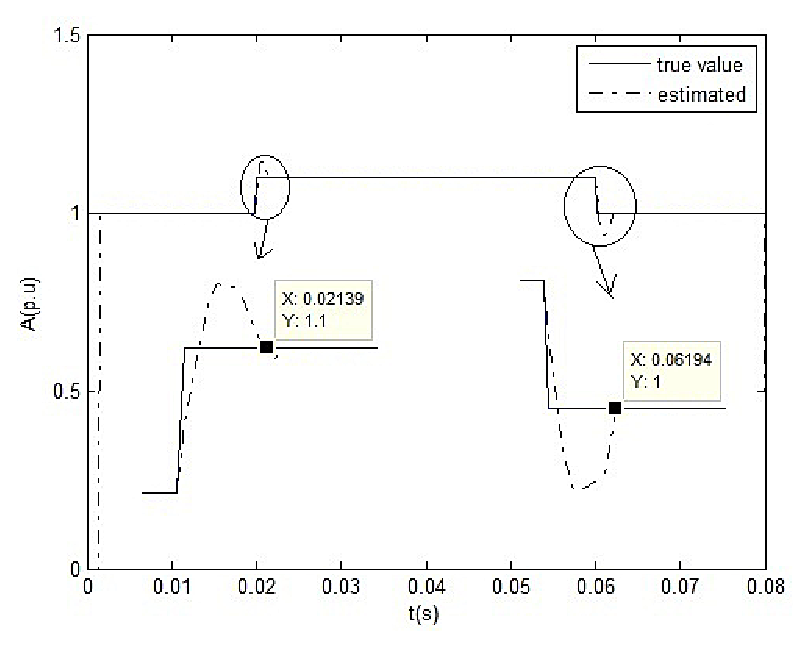
\includegraphics[scale=0.74]{BLMS_Figures/DynamicResAmpStep}
\caption{Dynamic response for the amplitude step}
\label{DynamicResAmpStep}
\end{center}
\end{figure}

\begin{figure}[H]
\begin{center}
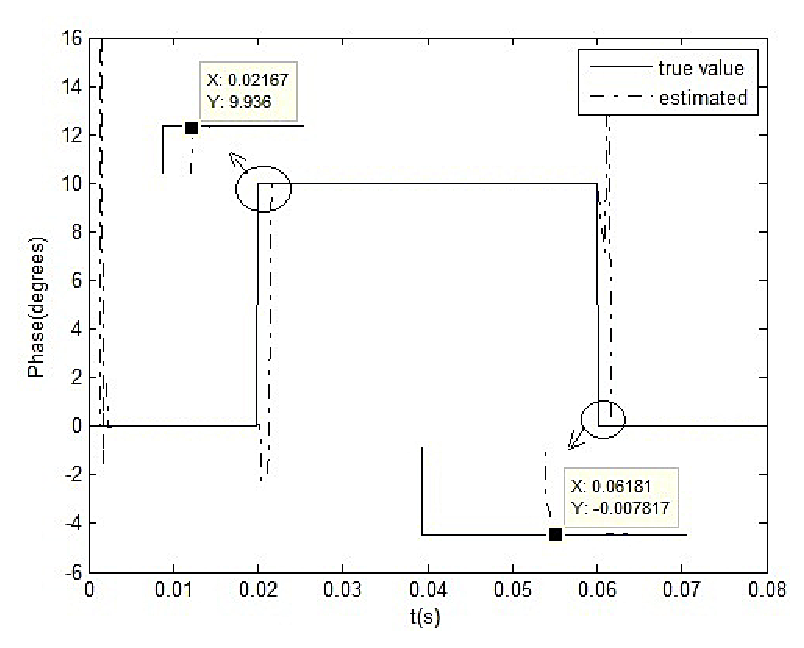
\includegraphics[scale=0.74]{BLMS_Figures/DynamicResPhaseStep}
\caption{Dynamic response for the phase step}
\label{DynamicResPhaseStep}
\end{center}
\end{figure}

\begin{figure}[H]
\begin{center}
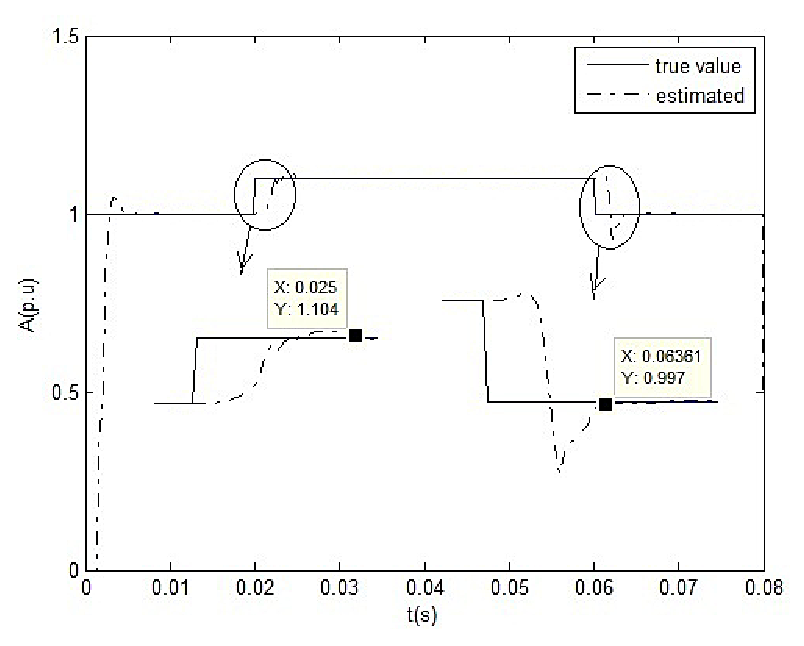
\includegraphics[scale=0.75]{BLMS_Figures/DynamicResAmpStepFiltered}
\caption{Dynamic response for the with amplitude step with prefiltering.}
\label{DynamicResAmpStepFiltered}
\end{center}
\end{figure}

\begin{figure}[H]
\begin{center}
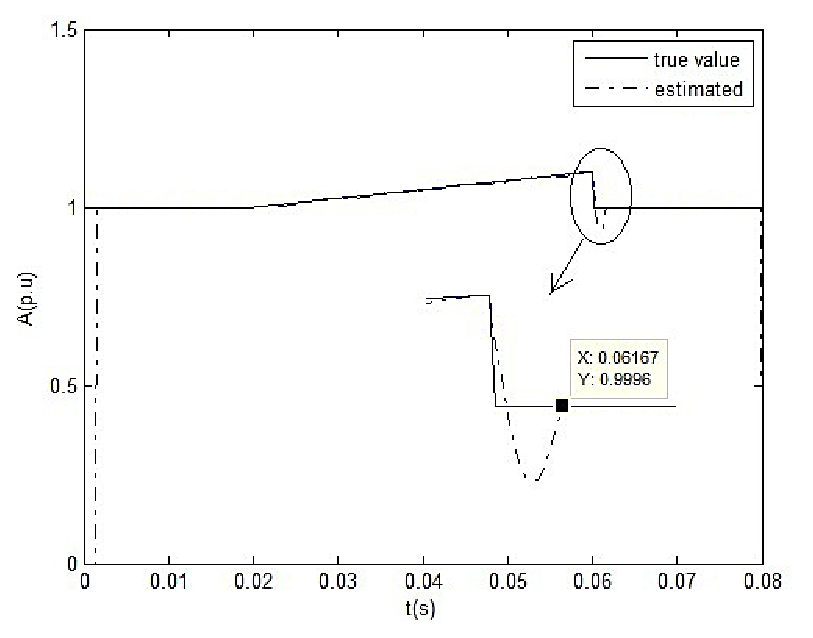
\includegraphics[scale=0.75]{BLMS_Figures/DynamicRampTest}
\caption{Dynamic response for the amplitude ramp change}
\label{DynamicRampTest}
\end{center}
\end{figure}

\subsection{Transient Test}
A synthetic three phase waveforms based on the model in \eqref{eq:fund_Harmonic_Model_DC}, is used for testing the performance for eliminating the decaying dc offset. A change in the amplitude is done beginning $0.05$ s, similar to a three-phase fault generated in real system. Fig. \ref{TransientTest} shows the current waveform of Phase A used for simulation. One can see that the signal is contaminated with decaying dc component and high frequency noise is present at the beginning and during the fault. The third order Butterworth low pass filter with a cutoff frequency of $320$ Hz is used to attenuate the high-frequency components. Parameters estimation for steady state (twenty cycles after the fault occurs) is used as a reference to measure the TVEs. As shown in the Table \ref{DecayingDCTable}, the results are compared with the conventional full-cycle DFT(FCDFT), half-cycle DFT(HCDFT or STFT), least error square(LES), hybrid method [21], and simplified algorithm (SIMS) in \cite{Gou2003}. In the Table \ref{DecayingDCTable}, $t_s$ is the time(in cycles) when the TVEs are measured. For high accuracy, the algorithm was adjusted to a full cycle window span. The results show that the accuracy is clearly comparable to those of LES. But it is superior in terms of convergence characteristics to LES, SIM3, and HM using first order optimization (Jacobian) technique.

\begin{figure}[H]
\begin{center}
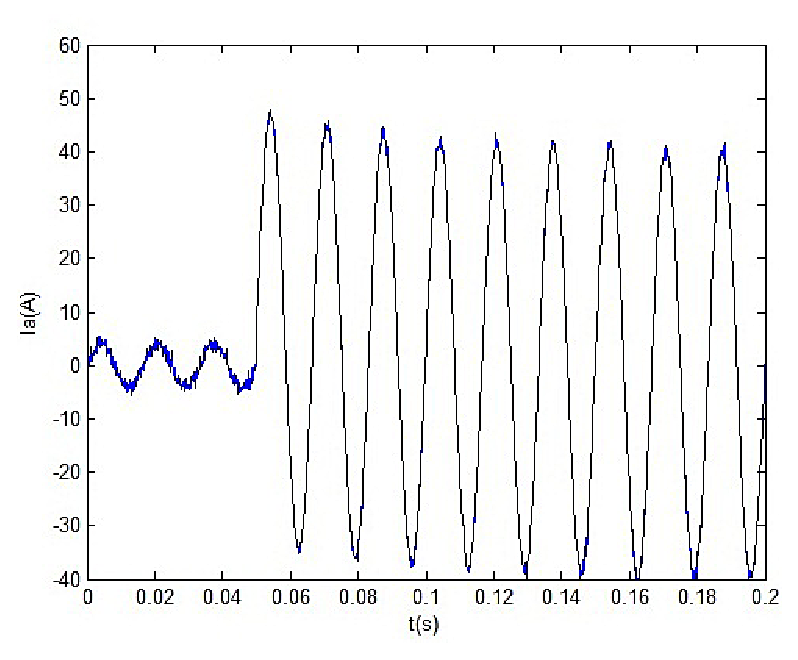
\includegraphics[scale=.8]{BLMS_Figures/TransientTest}
\caption{Simulated Current $I_A$ waveform for transient test}
\label{TransientTest}
\end{center}
\end{figure}

\begin{table}[H] 
\renewcommand{\arraystretch}{1.3}
\caption{Test Results for decaying dc offset} \label{DecayingDCTable}
\centering
\begin{tabular}{c|c|c|c|c}
\hline
Algorithm &	ts(cycle)&	IA      &  IB 	    & IC 		\\
		  &          &TVE$(\%)$ & TVE$(\%)$ & TVE$(\%)$ \\
\hline\hline 
FCDFT	 &	5		&$0.9474$	&$0.9587$	&$0.9559$	\\
\hline
HCDFT	&	12.5	&$1.0148$	&$1.0196$	&$1.0158$	\\
\hline
LES	&	1.0		&$0.1036$	&$0.1073$	&$0.1058$	\\
\hline
SIM3	&	1.0		&$0.1285$	&$0.1089$	&$0.1153$	\\
\hline
HM		&   1.0		&$0.1273$	&$0.1168$	&$0.1132$	\\
\hline
B-LMS	&	1.0		&$0.1023$	&$0.1034$	&$0.1046$	\\
\hline
\end{tabular}
\end{table}


\section{Conclusions} \label{BLMSConclusions}

The chapter introduces a new adaptive filtering approach to solve the problem of phasor estimation when the frequencies of components are known. The algorithm features very fast response and high accuracy over varied conditions in noise. It uses less than a quarter cycle of fundamental component signal to estimate amplitude and phase for a signal contaminated with harmonics or interharmonics. A high frequency resolution could be achieved using this model based technique by appropriately modeling weights. The decaying dc component can be completely removed using this technique. The performance of the algorithm is evaluated under a variety of conditions that includes static test, noise test, dynamic test and transient test. Comparison with other techniques demonstrates the advantage of using this approach. The computational burden is minimal when compared to non-linear or second order methods or wavelet based methods; accuracy is high and response is very rapid to satisfy time-critical demand of the real time applications in power system. This model can be easily adapted to drifts in nominal frequency when it is known.

This is one of the most efficient time domain methods. So only accurate information of amplitude and phase can be extracted using this method, not the frequency information. If one method tries to extract both time and frequency domain information from a signal, for instance RWT, its complexity goes high, its response time is reduced, its accuracy is usually limited due to a trade-off. In high noise environment difficulty increases further. But a combination of two best methods, each extracting time and frequency domain information separately, would easily be better. Once this B-LMS technique is combined with a fast frequency domain method, whose computations can precede this algorithm, then it can be used for frequency distorted signals too. In power systems, as is well known, frequency is much more tightly regulated parameter than amplitude and phase of various signal components, where this technique can be productively employed. Further research is required to estimate the nominal frequencies and its drift using some efficient approach and in combination with this filtering algorithm.



\chapter{FREQUENCY ESTIMATION FROM NONUNIFORM SAMPLES}\label{FreqEst}

\epigraph{ Bone of our bone, and flesh of our flesh, and 
blood of our blood, \\
are there half-brutish prehistoric brothers and sisters.\\
 Gridled about with the immense darkness of \\
 this  mysterious universe even as we are,\\
 they were born and died, suffered and struggled.\\
 Given over to fearful crime and passion,\\
 plunged in the blackest ignorance, \\
 preyed upon by hideous and grotesque delusions,\\
 yet steadfastly serving the profoundest of ideals in their fixed faith\\
 that existence in any form is better than non-existence, they ever \\
 rescued triumphantly from the jaws of ever-imminent destruction\\
 the torch of life which, thanks to them, now lights the world for us. \\
 How small indeed, seem individual distinctions when \\
 we look back on these overwhelming numbers of human beings\\
  panting and straining under the pressure of that vital want !\\
  And how inessential in the eyes of God must be\\
   the small surplus of the individual's merit,\\
   swamped as it is in the vast ocean of the common merit of mankind,\\
   dumbly and undauntedly doing the fundamental duty,\\
   and living the heroic life !\\
   We grow humble and reverent \\ as we contemplate the prodigious spectacle. }
{\itshape William James, in Human Immortality, $1898$.}

Sinusoid signals with multiple frequencies appear in various systems and their frequencies may carry some important features. Frequency estimation from their discrete samples is one of the fundamental
problems  and many frequency estimators have been proposed for uniform sampling setting \footnote{Part of the material in this section is reprinted from ``Frequency estimation of sinusoids from nonuniform samples" by Syed Alam Abbas, Qiyu Sun, and Hassan Foroosh, Signal Processing Elsevier, vol. 129, pp. 67-81, 27 May 2016 \copyright 2016 Elsevier, with permission from Elsevier.}.

In this chapter, frequency estimators based on adaptive notch filtering are proposed for nonuniform sampling setting. Most signal processing algorithms are designed to handle uniformly sampled signals. Real world signals usually exist in its analog form, they are converted to digital form by sampling at equal intervals. If $y_{\text{analog}}(t)$ is a \emph{continuous time signal} (analog), its samples give a discrete/digital time signal:
\begin{equation}
y_{\text{digital}}(n) = y_{\text{analog}}(n\Delta T), n = 0,\pm 1,\pm 2, \cdots
\end{equation}
The \emph{sampling interval} is $\Delta T$. Often this interval is normalized to $\Delta T = 1$, by a simple rescaling of the time variable.

We observe that some dynamic systems designed for continuous time signals associated with adaptive notch filters can be solved in nonuniformly
sampled time steps with high accuracy. This leads us to propose a digital adaptive notch filtering method to estimate frequency of a sinusoidal signal with single frequency from its nonuniform samples. The proposed method exhibits convergent and robust frequency estimation in the presence of random sampling noises, and its variance is comparable to the Cramer-Rao lower bound in the presence of additive white noise. The above method designed for single frequency estimation could track abrupt single frequency change of an input signal, but it is not applicable directly for multiple frequency estimation. Our simulations show the proposed estimators have robust performance for sinusoidal signals with multiple distinct frequencies, and they can be used to separate two very close frequencies of an input signal in a highly noisy sampling environment.


\section{Introduction}
Consider a mixture of sinusoidal signals, whose $k$-th component has amplitude $A_k$, frequency $\theta_k$ and  phase $\phi_k, 1\le k\le K$,
\begin{equation}\label{multiSinusoids1}
y(t)=\sum\limits_{k=1}^{K} A_k \sin(\theta_k t+\phi_k).
\end{equation}
Such  sinusoidal signals are encountered in  % various telecommunications systems,
    active noise and vibration control, wireless communications, audio, radar and sonar signal processing \cite{regalia91, fuller96, Klapuri03, simone}. %,  Tong10}). % Jacobson08,
In telecommunication systems, the  frequencies $\theta_k, 1\le k\le K$,
 contain carrier's phase information necessary for synchronization of demodulators or other components of a receiver system.
 % \cite{regalia91}.


The estimation problem  of
frequencies $\theta_k, 1\le k\le K$, of the signal $y$
is a fundamental problem in systems theory with many  applications.
It has been  intensively studied in  signal processing, instrumentation and measurements, and control theory.
Many frequency estimators have been proposed, including adaptive notch filtering, time frequency representation, phase locked loop, eigensubspace tracking, extended Kalman filtering, internal model method etc, see  \cite{%Tong10,
Hsieh93, Badeau06, zhangbrown06, karimi11} and references therein.


Most of existing estimators are derived for uniformly sampled  data
$y(n\triangle T), n\ge 0$, with uniform sampling frequency $1/\triangle T$,
and often only for a single  % fixed
frequency, i.e., $K=1$.
In this paper, we consider
multiple frequency estimation problem
of the signal $y$ %in \eqref{multiSinusoids1}
from its
nonuniform samples,
\begin{equation}\label{multiSinusoids2}
z_n = y(T_n)+ w_n, \ n\ge 0,
\end{equation}
corrupted by  additive noises $w_n$,
where $T_n, n\ge 0$, are  sampling times.

Nonuniform sampling  arises in many  applications such as computer graphics, frequency scanning interferometry,
magnetic resonance imaging, % (MRI), % (MRI),
computer tomography  % (CT)
scans and Radon imaging
 \cite{dutt93, stoica97,stoica00,  Marvasti01, Frida07, Maciejewski09}. 
Uniform sampling is well studied and it has been widely used in engineering applications. However in some applications,  
  nonuniform sampling is necessary and  it has better performance.  For instance, in antialiasing in computer graphics \cite{Cook1986}, better results can be obtained with random sampling instead of uniform sampling. The sampling operation  could be costly, and a low number of samples (but not necessarily uniform) is more desirable. For instance, in frequency scanning interferometry,  the sampling effort is measured by the acquisition time at a given point, and the optimal sampling scheme is  usually nonuniform \cite{Stefan2009}.
  Nonuniformly sampled data are harder to analyze and the related methods, even for a ``simple" task of obtaining the
  discrete nonuniform Fourier transform,
  are much more difficult and often iterative \cite{dutt93, %Aboy04,
  holland09}.
   Several statistical frequency estimators (based on maximum likelihood estimation and filter banks) from nonuniformly sampled data
   have been proposed in  the literature \cite{stoica00, % Hossein, James95,
    Gansman, Yonina00,Johansson02,Ryan04, tarcznski04, Dongdong}.
For  nonuniform sampling problems in signal processing, the reader may refer to \cite{unserieee,  akramsiam,  sunsiam}.  %Jesse10,
% Babu12}. %, Duarte12, Marvasti12,  Dinesh13}.
%{\color{blue} Do we need so many FRI references ? Can we remove some ?}

 In many applications of signal processing, it is desirable to eliminate or extract sine waves from observed data or to estimate their unknown frequencies. Since the frequencies often vary with time, it is useful to apply adaptive notch filters (ANF's) that adapt their notch frequencies as a function of the observed time series,  %. The subject of notch filtering has been widely studied,
 see  \cite{Nehorai1994}, \cite{Marina1995} and references therein. The ANF method is
one of most suitable techniques to separate sinusoidal components of unknown frequencies  buried in noise, and/or retrieve such periodic components  (\cite{ hsuortegadamm99,  marino02, xia02, mojiri04, hou05, mojiri07, mojiri07b}).
      %when noisy uniform samples of the sinusoid signal is available.
   It is robust in the presence of sampling noise and it  is capable of changing the notch frequency accordingly.
   % by tracking the frequency variations of the input signal.
   Various architectures   have been proposed for the construction of adaptive notch filters, see
   for instance
   \cite{ regalia91, regalia95, debrunner00, limzouzheng05, cousseau07, tanjiang09, regalia10}.

 Frequency estimation problem using ANF is modeled as a nonlinear system identification of a dynamic system either in continuous time (CT) \cite{regalia91} or in discrete time (DT) \cite{hsuortegadamm99}. The CT model systems are native to the physical world, they have a built-in capability to cope with the nonuniformly sampled signal,
and they offers certain advantages over purely DT model systems \cite{Rao06, Garnier08}.
Compared to the DT model, % may yield undesirable sensitivity problems at high sampling rates, whereas
direct estimation of CT models is usually stable, accurate and free from undesirable sensitivity problems, particularly at high
sampling rates.  The frequency estimator developed in this paper is based on ANFs, which are governed by some CT dynamic systems \cite{hsuortegadamm99, marino02, xia02, mojiri04, hou05, mojiri07, mojiri07b, bodsondouglas97, dammhsuortega98, hou13}. We mainly
 focus on a particular ANF governed by the following dynamic system,
 % \cite{hsuortegadamm99},
  \begin{equation} \label{Hsu_ANF}
  \left\{
\begin{array}{l}
D{x_1} = x_2   \\
D{x_2} = -2\xi \theta x_2 - {\theta}^2x_1 + {\theta}^2y  \\
D{\theta} = -\gamma ({\theta}^2y - 2\xi \theta x_2)x_1,
\end{array}
\right.\end{equation}
where  $D$ represents the derivative with respect to time $t$, $x_1,x_2,\theta$ are  states of the system, $y$ is the excitation sinusoidal input with single frequency $\theta_0$ (i.e., $K=1$ in \eqref{multiSinusoids1}), $\xi$ is the notch depth, and $\gamma$ is the adaptation speed.    % (\cite{hsuortegadamm99, marino02, xia02, mojiri04, hou05, mojiri07, mojiri07b,   bodsondouglas97, dammhsuortega98, hou13}).
 The above system of nonlinear ordinary differential equations (ODE)
 has good noise rejection capability. It was proposed by Regalia in \cite{regalia91} as a DT filter, it was later adapted by Bodson and  Douglas \cite{bodsondouglas97} for a CT system, and finally a modified version was proposed by Hsu, Ortega and Damm \cite{hsuortegadamm99}.
 We have chosen this dynamic system due to its superior performance compared to the other systems that can be used with a similar discretization procedure, see Section \ref{extension.subsection} for performance comparison. %simulation confirmation.
%The continuous version of the ANF structure proposed by  Hsu,  Ortega and Damm
%is  a scaled
%and normalized
%  formulation of Regalia's ANF  method %\eqref{RegaliaANF}


 The main difficulty in handling CT dynamic systems directly is the problem of evaluating
  derivatives of the input signal (with unknown parameters) from its nonuniform samples numerically, the numerical differentiation process in a highly noisy environment is usually unstable and impractical \cite{Tseng01, Papoulis77,Cheung85}.
  In this chapter, we propose a Taylor-like approximation of the dynamic system \eqref{Hsu_ANF}
   that is robust to noise and achieves high accuracy. Based on the above approximation,
 we introduce an ANF  method \eqref{mainalgorithm}  to estimate the frequency of a sinusoidal signal from its
 nonuniform samples. The proposed discrete ANF method reconciles the merits of CT models while restricting itself to operate directly on the DT data.







%   The lattice-based DT filter was first proposed by Regalia (\cite{regalia91, regalia95}),
%   and many designs have been advanced by exploiting either constrained poles and zeros through direct coefficient scaling (\cite{limzouzheng05,tanjiang09}), or through all-pass decompositions (\cite{regalia95,debrunner00,cousseau07,regalia10}).
%   %, with latter being more efficient \cite{regalia95}.
%   % over the years in digital filters
%   %\cite{regalia95,regalia10}
%   The lattice-based DT filter in \cite{regalia91}
%   was  adapted for CT in \cite{bodsondouglas97}, which
% is described by  nonlinear dynamic systems in continuous domain, see
% see \cite{karimi11, hsuortegadamm99,  marino02, xia02, mojiri04,   hou05, mojiri07, mojiri07b, dammhsuortega98, hou13}. In this paper,






%The frequency estimation problem could be modeled as a nonlinear  dynamic system.
%The adaptive notch filtering (ANF) is  one of most suitable
%   techniques to separate sinusoidal components of unknown frequencies
%   (\cite{karimi11, hsuortegadamm99,  marino02, xia02, mojiri04,   hou05, mojiri07, mojiri07b}).
%      %when noisy uniform samples of the sinusoid signal is available.
%   It is robust in the presence of sampling noise and it  is capable of changing the notch frequency accordingly.
%   % by tracking the frequency variations of the input signal.
%   Various architectures have been proposed for the construction of adaptive notch filters, see
%   for instance
%   \cite{ regalia91, regalia95, debrunner00, limzouzheng05, cousseau07, tanjiang09, regalia10}.





%\indent One broad way to classify the methods is through their model description. The lattice-based discrete-time (DT) filter that was first proposed by Regalia \cite{regalia91} was later adapted for continuous time (CT) in \cite{bodsondouglas97}, which is simply described by a set of non-linear first order differential equations. Many designs have been advanced over the years in digital filters \cite{regalia95,regalia10} exploiting either constrained poles and zeros through direct coefficient scaling \cite{limzouzheng05,tanjiang09}, or through all-pass decompositions \cite{regalia95,debrunner00,cousseau07,regalia10}, with latter being more efficient \cite{regalia95}. For CT versions there has been many advances \cite{dammhsuortega98}--\cite{hou13}. These studies show that methods used in communities of signal processing and control have barely influenced each other. Perhaps the different goals cause this poor interaction. In signal processing the focus is signal analysis in noisy measurements mostly using DT models, while in adaptive control it is estimating sinusoids to ensure asymptotic stability mostly using CT models. % \\


 This paper is organized as follows. Section \ref{sec:singlef} discusses a Taylor-like approximation technique to solve the system \eqref{Hsu_ANF}  and  a  frequency estimation of the unknown input signal with single frequency.
We propose the frequency estimator \eqref{mainalgorithm}, perform the local stability analysis,
and  study its convergence, noise characteristics,  statistical properties, and comparison to the conventional
  ODE solver for the dynamic systems associated with the ANF methods. We also perform a comparison of our method with a state of the art discrete ANF \cite{tanjiang09}.  %along with comparison simulation with a
 % of %competitive
%  discrete ANF \cite{tanjiang09}.
% All design steps, such as  are compared the complexity of the proposed scheme against any other technique.
Section \ref{sec:mult} describes extensions
   of the single frequency estimator \eqref{mainalgorithm}
      to multiple frequency estimations with two configurations,
      the cascade ANF method and the prefiltering ANF method.
 The two proposed multiple frequency estimators have  robust performance for  sinusoidal signals with  multiple distinct frequencies or related harmonic frequencies.
Most of the known frequency estimators have poor performance
when input signal has two very close frequencies in a highly noisy environment, a pathological case where the estimation error is related to both the difference in the frequency and the noise level, see \cite{Shahram05} and references therein.
Our simulation indicates that the cascade ANF method
has sound performance even in the separation of very close frequencies of the input signal in a highly noisy sampling environment.
We close the paper with concluding remarks in Section \ref{sec:conclusion}.



% We observe that some dynamic systems associated with ANFs can
%  be solved using nonuniformly-spaced time steps  with high accuracy.
%  So
%  we propose a Taylor-like approximation of the dynamic system \eqref{Hsu_ANF},
% and then we introduce  discretized adaptive notch filtering method \eqref{mainalgorithm} of order $m\le 4$
%  to estimate the frequency of  a sinusoid signal with single frequency.
%In  Section \ref{sfe.section}, we demonstrate convergence of the discretized adaptive notch filtering method \eqref{mainalgorithm}
% for middle-range frequencies,
%show its ability to track  frequency change  when  the input signal has time-varying frequencies,
% %compare its performance with the standard Runge-Kutta method on approximation,
% combine it with  heterodyning for high frequency estimation,
% and compare its variance with the Cramer-Rao low bound in the presence of random sampling noises.


%\indent Frequency estimation problem can be also modeled as a nonlinear system identification of a dynamic system. It is a well-established field and deals with the problem of determining mathematical models of dynamical, CT systems using measured and sampled data. The dynamical systems encountered in the physical world are native to the continuous domain, which offer certain advantages over purely discrete time (DT) systems \cite{Rao06}. There are fundamentally two different time-domain approaches to the problem obtaining a CT model of a natural CT system from its sampled data \cite{Garnier08}:
%\begin{itemize}
%\item {\em The indirect approach} which involves identification of a DT model in an `all-digital setting' and transformation into CT form.
%\item {\em The direct approach} in which the CT model is identified straightaway. In this direct approach, the model remains in its original CT form.
%\end{itemize}
%\noindent
%There are a number of advantages in using direct CT models \cite{Garnier08}, over its discretized DT models (indirect approach), e.g. CT models are a more natural representation of the underlying phenomena, discretisation may render the CT models with non-minimum phase \cite{Sinha91}, and finally the issue that discretisation gives rise to undesirable sensitivity problems at high sampling rates, whereas direct estimation of CT models is free from all these problems and it assures stable and more accurate models, particularly with rapidly sampled data. On the other hand the main difficulty in handling directly the CT models is due to the presence of the derivative operator associated with the input and output signals. Any attempt at directly realizing it either by numerical computation or signal processing through a differentiator will result in amplification of noise \cite{Papoulis77,Cheung85}, hence it is challenging. In this paper we show the solution of a CT model system well designed for frequency estimation via the direct approach that is robust to noise and also achieves high accuracy.
%The main advantage of identifying the CT models directly from sampled data is that it is independent of the sampling period, and hence it has a built-in capability to cope with the non-uniformly sampled signal. %\\
%It is worth noting that a simple and direct DT frequency estimator as  using non-uniform samples and a model of the deterministic CT differential system has not been proposed. \\

%\indent However the scheme for finding the filter equations in discrete time, for either the ANF structures or the adaptive observer based differential systems for use in spectral estimation is the same as described in Fig \ref{ODESolverInDiscreteTime.fig}. In particular, the higher order derivatives for Mojiri ANF structure \eqref{Mojiri_ANF} should have similar terms as \eqref{firstderivative}-\eqref{forthderivative} except the scaling change. So using our direct discrete method such changes in the design of differential equations can easily be implemented with just few slight modifications to the derivatives. Or any dedicated designed similar differential system for spectral analysis can be used in a purely discrete time setting using the proposed model for a specific application. In the following simulations we compare the solution of the proposed method of solving ODEs with the solution obtained from the Runge-Kutta method (using the Matlab $ode45$ implementation) for Hsu ANF structure. \\
%
%\indent Compared to the continuous domain filters, such as PLL based frequency estimator, these structures based on the differential systems do not use a voltage controlled oscillator (VCO), and hence are simple and direct in thier digital implementation using \eqref{generalxtapproximation}. The other structures like continuous ANF use multiple integrators for which the sampling rate must be relatively higher since they are implemented using analog components. Since the middle of the last century when CT model started to emerge, there has been overwhelming developments in DT methods for some time mainly to the `go completely digital' trend that was spurred by parallel developments in digital computers \cite{Rao06}. Our method seeks to reconcile the merits of CT models while restricting itself to operate directly on DT data.



%An ideal notch filter has unit gain at all frequencies except at
%notch frequency where its gain is zero. We then guess that
%the  discretized adaptive notch filtering method \eqref{mainalgorithm}
%designed for single frequency estimation could be applicable for multiple frequency estimation
%if  initial frequencies are  selected to be not far away from true frequencies.
%For input signal with multiple frequencies, the phenomenon is observed that
%the discretized  system \eqref{mainalgorithm} does converge when notch depth and adaption speed are appropriated chosen, but it may converge to the dominant frequency of the input signal.
%So in Section \ref{mfe.section}, we propose two  configurations,  cascade ANF and prefiltering ANF,
%for multiple frequency estimation. Our simulations show that those two frequency estimators have  robust performance for  sinusoid signals with  multiple separate frequencies and  harmonic frequencies.
%Most of known frequency estimations has poor performance
%when input signal has two very close frequencies, see \cite{Shahram05} and references therein.
%Our simulation indicates that the cascade ANF method
%has sound performance on separation of very close frequencies of the input signal in highly noisy sampling environment.
%



%\indent The remaining of this paper is organized as follows: Section \ref{sec:singlef} discusses single frequency estimation using an approximation technique to solve a set of ODE using fixed time steps, including the supporting mathematical theory, the study of convergence, the statistical properties, and the stability analysis.

% Section \ref{sec:comp} discusses the performance comparison of the proposed discrete solver with the conventional ODE solvers, along with a study of different structures and comparison of solutions obtained. It also discusses a solution to extend its effective spectral range of estimation. Section \ref{sec:mult} describes the extension to multiple frequencies, including three configurations and simulations with specific examples of sum of two components, discussion of a pathological case with two very low frequencies in the presence of high noise, and finally the case of multiple harmonics and arbitrary number of components. We close the paper with concluding remarks in section \ref{sec:conclusion}. \\

%Notation: We have used Euler notation here for expressing derivatives $D^n$ instead of $D^n_t$ to denote the $n^{th}$ derivative with respect to time $t$.

Notation: We use Euler notation for expressing derivatives, $D^n$ instead of $D^n_t$ to denote the $n^{\rm th}$ derivative with respect to time $t$.


\section{Single frequency estimation} \label{sec:singlef}
\label{sfe.section}


%In this section, we propose a  single frequency estimation
%of a sinusoid  input  signal from its nonuniform samples.

 Consider a sinusoidal input
 \begin{equation}\label{sinusoid.def}
 y(t) = A \sin(\theta_0 t + \phi),\end{equation}
 where $A, \theta_0, \phi$ are its
amplitude, frequency, and phase, respectively.
%$A$, frequency $\theta$  and phase $\phi$,
In the first subsection, we propose  a discrete ANF method to
estimate frequency $\theta_0$ of the sinusoid  signal  $y$ %in \eqref{sinusoid.def}
 from its nonuniform samples,
%In this section, we propose a discrete ANF
%method %\eqref{mainalgorithm}
%to
%estimate frequency $\theta_0$ of the  input signal
%$y$ %in \eqref{sinusoid.def}
% from its  nonuniform samples
\begin{equation}\label{singularfrequencydata}
z_n=y(T_n)+w_n,\ \  n\ge 0,\end{equation}
 corrupted by additive noise  $w_n$
at sampling times $T_n, n\ge 0$.
Then in the next four subsections, we  discuss local stability,  convergence, approximation error, statistical characterization, and extensions of the proposed  ANF method. 
We also compare the performance of our approach \eqref{mainalgorithm} with some of the existing ANF methods for estimating frequency in Section \ref{convergence.subsection} and Section \ref{extension.subsection}.

%In the following sections, we demonstrate convergence of the
%discrete ANF method  \eqref{mainalgorithm} using nonuniform sampling data of
%sinusoids in different settings. We begin our discussion using two simple examples with different frequencies to be estimated from nonuniform data. Then we fix the input signal frequency and study the effects of change in the amplitude, keeping all other parameters constant, in terms of both the speed and accuracy of convergence of our method. We do a numerical comparison with the standard solution obtained from the Runge-Kutta (R-K) method  \cite{burden10}. Next we show the choice of the approximation order depends on the sampling rate and the input signal frequency, the higher the order the better is the accuracy we achieve in the frequency estimation and there is a range of frequencies that can be effectively estimated with a particular order, we also briefly discuss the dynamic convergence in case of frequency hops and the accuracy achieved with different orders. The next part extends the solution for high frequencies that cannot be directly estimated using the proposed solution. We follow it with the statistical characterization of the proposed frequency estimator by comparing it with the Cramer-Rao lower bound, we then fix the amplitude and frequency and vary the SNR to study its noise characteristics. Finally we generalize our procedure and show how it can be used to solve other differential systems proposed in the literature for frequency estimation.




%\subsection{Preliminaries}
%
%
% An ANF is capable of changing its notch frequency by tracking frequency variations of the input signal. Various architectures have been proposed for the construction of an ANF. In this paper, we  mainly focus on a particular ANF structure, which originated in \cite{regalia91}, later adapted for CT in \cite{bodsondouglas97}, and finally  modified by  Hsu,  Ortega and Damm in \cite{hsuortegadamm99},
%%The continuous version of the ANF structure proposed by  Hsu,  Ortega and Damm
%%is  a scaled
%%and normalized
%%  formulation of Regalia's ANF  method %\eqref{RegaliaANF}
%  \begin{equation} \label{Hsu_ANF2}
%  \left\{
%\begin{array}{l}
%D{x_1} = x_2   \\
%D{x_2} = -2\xi \theta x_2 - {\theta}^2x_1 + {\theta}^2y  \\
%D{\theta} = -\gamma ({\theta}^2y - 2\xi \theta x_2)x_1,
%\end{array}
%\right.\end{equation}
%where $x_1,x_2,\theta$ are  states of the system, $y$ is the excitation sinusoidal input of unknown frequency $\theta_0$, $\xi$ is the notch depth, and $\gamma$ is the adaptation speed.







   %\frac{A^2\gamma}{4\xi} < 1.$$

%\indent Now the problem of the frequency estimation reduces to solving the above dynamical system, given a set of non-uniformly sampled data for the sinusoidal input, $y$ and initial conditions. We use the \emph{Cauchy-Kowalevskaya} theorem \cite{evans98}, we only require that the non-linearity present in the ODE be analytic in $t$ and its states.\\ \\
%\emph{Theorem 1}:\emph{ ({Cauchy-Kowalevskaya} theorem for ODEs) \\ Let $F: R \times R^n \rightarrow R^n$ be a real analytic funtion in the domain $[-t_0,t_0] \times B_{\delta_0}(X_0)$, where $B_{\delta_0}(X_0)$ is an open ball in $R^n$ centered at $X_0$ with some radius $\delta _0 > 0$ and $t_0 > 0$. Let $X(t,X_0)$ be a unique solution for $t\in [-t_0, t_0]$ of the initial value problem,
%\begin{eqnarray} \label{CauchyKowalevskaya}
%DX = F(t,X),   \nonumber \\
%X(0) = X_0
%\end{eqnarray}
%Then $X(t,X_0)$ is also real analytic  function of $t$ near $t=0$. That is, there exists $\tau \in (0,t_0)$ such that : $X: [-\tau , \tau ] \rightarrow R^n$ is a real analytic function. } \\
%\indent See \cite{evans98} and \cite{tutschke89} for details and proof of this theorem. The theorem in simple terms basically guarantees that for all analytic systems, the solution obtained will also be analytic. Thus we can directly use time derivatives at each differential equation level to advance the solution using given initial conditions without necessity of computing any partial derivatives between the states.  \\

\subsection{The proposed method}
\label{danf.subsection}




%In this subsection, we propose  a discrete ANF method to
%estimate frequency  of a sinusoid  signal in \eqref{sinusoid.def} from its nonuniform samples.

 The dynamical
system \eqref{Hsu_ANF}
 converges to its
unique periodic orbit,
\begin{equation}  \label{Hsu_Orbit}
\big [x_1,\ x_2,\ \theta\big ]^T = \Big[ \frac{-A\cos(\theta_0 t + \phi)}{2\xi },\ \frac{A \theta_0 \sin(\theta_0 t + \phi)}{2\xi }, \ \theta_0 \Big]^T,
\end{equation}
 when the adaption speed $\gamma$ satisfies the following condition \cite{hsuortegadamm99}:
  \begin{equation}\label{Hsu.condition}
  0<\gamma<{4\xi}/{A^2}. \end{equation}
. %Due to the above convergence,
% the unknown frequency  $\theta_0$  could be thought as the third state  of the dynamic system \eqref{Hsu_ANF}.
%The %dynamical
%  system %\eqref{RegaliaANF} and
% \eqref{Hsu_ANF}
  The dynamical
 system \eqref{Hsu_ANF} can be rewritten as follows: %rewritten as
%an initial-value problem:
\begin{equation} \label{CauchyKowalevskaya}
D{\bf X} = {\bf F}(t,{\bf X}),  %\ {\rm with} \  X(0) = X_0,
\end{equation}
where  ${\bf X}=[x_1, x_2,\theta]^T$ is the state of the system, and
$$ {\bf F}(t, {\bf X}) =
\big[
    x_2, \    -2\xi\theta x_2 -{\theta}^2x_1+{\theta}^2y, \
    \gamma ({2\xi \theta x_2 - \theta}^2y )x_1
\big]^T$$
 is  a real analytic function of $t$ and ${\bf X}$.
Therefore, ${\bf X}(t)$ is real analytic by the  Cauchy-Kovalevskaya theorem  \cite[Theorem 2 of Chapter 4]{evans98}, and it has the following Taylor expansion,  %applies
%for all $m\ge 1$,
 \begin{equation} \label{xtapproximation0}
 {\bf X}(t) = \sum_{k=0}^m \frac{D^k {\bf X}(T_n)}{k!} t^k +\int_{T_n}^t D^m{\bf F}(s, {\bf X}(s)) \frac{(t-s)^m}{m!} ds
 \end{equation}
 $\forall T_n\le  t\le T_{n+1}$ and  $m\ge 0$.


For  an input signal  of sinusoidal type, we observe that
the state vector ${\bf X}(t)$ of
the dynamical system %\eqref{RegaliaANF} and
 \eqref{Hsu_ANF} can be approximated by
Taylor polynomials $\sum_{k=0}^m D^k {\bf X}(T_n) (t-T_n)^k/k!$ of low order $m\le 4$,
 % $T_n\le t\le T_{n+1}$,
 \begin{equation}\label{xtapproximation}
 {\bf X}(t)\approx \sum_{k=0}^m \frac{D^k {\bf X}(T_n)}{k!} (t-T_n)^k=:{\bf X}_{m, n}(t), T_n\le t\le T_{n+1},
 \end{equation}
 when the maximal sampling gap $\max_n (T_{n+1}-T_n)$ is small, which in turns depends on the signal frequencies.  The problem how to
 choose %relation between the signal frequency $\theta$,
 the maximal sampling gap and the choice of model order $m$ is discussed further in section \ref{approxerror.subsection}, cf. \eqref{selectm}, where it is shown to be dependent on the signal frequency $\theta$. %The solution $ {\bf X}(t)$ is a CT signal, it can be recovered from its samples at a set of sampling times ${T_n}$ when the average sampling period is smaller than the Nyquist period, where the average sampling period is defined as,$ \lim\limits_{n \rightarrow \infty} \frac{T_n}{n}$, see \cite{Yonina00}. \\

\indent For expressing Taylor polynomial approximation  ${\bf X}_{m, n}(t),  m\le 4$,
%\sum_{k=0}^m D^k {\bf X}(0)t^k/k!, m\le 4$,
explicitly, we
introduce few %a few
auxiliary variables   $x_3 = {\theta}^2$, $x_4 = x_3 y$, $x_5 = 2\xi \theta x_2$ and $x_6 = x_1 x_3$.
Consider the derivatives of order up to $4$:

\indent $1^{st}$ order derivatives,
\begin{equation}\label{firstderivative}
\left\{\begin{array}{l}
D x_1  =  x_2  \\
 D x_2  =  x_4 -x_5 - x_6 \\
 D \theta  = -\gamma (x_4- x_5) x_1  \\
 D x_3  =  2 \theta D\theta \\
D x_4 =  x_3 D y +  y D x_3\\
 D x_5  =  2 \xi (\theta D x_2 + x_2 D \theta )  \\
 D x_6 = x_1 D x_3 + x_3 Dx_1.
 \end{array}
 \right.
\end{equation}

\indent $2^{nd}$ order derivatives,
\begin{equation}\label{secondderivative}
\left\{\begin{array}{l}
 D^2 x_1 = D x_2  \\
 D^2 x_2 = D x_4 -D x_5 - D x_6   \\
 D^2 \theta = -\gamma \{ (x_4- x_5)D x_1 + x_1 (D x_4- D x_5) \} \\
 D^2 x_3 = 2 \{ \theta D^2\theta  +  (D \theta)^2 \}\\
 D^2 x_4 = -x_3^2 y + 2 D y D x_3 + y D^2 x_3   \\
 D^2 x_5 = 2 \xi (\theta D^2 x_2 + 2 D x_2 D \theta  + x_2 D^2 \theta)  \\
 D^2 x_6 = x_1 D^2 x_3 + 2 D x_1 D x_3 +  x_3 D ^2 x_1.
\end{array}\right.\end{equation}

\indent $3^{rd}$ order derivatives,
\begin{equation}\label{thirdderivative}
\left\{\begin{array}{l}
 D^3 x_1 = D^2 x_2 \\
 D^3 x_2 = D^2 x_4 -D^2 x_5 - D^2 x_6   \\
 D^3 \theta = -\gamma  \{ (x_4- x_5)D^2 x_1 + 2(Dx_4- Dx_5)D x_1   \\
\qquad\quad +x_1 (D^2 x_4- D^2 x_5) \}  \\
 D^3 x_3 = 2 \{ \theta D^3\theta  +  3 D \theta D^2 \theta \}  \\
 D^3 x_4 = -x_3({\theta}^2Dy+2{\theta}D{\theta}y)  \\
\qquad \quad - 3x_4Dx_3 + 3 D y D^2 x_3 + y D^3 x_3   \\
 D^3 x_5 = 2 \xi (\theta D^3 x_2 + 3 D^2 x_2 D \theta  + 3 D x_2 D^2 \theta  + x_2 D^3 \theta) \\
 D^3 x_6 = x_1 D^3 x_3 + 3 D^2 x_1 D x_3 + 3 D x_1 D^2 x_3 +  x_3 D ^3 x_1.  \\
\end{array}\right.\end{equation}

\indent $4^{th}$ order derivatives,
\begin{equation}\label{forthderivative}
\left\{\begin{array}{l}
 D^4 x_1 = D^3 x_2  \\
D^4 x_2 = D^3 x_4 -D^3 x_5 - D^3 x_6   \\
 D^4 \theta = -\gamma  \{ (x_4- x_5)D^3 x_1 +3 (D x_4- D x_5)D^2 x_1    \\
 \qquad \quad + 3(D^2x_4- D^2x_5)D x_1 + x_1 (D^3 x_4- D^3 x_5) \}. % \nonumber \\
%&& D^4 x_3 = 2 \{ \theta D^4\theta  +  4 D \theta D^3 \theta + 3 (D^2 \theta)^2 \} \nonumber \\
%&& D^4 x_4 = x_3^2 x_4 + 4 D^3x_3 D y - 6x_4 D^2 x_3    \nonumber \\
%&& \indent \indent - 4 D x_3 D x_4 + y D^4 x_3 \nonumber \\
%&& D^4 x_5 = 2 \xi (\theta D^4 x_2 + 4 D^3 x_2 D \theta  + 6 D^2 x_2 D^2 \theta  \nonumber \\
%&& \indent \indent + 4 D x_2 D^3 \theta  + x_2 D^4 \theta) \nonumber \\
%&& D^4 x_6 = x_1 D^4 x_3 + 4 D^3 x_1 D x_3 +  6 D^2 x_1 D^2 x_3 \nonumber \\
%&& \indent \indent  + 4 D x_1 D^3 x_3 +  x_3 D ^4 x_1 \nonumber \\
\end{array}\right.\end{equation}

In  above computation of derivatives of high orders, we require  knowledge of  derivatives of the excitation sinusoidal  signal $y$ with  unknown frequency $\theta_0$.
As the dynamical system \eqref{Hsu_ANF} converges to its unique periodic orbit \eqref{Hsu_Orbit}, we may
 replace the true frequency $\theta_0$ by the third state $\theta$,
  and the
  digital differentiator $Dy$ of the sinusoidal signal $y$,
 with the product  $-2 \xi \theta x_1$. This leads to the following approximation of $Dy, D^2y, D^3y,$ and $D^4y$:
\begin{equation}\label{yderivative}
\left\{\begin{array}{l}
Dy = A\theta_0\cos(\theta_0 t + \phi) \approx -2 \xi  \theta x_1 \\
D^2y =-\theta_0^2 y\approx - {\theta}^2y \\
 D^3y =-\theta_0^2 Dy\approx  - {\theta}^2Dy \\
 D^4y = \theta_0^4y\approx {\theta}^4 y.
 \end{array}
 \right.
\end{equation}
%Then, it remains to estimate the first derivative $Dy$.
%Since in our frequency estimation problem, only noisy samples
%$z_n=y(T_n)+w_n,  n\ge 0$,
% of the sinusoidal input $y$ are available,
%we may  approximate $Dy(T_n)$ using the following Taylor expansion,
%\begin{equation}\label{yfirstderivative}
%Dy(T_n) \approx \frac{y(T_{n+1})-y(T_n)\{ 1 - \frac{ (\Delta T_n \theta (T_n))^2}{2!} +\frac{(\Delta T_n\theta(T_n))^4}{4!}\} }
%{\Delta T_n \{1-\frac{(\Delta T_n \theta (T_n))^2}{3!}\}},
%\end{equation}
%where $\Delta T_n=T_{n+1}-T_n$.


Inspired by \eqref{Hsu_Orbit}, \eqref{xtapproximation} and \eqref{yderivative}, 
%and \eqref{yfirstderivative},
we propose the following discretized adaptive notch filtering of order $m$
to solve our frequency estimation problem,
%discretized version of the dynamical system (II.3)
\begin{equation}\label{mainalgorithm}
{\bf X}(T_{n+1})= \sum_{k=0}^m \frac{D^k {\bf  X}(T_n)}{k!} (\Delta T_n)^k, \  n\ge 0,
%\left\{
%\begin{array}{l}
% x_1(T_{n+1})  =   \sum_{k=0}^m \frac{D^k x_1(T_n)}{k!} (\Delta T_n)^k \\
% x_2(T_{n+1})  =   \sum_{k=0}^m \frac{D^k x_2(T_n)}{k!} (\Delta T_n)^k \\
%  \theta(T_{n+1})  =   \sum_{k=0}^m \frac{D^k \theta(T_n)}{k!} (\Delta T_n)^k, \ n\ge 0,
%\end{array}
%\right.
\end{equation}
where $2\le m\le  4$, the derivatives of ${\bf X}=[x_1, x_2, \theta]^T$ are given in \eqref{firstderivative}--\eqref{forthderivative},
and the ones for $y$ are  provided by \eqref{yderivative}.
 The problem of how to select the  approximation order $2 \leq m \leq 4$ of the proposed discretization procedure
 will be discussed in section \ref{approxerror.subsection}. 

\subsection{Local Stability Analysis and Convergence}
\label{convergence.subsection}
In this section, we discuss the local stability of the proposed dynamic system,
demonstrate convergence of the
proposed method  \eqref{mainalgorithm} in general  sampling setting,  and
%using non-uniform sampling data of
%sinusoids in different settings. We also
compare its performance
to frequency estimation using the conventional
Runge-Kutta method under uniform sampling setting \cite{burden10}.


To study the local stability of the  discrete system \eqref{mainalgorithm}, we introduce the following
continuous autonomous $4^{th}$ order system,
\begin{equation} \label{OurAutonomousSystem}
\left\{\begin{array}{l}
 Dx_1 %= F_1(x_1,x_2,\theta,y)
= x_2 \\
 Dx_2  % = F_2(x_1,x_2,\theta,y)
= -2\xi\theta x_2-\theta^2x_1+ \theta^2 y   \\
 D\theta  %= F_3(x_1,x_2,\theta,y)
= -\gamma(\theta^2y -2\xi\theta x_2)x_1  \\
 Dy  %= F_4(x_1,x_2,\theta,y)
= -2\xi \theta x_1,
\end{array}\right.
\end{equation}
where ${\bf X} = [x_1,x_2,\theta,y]$ is the state vector of the system.
The proposed system  \eqref{OurAutonomousSystem} is highly nonlinear and there is no explicit  solution.
Now we consider the behaviour of the above system at one of the equilibrium points,
provided that the system converges in the periodic orbit defined in \eqref{Hsu_Orbit}.
The linearized system near the equilibrium point ${\bf X}^*$ is given by
\begin{eqnarray}\label{LinearizedAutonomous}
D{\bf X} = J {\bf X},
\end{eqnarray}
where    $z_1=\theta y - x_2\xi$, $z_2=\theta y - 2 x_2 \xi$, and
\begin{eqnarray} \label{OurJacobianMat}
J =\left. \begin{bmatrix}
    0 & 1 & 0 & 0 \\
    -\theta^2 & -2\theta\xi & 2z_2 - 2\theta_2 x_1  &  \theta^2 \\
    -\gamma\theta z_2 & 2\gamma \theta x_1\xi & -2\gamma x_1 z_1  &  -\gamma \theta^2 x_1 \\
    -2\theta\xi & 0 & -2 x_1\xi & 0
\end{bmatrix}\right|_{X^*}.
\end{eqnarray}
 By Poincare-Lyapunov Theorem \cite{khalil02},  the linearized system \eqref{LinearizedAutonomous}
   at the equilibrium point $X^*$  is stable iff all eigenvalues of $J$ has nonpositive real part.
   For the pure excitation input sinusoidal signal $y = A \sin(\theta_0 t)$ (i.e., $\phi=0$ in  \eqref{sinusoid.def}),
  the equilibrium points of the continuous system \eqref{OurAutonomousSystem} are
   \begin{equation}\label{X0.def1}
{\bf X}_0 = \Big[\frac{-A \cos(\theta_0 t)}{2\xi},\ \frac{A\theta_0\sin (\theta_0 t)}{2\xi}, \ \theta_0,\  A\sin(\theta_0 t) \Big ].
\end{equation}
Direct computation shows that the eigenvalues of the linearized matrix $J$ at ${\bf X}_0$ with $A=1$ and $t=1$ are
   $$\lambda_1=-\theta_0 i,\  \lambda_2= \theta_0 i,\  \lambda_3=
     \frac{\theta_0(\sqrt{\bigtriangleup} + 2\gamma\sin(2\theta_0) - 16\xi^2)}{16\xi},$$
     and
     $$\lambda_4=
     \frac{\theta_0(-\sqrt{\bigtriangleup} +2\gamma\sin(2\theta_0) - 16\xi^2)}{16\xi},$$
    where $\bigtriangleup = 2(\gamma^2 - \gamma^2\cos(4\theta_0) + 128\xi^4 - 64\gamma\xi\cos^2(\theta_0) - 32\gamma\xi^2\sin(2\theta_0)) $.
    The first two eigenvalues  $\lambda_1, \lambda_2$ are purely imaginary.
   Therefore, for the  local stability of the  continuous system \eqref{OurAutonomousSystem}
   at the equilibrium point  ${\bf X}_0$ in \eqref{X0.def1}, we require that the third and fourth eigenvalues  (depending on $\gamma, \xi$ and $\theta$
   at the equilibrium point ${\bf X}^*$)
   have negative real parts.

Observe that $\lambda_3$ and $\lambda_4$ form the conjugate roots of a quadratic equation, where $\bigtriangleup$ is the discriminant. Thus, we can 
determine how to adjust the  parameters $\gamma$ and $\xi$  for the local stability. 

\begin{itemize}
% \item  %[{1)}]
% For the case that $\bigtriangleup = 0$, % the solution for the eigenvalues simplifies and the two values become equal,
%\begin{equation*}
%\lambda_3 = \lambda_4 = \frac{\theta_0(2\gamma\sin(2\theta_0) - 16\xi^2)}{16\xi}.
%\end{equation*}
%Solving the  quadratic discriminant  $\bigtriangleup = 0$ gives
%\begin{eqnarray*}
%\gamma_1 = \frac{4\xi(\cos\theta_0 + \xi\sin\theta_0 - (2^{1/2}(\cos(2\theta_0) + 2\xi\sin(2\theta_0) + 1)^{1/2})/2)}{\cos \theta_0 - \cos^3 \theta_0}, \\
%\gamma_2 = \frac{4\xi(\cos\theta_0 + \xi\sin\theta_0 + (2^{1/2}(\cos(2\theta_0) + 2\xi\sin(2\theta_0) + 1)^{1/2})/2)}{\cos \theta_0 - \cos^3 \theta_0}.
%\end{eqnarray*}
%Substituting the above solution for $\gamma$ into the expression for the eigenvalue $\lambda_3$ yields
%a nonlinear requirement on the other two parameters $\theta_0$ and $\xi$.

%This occurs when the relationship between three variables is given by setting $\bigtriangleup = 0$. The relation between other variables is complex and nonlinear, however notice that the discriminant is quadratic in the variable $\gamma$, hence solving it we get two values for $\gamma$,

\item  %[{2)}]
  For the case when $\bigtriangleup < 0$, the two eigenvalues $\lambda_3, \lambda_4$ occur as a complex conjugate pair and the stability will only depend on their real parts.  %$\theta_0\left(\frac{\gamma\sin(2\theta_0)}{8\xi} - \xi\right)$. 
  This implies that
  the system \eqref{OurAutonomousSystem} has local stability near the equilibrium point if
  \begin{equation} \label{stabilityEq1}
\gamma < \frac{4\xi^2}{\sin\theta_0\cos\theta_0},
\end{equation}

\item 
When $\bigtriangleup = 0$ the two eigenvalues are real and $\lambda_3 = \lambda_4$, the stability will still depend on the same condition \eqref{stabilityEq1}.

 \item  %[{3)}]
  For the case when $\bigtriangleup > 0$, eigenvalues $\lambda_3 , \lambda_4$ are real and distinct. 
  For the local stability of  the system \eqref{OurAutonomousSystem}, we require that $\lambda_3+\lambda_4<0$ and $\lambda_3\lambda_4>0$, which are equivalent to the following:
    \begin{equation*} \label{stabilityEq2}
\gamma < \frac{4\xi^2}{\sin\theta_0\cos\theta_0}\ \ {\rm and}\  \
\frac{\gamma\theta_0^2 \cos^2\theta_0}{2\xi} > 0.
\end{equation*}

\end{itemize}
The last condition is satisfied simply by choosing $\gamma, \xi > 0$, and these parameters are by definition positive. Hence in all cases the local stability depends only on satisfying the stability condition \eqref{stabilityEq1}, cf.  the similar stability condition \eqref{Hsu.condition}  in \cite{hsuortegadamm99}. 
 
To study the local stability of the system
\eqref{OurAutonomousSystem} using experiments, we choose the  adaption alertness parameters $\gamma$ and noise sensitivity parameter $\xi$ as in \eqref{Hsu.condition}. For  $\xi =0.1$ and $\gamma =0.001$,
numerical simulation indicates that  the third and fourth eigenvalues $\lambda_3$ and $\lambda_4$ remain strictly negative and negatively increasing
about the $\theta_0 = 2\pi f_0$, where $f_0 \in [30,300]$ Hz, see Figure \ref{EigenValueAnalysis.fig}.

\begin{figure}[H]
\begin{center}
\includegraphics[scale=0.9]{NonuniformANF/VerySpecialEigenvaluesFinal}
\caption{Eigenvalue plot of the Jacobian system, $\xi = .1$, $\gamma = .001$ in a frequency range, $\theta_0 = 2\pi f_0$ where $f_0 \in [30,300]$ Hz in steps of $3$ Hz. The eigenvalues $\lambda_3,\lambda_4$ remain strictly $< 0$ making the actual nonlinear system linearized locally at a point in the periodic orbit to be locally asymtotically stable.}
\label{EigenValueAnalysis.fig}
\end{center}
\end{figure}

For different values of parameters $\xi$ and $\gamma$, one may find the range of frequencies  so that the third and fourth  eigenvalues have strictly negative real part, and hence the  nonlinear dynamic system \eqref{OurAutonomousSystem} is locally asymptotically stable. Thus with the use of both qualitative and quantitative techniques we have established the local stability of the proposed dynamic system. There are still mathematical difficulties (such as establishing global convergence, setting parameter bounds and finding optimal and robust parameter) to study  stability  for the proposed dynamic system  \eqref{OurAutonomousSystem} in the discrete setting using only the nonuniform sampling data \eqref{mainalgorithm}. Our numerical results show that all trajectories starting close to the periodic orbit region will stay near the region
when the approximation order  is chosen appropriately and nonuniform sampling is taken with small sampling gap (depending on the signal frequency).

The ANF technique governed by  the dynamic system \eqref{Hsu_ANF}
 is a globally convergent estimator with very high noise immunity \cite{hsuortegadamm99}.
 The discretized version \eqref{mainalgorithm}
is based on the observation that  the evaluation of  derivatives of the input excitation sinusoidal signal %with unknown parameters
 could be circumvented by using the interrelationship among the states of the dynamic system, see \eqref{yderivative}.
The system \eqref{mainalgorithm}
converges according to our analysis and simulations.

 The discrete system \eqref{mainalgorithm} could be implemented for both nonuniformly or uniformly sampled data without any significant changes to its implementation.
 The simplest models  for nonuniform sampling schemes  are the
 jittered nonuniform sampling \cite{tarcznski04},
   \begin{equation}\label{SimpleJitteredModel} %{jitteredsamplingmodel}
T_n = n\Delta T + \tau _n,
\end{equation}
   and the %{\color{red}more complex}
 additive nonuniform sampling,
 \begin{eqnarray}\label{AdditiveJitteredModel}
T_{n+1} = T_n + \tau _n,
\end{eqnarray}
  where
 $\Delta T$ is the uniform sampling rate and ${\tau _n}$ is a family of identically distributed independent random variables with  mean $\Delta T$
and small $\max_n \tau_n$ \cite{unserieee, akramsiam,sunsiam}. Presented in Fig. \ref{NonUniformSampling.fig} is
the snapshot of the sinusoid signal $y$
in \eqref{sinusoid.def}
and its heavily-infected samples $z_n$ in \eqref{singularfrequencydata}
 between $20-40$ ms via the sampling scheme
 \eqref{AdditiveJitteredModel}.

\begin{figure}[H]
\begin{center}
\includegraphics[scale=1]{NonuniformANF/SignalUnifNonUnif}
\caption{In the simulation, the signal (plotted in green) has
amplitude $A=1$,  frequency $f_0:=\theta_0/(2\pi)=170$Hz and phase
$\phi=\pi/2$,  and the samples $z_n$, corrupted by
i.i.d. random   noises $w_n$ with ${\rm SNR}= 5$dB, are taken on $T_n$ in \eqref{AdditiveJitteredModel} with $\Delta T = 1$ms and
$\tau_n=0$ for uniform sampling (plotted in blue) and i.i.d. random $\tau_n\in [.5, 1.5]\Delta T $ for nonuniform sampling (plotted in red). }
\label{NonUniformSampling.fig}
\end{center}
\end{figure}

\begin{figure}[H]
\begin{center}
\includegraphics[scale=0.8]{NonuniformANF/PoinCareMap}
\includegraphics[scale=0.8]{NonuniformANF/PoinCareSection11}
%\includegraphics[width=48mm, height=38mm]{PoinCareSection11}
\caption{Flow trajectories and Poincare section of the discrete  system \eqref{mainalgorithm}. %section of
 In the simulation, the sinusoid input $y$
in \eqref{sinusoid.def} has amplitude $A=1$,  frequency $\theta_0=120 \pi$ and
phase $\phi=\pi/2$,
the sampling  procedure
\eqref{singularfrequencydata} is taken uniformly at   $T_n=0.001n, 0\le n\le 1000$, seconds
with additive i.i.d. random noise $w_n$ at level $5$dB,
 the notch  depth  and adaption speed in \eqref{Hsu_ANF} are given by
 $\xi=.15$ and $\gamma=.001$, and the approximation order $m$ in \eqref{mainalgorithm} is $4$.}
\label{PoincareMap_Trajectory.fig}
\end{center}
\end{figure}


\begin{figure}[H]
\begin{center}
\includegraphics[scale=0.8]{NonuniformANF/FreqConverUnifNonUnif60Pos} \includegraphics[scale=0.8]{NonuniformANF/FreqConverUnifNonUnif170Pos} 
\caption{Convergence of  frequency estimation $\theta(T_n)/(2\pi)$ in the discrete ANF method \eqref{mainalgorithm} to the true frequencies $f_0:=\theta_0/(2\pi)$.
 In the simulation, the sampling procedure
 and the input signal $y$ are the same as in Figure
 \ref{NonUniformSampling.fig} except that
    $f_0=60$Hz (left) and $f_0=170$Hz (right).
  The notch  depth, adaption speed  and approximation order in \eqref{Hsu_ANF} are the same as in
  Figure \ref{PoincareMap_Trajectory.fig}.}
\label{ConvergenceOf170.fig}
\end{center}
\end{figure}

 \begin{figure}[H]
 \begin{center}
 \includegraphics[scale=0.75]{NonuniformANF/EstimateDiffAmplitudes} %{AmplitudesvsFreqError}
 \includegraphics[scale=0.75]{NonuniformANF/MeanFreqErrorVsSNR} %{SlowConvergencehalf}
 \caption{On the left is frequency estimation $\theta(T_n)/(2\pi)$ of the proposed ANF method
  for input signals $y$ with different amplitudes, while on the right is mean frequency error  of the proposed ANF method
 % \eqref{mainalgorithm}
 for $500$ independent trials for each noise level.
 In the simulation, the signal $y$, the sampling procedure,
  and the input signal $y$, the notch  depth, adaption speed  and approximation order  are the same as in Fig.
  \ref{NonUniformSampling.fig} and Fig. \ref{PoincareMap_Trajectory.fig}, except that
  $y$ has amplitudes $A=1, 2, 4$ for the left figure, and
  $y$ has amplitude $A=2$ and SNR of sampling noises  $w_n$ varies  from $0$ to $50$dB for the right figure.
 }
 \label{AmplitudessvsFreq.fig}
 \end{center}
 \end{figure}
 

Fig. \ref{PoincareMap_Trajectory.fig}(a) shows the
 flow of trajectories in the three-dimensional state space for the  %discrete  dynamical
  system \eqref{mainalgorithm}, where the frequency of a  sinusoid signal could be recovered from  the system as one of its state, $\theta$.
% Poincare section has been widely used  to transform  behavior in the phase space
%   to discrete maps in a lower dimensional space \cite{lynch04}.
    Shown in  Fig. \ref{PoincareMap_Trajectory.fig}
    is a Poincare section \cite{lynch04} of the  %discrete  dynamical
  system \eqref{mainalgorithm},
     where the flow of trajectories of the system \eqref{Hsu_ANF} passes through the section $x_2=0$.
The attractor plotted in red reveals the periodic flow  of trajectories near the true frequency of the input excitation signal in a very noisy environment, c.f. the unique periodic orbit in \eqref{Hsu_Orbit},
provided that the initial
 \begin{equation}
 {\bf X}(T_0)=[y(T_0),\ Dy(T_0), \ \theta(T_0)]^T\end{equation}
 in \eqref{mainalgorithm}
 has
relative error between
its third state $\theta(T_0)$
 and the true frequency  being  less than $10\%$.

The convergence rate of the  discrete system \eqref{mainalgorithm} depends on the adaptation speed, the  true frequency of the sinusoid
input,  and the relative error between the initial frequency and
 the true frequency of the sinusoid input.
 The frequency estimation in the proposed ANF method \eqref{mainalgorithm} for two different frequencies, $f_1 = 60$ Hz and $f_2 = 170$ Hz is shown, it
is observed to have faster convergence  when the true frequency
 of the input signal is higher, see
Figures \ref{ConvergenceOf170.fig}.

Our simulations  also indicate that the performance of the algorithm  \eqref{mainalgorithm}
 degrades gracefully as the SNR of additive noise decreases, see Figure \ref{AmplitudessvsFreq.fig}.
  
  \begin{figure}[H]
  \begin{center}
  %\includegraphics[scale=0.22]{3dStateSpaceHops}
  \includegraphics[scale=0.8]{NonuniformANF/3dStateSpaceHops}
   %{Poincare3HopsMap}
  \includegraphics[scale=0.8]{NonuniformANF/FrequencyTracking} %{SingleFreqComparison} %{LinearChirpedSolution}
  \caption{Frequency tracking  of the proposed ANF method
  \eqref{mainalgorithm}.
  %Tracking time-varying frequencies of input signals.
  The sampling  procedure
  \eqref{singularfrequencydata} is taken uniformly at   $T_n=.001 n, 0\le n\le 1000$, seconds
  with additive noise $w_n$ having SNR$=20$dB,the adaption speed, $\gamma = 0.01$,
   and   the  notch  depth,  and the approximation order in \eqref{Hsu_ANF} are the same as in
    Figure \ref{PoincareMap_Trajectory.fig}.
  %  the notch  depth  and adaption speed in \eqref{Hsu_ANF} are given by
  % $\xi=.15$ and $\gamma=.001$, and the approximation order $m$ in \eqref{mainalgorithm} is $4$.
   }
  \label{3d_2d_Hops.fig}
  \end{center}
  \end{figure}
  
The proposed ANF method \eqref{mainalgorithm} is designed for a single
frequency estimation of a sinusoid input.
Due to the fast convergence, it could be used
to track the frequency change of the input signal, 
\begin{eqnarray} \label{TimeVaryingSignalModel}
y(n)=  \sin [2\pi \tilde{f} n\Delta T +\pi/2]
\end{eqnarray}
% quickly
where the frequency $\tilde{f}$ of the input signal (this frequency is not the true instantaneous frequency but follows a model description for tracking ANF in \cite{tanjiang09}) changes abruptly due to various  reasons, such as power surges, mechanical dysfunction or network disruption.  %of our proposed ANF method \ref{mainalgorithm}
Presented in Figure \ref{3d_2d_Hops.fig}
is frequency tracking results with uniform sampling gap $\Delta T = 1$ms,
where  the frequency of the input signal
changes abruptly  from 
 $72$Hz to $60$Hz in $1/3$ second and from $60$Hz to $80$Hz in the next $1/3$ second.
 It is observed  that the corresponding flow trajectory has three periodic orbits, which are
near the true frequencies $72$Hz, $60$Hz and $80$Hz of the input signal.

Now, we compare our solution \eqref{mainalgorithm} of the dynamic system \eqref{Hsu_ANF} with the direct %conventional
 ODE approximation solution.
 For uniform sampling with  time step $h>0$,  the fourth order
Runge-Kutta  method (\cite{burden10}) to solve the %dynamic
  system
 \eqref{CauchyKowalevskaya}
  is given by
\begin{equation*} \label{Runge-Kutta}
 {\bf X}((n+1)h) = {\bf X}(nh) + \frac{h}{6}\big({\bf Y}_{1, n}+2 {\bf Y}_{2, n}+ 2{\bf Y}_{3,n}+{\bf Y}_{4, n}\big), %F(mh, X(mh)+2 F((m+1/2)h, X(mh)+ h F(mhk_2+2k_3+k_4)
\end{equation*}
where  %$t_m=mh$,
$$\left\{\begin{array}{l} {\bf Y}_{1, n} = {\bf F}(nh, X(nh))\\
{\bf Y}_{2, n} = {\bf F}((n+1/2)h, {\bf X}(nh)+ {\bf Y}_{1, n} h/2)\\
{\bf Y}_{3,n} ={\bf  F}((n+1/2)h ,{\bf X}(nh)+ {\bf Y}_{2, n} h/2)\\
{\bf Y}_{4, n}= {\bf F}((n+1)h, {\bf X}(nh)+ {\bf Y}_{3, n} h),\  n\ge 0.
\end{array}\right.$$
 The above conventional Runge-Kutta method  requires the excitation signal $y$ in the continuous form,
 which could be obtained from its samples \eqref{singularfrequencydata}  by certain  interpolation.
The Runge-Kutta method is not applicable for nonuniform sampling setting, while our  proposed method
\eqref{mainalgorithm} is designed for a generic nonuniform input data.
 Even for uniform sampling setting, simulations show that the proposed ANF method \eqref{mainalgorithm}
 has slightly faster convergence than the  Runge-Kutta method %\eqref{Runge-Kutta}
 does, and
it has better  frequency estimation when the input signal has higher frequencies between the two frequencies shown, see
Figure \ref{ComparisonADM_RK_Our_60.fig}.
This demonstrates the importance of proper discretization of the continuous dynamic system \eqref{Hsu_ANF}, especially
when only the noisy nonuniformly sampled data is available.

\begin{figure}[H]
\begin{center}
\includegraphics[scale=0.8]{NonuniformANF/Convergence_RK_OUR_1}
\includegraphics[scale=0.8]{NonuniformANF/Convergence_RK_OUR_2}
\caption{Comparison between the proposed ANF method \eqref{mainalgorithm} with $m=4$ and Runge-Kutta method
 of order $4$ on frequency estimation in uniform sampling setting.
 In this simulation, the  input $y$, the sampling  procedure, the notch  depth  and adaption speed
are the same as in Figures  \ref{NonUniformSampling.fig} and \ref{PoincareMap_Trajectory.fig},  except that
the digital frequency $f_0:=\theta_0/(2\pi)$ of the input signal is $60$Hz for the left figure and $170$Hz for the right figure. }
\label{ComparisonADM_RK_Our_60.fig}
\end{center}
\end{figure}

\begin{figure}[H]
\begin{center}
\includegraphics[scale=0.8]{NonuniformANF/newCompetitiveANFComp}
\caption{The sampling  procedure
\eqref{singularfrequencydata} is taken uniformly at   $T_n=.001 n, 0\le n\le 1200$, seconds
with additive noise $w_n$ having SNR$=18$dB. The frequency changes abruptly after every $.4$ seconds. The parameters tuned are $\gamma = 0.005, \xi  = .14$ and the ANF is initalize to frequency = $127$ Hz. As it is clear that even in purely uniform settings the proposed method which is based on continuous dynamic system has similar speed and accuracy of frequency estimation as the purely discrete model based ANF proposed in \cite{tanjiang09}.
}
\label{newCompetitiveANFComp.fig}
\end{center}
\end{figure}

 Finally we compare our technique with the  ANF frequency estimation and tracking proposed in \cite{tanjiang09}.
 As seen from Figure \ref{newCompetitiveANFComp.fig},  using the same signal model as described in \eqref{TimeVaryingSignalModel},
 our method achieves comparable convergence results in purely uniform sampling settings.
 However, there are several fundamental differences:
 \begin{itemize}
 \item  %[{1)}]
  The design of the ANF in \cite{tanjiang09} is based on a discrete model of filter equations with uniform sampling,
 while our proposed ANF method works in both uniform and nonuniform sampling setting.

            \item The design of the
          ANF in \cite{tanjiang09} is based on gradient descent (LMS) algorithm of the error function, while  our proposed solution is derived from Lyapunov stability analysis and convergence of associated differential equation. The later approach approach is argued as
          a superior technique in    \cite{regalia91} and \cite{hsuortegadamm99}.



     \item %[{2)}]
     The ANF in \cite{tanjiang09} has only one control parameter, while there are three parameters, the frequency parameter $\theta$, the response tuning parameter $\lambda$, and the frequency rejection parameter $\xi$
         in our approach.
      So the ANF in \cite{tanjiang09} is restricted and it can only estimate the harmonic frequencies, while
          our approach works for nonharmonic frequency estimation also.

        \item   However there is one advantage due to such simplifying assumption. The  ANF in \cite{tanjiang09}  converges to the global minimum, while our proposed solution is proved to have local convergence only.
     \end{itemize}


\subsection{Approximation error}
\label{approxerror.subsection}
Selection of the approximation order $m$ in the
proposed ANF method  \eqref{mainalgorithm} depends on the sampling rate,
 the input signal frequency, the additive noise, and the  sampling noise level.
  In this section, we 
   discuss the problem how to choose the approximation order $m$  for  mid-range frequency estimation, and
consider a combination of the proposed solution with heterodyning technique for
 high-range frequency estimation.  These frequency ranges are specific to the performance of the proposed ANF algorithm,
   see section \ref{statisticalChar.subsection} for  the statistical characterization.

 By \eqref{xtapproximation0}, the discrete ANF % frequency estimation
 algorithm \eqref{mainalgorithm}  has  approximation error in its discretization being dominated by
 a  multiple of $A(\theta_0\max_n \Delta T_n)^{m+1}$  for  the sinusoidal input $y= A\sin (\theta_0 t+\phi)$ with
 unknown frequency $\theta_0$.
 Thus, to achieve better accuracy in the frequency estimation \eqref{mainalgorithm},
   one should select the higher approximation order $m$ in the
proposed ANF method  \eqref{mainalgorithm}. %On the other hand,

Observe that
\begin{equation*}
\sin(t+\phi)\approx
\left\{\begin{array} {l} \! \! \!
 (1-\frac{t^2}{2!})\sin \phi+   t \cos \phi\qquad
\hfill  {\rm if} \ |t|\le \pi/4\\
 \!  \! \!(1-\frac{t^2}{2!})\sin \phi+  (t-\frac{t^3}{3!})cos \phi \qquad
\hfill  {\rm if} \ |t|\le \pi/3\\
 \! \! \! (1-\frac{t^2}{2!}+\frac{t^4}{4!})\sin \phi+  (t-\frac{t^3}{3!}) \cos \phi \\
 \hfill  {\rm if} \ |t|\le \pi/2
\end{array}
\right.
\end{equation*}
for all phases $\phi$, we may select the approximation order $m$  in the algorithm \eqref{mainalgorithm} as follows:
\begin{equation}\label{selectm}
m=
\left\{\begin{array}{ll} 2  & {\rm if}\  0\le \theta_0\max_n \Delta T_n\le \pi/4\\
3 & {\rm if} \ 0\le \theta_0\max_n \Delta T_n\le \pi/3\\
4 & {\rm if} \ 0\le \theta_0\max_n \Delta T_n\le \pi/2.
\end{array}\right.
\end{equation}
%for the desired accuracy of frequency estimation.  % and to minimize computational cost,
So for estimating frequency of a sinusoid input
via  the  algorithm \eqref{mainalgorithm} of order $m$,
we need roughly $8$ samples per period for $m=2$,
$6$ samples for $m=3$, and
$4$ samples for  $m=4$, respectively.
%see Figure \ref{ordercomparison.fig}.
Our simulations  indicate that for an excitation sinusoidal input with its frequency $\theta_0/(2\pi)$Hz larger than $1/8$ of sampling rate $1/\max_n \Delta T_n$,
 it  is more reasonable to choose high order approximation in the algorithm   \eqref{mainalgorithm}
for its convergence  and robustness.
%to its periodic orbit and its robustness  in the noisy sampling environment.
For sinusoid input $y$ with low frequency (i.e.,  $\theta_0\max_n \Delta T_n$ is not large), % $\theta_0/(2\pi)$ Hz,
a low order approximation in  the  algorithm \eqref{mainalgorithm} can be used,  while  at high frequencies (i.e.,  $\theta_0\max_n \Delta T_n$ is large), we observe that
%has better performance in the noisy environment than high order order approximation has, as
%the backward difference formula \eqref{yfirstderivative}
%of
 $D^3(\theta^2 y)$ of the rescaled input $\theta^2 y$ used in the \eqref{Hsu_ANF}
%rescaling $\theta^2$  $Dy$ obtained by the backward difference formula
%\eqref{yfirstderivative}
could be dominated by the noise,
see Figure \ref{ordercomparison.fig}.
 From our simulations, we  may conclude that the
discrete ANF method \eqref{mainalgorithm}
is effective to estimate  mid-range frequencies  of the input signal which in turn depends on the sampling rate, additive noise and the sampling noise.

\begin{figure}[H]
\begin{center}
\includegraphics[scale=0.9]{NonuniformANF/OrderComparison}
\caption{Frequency estimation of  sinusoidal inputs $y= \sin (\theta_0 t+\pi/2)$ with frequencies
$\theta_0/(2\pi)$Hz
  via the algorithm
\eqref{mainalgorithm} with $m=2$ (squared magenta), $m=3$ (circled green), $m=4$ (diamond shaped blue) respectively. In the simulation, additive jittered sampling
is same as shown in Figure \ref{NonUniformSampling.fig}.
%taken on $T_n:=(n+r_n)/1000, 0\le n\le 1000$, seconds,
additive noise  has SNR = $5$dB,
and the adaption speed $\gamma$ and  notch depth $\xi$ %in the algorithm \eqref{mainalgorithm}
are $ 0.001$ and  $0.15$ respectively.
% where $r_n\in [-1/8, 1/8]$ are randomly selected.
 % $F = \theta\times\Delta T = 500\times .001 = .5$, the estimates fail to converge.
 }
\label{ordercomparison.fig}
\end{center}
\end{figure}


 \begin{figure}[H]
\begin{center}
\includegraphics[scale=0.5]{NonuniformANF/HeterodyningChannel}
\caption{Block diagram for high frequency estimation}
\label{HeterodyningChannel.fig}
\end{center}
\end{figure}

\begin{figure}[H]
\begin{center}
\includegraphics[scale=0.8]{NonuniformANF/HighFreqEst1} %[scale=0.22]{HighFreqEst1}
\includegraphics[scale=0.5]{NonuniformANF/LowPassDesign} %[scale=0.1]{LowPassDesign}
\caption{Heterodyning ANF method for high-frequency estimation. In the simulation, the sinusoid input $y$, the sampling  procedure, the notch  depth  and adaption speed
are the same as in Figure \ref{PoincareMap_Trajectory.fig}  except that
the frequency $f_0=\theta_0/(2\pi)$ of $y$ is $450$Hz,
 modulator frequency $f_c= 490$Hz, and frequency initialization for ANF is $55$Hz.
 Presented on the right is  a lowpass filter using the generic inbuilt MATLAB function fdesign.lowpass with specifications, $F_p = 50$Hz (passband), $F_{st} = 75$Hz (stopband), $A_p = 1$, $A_{st} = 90$ (attenuation in dB)
 with  specifications $F_p = 50$Hz (passband), $F_{st} = 75$Hz (stopband), $A_p = 1$dB and $A_{st} = 90$dB. %(attenuation in dB)
 }
\label{FrequencyOffsetEstimation.fig}
\end{center}
\end{figure}

When the input signal has high frequency, % {\color{red} i.e. when $\theta_0\max_n \Delta T_n$ is large according to \eqref{selectm}},
we can increase the sampling frequency $1/\Delta T$ and that allows us to estimate higher frequency with rapidly sampled data. However when the sampling frequency cannot be increased, % and the sampling scheme is  noisy, %it is ill-advised to increase the order of approximation for a good solution due to its computational complexity and sensitivity.
%
%For high-frequency estimation,
we propose to combine the discrete ANF method \eqref{mainalgorithm} with the
  heterodyning  technique (\cite{%NavalPersonn73,
%   tanaka95, %schmitt99,
   harperrobert04}).
% In the previous sections we saw the effective range of ANF which is limited to the mid-range frequencies as seen in Figs. \ref{ordercomparison.fig} and \ref{clrb_meanvariance.fig}. But with the use of the concept of heterodyning we can extend the effective range and estimate frequencies beyond the mid-range frequencies as discussed in section II-D.\\
%\indent  Heterodyning is a radio signal processing technique invented in $1901$ by Canadian inventor-engineer Reginald Fessenden \cite{NavalPersonn73}, in which new frequencies are created by combining or mixing two frequencies in a specific fashion.
%It is useful for frequency shifting signals into a new frequency range. The operational principle is simple and elegant. Consider two signals at frequencies $f_1$ and $f_2$ are modulated, creating two new signals, one at the sum $f_1 + f_2$ of the two frequencies, and the other at the difference $f_1 - f_2$. These new frequencies are called \emph{heterodynes}. Typically only one of the new frequencies is desired, and the other signal is filtered out using a suitable filtering method.
%Heterodynes are related to the phenomenon of “beats” in acoustics \cite{harperrobert04}, it is used in virtually all modern radio receivers and a similar process of optical heterodyne detection \cite{tanaka95} which is used in optical coherence tomography (OCT) \cite{schmitt99}. \\
  Take the input excitation signal $y(t) = A \sin( \theta_0 t+\phi)$ with unknown high frequency $\theta_0$,   and a modulator frequency $\theta_c$ with $\theta_0-\theta_c$
 in the effective  range of our %discrete adaptive notch filtering
  technique \eqref{mainalgorithm}.
  Applying
 sine and cosine modulators with   frequency $\theta_c$ to the signal $y$
 gives
\begin{eqnarray*}
y_1(t) &\hskip-0.08in  =&\hskip-0.08in y(t)\times \sin (\theta_c t)  \nonumber \\
&\hskip-0.08in =&\hskip-0.08in \frac{A}{2}  \cos ( (\theta_0-\theta_c)  t+\phi) -\frac{A}{2}  \cos ((\theta_0 + \theta_c) t+\phi)
\end{eqnarray*}
and
\begin{eqnarray*}
y_2(t) &\hskip-0.08in =& \hskip-0.08in y(t) \times \cos (\theta_c t)  \nonumber \\
&\hskip-0.08in =& \hskip-0.08in \frac{A}{2}  \sin ((\theta_0-\theta_c)  t+\phi) +\frac{A}{2}  \sin (
(\theta_0 + \theta_c) t+\phi). \nonumber
\end{eqnarray*}
To  eliminate  high-frequency component, $\theta_0+\theta_c$, of the modulated signals $y_1$ and $y_2$,
we apply low pass filter such that only the low frequency component $\theta_c-\theta_0$ passes through,
 which generates
$$
 \widehat{y_1}  \approx  \frac{A}{2}  \cos ((\theta_0-\theta_c)  t+\phi)$$
 and
$$ \widehat{y_2}  \approx  \frac{A}{2}\sin ((\theta_0-\theta_c)  t+\phi). $$
As
$$
\sqrt {(2\widehat{y_1})^2+ (2\widehat{y_2})^2}\approx A,
$$
we re-normalize $\widehat y_1$ by
\begin{equation}\label{hedanf.renormalization}
 \tilde {y_1} = \frac{\widehat{y_1}}{\sqrt {(2\widehat{y_1})^2+ (2\widehat{y_2})^2}},\end{equation}
and use $\tilde y_1$  to replace $y$ as the input sinusoid signal
of our  algorithm \eqref{mainalgorithm},
   see
 Figure \ref{HeterodyningChannel.fig} for block diagram of the  combination of
  heterodyning and the discrete ANF method.


In the above  heterodyning ANF method for high-frequency estimation,
 we again need some a priori information on
frequency $\theta_0$ of the input signal so that we can select a proper modulator frequency $\theta_c$
and  construct band pass filter blocks to
 eliminate high-frequency components of modulated signals. This
 restricts the application of the  heterodyning ANF method to the uniform sampling setting only.
On the other hand,  our signal renormalization  procedure \eqref{hedanf.renormalization}
 makes our  heterodyning ANF method almost independent of amplitude of the input signal, which
 increases the robustness of our procedure.
 We did simulations with a number of different frequencies in the range $200- 450$Hz and obtained similar estimation results, see Figure \ref{FrequencyOffsetEstimation.fig}. % for high-frequency estimation.








%\begin{figure}[h]
%\begin{center}
%\includegraphics[scale=0.22]{LowPassDesign}
%\includegraphics[scale=0.22]{HighFreqEst1}
%\caption{(a)For low pass design, we use the generic inbuilt MATLAB function fdesign.lowpass with specifications, $F_p = 50$ Hz (passband), $F_{st} = 75$ Hz(stopband), $A_p = 1$,$A_{st} = 90$ (attenuation in dB)(b)Frequency estimation of a high frequency, $f = 450 $Hz, when $\Delta T = 0.001, SNR = 5 dB, A =  1$. ANF parameter are : $\gamma = 0.001,\xi  = .15$. The center frequency for narrow band pass filters and modulators is $f_c = 490$ Hz. Frequency initialization, for ANF is $55 Hz$.  }
%\label{FrequencyOffsetEstimation.fig}
%\end{center}
%\end{figure}




\subsection{Statistical Characterization}
\label{statisticalChar.subsection}


\begin{figure}[H]
%this figure is generated by crlb_test1.m
\begin{center}
\includegraphics[scale=0.8]{NonuniformANF/CLRB_noise}
\caption{For jittered sampling
$(n+r_n)/1000, 0\le n\le 1000$, seconds
 of  sinusoidal inputs  $y(t)=\sin (\theta_0 t+\pi/2)$  with  frequencies $\theta_0/(2\pi)$Hz,
  CRLB is about $6(\sigma/A)^2 a^{-2}N^{-1}=0.6$,
  where $r_n\in [-1/8, 1/8]$ are randomly selected
  and
  the signal-noise ratio $SNR:=10{\rm log}_{10} (\sigma/A)^2$ is 20.} %with $\deltaComparing CLRB and ANF estimates for $N = 40$}
\label{cramerraobound.fig}
\end{center}
\end{figure}





In this subsection, we compare variance of frequency estimation  in  the discrete ANF method \eqref{mainalgorithm}
with the Cramer-Rao lower bound (CRLB) for the jittered sampling model
\eqref{SimpleJitteredModel}.  The  statistical property will be useful to
 determine the range of effective frequencies for  the proposed ANF,
 and also the range of %we are also able to observe the effective range of frequencies where the proposed ANF performs well and in what range of
 frequencies in which the performance of  the proposed ANF degrades.

\begin{figure}[H]
\begin{center}
\includegraphics[scale=0.8]{NonuniformANF/CLRB_meanvalue}
\includegraphics[scale=0.8]{NonuniformANF/CLRB_varianceerror}
\caption{Listed on the left is the mean value error  between the estimated frequency  $ \theta/(2\pi)$Hz
in the algorithm \eqref{mainalgorithm} with $m=4$ and the true frequency $\theta_0/(2\pi)$Hz of the sinusoid input, while on the right
is the common logarithm  between the variance of the estimated frequency
in the algorithm \eqref{mainalgorithm} and the Cramer-Rao low bound.
In the algorithm \eqref{mainalgorithm},
the jittered sampling  set, SNR of the additive noiese,
the adaption speed  and  the notch depth are the same as in Figure
 \ref{ordercomparison.fig}.
}
\label{clrb_meanvariance.fig}
\end{center}
\end{figure}

% and study noise characteristics by changing SNRs.


% Consider the model of nonuniform samples of a sinusoidal input  $y=A \sin (\theta_0 t+\phi)$  with unknown frequency $\theta_0$,
% which is infected by additive white Gaussian noise (AWGN) $w$  with variance $\sigma ^2$,
% \begin{equation*}
%z_n = y(T_n) + w(n),\ \ n = 0,1, \cdots, N-1.
%\end{equation*}
%For statistical characterization we simplify the jittered additive sampling model \eqref{AdditiveJitteredModel} to the form,
%\begin{eqnarray}\label{SimpleJitteredModel}
%T_{n+1} = n\Delta T + \tau _n,
%\end{eqnarray}
%where $\Delta T$ is the uniform sampling rate, and  ${\tau _n}$ is a family of identically distributed independent random variables with zero mean.
For the additive white Gaussian noise (AWGN) $w_n$ in \eqref{multiSinusoids2}   with variance $\sigma ^2$,
the corresponding CRLB ${\rm var}(\hat{\theta})$ for any unbiased frequency estimator $\hat \theta$
depends on
the frequency $\theta_0$ of the excitation sinusoidal input,
and   it decreases when
more sampling data are available (\cite{kay81}, \cite{kay13}).
In fact, % we have
 \begin{eqnarray}\label{crlb.estimate}
{\rm var}(\hat{\theta})  & \geq &
\frac{\sigma ^2}{\sum\limits_{n=0}^{N-1}\Big(\frac{\partial y(T_n)}{\partial \theta}\Big)^2 }\nonumber\\
& = & \frac{(\sigma/A)^2}{\sum\limits_{n=0}^{N-1} T_n^2  \cos^2 (T_n \theta_0  + \phi ) }\nonumber\\
 & = &
 \frac{2 (\sigma/A)^2}{A_N +   B_N \cos \phi- C_N \sin \phi
  }\nonumber\\
  & \ge &
 \frac{2 (\sigma/A)^2}{A_N + \sqrt{(B_N)^2+(C_N)^2} },
%
%& = & \frac{(\sigma/A)^2} {\sum_{n=0}^{N-1} T_n^2 (1- E((z_n/A)^2)+(\sigma/A)^2)}.
 \end{eqnarray}
 where
 $$A_N=\sum\limits_{n=0}^{N-1} T_n^2,\  B_N=\sum_{n=0}^{N-1} T_n^2 \cos (2T_n\theta_0)$$
  and
  $$C_N=\sum_{n=0}^{N-1} T_n^2 \sin (2T_n\theta_0).$$
 From  the above estimate \eqref{crlb.estimate}, we see that
the CRLB ${\rm var}(\hat{\theta})$
may grow without bounds when $T_N \theta_0$ is sufficiently small, c.f. Figure \ref{ordercomparison.fig},
and  it  is proportional to the signal-noise-ratio $\sigma^2/A^2$.

For the uniform sampling between $0$ and $a$ seconds  (i.e., $T_n=na/N$ seconds for $0\le n\le N-1$)  and the sinusoidal input with positive frequency $\theta_0$,
the CRLB ${\rm var}(\hat{\theta})$
is asymptotically propositional to reciprocal of the sampling number $N$,
\begin{equation}\label{crlb.est1}
{\rm var}(\hat{\theta})\ge  C_0\frac{ (\sigma/A)^2}{N} \end{equation}
for some positive constant $C_0$, because
$$\lim_{N\to \infty}\frac{A_N}{N}=\frac{a^2}{3},$$
\begin{eqnarray*}\lim_{N\to \infty} \frac{B_N}{N} & = & a^2 \int_0^1 x^2 \cos(2a\theta_0 x) dx\\
&=& a^2\rho_0^{-3} \big((\rho_0^2-2) \sin \rho_0+2\rho_0 \cos \rho_0\big),\end{eqnarray*}
and
\begin{eqnarray*}
\lim_{N\to \infty}\frac{ C_N}{N} &=&a^2 \int_0^1 x^2 \sin(2a\theta_0 x) dx\\
& = & a^2\rho_0^{-3}\big(-2+(2-\rho_0^2)\cos\rho_0+2\rho_0\sin\rho_0\big),
\end{eqnarray*}
where $\rho_0=2a \theta_0$.
Thus
for the uniform sampling between $0$ and $a$ seconds  and the sinusoidal input with large frequency $\theta_0$,
the CRLB ${\rm var}(\hat{\theta})$ is about  $6(\sigma/A)^2 a^{-2}N^{-1}$, see Figure \ref{cramerraobound.fig}.

For a nonuniform sampling between $0$ and $a$ seconds  with
$T_0=0, T_N=a$ and
$$\max_{1\le n\le N} T_n-T_{n-1}\le\frac{c}{N}$$
for some $c>0$, we have
$$\frac{A_N}{N}\ge c^{-1} \sum_{n=1}^{N-1} T_n^2 (T_{n+1}-T_n)\to c^{-1}\int_0^a t^2 dt,$$
$$\frac{B_N}{N}\ge  c^{-1} \int_0^a x^2 \cos(2\theta_0 x) dx,$$
and $$ \frac{ C_N}{N} \ge c^{-1} \int_0^a x^2 \sin(2\theta_0 x) dx $$
as $N\to \infty$.  Hence the  asymptotic estimate  \eqref{crlb.estimate}  for the CRLB bound ${\rm var}(\hat{\theta})$
 holds for the above nonuniform setting, including the jittered nonuniform  sampling in \eqref{SimpleJitteredModel}
 and the additive nonuniform  sampling in  \eqref{AdditiveJitteredModel}.


Due to discretization, the frequency estimate obtained by our proposed method \eqref{mainalgorithm}
is biased, but the systematic error is less than $1\%$Hz when the input sinusoid has around mid-range frequencies
from our simulations, c.f. Figure \ref{AmplitudessvsFreq.fig}.
The variance of frequency estimate is also comparable to the
CRLB when the input sinusoid has mid-range frequency, see Figure \ref{clrb_meanvariance.fig}.

%{ \color{red}
%Consider the time varying case again from \eqref{TimeVaryingSignalModel} in the simplest case of single frequency,
%\begin{eqnarray*}
%y(t)= \sin [\theta(t) +\pi/2]
%\end{eqnarray*}
%where the instantaneous frequency of the signal according to the random walk model is given by
%\begin{eqnarray} \label{TimeVaryingFreqModel}
%{\omega(T_n)} = \omega(T_{n-1}) + h \tau_n
%\end{eqnarray}
%where the scalar $\{h\}$ is assumed to be small $(<< 1)$. The assumption of small $\{h\}$ implies small variations in the frequencies with time.
%
%Each frequency $\omega(T_n)$ affects all the states of the dynamic system of ANF in a nontrivial way.
%Tracking analysis of the general discrete model ANF in terms of its parameters when the signal frequencies are slowly varying is discussed in the literature, see \cite{Nehorai1994} and \cite{Marina1995}. The algorithm present in it is based on gradient descent, and closed form expressions for the mean squared error (MSE) are derived as functions of the tuning variables (similar to adaptation speed $\gamma$  and notch depth $\xi$) of the algorithm and shown to be optimal i.e. attaining the CRLB asymptotically. However the filter model was a simplistic minimal parameter monic polynomial. The Jacobian matrix representation of \eqref{TimeVaryingFreqModel} becomes simple due to the filter model and the uniform sampling setting, and the gradient for the polynomial coefficients are given by a simple recursive formula. However the tracking results for the non-uniform case of the proposed method \eqref{mainalgorithm} using the above time varying frequency model \eqref{TimeVaryingFreqModel} is mathematically challenging. As is well known parameter tuning is an open problem in control research, and robust parameter tuning for ANF in CT domain \eqref{Hsu_ANF} has been done in \cite{hsuortegadamm99,  marino02, xia02, mojiri04,   hou05, mojiri07, mojiri07b}, it would be interesting to see a similar result of time varying analysis applied in nonuniform case where the proposed method is used.
%
%}


%\begin{figure}[h]
%\begin{center}
%%\includegraphics[scale=0.22]{SignalPoinCare}
%\includegraphics[scale=0.31]{SNRvsFreqError}
%\includegraphics[scale=0.31]{MeanFreqErrorVsSNR}
%\caption{(a)Plot of SNR vs estimated frequency error, we take $SNR = [0, 50]$ in steps of $.1$ dB. Observe that the algorithm degrades gracefully as the SNR decreases.  (b) Mean frequency error over $500$ independent trials for each value of SNR.}
%\label{SNRsvsFreq1.fig}
%\end{center}
%\end{figure}

%\begin{figure}[h]
%\begin{center}
%%\includegraphics[scale=0.22]{SignalPoinCare}
%\includegraphics[scale=0.31]{Zero_dBConvergence}
%\includegraphics[scale=0.31]{Zero_dBReconstruction}
%\caption{(a)Convergence of the method when $SNR = 0$ dB. Observe that the accuracy is similar to the one obtained in Fig. \ref{PoincareSignal.fig} (b) which has $5$ dB SNR but the same amplitude.  (b) Reconstructed signal, (shown in red) in time interval $[.4,.5]$ sec, closely follows the frequency of the desired input signal (shown in blue) even in the worst case SNR $= 0$ dB measured signal (shown in green). }
%\label{0SNRsvsFreq.fig}
%\end{center}
%\end{figure}
%\indent Now we fix the amplitude of the signal, $A = 2$ and the frequency $f = 60 Hz$, keeping all the settings same as in Fig. \ref{PoincareSignal.fig}, and vary the SNR from $0$ to $50$ dB, using a total of $1000$ data points, and plot the error in the frequency estimation. Fig. \ref{SNRsvsFreq1.fig} (a) shows the frequency estimation error, and Fig. \ref{SNRsvsFreq1.fig} (b) shows the mean frequency error for $500$ independent trials for each SNR case. We see that the mean error in frequency estimation is of order $10^{-2}$.
%Fig. \ref{0SNRsvsFreq.fig} (a) shows a detailed behavior of the convergence and Fig. \ref{0SNRsvsFreq.fig}(b) shows the reconstructed signal in the worst case with SNR $= 0$ dB, observe here that it is similar in accuracy compared to  Fig. \ref{PoincareSignal.fig} (b) with SNR $= 5$ dB. These experiments clearly reveal that the proposed method is highly robust to noise and even in worst case analysis we get good results.




%\indent Figures \ref{ComparisonADM_RK_Our_60.fig} and \ref{ComparisonADM_RK_Our_180.fig} represents the numerical solutions comparisons of the proposed method, ADM and R-K method. The difference between the standard approximations R-K method and the other two is that they are not curve-fitting procedures. The proposed method and the ADM are directly solving the differential system using a specified order of approximation. Although there have been studies of advantages of using ADM over Taylor series method like \cite{wazwaz98}, there are also studies of using R-K method over ADM like \cite{edwards97}, so eventually the performance and suitability of any method is mostly determined by a particular application and its ODEs. As it is fairly noticeable, ADM is not suitable for our application owing to both its complexity and its poor convergence. R-K method on the other hand unfortunately requires the excitation signal in the continuous form and input discrete data must be interpolated to compute for fractions of time intervals (In this experiment we used the continuous form of input excitation signal so the current performance comparsion of R-K and the proposed method is not a true comparison). The Matlab implementation ($ode45$, which is a variable step routine), of Runge-Kutta $4^{th}$ order method, also does not directly integrate using fixed time steps, it require interpolations. In contrast our method uses a set of discrete sampled data and tries to solve the system of ODE using simpler approximation scheme based on Taylor expansions. By properly choosing step size and the order of approximation we can easily achieve a desired level of accuracy, as we shall show in the simulations further.


\subsection{Extension} \label{extension.subsection}

\begin{figure}[H]
\begin{center}
\includegraphics[scale=0.6]{NonuniformANF/ODESolverInDiscreteTime}
\caption{Block diagram for discretization a dynamic system for frequency estimation.}
\label{ODESolverInDiscreteTime.fig}
\end{center}
\end{figure}

In this subsection, we  extend the proposed discretization technique in section \ref{danf.subsection} to
continuous dynamic systems  for frequency estimation with high accuracy.   We apply the extended discretization technique to
adaptive notch filtering  developed by Mojiri, Xia, Morino, Hou and their collaborators (\cite{marino02, xia02, mojiri04, hou05, mojiri07, mojiri07b}), and compare their performance on frequency estimation of a sinusoidal input.

\begin{figure}[H]
\begin{center}
\includegraphics[scale=0.8]{NonuniformANF/AdaptiveObserver_ANF_Comparison}
\caption{%Comparisons amonANF systems.
 In this simulation, the  input $y$
in \eqref{sinusoid.def} has amplitude $A=1$,  frequency $\theta_0=120 \pi$ and
phase $\phi=\pi/3$,
the sampling  procedure
\eqref{singularfrequencydata} is taken uniformly at   $T_n=.001 n, 0\le n\le 1000$, seconds
without additive noise $w_n$,
the approximation order $m$ in \eqref{mainalgorithm} is $4$
and  initial frequency  is about $66$Hz or with $10\% $ error.
Also we set
 $\xi=.15$ and $\gamma=.001$  in \eqref{Hsu_ANF} and
 \eqref{Mojiri_ANF},
  $b = .3, k_1=k_2= .5, \gamma = .6$ in \eqref{Xia_Adaptive_Observer}
   and  $\lambda = .4, k_1 = .5, \gamma = .6$ in \eqref{Marino_Tomei_Adaptive_Observer}. }
\label{AdaptiveObserver_ANF_Comparison.fig}
\end{center}
\end{figure}

Consider a  dynamic system
\begin{eqnarray} \label{extensionDynamicSys}
D{\bf X} = {\bf F}(t,{\bf X},y),
\end{eqnarray}
where
 ${\bf X} = [x_1,x_2,\cdots,x_n]^T \in {\mathbb R}^n$ and  ${\bf F}:\ {\mathbb R}\times {\mathbb R}^{n}\times {\mathbb R}\longmapsto {\mathbb R}^n$
is a real analytic function.
By  the  \emph{Cauchy-Kowalevskaya} theorem  (\cite{evans98}), the solution ${\bf X}(t)$ of
the dynamic system \eqref{extensionDynamicSys}
is analytic and it can been approximated by
Taylor polynomials of order $m\ge 0$, %$\sum_{k=0}^m D^k X(T_n) (t-T_n)^k/k!$ of low order $m\le 4$,
% % $T_n\le t\le T_{n+1}$,
 \begin{equation}\label{generalxtapproximation}
 {\bf X}(t)\approx \sum_{k=0}^m \frac{D^k {\bf X}(T_n)}{k!} (t-T_n)^k,\  T_n\le t\le T_{n+1},
 \end{equation}
 when maximal sampling gap $\max_n (T_{n+1}-T_n)$ is small relative to the changing or stationary signal frequency. In the case that derivatives
 $D^ky, 1\le k\le m$, of the input signal $y$
are well approximated at sampling times $T_n, n\ge 0$,
 we can discretize the dynamic system \eqref{extensionDynamicSys}
 as we did in \eqref{mainalgorithm} for the system \eqref{Hsu_ANF}, see
 Figure \ref{ODESolverInDiscreteTime.fig}
 for the block diagram.  % which shows the solution procedure for an arbitrary set of differential equations.\\


There are several variations for the ANF system %ANF
 \eqref{Hsu_ANF}.
Mojiri and his collaborators decoupled the notch depth $\xi$ and adaption speed $\gamma$ in
\eqref{Hsu_ANF}  (\cite{mojiri04,mojiri07, mojiri07b}), and introduced the following dynamic system,
\begin{equation}
\label{Mojiri_ANF}
\left\{
\begin{array}{l}
D{x_1} = x_2   \\
D{x_2} = -2\xi \theta x_2 - {\theta}^2x_1 + 2\xi {\theta}^2y   \\
D{\theta} = -\gamma ({\theta}^2y - \theta x_2)x_1,
\end{array}
\right.
\end{equation}
which
 has  a unique periodic orbit,
$$
[x_1, x_2, {\theta}]^T = [ -A\cos(\theta_0 t + \phi), A \theta_0 \sin(\theta_0 t + \phi), \theta_0 ]^T
$$
for the sinusoidal input $y=A\sin (\theta_0 t+\phi)$. An additional constraint for stability is $\xi > 1$, hence the notch depth cannot be made very narrow to reject other frequencies unlike the system \eqref{Hsu_ANF}.


In \cite{xia02}, Xia  observed the similarity between adaptive notch filters and adaptive identifiers,
and then
he introduced a frequency estimator of fourth order,
\begin{equation}\label{Xia_Adaptive_Observer}
\left\{\begin{array} {l}
D{x_1} = -bx_1 -y  \\
D{x_2} = bx_1x_4 + k_1(y-x_3)  \\
D{x_3} = x_2+ x_1x_4 + k_2(y-x_3)  \\
D{x_4} = \gamma x_1(y -x_3),
\end{array}
\right.
\end{equation}
where $b, k_1, k_2, \gamma>0$.
The above dynamic system  has globally exponential convergence and its fourth state $x_4$
converges to squared frequency $\theta_0^2$ of the  sinusoidal input
$y = A\sin(\theta_0 t + \phi)$.
Similar frequency estimator of fourth order was introduced by
Marino and Tomei \cite{marino02} independently,
\begin{equation}\label{Marino_Tomei_Adaptive_Observer}
\left\{\begin{array}{l}
D{x_1} = - \lambda x_1 -y  \\
D{x_2} = x_3+ \lambda y+ x_1x_4 + k_1(y -x_2)   \\
D{x_3} = -\lambda x_3 - {\lambda}^2 y   \\
D{x_4} = \gamma x_1(y -x_2),
\end{array}
\right.\end{equation}
where $ \lambda, \gamma>0$ and $k_1 > 1/(4\lambda)$.


For the above dynamic systems
 \eqref{Mojiri_ANF}, \eqref{Xia_Adaptive_Observer}  and
  \eqref{Marino_Tomei_Adaptive_Observer}
 we may apply similar technique used in \eqref{yderivative}
%and \eqref{yfirstderivative}
to approximate
 $D^ky, 1\le k\le m$, of the input signal $y$
 at sampling times $T_n, n\ge 0$ or for the uniform sampling we can use Runge-Kutta method directly also. This leads to
 discretization of those dynamic systems, which is similar to
 the one \eqref{mainalgorithm} based on the system \eqref{Hsu_ANF}.
Our simulations show that the solution
of those dynamic systems
 \eqref{Mojiri_ANF}, \eqref{Xia_Adaptive_Observer}  and
  \eqref{Marino_Tomei_Adaptive_Observer}
provide the frequency estimate of a sinusoid input $y$, but comparing with
the proposed method based on the dynamic system \eqref{Hsu_ANF}, they have slower convergence,
see Figure \ref{AdaptiveObserver_ANF_Comparison.fig}.\\
%\indent  Our method seeks to reconcile the merits of CT models while restricting itself to operate directly on DT data, so any specially designed CT dynamic system for frequency estimation can be used in discrete time.








%\indent Another recent design proposed in \cite{hou05} is a third order estimator:
%\begin{eqnarray} \label{Hou_Adaptive_Observer}
%&&D{x_1} = - \alpha x_1 + (\gamma y^2/2-x_2-{\alpha}^2 )y\nonumber \\
%&&D{x_2} = \gamma y (x_1 + \alpha y)  \nonumber \\
%&&D{x_3} =x_2 - \gamma y^2/2
%\end{eqnarray}
%where $\alpha$ and $\gamma$ are arbitrary positive real numbers, $x_3$ converges to ${\theta}^2$ as
%$t \rightarrow \infty $ for arbitrary initial $x_1(0)$ and $x_2(0)$. By using a well-established adaptive observer design, an extended seventh-order estimator was also derived. In general, due to filtering the transformed input signal, the higher order estimator may have smoother estimates than the lower order one, as was suggested by the simulations in \cite{hou05}. However with the increase in order comes significant increase in computational complexity. \eqref{RegaliaANF}
%All these differential systems \eqref{Xia_Adaptive_Observer}-\eqref{Marino_Tomei_Adaptive_Observer} are based on adaptive observer design and have slower convergence than the ANF structures \eqref{Hsu_ANF} and \eqref{Mojiri_ANF}, hence we focus on studying characteristics of later, in particular \eqref{Hsu_ANF} in the following sections.\\





\section {Multiple Frequency Estimation} \label{sec:mult}
\label{mfe.section}

%Based on  the proposed discrete technique \eqref{mainalgorithm} for single frequency estimation,
In this section, we introduce  two  modifications of the discrete ANF technique \eqref{mainalgorithm}
and discuss their performance for multiple frequency estimation
of a signal in  \eqref{multiSinusoids1}
%\begin{equation}\label{multiSinusoids1}
%y=y_1+y_2+\cdots+y_K=\sum\limits_{k=1}^{K} A_k \sin(\theta_k t+\phi_k)\end{equation}
%with unknown frequencies, phases and amplitudes
from its noisy nonuniform samples \eqref{multiSinusoids2}.
%\indent We have only shown the capability of the proposed ANF method as successful estimator in conditions of multiple frequencies and high additive noise. For most of our simulations we have used nonuniform data, except when we simplified it to uniform case and we mention it explicitly.
 We remark that once all frequencies of the signal are retrieved,
 %obtained using the proposed discrete method
% the problem of sinusoidal parameter estimation in \eqref{multiSinusoids1} simply reduces to a linear problem of estimating amplitude and phase \cite{abbas13}.
 its amplitudes and phases could be evaluated  by  finding least squares estimates \cite{abbas13} or
 directly using the states of some dynamic system by \eqref{Hsu_Orbit}.

For multiple frequency estimation, adaptive dynamic systems that try to estimate all frequencies at the same time, have been proposed but their formulations are very complicated for increasing number of frequencies \cite{hou13}.
As an ideal notch filter %(NF) is a linear filter whose frequency response is characterized by
has  unit gain at all frequencies except at  notch frequency where its gain is zero,
we may use simple configurations of ANFs tracking only one frequency per channel.
 %which is more desirable for both the stability and the scalibility.
 Such a configuration could be implemented by applying the discretized ANF technique \eqref{mainalgorithm}
 with  %nonuniform sample of input signal but
  different initial frequencies, and then  approximating the input signal
  from its noisy samples.
%  by
% linear combinations of sinusoids with those notch frequencies
% via conventional least squares method.
  If the initial frequencies can be chosen in around the true frequencies,
the algorithm \eqref{mainalgorithm} may lead to accurate approximation of true frequencies
 of the input signals, but it
%On the other hand, the dynamic system \eqref{mainalgorithm} with different initial frequencies
might only track the dominant frequency (higher amplitude)
  or the lower frequency of the input signal (since we  have higher accuracy estimation for  components with lower frequency) effectively,
   %due to higher accuracy with same number of samples is only the one that is effectively traced.
      and hence the other frequencies could not be retrieved, see Figure \ref{TwoFreqStaticEstimates.fig}. %\ref{parallelEstimates}.

\begin{figure}[H]
\begin{center}
\includegraphics[scale=0.75]{NonuniformANF/StaticTwoFreqCascade}
\includegraphics[scale=0.75]{NonuniformANF/StaticTwoFreqParallel}
\caption{Frequency retrieval via discrete ANF method \eqref{mainalgorithm}. In the simulation, the sampling  procedure, the notch  depth  and adaption speed
are the same as in Figures  \ref{NonUniformSampling.fig} and \ref{PoincareMap_Trajectory.fig}, two initial frequencies selected  are $f_{c1} = 56$Hz and $f_{c2} = 125$Hz,
and the input signal $y=A_1\sin (2 \pi f_1 t+\phi_1)+ A_2\sin(2\pi f_2 t+\phi_2)$
has  phases $\phi_1=\pi/2$ and $\phi_2=\pi/7$, frequencies $f_1=60$Hz and $f_2=120$Hz,
and amplitudes $A_1=1$, $A_2=2$ (left) and $A_2=1/2$ (right). In this simulation, the dominated frequency
of the input signals are 120 Hz for the left figure and 60 Hz for the right figure respectively.}
\label{TwoFreqStaticEstimates.fig}
\end{center}
\end{figure}


 The  above observation on the frequency retrieval inspires us
  to introduce the following cascade ANF method:
  \begin{itemize}
  \item
  First  find a notch  frequency  $\theta_1$ (mostly the dominant one or the lower frequency)
  of the input signal
   by applying the discretized ANF  method \eqref{mainalgorithm}
  or its  combination with
  heterodyning.
  \item Then  extract the sinusoid $ y_1=A_1\sin (\theta_1 t+\phi_1)$  with that frequency $\theta_1$
 from the signal $y$. The sinusoid $y_1\approx 2 \xi x_1/\theta_1$ by \eqref{Hsu_Orbit},
  where   $x_1$ is the first state of the  system \eqref{mainalgorithm}.
 \item Next, remove that sinusoid from the signal and pass the new signal $y-\hat{y_1}$ to the next stage.

  \item Finally, repeat the above procedure until the residual error is below certain threshold,
  or all sinusoids in the input signal
  are extracted.
  \end{itemize}
    The block diagram
  of the  above  cascade procedure
   is  presented in  Figure \ref{cascadeblockdiagram.fig},  c.f.  \cite{Klapuri03}
  for similar configuration in audio signal processing.
  
  \begin{figure}[H]
  \begin{center}
  \includegraphics[scale=0.6]{NonuniformANF/Cascade}
  \caption{Block diagram of cascade procedure for multiple frequency estimation}
  \label{cascadeblockdiagram.fig}
  \end{center}
  \end{figure}
  
  
The cascade procedure is attractive, as applying the discretized ANF technique \eqref{mainalgorithm} in each stage may retrieve one of the sinusoids,
   and the remaining stage would have no choice but to seek other sinusoids \cite{regalia95}.
 However, the disadvantages with the cascade  procedure
  include the distortion introduced by the discretized ANF technique \eqref{mainalgorithm} at each cascade stage,
      and the time delay that is introduced due to processing and retrieval of each sinusoidal component.
       This could render online estimation
  impractical if the signal $y$ is composed of many frequencies. %, c.f. Subsection \ref{mf.subsection}.

\begin{figure}[H]
  \begin{center}
  \includegraphics[scale=0.6]{NonuniformANF/PrefilterParallel}
  \caption{Block diagram of discrete ANF method with  prefiltering.
  %The parallel scheme of fixed notch filters acting as narrow bandpass filters and adaptive notch filters. The %first stage acts as narrow band passfilter for proper spectral selection, the second processing block of %adaptive notch filter precisely locates a frequency in its range.
  %{\bf There is an error in the figure: replace it by $y_1+y_2+\cdots+y_K$}
  }
  \label{ANFblocks.fig} %\label{Fig17}
  \end{center}
  \end{figure}

To avoid the distortion introduced  the discretized ANF technique \eqref{mainalgorithm} at each cascade stage,
we propose an alternative approach to combine our discrete ANF technique \eqref{mainalgorithm} with  band pass prefiltering:
%{\color{red}
%consider the following dynamic system,
%
%\begin{equation} \label{OUR_ANF}
%  \left\{
%\begin{array}{l}
%Dx_1=x_2\\
%Dx_2=2\theta_c\xi_c Dy - \theta_c^2 x_1 - 2\theta_c \xi_c x_2 \\
%Dx_3=x_4\\
%Dx_4 =2\theta_c\xi_c Dx_1 - \theta_c^2 x_3 - 2\theta_c \xi_c x_4 \\
%Dx_5=x_6 \\
%Dx_6=\theta^2 x_3 - \theta^2 x_5 - 2\xi\theta x_6 \\
%D\theta=-\gamma x_5(Dx_6 + \theta^2x_5 )
%\end{array}
%\right.\end{equation}
%where , $\theta_c$ is the fixed band pass center frequency, and $\xi_c$ is the damping ratio of a standard bandpass filter,
%}

\begin{itemize}

\item First, apply band pass filters with some a priori chosen central frequencies, $\theta_{1c},\theta_{2c}, \cdots, \theta_{Kc}$, to the samples of the input signal for initial spectral selection.

\item Then, use the  discretized ANF technique \eqref{mainalgorithm}  for  the filtered samples to obtain the true frequencies around the band pass frequencies independently.
%
%\item  Next we use the  least squares method to find the best approximation of the input signal
%from linear combination of sinusoids of notch frequencies.
\end{itemize}
The block diagram for  parallel implementation of the above
discrete ANF technique with  prefiltering  is presented in Figure  \ref{ANFblocks.fig}, c.f. adaptive filtering in \cite{larsson01} for  multi-frequency estimation.
 %the block diagram of the proposed scheme.

By introducing narrow bandpass filters to do the initial spectral selection, we effectively eliminate distortion of the cascade procedure in each stage, while we
still embrace the benefits of the parallel implementation for fast sinusoid retrieval.




  For uniform sampling procedure, % sampling data of the input signal,
   we may design  narrow bandpass filters directly (using MATLAB fdesign) or design filter $G$ from the complementary notch filters $H$,
 with their transfer functions $G(z)$ and $H(z)$ are related by
  $$G(z)=1-H(z).$$
For instance, $H$ is a notch filter of second order,
\begin{eqnarray}\label{notchparameter}
H(z)= \frac{1 -2\cos(\omega_0)z^{-1}+ z^{-2} }{1 -2r\cos(\omega_0)z^{-1} + r^2z^{-2}}
\end{eqnarray}
 with notch bandwidth parameter $r\in (0, 1)$  and notch frequency  $\omega_0$.
  %We show the use of both designs. %= 2\pi \frac{f}{fs}$.
The drawback of prefiltering ANF method  is that narrow band prefiltering is not applicable when only
 nonuniform sampling of the input signal is available.


The rest of this section is devoted to demonstration of the cascade ANF procedure and the prefiltering ANF procedure
 to estimate  multiple frequencies
of the multi-sinusoid signals effectively in various settings.


\subsection{Inputs with two well-separated frequencies}
\label{tsf.subsection}

Consider an input signal
\begin{equation}\label{sumoftwo.def}
y=A_1\sin (2 \pi f_1 t+\phi_1)+ A_2\sin(2\pi f_2 t+\phi_2)\end{equation}
with its two frequencies  $f_1, f_2$ being far away.
Our simulations show that
%It is clear that for the same ANF parameter values and same input signal,
 both prefiltering ANF and cascade ANF provide  estimations close to true frequencies
 of the input signal $y$,
  see Figure %\ref{CascadeParallelEstimates}
  \ref{Case2}
   and c.f. Figure \ref{TwoFreqStaticEstimates.fig}.

\begin{figure}[H]
\begin{center}
\includegraphics[scale=0.8]{NonuniformANF/Figure18aMultiFirstComparison} %{SpecialCombo2Freq}
\includegraphics[scale=0.5]{NonuniformANF/Figure18bPrefilteredBandPass} %{Cascade2Freq}
\caption{Frequency estimation  via prefiltering ANF  and cascade ANF methods.
  In this simulation, the sampling  procedure, the notch  depth  and adaption speed,
  and 
  two initial frequencies  selected
    are the same as in Figure \ref{TwoFreqStaticEstimates.fig},
 and the signal $y$ in \eqref{sumoftwo.def}
has amplitudes $A_1=1$ and $A_2=2$, phases $\phi_1=\pi/2$ and $\phi_2=\pi/7$, and frequencies $f_1=60$Hz and $f_2=120$Hz.
Plotted on the left  is frequency estimation
 via cascade ANF method (in solid blue line) and prefiltering ANF method (in dashed red line), while plotted on the right is  narrow band pass
 prefilter around two initial frequencies being used in the prefiltering ANF method.
%  Frequency estimation  via prefiltering ANF  and cascade ANF method, On the left we have the estimates from Combination system \eqref{OUR_ANF} and on the right is estimates from cascade ANF using \eqref{Hsu_ANF}.
  }
\label{Case2}
\end{center}
\end{figure}



For uniform sampling setting, prefiltered configuration is a bit more suitable in terms of both speed and accuracy, but in non-uniform sampling we can effectively use cascade configuration
especially when  there are small number of frequencies for the input signal.



\subsection{Input with two very close frequencies, a pathological case}
\label{tcf.subsection}

Consider an input signal $y$ of the form \eqref{sumoftwo.def}
with its two  frequencies $f_1$ and $f_2$ being close.
As those two  frequencies  cannot be separated using narrow band pre-filters especially in highly noisy   sampling environment, prefiltering ANF method does not provide reasonable frequency estimations.
So in this subsection, we  restrict ourselves  to discuss frequency estimation via  the cascade ANF method in that
 pathological case. %only.

 In order to reject one frequency from the other,
 we should select small notch depth $\xi$ in \eqref{Hsu_ANF}.
Therefore by \eqref{Hsu.condition},
 the adaption speed $\gamma$ in the dynamic system \eqref{Hsu_ANF} should be small  too,
 which implies that the discrete dynamic system \eqref{mainalgorithm} has
  slow convergence and there are long delay to retrieval of  true frequencies.
  Our simulations indicates that it is better to select the first initial frequency
  in the middle of those two close frequencies if we do not have much information on the dominant frequency,
  see Figure  \ref{closeCase1} and c.f. Figure \ref{TwoFreqStaticEstimates.fig}.

\begin{figure}[H]
\begin{center}
\includegraphics[scale=0.9]{NonuniformANF/PathologicalCase}
%\includegraphics[scale=0.22]{closecase2.jpg}
\caption{Frequency  retrieval of inputs with two  close frequencies via the cascade ANF method.  In this simulation, the
input signal $y$ in \eqref{sumoftwo.def}
has frequencies $f_1=61$Hz (dominant frequency for the right figure), $f_2=65$Hz (dominant frequency for the left figure), phases
$\phi_1=\pi/2, \phi_2=\pi/7$, and amplitude $A_1= A_2=1$, the sampling procedure is the same as in Figure
\ref{Case2}
 except sampling time interval is $[0, 3]$ second,
the adaption speed $\gamma =  .00001$ (one hundredth of the one in Figure \ref{Case2}),
and
 notch depth $\xi = .015$ (one tenth of the one in Figure \ref{Case2}),
 the first initial frequency is $63$Hz (mean values of $f_1$ and $f_2$), %and
% the second initial frequency is  $58$Hz (about 5\%  below the non-dominant frequency $f_1$) for the left figure
 and 67Hz (about 5\% above the non-dominant frequency $f_2$).
}\label{closeCase1}
\end{center}
\end{figure}

Most of known  frequency estimations has poor performance for the
 pathological case, see \cite{Shahram05} and references therein.
 What is unexpected to select slow adaption speed
and narrow notch depth is the robustness of
our frequency estimation.
% Another important feature here is that the level of noise has none to negligible effect on the quality or the speed of estimates,
 We  did the simulation for noise with SNR=$40, 30, 20, 10, 0$dB, and in all cases we get the same consistent and smooth estimates.
%%especially when the frequencies are vey close, for a detailed discussion reader is referred to .
%Our simulations show that the level of noise has almost negligible effect on  quality or  speed of  frequency estimation,
%see Figure \ref{closeCase1noise}.
%  \begin{figure}[h]
%\begin{center}
%\includegraphics[scale=0.22]{closecase1noise.jpg}
%\includegraphics[scale=0.22]{closecase2noise.jpg}
%\caption{Frequency  retrieval of inputs with two  close frequencies via the  cascade ANF method in highly noisy environment.  All parameters are the same as in Figure \ref{closeCase1}, except
%the noiseless samples  being replaced by noisy samples corrupted by i.i.d. random noises of level $0$dB.
%{\bf The graphs in this figure is not correct yet. Please generate to see whether it is reasonable to include them} }
%\label{closeCase1noise}
%\end{center}
%\end{figure}
Possible reasons for such phenomenon
 could be that the ANF has excellent noise rejection capability especially when we make the adaptation speed  slow  and the filter bandwidth narrow. This could make our cascade ANF method more powerful than the one in
\cite{zhangbrown06},
where it is required that
 the signal power must be greater than the noise power in their methods.


\subsection{Input with multiple harmonic frequencies}
\label{harmonic.subsection}

Consider an input signal
%\eqref{multiSinusoids1}
\begin{equation}\label{harmonic.def}
y=\sum_{k=1}^K A_k\sin (\theta_k t+\phi_k)\end{equation}
with harmonic frequencies
$
\theta_k=k\theta_1$, $2\le k\le K $ \cite{abbas13}.
 For a signal with harmonic frequencies, it suffices to find its
 fundamental frequency $\theta_1/(2\pi)$Hz, which could be obtained by
 bandpass filtering of the input signal.
 We observe that the fundamental frequency can be estimated consistently via  a single ANF block
 in a highly noisy environment.
 Presented in  Figure \ref{HarmonicSolution},  c.f. Figure
 \ref{3d_2d_Hops.fig},
 is the fundamental frequency  estimation of the signal $y$ in \eqref{harmonic.def}
with  amplitudes $A_1=1, A_2=A_1/2, A_3=A_1/3, A_4=A_1/4, A_5=A_1/5$,
phases $\phi_k\in [0, \pi]$ randomly selected,
and fundamental frequency $f_0$
 changing abruptly from
$72$Hz to $60$Hz at $1/3$ second and from $60$Hz to $80$Hz at $2/3$ second, c.f.
 signals  with time-varying fundamental frequency
 in power systems \cite{abbas13}. The above observation makes our solution very suitable for time domain signal analysis similar to \cite{mojiri07c} (which is a CT system), but now we can do it with nonuniformly sampled data in presence of random sampling noise and additive noise.
 
 \begin{figure}[H]
 \begin{center}
 \includegraphics[scale=0.9]{NonuniformANF/Figure20a} %{FundFreqTracking}
 \includegraphics[scale=0.9]{NonuniformANF/Figure20b} %{EstimateFundError}
 %\includegraphics[scale=0.22]{harmonicsignal.jpg}
 %\includegraphics[scale=0.22]{harmonicfrequency.jpg}
 \caption{Fundamental frequency tracking of an input signal with harmonic frequencies using a single ANF block.
 In the simulation, the sampling procedure, notch depth, adaption speed and initial frequency
  are the same as the ones in the Figure \ref{3d_2d_Hops.fig}(b).
 %\ref{ConvergenceOf170.fig}
 %and  the band pass filter  has center frequency 66Hz and $r = .94$ in
 %\eqref{notchparameter}. Plotted on the left is
 %the snapshot of the signal between 0 and 0.2 seconds, while
 %on the right is the frequency estimation of the fundamental frequency 60Hz. {\bf Regenerate this figure}
 }
 \label{HarmonicSolution}
 \end{center}
 \end{figure}


\subsection{Input with multiple frequencies}

 In this subsection, we consider  frequency estimation when input signals
\eqref{multiSinusoids1} have multiple frequencies.
Due to the distortion by cascade ANF in each iteration, we propose to apply
prefiltering ANF method for frequency estimation.
Presented in Figure \ref{SevenFreqEstimates.fig} is
a demonstration for our prefiltering ANF frequency estimator,
where the input signal
$$y=\sum_{k=1}^7 A_k \sin (2\pi f_k t+\phi_k)$$
has amplitudes
$A_k\in [0.5, 1.5]$ and phases $\phi_k\in [-\pi, \pi], 1\le k\le 7$, being randomly selected, and
 the actual frequencies are  $(f_1, \ldots, f_7)=(78, 137, 177, 234, 288, 325, 437)$Hz.

\begin{figure}[H]
\begin{center}
\includegraphics[scale=0.75]{NonuniformANF/EstimateFirst4of7}
\includegraphics[scale=0.75]{NonuniformANF/EstimateLast3of7}
\caption{In the simulation, the sampling  procedure, the notch  depth  and adaption speed
  are the same as in Figure \ref{TwoFreqStaticEstimates.fig}.
  Presented on the left is the first four frequency estimation via the prefiltering ANF method \eqref{mainalgorithm} with
   the  initial frequencies $70, 130, 180, 240$Hz. On the right
  is the last three frequency estimation via  discrete ANF method
with heterodyning, where we use $270, 330, 450$Hz as center frequencies of
bandpass filters. }
\label{SevenFreqEstimates.fig}
\end{center}
\end{figure}

We have only shown the capability of the proposed ANF method as successful estimator in conditions of multiple frequencies and high additive noise. For most of our simulations we have used nonuniform data, except when we simplified it to uniform case and we mention it explicitly. Once the frequencies are obtained using the proposed discrete method the problem of sinusoidal parameter estimation in \eqref{multiSinusoids1} simply reduces to a linear problem of estimating amplitude and phase \cite{abbas13}. The amplitudes and phases in \eqref{multiSinusoids1} can be computed using the states of differential equations directly, or using least squares solution of the linear model methods like \cite{abbas13}.



\section{Conclusions}\label{sec:conclusion}

Multiple frequency estimators from  nonuniform sampling data
  are proposed in this paper,
  which reconcile the merits of adaptive notch filtering in continuous time while restricting to operate directly on discrete time data. %{\color{red}
  Despite the mathematical difficulties, some conclusive results on the local stability analysis and convergence of the proposed solution are established.
  %}
  To our best knowledge, solving the frequency estimation problem directly
  from some dynamic systems is not presented in the literature
  when only nonuniform sampling data are available. We expect that this paper will stimulate further interest in this direction.


Local stability analysis, convergence and the stochastic characterization of the proposed frequency estimators are established when
the input signal has a single frequency. Extensive simulations for various scenarios
demonstrate robustness, accuracy and fast tracking of the proposed  frequency estimators.  For multiple frequencies, we have two proposed methods, the cascade procedure and the prefiltering process. While the cascade method is good for small number of frequencies in nonuniform setting, the prefiltering method is useful for faster response in uniform settings. The proposed method is robust even in the estimation of two close frequencies in high noise.


Further research on  parameter tuning, which is an open problem in control research, especially for
particular applications of the proposed frequency estimators to signal processing and control,
is needed.
 The reader may refer to
\cite{hsuortegadamm99,  marino02, xia02, mojiri04,   hou05, mojiri07, mojiri07b}
on robust parameter tuning for adaptive notch filtering in the continuous domain.




%The salient features of this paper are: \\
%1. A frequency estimator based on adaptive notch filtering are proposed in this paper. \\
%2. Their convergence and stochastic characterization are established when
%the input signal has single frequency.  \\
%3. A numerical comparison with the conventional solver, R-K method is performed and the merits of the proposed solution is demonstrated. \\
%4. Extensive simulations for various scenarios
%demonstrate robustness, accuracy and fast tracking of the proposed multiple frequency estimators. \\
% But the choice of optimal parameters for all scenarios is an open problem. Further research is needed to seek applications in the areas of signal processing and control where this method can be successfully applied. To our knowledge, a systematic study of directly solving frequency estimation problem with various differential systems proposed in the literature using nonuniformly sampled discrete data is not present, hopefully this paper will stimulate further interest in this direction.

% %But the choice of optimal parameters for all senarios is an open problem.
%  Further research is needed to seek applications in the areas of signal processing and control where this method can be sucessfully applied.



\chapter{NONUNIFORM POLAR AND SPHERICAL DISCRETE FOURIER TRANSFORM} \label{PolarPaper}

\epigraph{The nationalist not only does not disapprove of atrocities committed by his own side, 
but he has a remarkable capacity for not even hearing about them.}{\itshape George Orwell, $1950$}

\epigraph{He who makes a beast of himself gets rid of the pain of being a man.}{\itshape Samuel Johnson, $1709 - 1784$}

\epigraph{Man is neither an animal nor an angel,  
he shares a condition of both, 
but an existence of neither. ...We conceive a mind as an unending effort at comprehension, 
an effort that can never be concluded wholly, 
though we are always advancing thought with many methods of research. We have no basic concept in terms of which we can define man 
nor any theory that can wholly cover his actual objective existence. 
We must, therefore, as scientists, keep  an open mind for all 
the empirical possibilities and guard against the temptation 
to reduce the human existence to one common denominator.}{\itshape Karl Jaspers, The General Psychopathology, $1910$}

Numerous applied problems of $2$D and $3$D imaging are formulated in continuous domain. \footnote{Part of the material in this section is reprinted from ``An Exact and Fast Computation of Discrete Fourier
Transform for Polar and Spherical Grid" by Syed Alam Abbas, Qiyu Sun, and Hassan Foroosh, IEEE Trans. on Signal Processing, to appear soon, \copyright 2016 IEEE, with permission from IEEE.}. They place great emphasis on obtaining and manipulating the Fourier transform in polar and spherical coordinates. However, the translation of continuum ideas  with the discrete  sampled data on a Cartesian grid is problematic. There exists no exact and fast solution to the problem of obtaining discrete Fourier transform for polar and spherical grids in the literature. In this paper, we develop exact algorithms to the above problem for $2$D and $3$D, which  involve only $1$D equispaced FFT with no interpolation or approximation at any stage. The result
   of the proposed approach leads to a fast solution
%{\color{blue} within machine precision/}
with very high accuracy. We describe the computational procedure to obtain the solution in both $2$D and $3$D, which includes fast forward and inverse transforms.
We find the nested  multi-level matrix structure of the inverse process, and we propose a hybrid grid and use
a preconditioned conjugate gradient method %  with a simple pre-conditioner,
 that exhibits a drastic improvement in the condition number.
 
 \section{Introduction}
Given a function $f(x,y)$ of a continuous argument $(x,y) \in \mathbb{R}^2$, its two-dimensional ($2$D) Fourier transform (FT) \cite{Gray95}-\cite{Notes} is given by
 \begin{equation} \label{ContinuousTime_FourierTransform}
 \hat{F}(u,v) = \int\limits_{\mathbb{R}^2 }^{} f(x,y) e^{-2\pi i (xu+ yv)} dx dy, \quad u,v \in \mathbb{R}.
 \end{equation}
  Transforming the frequency coordinates from Cartesian to polar coordinates,  i.e. $(u,v) = (\rho\cos\theta, \rho\sin \theta)$, we get the continuous polar Fourier transform
 \begin{equation} \label{ContinuousTime_FourierTransformPolar}
 \hat{F}(\rho,\theta) = \hat{F}(\rho\cos\theta,\rho\sin \theta)
 \end{equation}
 with a slightly abused notation.
 
 Numerous applications of polar FT can be found especially in imaging. The significance of this trivial change of variables is that several fundamental procedures for manipulation of such continuous functions $f$ (for instance rotation) can be described most elegantly in terms of polar variables. The polar FT is a powerful tool for organizing the understanding of operators and functions on the $2$D continuous domain \cite{Amir2006}, \cite{Markus2007}. Much the same can be said of higher dimensions.
 
 The continuous domain concepts are simple and obvious, but most data in practice exists only in sampled digital form \cite{Lawton1988}. This is the case in estimating image rotation, image registration, tomography or Radon transform, synthetic aperture radar imaging and more. The prevailing belief is that there exists no such algorithm for fast  and exact computation of discrete polar FT (\cite{Briggs1995}, \cite{Amir2006}, \cite{Markus2007}, \cite{Amir2008} and \cite{Amir_II_2008}). Several difficulties as discussed in \cite{Amir2006} exists for constructing fast polar FT for digital data: (1) appropriate polar grid should be defined in the frequency domain; (2) a fast way is needed to evaluate or approximate the FT on these polar grid points; and (3) a fast and stable transform inversion design is required.
 
 For modern applications in scientific computing, two existing bodies of literature contain the solution to the above formulation of polar FT using discrete data. (1) One corresponds to methods that compute the inverse Radon transform with applications in wide range of disciplines such as radar imaging, geophysical imaging, nondestructive testing, and medical imaging \cite{Natterer1986}--\cite{Miao2005}. This approach is called the direct Fourier method. It exploits the projection-slice theorem to convert projection data to $2$D Fourier data and then reconstruct by Fourier inversion. (2) The second approach treats the general problem of evaluating the FT on non-equally spaced frequency points. This problem is known as USFFT (Unequally Spaced FFT) or the NUFFT/NFFT (non-Uniform FFT) \cite{Beylkin1995}--\cite{AlamSP2016}. Since the frequencies are by definition unequally spaced, the problem of evaluating the polar FT can be considered as a special case of the USFFT problem in this approach.
 
 A detailed discussion of different approaches to polar Fourier transform adopted in the literature is presented in \cite{Amir2001}, \cite{Amir2006}, \cite{Amir2008}, \cite{Amir_II_2008} and references therein. The method in those papers is based on a special grid, called the pseudo polar (PP) grid, where equi-spaced angular lines are replaced by equi-sloped ones and the computation is fast. %and exact.
 This grid has been explored extensively since the 1970s \cite{Amir2006}. For long, it has been argued that this is the best way to obtain polar-like sampling  specially adapted for the digital data, and hence it has proliferated to numerous applications as a substitute for the true polar form  (i.e. the true discrete analog of its continuous form), see \cite{Amir2008} and references therein. In comparison with true or ideal polar discrete grid, in the PP grid neither the angles are equi-spaced nor the points on the radial lines are equi-spaced with respect to one another. However, due to its data friendly nature it is considered as a well established alternative. The PP FFT is also used for compressed sensing (CS) based accelerated reconstruction \cite{Hashemia2015} using a modified type of tomography called equisloped tomography \cite{Miao2005} which was specifically designed for the PP grid as an alternative to the true polar grid. The existing state-of-the-art solution in \cite{Amir2006} adapts the ideas from the USFFT literature, uses an oversampled PP grid, and gives an approximate solution of the true Polar FT depending on the oversampling factor.
 
 An alternative approach to the PP grid is the well-known USFFT or NUFFT based solution \cite{Markus2007}, which requires a cut-off parameter (for window functions) and  an oversampling factor. However for applications like image registration  which requires an accurate computation of the true polar FT from the given digital image (\cite{Reddy1996}, \cite{Foroosh2002}), the method (\cite{Amir2006}) and the related USFFT  interpolation methods  (\cite{Fessler2003, Markus2007}) are slow for high accuracy, and the choice of the parameter of the
 oversampling rate could be difficult for an arbitrary image \cite{Pan2009}. For the computation of polar grid \cite{Amir2006}, PP grid acts as a stepping stone. Therefore, in order to obtain high accuracy, the PP grid must be oversampled, both radially and angularly, the minimum oversampling required is $2$  (\cite{Amir2006}), see \cite{Nestler2016} for more recent development. The result is still interpolated and inaccurate. In order to reduce the interpolation errors a multi-layered FFT (MLFFT) was introduced in \cite{Pan2009}. With the use of the MLFFT method, the registration results are improved compared to the PP grid. However, again it requires the selection of cuts (of layers), which must be chosen carefully for it to work, but the inaccuracies still exists since it also uses an interpolation scheme. Some other variants of the PP grid such as the \emph{Generalized} PP grid has been introduced, which are supposed to provide closer approximations to the true polar grid,  but fast and accurate estimation has long been a major challenge for many image processing applications including the phase-correlation based motion estimation \cite{Foroosh2002, Chou2009}. One of the advantages of using a true polar grid instead of a PP grid, Generalized PP, MLFFT grid or log-polar grid is that we can do a straightforward computation of the phase-correlation operation in the polar Fourier domain for the registration problem, see \cite{Alam2015} for  a direct application in $3$D.
 
 To our knowledge, there exists no direct and exact computational procedure for obtaining the true \emph{Polar} FT ($2$D) or \emph{Spherical Polar} FT ($3$D), that is fast, devoid of any oversampling or interpolations (\cite{Amir2006}, \cite{Markus2007}), and no design on parameters ( \cite{Markus2007}, \cite{Pan2009}). Our approach in this paper  is uniquely in contrast to all the approaches discussed above, i.e. it does not require any accuracy parameter (like oversampling for PP FFT) and a cutoff parameter (like USFFT) or a design parameter (like cuts for MLFFT). Oversampling in our case for $2$D and $3$D refers to computing the Fourier coefficients at grid points outside the true desired gird points of polar and spherical grids, respectively. In  \cite{Amir2006}, \cite{Markus2007}, \cite{Pan2009}, \cite{Chou2009} and \cite{Potts-etal2001}, an oversampled grid is first computed in the Fourier domain and the desired grid points (the actual points making up the polar and spherical grids) are then interpolated in it using some sort of high accuracy approximation scheme. 
 
 The remainder of this chapter is organized as follows. Section \ref{Section_2DProposed} discusses the proposed method in $2$D setting. The corresponding mathematical solution is described and the implementation details are given. Section \ref{Section_Inverse2DProposed} contains the digital inverse problematics and it provides a solution based on exact forward and adjoint formulation. We show the result of inversion using a simple diagonal preconditioner and a solution to improve conditioning of the inversion matrix, and exploit the underlying special matrix structure which is a nested $1$-level block Toeplitz for $2$D obtained from the transform operators (forward and adjoint) of polar FT. Section \ref{Section_3DProposed} creates the formulation and its solution in $3$D, which is far more complex and has a richer geometric structure to exploit. The special underlying matrix stucture is a nested $2$-level deep block Toeplitz matrix and hence a very fast inversion solution can be designed. Due to the size and nature of complexity of the algorithm in $3$D, a good software implementation which exploits the intricate $3$D solution becomes very important. We show that the execution speed of the algorithm is greatly improved compared to the brute force (from hours to minutes) by the parallel implementation using GPU programming (CUDA) on a commodity hardware.
 %and analysis followed by a brief discussion of extension in higher dimensions in section V
 Finally we follow by the contributions and conclusions in Section \ref{Section_Conclusions}.
 
   In the spirit of reproducible research,  we will  make our code available to the public for academic purposes:  https://github.com/syedalamabbas
 
 \section{The Proposed Method- $2$D} \label{Section_2DProposed}
 In the first part of this section, we recall the definition of $1$D fractional Fourier transform (FrFT)   and
 discuss the three-step procedure to evaluate it.
 In the following core subsection,  we use $1$D FrFT to compute
 frequency domain information of $2$D images at an arbitrary
 point, and then we show how it can be adapted to the true discrete polar Fourier domain solution
 \eqref{2D-Fast-Polar-FT-union} based on the polar grid definition \eqref{DiscretePolarFourierTrans} that is fast and algebraically exact.
 As it only involves the use of $1$D FFT, it is fully vectorizable, memory efficient, and fast. It does not involve any parameter design  for the user,  preprocessing, %oversampling,
 or padding of any kind, but it has several levels \eqref{2D-Fast-Polar-FT-union}. The computations of different levels are completely independent, and hence it is easy to parallelize the process on a GPU, multi-CPU %multi-GPU
 and grid computing (CPU/GPU) systems.
 
 \subsection{Preliminaries: $1$D Fractional Fourier Transform}
  Given an arbitrary scalar value $\alpha$, the definition of the $1$D fractional Fourier Transform (FrFT), also known as the Chirp-Z transform \cite{Bailey1991}, is given by
 \begin{eqnarray} \label{1DFrFT}
 F^{\alpha}(k) = \sum\limits_{n=-N/2}^{N/2} f(n) e^{-i\frac{2\pi k\alpha n}{N+1}} , -N/2 \leq k \leq N/2,
 \end{eqnarray}
 where $f(n)$ is a discrete $1$D signal supported on  $-N/2 \leq  n \leq N/2$ and
  $N$ is an even integer.  There is a fast algorithm to compute the above $1$D FrFT in the order of $(N+1)\log_2(N+1)$, see  \cite{Bailey1991} and \cite{Amir2006} for instance.
 Substituting $2kn = k^2 + n^2 - (k-n)^2$ in the exponent of \eqref{1DFrFT}, we have
 \begin{eqnarray} \label{1DFrFTConvolution}
 F^{\alpha}(k) & = & \sum\limits_{n=-N/2}^{N/2} f(n) e^{-\frac{i\pi \alpha}{N+1} (k^2+n^2-(k-n)^2)}\nonumber \\
 &= & e^{-\frac{i\pi \alpha}{N+1} k^2} \sum\limits_{n=-N/2}^{N/2} f(n) e^{-\frac{i\pi \alpha}{N+1}n^2} e^{\frac{i\pi \alpha}{N+1}(k-n)^2}\nonumber\\
 & = & E(k)  \sum\limits_{n=-N/2}^{N/2} f(n) E(n)E(k-n) %\nonumber \\
 \end{eqnarray}
 for all  $-N/2 \leq k \leq N/2$, where
 \begin{eqnarray}
 E(n) =e^{-\frac{i\pi \alpha}{N+1}n^2},\  -N/2 \leq n \leq N/2.
 \end{eqnarray}
 %then the above equation reduces to,
 %\begin{eqnarray} \label{1DFrFTConvolution}
 %F^{\alpha}(k) = E(k)  \sum\limits_{n=-N/2}^{N/2} f(n) E(n)E(k-n), \nonumber \\
 % -N/2 \leq k \leq N/2
 %\end{eqnarray}
 To evaluate the FrFT \eqref{1DFrFT}, we use the following three-step procedure based on
   FFT and convolution in \eqref{1DFrFTConvolution}:
  \begin{itemize}
  \item[{(i)}] We first multiply $f(n)$ by $E(n)$ and compute its FFT.
  \item[{(ii)}] We then take the FFT of $E(n)$ and multiply it to compute the convolution.
  \item[{(iii)}] We finally apply the IFFT to the product of the two FFTs and  multiply it with $E(k)$, which gives us the desired FrFT.
 \end{itemize}
 
 As noted in \cite{Bailey1991} and \cite{Amir2006}, the FFT should be computed with zero padding to length $2(N+1)$ in order to avoid cyclic effects. A  $1$D FFT with $(N+1)$ points can be evaluated with operational cost $5 (N+1)\log_2(N+1)$.
 In our procedure, since three $1$D-FFT's are needed and  the zero padded sequence length is $2(N+1)$, the total operation cost of evaluating \eqref{1DFrFT}  is $30(N+1)\log_2(N+1)$ floating point operations (flops).
 
 \subsection{The Algorithm}
 We begin with the idea of using $1$D FrFT to compute frequency domain information in $2$D images for an arbitrary point. Consider a $2$D discrete data such as image $f (r,c)$ of size $(N+1) \times (N+1)$, where $N$ is even, and $r, c$ are the row and column indices, respectively. To compute the Fourier coefficient at any arbitrary %off-grid
 location falling inside or outside the grid, we  make use of separately scaled $1$D FrFT in $X$ and $Y$ directions, see  Figure \ref{SimpleDemo.fig}.
 \begin{figure}[H]
 \begin{center}
 \includegraphics[scale=.9]{PolarSphericalDFT/UniformGrid}
 \includegraphics[scale=0.6]{PolarSphericalDFT/XAxisScaledGrid}
 \includegraphics[scale=0.6]{PolarSphericalDFT/XYAxisScaledGrid}
 \caption{Listed on the top, bottom left and bottom right are a uniform grid, an $X$ axis scaled grid
  and an $XY$ axis scaled grid, respectively. In the simulation, the desired point $(1.24,2.56)$ for a $9 \times 9$ grid determines the exact scale factors to be used for the $1$D FrFT along row or column.  First is $X$ axis scaling $\alpha_1 = 1.24$ (expansion) and then along $Y$ axis, $\alpha_2 = .85333$ (shrinkage). These sequential scalings result in the desired point falling on coordinates $(1,3)$ of the transformed frequency grid. }
 \label{SimpleDemo.fig}
 \end{center}
 \end{figure}
  The total computational complexity is $30(N+1)^2\log_2(N+1) + (N+1)$, where the first term in the sum represents $1$D FrFT in $X$ or $Y$ direction (order does not matter) for all rows or columns, respectively, and the second term represents a direct computation of $1$D FrFT for a single point. Inspired by this observation we design the solution for computation of polar grid points using $1$D FrFT.
 
  As shown in  Figure \ref{Square_PolarTransformation.fig}, we define the polar grid of frequencies $\{u_x(m,n), v_y(m,n)\}$ in the circle inscribed in the fundamental region, $\{u,v\} \in [N+1,N+1)^2$.
  \begin{figure}[H]
 \begin{center}
 \includegraphics[scale=0.6]{PolarSphericalDFT/Square_PolarTransformation}
 \includegraphics[scale=0.6]{PolarSphericalDFT/FirstLevelXGrid}
 \includegraphics[scale=0.6]{PolarSphericalDFT/FirstLevelYGrid}
 \caption{Overlapping points of the polar grid with the rectangular scaled grid, each grid has exactly $4$ radial lines that fall on it. $X$ axis scaling has horizontally oriented and $Y$ axis scaling has vertically oriented radial lines (both shown with ellipses). The four radial lines of level $1$ solution are at angles $\Delta \theta$, $180^o - \Delta \theta$,  $90^o - \Delta \theta$, and  $90^o + \Delta \theta$, where $\Delta \theta = 18^o$. }
 \label{Square_PolarTransformation.fig}
 \end{center}
 \end{figure}
 Given a discrete Cartesian data $f(r,c)$, we define the polar Fourier transform (PFT) by % to be collection of samples %$F(m,n)$,
 %where it is defined by the trigonometric polynomial,
 \begin{equation}\label{DiscretePolarFourierTrans}
 F(m,n) = \sum\limits_{c=-N/2}^{N/2}\sum\limits_{r= -N/2}^{N/2} f(r,c)e^{-i\frac{2\pi n}{N+1}(r\cos \theta_m + c\sin\theta_m)},
 \end{equation}
 where $-N/2\leq n \leq -N/2$ represent the points on a radial line, $\theta_m = m\Delta \theta, 0 \leq m \leq M-1$, are the angles, $\Delta \theta = 180^o/M$ is the angular spacing, and $M$ is the total number of radial lines.
 
 The polar grid is  of size $M \times (N+1)$, which is the total number of nodes with the origin included multiple times, where we choose for simplicity $M$ as an even integer. Each radial line oriented at a specific angle $\theta_m$ is composed of $N + 1$ points. The polar grid can be thought as a structure $P( m, R_m)$, where $R_m$ is the radial line data composed of uniformly spaced $N + 1$ points oriented at an angle $\theta_m$. Such a definition is useful in the context of Radon transform \cite{Amir2001}.
 
 To  use  $1$D FrFT for the computation of Fourier coefficients on  radial lines of the polar grid, we require few definitions. The $1$D frequency domain scaling of a $2$D image along the $X$ axis can be computed using a $1$D FrFT along each row using
 \begin{eqnarray} \label{XSqueez2DFrFT}
 F^{\alpha}_x (r,c)   =  \sum\limits_{n=-N/2}^{N/2} f(r,n) e^{-i\frac{2\pi c\alpha n}{N+1}}, \end{eqnarray}
 where $ -N/2 \leq r, c \leq N/2$.
 Similarly, the frequency domain scaling of a $2$D image along the $Y$ axis can be computed by using a $1$D FrFT along each column using
 \begin{eqnarray} \label{YSqueez2DFrFT}
 F^{\alpha}_y (r,c) = \sum\limits_{n=-N/2}^{N/2} f(n,c) e^{-i\frac{2\pi r\alpha n}{N+1}},
 \end{eqnarray}
 where  $ -N/2 \leq r, c \leq N/2$. Figure \ref{Square_PolarTransformation.fig} shows the two scaled images, that are uniformly scaled in one axis but variably scaled in its complementary axis using $1$D FrFT, which we call the \emph{Butterfly grid}. For this special grid, the different scale factors are determined entirely by the geometry of the problem. The angular spacing $\Delta \theta$ determines the exact scale factors that are needed.
 
 Consider the first scaling with $\alpha = \cos(\Delta \theta)$. We call this the level one scaling, which is composed of two solutions obtained using \eqref{XSqueez2DFrFT} and \eqref{YSqueez2DFrFT}. To compute the $2$D Fourier domain radial data on the $X$ axis scaled grid, we take another $1$D FrFT but with a variable scale for each column. For the column $c$, we scale it by a factor $|c|\beta$ where $\beta = \sin(\Delta \theta)$,
 \begin{eqnarray} \label{2D-X-axis-DFT}
 F^{\alpha, \beta }_x(r,c) = \sum\limits_{n=-N/2}^{N/2}F^{\alpha}_x (n,c) e^{-i\frac{2\pi r |c| \beta n}{N+1}},
 \end{eqnarray}
 where $ -N/2 \leq r, c \leq N/2$.
 Similarly, to compute the $2$D FT data of the radial lines on the $Y$ axis scaled grid, for each row $r$, we use the same scale factor $|r|\beta$,
 \begin{eqnarray} \label{2D-Y-axis-DFT}
 F^{ \alpha, \beta }_y(r,c) = \sum\limits_{n=-N/2}^{N/2}F^{\alpha}_y (r,n) e^{-i\frac{2\pi c |r|\beta n}{N+1}},
 \end{eqnarray}
 where $ -N/2 \leq r, c \leq N/2$.
 
 Observe that we are interested in evaluating only $1$ point for each column using $\eqref{2D-X-axis-DFT}$, and $1$ point in each row using $\eqref{2D-Y-axis-DFT}$. Thus on the $2$D butterfly grid, not all points are computed, only the desired points which exactly overlap with the radial points on the polar grid lines need to be evaluated. There are $4$ symmetrical radial lines, $2$ at an angle $\Delta \theta$ and $180^o - \Delta \theta$ from the $X$ axis scaled grid or basically the horizontal lines \cite{Amir2001}, and the other $2$ at angles $90^o \pm \Delta \theta $ from the $Y$ axis scaled grid or the {basically vertical lines}, not including the orthogonal lines at $0^o$ and $90^o$. These four lines in pairs of $2$ overlap exactly with the scaled butterfly grids in $\eqref{2D-X-axis-DFT}$ and $\eqref{2D-Y-axis-DFT}$, respectively.
  The overlaps are obtained using the $1$D FrFT operations with properly selected scales $\alpha$ and $\beta$, see Figure \ref{Square_PolarTransformation.fig} with overlaps marked explicitly. This gives us the complete level one solution of the Fourier data on $4$ radial lines:  $F(1,n)$, $F({M-1},n)$, $F({M/2-1},n)$ and $F({M/2+1},n)$,  which is denoted by $F_1$. The radial lines at the angles $0^o$ and $90^o$ can be computed using data from any levels.
 
 
  For a perfect polar grid  (i.e. when $M$ is even), the different radial lines oriented in X-axis and Y-axis are given by angles $\theta_l = l \times \Delta \theta, l\ge 0$, and we have the corresponding scale factors $\alpha_l = \cos\theta_l$ and $\beta_l = \sin\theta_l$. Consider for level one solution using \eqref{2D-X-axis-DFT}, we pick points that radially cross the dc  value by $1$ point, as shown in Figure \ref{Square_PolarTransformation.fig}, to get the desired radial line. Similarly, for level two solution,  we select points that radially cross the dc value by $2$ points  to obtain the level $2$ radial lines, as displayed in Figure \ref{Square_PolarTransformation2ndScale.fig}.  Inductively, the solutions of all levels can  be written as
 \begin{eqnarray} \label{2D-X-axis-DFT_allLevels}
 F^{\alpha_l, \beta_l }_x(r,c) = \sum\limits_{n=-N/2}^{N/2}F^{\alpha_l}_x (n,c) e^{-i\frac{2\pi r |c| \beta_l n}{l(N+1)}}
 \end{eqnarray}
 and
 \begin{eqnarray} \label{2D-Y-axis-DFT_allLevels}
 F^{ \alpha_l, \beta_l }_y(r,c) = \sum\limits_{n=-N/2}^{N/2}F^{\alpha_l}_y (r,n) e^{-i\frac{2\pi c |r|\beta_l n}{l(N+1)}},
 \end{eqnarray}
 where $-N/2 \leq r,  c \leq N/2$ and $1 \leq l \leq L$.
 The set of scales  $S = [\alpha_l , \beta_l; 1\leq l \leq L]$ has the cardinality of $2L$,
  and the complete DFT information on the polar grid is given by
 \begin{equation} \label{2D-Fast-Polar-FT-union}
 F = \bigcup_{l=1}^{L} F_l,
 \end{equation}
 where $F_l, 1\le l\le L$, are the solutions for different levels $l$.
 Shown in Figures \ref{Square_PolarTransformation.fig} and \ref{Square_PolarTransformation2ndScale.fig}
 are the complete solution for the polar grid on the top  of Figure  \ref{Square_PolarTransformation.fig},
 where
 $M = 10$  and $L = 8/4 = 2$.
  %levels.  Fig. show the two levels $F_1$ and $F_2$ with the procedural trigonometric scaling applied in X and Y % axis. This is .
 \begin{figure}[H]
 \begin{center}
 \includegraphics[scale=0.7]{PolarSphericalDFT/SecondLevelXGrid}
 \includegraphics[scale=0.7]{PolarSphericalDFT/SecondLevelYGrid}
 \includegraphics[scale=0.7]{PolarSphericalDFT/SecondLevelXYGrid}
 \includegraphics[scale=0.7]{PolarSphericalDFT/SecondLevelYXGrid}
 \caption{ Top row (left)  (a) Image with $X$ axis scaled grid, (right) (b) Image with $Y$ axis scaled grid. Bottom row (left) (c) Image with $XY$ axis scaled grid, and (right) (d) Image with $YX$ axis scaled grid, with appropriate scales respectively. The four radial lines of level $2$ solution are at angles $\Delta \theta$, $180^o - \Delta \theta$,  $90^o - \Delta \theta$, and  $90^o + \Delta \theta$, where $\Delta \theta = 2 \times 18^o$. This completes all the lines of the polar grid with $M = 10$ and $N = 8$ in \eqref{2D-Fast-Polar-FT-union}.}
 \label{Square_PolarTransformation2ndScale.fig}
 \end{center}
 \end{figure}
 
 
 \subsubsection{Exploiting Symmetry}
  For the case that the scales $\alpha_l$ and $\beta_l$ are rational numbers,  the computation of the FrFT could  reduce to conventional FFT, and the computation speed could be significantly increased by exploiting the periodicity of the data sequence.
  However, it is meaningless to talk about periodicity when dealing with the remaining case that one of scales $\alpha_l$ and $\beta_l$ is  irrational. So  the use of same scaling within each level gives us some added advantage for that remaining case. By applying uniform scaling along $X$ or $Y$ axes, we obtain two symmetrical radial lines due to the conjugate symmetry in uniformly scaled grid.
  Due to  irrational scales, there is hardly any connection across scales. However, for the same scaling $\alpha_l$
   along $X$ and $Y$ axes, the calculations in \eqref{XSqueez2DFrFT} and  \eqref{YSqueez2DFrFT} yield
 \begin{equation} \label{DiagElements}
 F^{\alpha_l}_x (r,c) = F^{\alpha_l}_y (r,c)
 \end{equation}
   for diagonal elements with $r = c$.
   For elements satisfying $ r n_1 = c n_2$ for some integers $n_1$ and $n_2$,
  it is not necessary to compute twice %(and hence performance could be improved)
  for two grids on the same level, as
   we can efficiently use  caching, % we can improve performance,
 \begin{equation} \label{CommonElements}
 f(r,c) e^{-i\frac{2\pi r\alpha n_1}{N+1}} =   f(r,c) e^{-i\frac{2\pi c\alpha n_2}{N+1}}.
 \end{equation}
 
 %\begin{figure}[h]
 %\begin{center}
 %\includegraphics[scale=0.25]{IrrationalNumberMultiples}
 %\caption{Plot of irrational period of a sinusoid, the values although periodic never repeat.}
 %\label{IrrationalNumberMultiples.fig}
 %\end{center}
 %\end{figure}
 \subsubsection{Computational Complexity}
 The number of levels required for the polar grid is approximately
  $L = M/4$. In particular, when $M$ is singly-even
 (i.e. $M$ is divisible by $2$ but not by $4$),   the number of levels is exactly $(M-2)/4$. For the remaining case that  $M$ is doubly-even (i.e. $M$ is divisible by $4$), we have the special radial lines along the angles $45^o$ and $135^o$, and  hence we need to compute it only once using $X$ or $Y$-axis scaled grid. Therefore the number of levels is $M/4$. At every level, the most expensive operation is the first uniform scaling by $\alpha_l$ along $X$ or $Y$ axis using \eqref{XSqueez2DFrFT} and \eqref{YSqueez2DFrFT}, respectively. The second variable scaling to obtain the radial lines is simple since we are targeting far fewer points. Then, at each level, we have  the complexity $(N+1)^2/2 \times \log_2(N+1)$ for $X$ axis scaling using real data,
 and similarly $(N+1)^2/2 \times \log_2(N+1)$ for $Y$ axis scaling.
 As we require about % roughly
  $M/4$ levels, the total computational complexity of our algorithm is
 \begin{equation}\label{2DComplexity}
 \frac{M}{4}\times (N+1)^2 \log_2(N+1).
 \end{equation}
 The above estimate of polar grid holds due to the perfect symmetry of the equispaced points both angularly and radially. In the worst scenario when all the $M$ radial lines are non-equispaced  angularly, the computational complexity will increase to its maximum $M(N+1)^2\log_2(N+1)$. As long as the radial lines have equispaced points (even when it is angularly non-equispaced), we can use the proposed approach to solve for this type of polar grid.  When even the points on the radial lines are not equispaced, unfortunately we cannot use the proposed  solution based on the $1$D FFT, and we should resort to approximation techniques of nonuniform FFT (\cite{Markus2007}).
 
 
 \subsection{Implementation Details}
 Considering \eqref{1DFrFT}, the index is in the unaliased form, but the FFT routines in most software systems are zero based or aliased form (\cite{Bailey1991}). We have to do a few modifications when we implement the computation of \eqref{1DFrFT} using FFT for convolution. Let $n' = n + N/2$, then
 \begin{eqnarray*}
 F^{\alpha}(k) &=& \sum\limits_{n'=0}^{N} f\Big(n' - \frac{N}{2}\Big) e^{-i\frac{2\pi k\alpha (n' - \frac{N}{2})}{N+1}} \\
 &=& e^{i\frac{\pi \alpha N k}{N+1} } \sum\limits_{n'=0}^{N} f\Big(n' - \frac{N}{2}\Big) e^{-i\frac{2\pi k\alpha n'}{N+1}} , \end{eqnarray*}
 where $-{N}/{2} \leq k \leq {N}/{2}$. Similarly  for  $0\le k' = k +{N}/{2}\leq N$, %then $k = k' - \frac{N}{2}$,
 \begin{eqnarray*}
 F^{\alpha}\Big(k' -\frac{N}{2}\Big) &=& e^{i\frac{\pi \alpha N (k' - \frac{N}{2})}{N+1} } \\
 & & \ \ \times \sum\limits_{n'=0}^{N} f\Big(n' -\frac{N}{2}\Big) e^{-i\frac{2\pi n'\alpha (k' - \frac{N}{2})}{N+1}}.
 \end{eqnarray*}
 Rearranging and simplifying the above expression gives
 \begin{equation}  \label{1DFrFTZeroBased}
 F^{\alpha}\Big(k' -\frac{N}{2}\Big) = C(k') \sum\limits_{n'=0}^{N} \Big\{ f\Big(n' - \frac{N}{2}\Big) B(n')\Big \}  e^{-i\frac{2\pi \alpha n' k'}{N+1}},
 \end{equation}
 where
  $C(k') =  e^{i\frac{\pi \alpha N k'}{N+1} }$ and $B(k') = e^{i\frac{\pi \alpha N (k' - \frac{N}{2})}{N+1} },
   0 \leq k' \leq N $.
 Thus for the unalaised form, using the pre-multiplication factor $B$, and post-multiplication factor $C$, the expression in \eqref{1DFrFTZeroBased} reduces to zero based solution which can be computed via convolution using FFT routines as described in \eqref{1DFrFTConvolution}.
 
 {
 The following is the pseudo code for our proposed $2$D fast PFT computation: %s which is mostly formula based calculations as
 % discussed above.
 
 \textbf{Input}: {\tt Image $f$ of size $(N+1)\times (N+1)$ and  the number $M$ of angles, where $M,N$ are even.}
 
 \textbf{Output}:  {\tt Polar grid $F$ of size $M\times (N+1)$ computed according to the definition \eqref{DiscretePolarFourierTrans}.}
 
 \textbf{Step 1}: {\tt For the level $l$, where $1\leq l \leq L$ and $L \approxeq M/4$ is the total number of levels, do the following.}
 
 \textbf{Step 2}: {\tt Apply the scaling $\alpha_l$ to evaluate 1D FrFT \eqref{2D-X-axis-DFT} for the image $f$ row-wise.}
 
 \textbf{Step 3}: {\tt Apply the scaling $\alpha_l$ to evaluate  1D FrFT \eqref{2D-Y-axis-DFT} for the image $f$ column-wise.}
 
 \textbf{Step 4}:  {\tt Compute two horizontal lines using the scaling $\beta_l$ according to \eqref{2D-X-axis-DFT_allLevels}.}
 
 \textbf{Step 5}: {\tt Compute  two vertical lines using the scaling $\beta_l$ according to \eqref{2D-Y-axis-DFT_allLevels}.}
 
 \textbf{Step 6}: {\tt Gather four radial lines for level $l$ in the output array.}
 
 \textbf{Step 7}: {\tt If $l == L$, terminate. Else $l = l+1$, go to \textbf{Step 2}.}
 
 \subsection{Accuracy of the Proposed Fast PFT}
 
 %Convolution is an important mathematical tool in many engineering fields, such as signal and image processing \cite{JJan2000}.
 %It is employed in filtering, denoising, edge detection, correlation,
 %compression, deconvolution,  and in many other applications \cite{Smith2003}.
 %%Although the concept of convolution is not new,
 %The efficient computation of convolution
 %is still an open topic \cite{Pavel2013}.
 %
 %The convolution in the
 %Fourier domain is computed as a simple point-wise multiplication, while in the time domain it
 % performs an inner product in each sample.
 %Then applying FFT, the convolution can be performed in
 % complexity $O(N\log N)$. This approach is well known as \emph{fast convolution} (\cite{Pavel2013, Pavel2011}). The fast convolution is used to compute the convolution in
 % \eqref{1DFrFTConvolution},  then  the 1D FrFT in \eqref{1DFrFT}, and finally
 %   the desired fast PFT \eqref{DiscretePolarFourierTrans}.
 
 
 The use of FFT for  numerical calculation of convolutions has a %deep and
 fundamental challenge of aliasing error \cite{Peter2008}. This inherent error manifests itself for larger arrays, while for  computations of smaller arrays the accuracy approaches the machine precision. Figure \ref{PrecisionLoss.fig} shows the precision loss for the computation of 1D FrFT, for a randomly generated signal $f(n), -N/2\leq n\leq -N/2$ and scaling factor $\alpha$, where the maximum absolute error is given by
 \begin{eqnarray} \label{AbsoluteError}
 E_{\max} = \max_n|F^{\alpha}_{\rm direct}(n) - F^{\alpha}_{\rm fast}(n) |
 \end{eqnarray}
 is plotted against the array size $N$. As indicated in the figure the error steadily increases for larger array size, but the loss of precision is still graceful even for a sufficiently large array size. The error is in the order of $10^{-9}$ for $N = 1400$.
 
 
 
 
 The fast convolution step (\cite{Pavel2013, Pavel2011}) in the proposed fast PFT algorithm is the only source of error, all the other steps are exact up to machine precision,  since there are no interpolations, approximations or any form of oversampling. This precision loss for larger size arrays is also present in the computation of PP grid (or just about any algorithm where fast convolution is used),  since the basic building block, 1D FrFT based on fast convolution,  is the same for the computation of both grids.
 
 
 The zero padding used for computation of the convolution \eqref{1DFrFTConvolution} is not necessary, as there are ways to compute this without padding with additional variables, see \cite{Bowman2011} for details. The reader may refer to \cite{Pavel2013}--\cite{Jerri1992} for various methods for improving precision.
 
 %The following are some of the techniques discussed in the literature, \cite{Pavel2013}--\cite{Jerri1992}, for the precision improvement:
 %
 %\begin{itemize}
 %  \item Padding by zeros: This is the simplest and easiest tool to implement but with an obvious drawback. In order to eliminate the aliasing error, one needs a multiple of $N$ grid points, which  will slow down the calculation \cite{Peter2008}.
 %  \item Increasing the speed of tending to zero: A natural way to reduce the aliasing error
 %  in the FFT algorithm is to apply a transformation which decreases the function in use
 %  at the right end of the grid and which can be easily inverted right after the convolution
 %  procedure. The most simple of such transformations is the exponential one, $f_{\tau}(n)= f(n)e^{-n/\tau}$ where the parameter $\tau$ needs to be adjusted by the user, this transformation is called the exponential window %following the terminology used
 %%  mainly in signal analysis theory.
 % % The exponential windows are widely used, e.g. in visual
 %%  signal processing, see
 %  \cite{Jerri1992}.
 %
 %  \item Splitting: If a direct computation of fast convolution of larger signals or
 %  images is not realizable using common computers, one can reduce the whole problem to
 %  several subtasks which could benefit in speed, accuracy and memory requirements. In practice, this leads to splitting the signal and kernel into smaller pieces, see \cite{Pavel2013} and \cite{Pavel2011}.
 %   %for details of this approach.
 %\end{itemize}
 
 
 \begin{figure}[H]
 \begin{center}
 \includegraphics[scale=0.8]{PolarSphericalDFT/PrecisionLoss}
 \caption{Precision loss due to fast convolution, $E_{\max}$ vs. $N$. As can be seen from the figure that although there is a steady loss of precision for larger array sizes, for moderately sized array the error is still of order $10^{-10}$. This is the same precision loss with the polar grid computations using \eqref{DiscretePolarFourierTrans} since the fast convolution used for 1D FrFT is the building block of it. }
 \label{PrecisionLoss.fig}
 \end{center}
 \end{figure}
 
 \subsection{Comparison}
 
 The following numerical simulation is computed with the NFFT C-subroutine library \cite{Potts2002}. The parameters to choose are the cutoff parameter $\rho$ for Keiser-Bessel window functions, and the oversampling factor $\sigma=2$ used internally. The NFFT evaluates \eqref{DiscretePolarFourierTrans} at $N\times M$ arbitrary nodes (in our case the polar grid) in
 \begin{eqnarray}
 O( (\sigma N)^2 \log(\sigma N)^2 + \rho^2 N M )
 \end{eqnarray}
 arithmetical operations.
 
 Figure \ref{ComparisonNFFT.fig} shows the simulation results for an oversampled grid as well as a normally sampled grid. Here, we let  $N=128$, $M = 3N$ for an angularly oversampled grid and $M = N$ for normally sampled one.
 \begin{figure}[H]
 \begin{center}
 \includegraphics[scale=0.9]{PolarSphericalDFT/ComparisonNFFTExt}
 \caption{In this simulation, the accuracy and computational complexity of NFFT are compared with the proposed algorithm for the polar grid. }
 \label{ComparisonNFFT.fig}
 \end{center}
 \end{figure}
 For the simulation, the computational complexity of our algorithm for $M = 128$ ($M/4 =32$) is $O(32\times 128^2\log_2 128) = O(224 \times 128^2)$, and the accuracy is achieved is very high. On the other hand, the complexity of NFFT is $O(18^2 \times 128^2 + 4\times 128^2 \log_2 256 ) = O(356 \times 128^2 )$, since $\rho = 18$. The relative  accuracy $E^{\rm rel}_{\max}$ achieved is of the order $10^{-3}$, where the relative accuracy of the NFFT is given by
 \begin{eqnarray} \label{RelativeError}
 E^{\rm rel}_{\max} = \frac{\max_{m,n}| F_{m,n}-F^{\rm NFFT}_{m,n} |}{\max_{m,n}| F_{m,n}| }.
 \end{eqnarray}
 The accuracy could improve in the oversampled case, as shown in the blue line in Figure \ref{ComparisonNFFT.fig} with $M = 3N$. The improvement is due to the fact that dense angular sampling reduces the interpolation errors for NFFT. But it is not advisable to arbitrarily increase the cutoff parameter $\rho$ as the error increases after certain threshold, for instance $\rho > 8$ and $M=3N$ in Figure \ref{ComparisonNFFT.fig}.
 
 
 The proposed method does not depend on the angular oversampling and still acheives very high-accuracy approximation i.e. the relative error $E^{\rm rel}_{\max}$ is of order $10^{-14}$ and the absolute error $E_{\max}$ is of order $10^{-10}$.
 %The computations based on oversampling and interpolation of NFFT are likely to be more dependent on the signal/image content, while the proposed solution is not. NFFT is a good tool for a truly non-uniform sampling, for the polar sampling grid which has a lot of structure and symmetry, our proposed method fully exploits it and hence proves to be more advantageous.
 }
 
 
  The execution time of the proposed method is shown in the Figure \ref{ImagesRunningTime.fig}. The direct computation of Discrete PFT is of order $O(N^4)$, while the proposed fast technique with far reduced complexity can handle images of sufficiently large sizes.  As %it is evident that
  the execution time of the proposed solution is orders
 of magnitude faster, while maintaining the similar level of accuracy as brute
 force computations. The solution for larger $N$
 can be achieved with parallelization as the proposed technique can be fully
 distributed and scales naturally with the computational resources.
 
  %We get fast solution for 2D using directly the MATLAB gpuArray structure to speed up the operations on a GPU. For 3D computations as discussed in the section \ref{Section_3DProposed}, the complexity is much more higher, hence a good software implementation becomes very important. We show that by writing the CUDA level device kernels and using GPU-accelerated library, the optimized code runs faster than the implementation directly done in MATLAB. We also get a speed up of operations with precomputations of pre and post multiplication vectors (see graphs with magenta and black lines) as discussed in \eqref{1DFrFTZeroBased}.
 
   The proposed solution can be adapted to approximate other kinds of grid used in the literature, such as spiral grid \cite{Lustig2004}, log-polar grid \cite{Pan2009} using oversampling and approximation. It is easily extensible for limited angle tomography grid
 or even a completely arbitrary grid with all angles non-uniformly spaced.
 
 \begin{figure}[H]
 \begin{center}
 \includegraphics[scale=0.9]{PolarSphericalDFT/ImagesRunningTime}
 \caption{Plotted are the execution times vs the input array sizes $N$ where the images are of size $(N+1)^2$. The execution time using direct brute force computations is not plotted for $N > 150$ as it grows quickly and can take hours to complete.  }
 \label{ImagesRunningTime.fig}
 \end{center}
 \end{figure}
 
 
 %\missingfigure[figwidth=6cm]{{\color{blue} Need a comparsion for execution times vs the input array size N}}
 
 %\subsection{Other Types of Grid}
 % For spiral grid and log-polar grid, see Fig. \ref{DifferentGrids.fig}, if the points align radially we can first compute an oversampled polar grid using the exact and fast solution discussed above, then using 1D interpolation in 2D Fourier domain along each radial line (see similar approach using PP-grid in \cite{Lustig2004} for spiral grid solution), the desired solutions can be obtained. For limited angle tomography if the computation of the forward transform is required where $M << N$, and then the proposed solution would need minor modification. When the angles are all non-equispaced, there would be no change in the algorithm but it would be of full complexity i.e the factor $M/4$  would change to $M$ in \eqref{2DComplexity}.
 %
 %\begin{figure}[h]
 %\begin{center}
 %\includegraphics[scale=0.22]{SpiralGrid}
 %\includegraphics[scale=0.22]{LogPolarGrid}
 %\caption{(a)Image with Spiral grid (b)Image with Log Polar. In both of these cases an exact computation of oversampled Polar grid can be achieved, and using interpolation in the Fourier domain, the desired grids can be computed.}
 %\label{DifferentGrids.fig}
 %\end{center}
 %\end{figure}
 
 \section{Digital Inverse Problematics} \label{Section_Inverse2DProposed}
  The accuracy of the exact forward transform computations { is very high, as discussed in Section \ref{Section_2DProposed}}, but for inversion there is no direct, exact and fast algorithm. In practice a fast way is needed for the reconstruction given the polar Fourier data especially for large size images. In the following four subsections, we analyze and design an iterative inversion scheme using linear algebra techniques. We also discuss the ill-conditioning inherent in the polar sampling process, and give solutions that drastically improve the conditioning of the designed linear systems.
 
 \subsection{Analysis}
 The proposed method of discrete PFT can be written as a linear operator $A_p$, which we call the discrete PFT operator. We use this matrix representation only for analysis, not for implementation. Let $x$ be a vector formed from stacking the image $f$ in \eqref{DiscretePolarFourierTrans} column-wise,
 %, see Fig \ref{ForwardAndInverse.fig}.
 and $y$ be the vector obtained from stacking the PFT values $F$ in \eqref{DiscretePolarFourierTrans} row-wise, i.e. the radial lines stacked sequentially. Then the linear transformation can be represented as
  %a matrix-vector product form,
 \begin{equation} \label{LinearPolarOperatorForm}
  A_p x = y,
 \end{equation}
 where $A_p$ is a complex valued matrix of size ${M(N+1)}\times {(N+1)^2}$, $x$ is a $(N+1)^2 \times 1$ real vector representing the signal/image, and $y$ is a $M(N+1) \times 1$ complex valued vector representing the transformed signal.
 %, see the block diagram representation in Fig \ref{ForwardAndInverse.fig}.
 
 An $(N+1)$ point FrFT in \eqref{1DFrFT} can be expressed as an $(N+1)\times (N+1)$ matrix-vector multiplication similar to an FFT matrix representation. The transformation matrix $\Omega_{\alpha}$ with scale factor $\alpha$ can be defined as
 $$ \Omega_\alpha=\big(\omega^{(N/2+1-i)(N/2+1-j)}\big)_{1\le i, j\le N+1},$$
 %$$
 %\resizebox{.97\hsize}{!} {$
 %   W_{\alpha} =
 %   \begin{bmatrix}
 %   \omega^{ N^2/4 }& \omega^{(N^2 - 2N)/4} & \dots & \omega^{ N} & \omega^{ N/2} & 1 &  \omega^{ -N/2}& \omega^{ -N} & \dots & \omega^{- (N^2 - 2N)/4} & \omega^{ -N^2/4} \\
 %    \omega^{ (N^2 - 2N)/4}& \omega^{ (N/2 - 1)^2} & \dots & \omega^{ N - 2}& \omega^{ (N/2 - 1)}& 1& \omega^{ -(N/2 - 1)}& \omega^{ -(N - 2)} & \dots & \omega^{ -(N/2 - 1)^2 } & \omega^{ -(N^2 - 2N)/4}\\
 %    \dots& \dots&  \dots& \dots& \dots& 1&  \dots& \dots&  \dots& \dots&  \dots\\
 %     \omega^{ N/2}&             \omega^{ (N/2 - 1)}&         \dots&           \omega^{ 4}&         \omega^{ 2}& 1&          \omega^{ -2}&           \omega^{- 4}&          \dots&             \omega^{ -(N/2 - 1)}&                \omega^{- N/2}\\
 %    1&                           1&                     1&                   1&                 1& 1&                 1&                  1&                     1&                          1&                       1\\
 %    \omega^{ -N/2}&             \omega^{ -(N/2 - 1)}&         \dots&           \omega^{ -4}&         \omega^{ -2}& 1&          \omega^{ 2}&           \omega^{ 4}&          \dots&             \omega^{ (N/2 - 1)}&                \omega^{ N/2}\\
 %    \dots& \dots&  \dots& \dots& \dots& 1&  \dots& \dots&  \dots& \dots&  \dots\\
 %    \omega^{ -(N^2 - 2N)/4}& \omega^{ -(N/2 - 1)^2} & \dots & \omega^{ -(N - 2)}& \omega^{ -(N/2 - 1)}& 1& \omega^{ (N/2 - 1)}& \omega^{ (N - 2)} & \dots & \omega^{(N/2 - 1)^2 } & \omega^{ (N^2 - 2N)/4}\\
 %       \omega^{ -N^2/4 }& \omega^{-(N^2 - 2N)/4} & \dots & \omega^{ -N} & \omega^{ -N/2} & 1 &  \omega^{ N/2}& \omega^{ N} & \dots & \omega^{ (N^2 - 2N)/4} & \omega^{ N^2/4} \\
 %
 %   \end{bmatrix} $
 %} $$
 where
 $ \omega = e^{-i\frac{2\pi\alpha}{N+1}}$.
 Let ${\bf r_1,r_2,r_3,\cdots, r_{N+1}}$ be row vectors of the image $f$, then the equation \eqref{XSqueez2DFrFT} that describes the uniform scaling along $X$ axis can be written in matrix-vector product form as
 \begin{eqnarray*}
 {\bf r^{\alpha}_n } = \Omega_{\alpha} {\bf r_n }, \ 1 \leq n \leq N+1.
 \end{eqnarray*}
 Stacking these new row vectors together, we get the $(N+1)\times (N+1)$ matrix $F^{\alpha}_x$ as shown in \eqref{XSqueez2DFrFT}. The next scaling is variable scaling as discussed before along $Y$ axis which requires a different transformation matrix $S_{\beta}$ of the form,
 $$S_\beta=\Big (\xi^{(N/2+1-j)(N/2+1-i)}\Big)_{1\le i, j\le N+1},$$
 %
 %$$
 %\resizebox{.97\hsize}{!} {$
 %   S_{\beta} =
 %   \begin{bmatrix}
 %   \xi^{ N^3/8}& \xi^{(N^2(N/2 - 1))/4} & \dots & \xi^{N^2/2} & \xi^{N^2/4} & 1 & \xi^{ -N^2/4} & \xi^{-N^2/2} & \dots & \xi^{(-(N^2(N/2 - 1))/4} & \xi^{-N^3/8} \\
 %   \xi^{ (N(N/2 - 1)^2)/2}& \xi^{(N/2 - 1)^3} & \dots & \xi^{2(N/2 - 1)^2}& \xi^{(N/2 - 1)^2}& 1& \xi^{-(N/2 - 1)^2}& \xi^{-2(N/2 - 1)^2} & \dots & \xi^{ -(N/2 - 1)^3} & \xi^{(- (N(N/2 - 1)^2)/2}\\
 %    \dots& \dots&  \dots& \dots& \dots& 1&  \dots& \dots&  \dots& \dots&  \dots\\
 %     \xi^{N/2} & \xi^{N/2 - 1}&\dots& \xi^{ 2}&\xi^{ 1}& 1& \xi^{-1}& \xi^{-2}&\dots& \xi^{-(N/2 - 1)}& \xi^{-N/2}\\
 %    1& 1& 1& 1& 1& 1& 1&  1& 1& 1& 1\\
 %    \xi^{-N/2}& \xi^{-(N/2 - 1)}& \dots& \xi^{-2}& \xi^{-1}& 1&\xi^{ 1}&  \xi^{ 2}& \dots&\xi^{N/2 - 1}& \xi^{N/2}\\
 %    \dots& \dots&  \dots& \dots& \dots& 1&  \dots& \dots&  \dots& \dots&  \dots\\
 %    \xi^{(- (N(N/2 - 1)^2)/2}& \xi^{ -(N/2 - 1)^3} & \dots & \xi^{-2(N/2 - 1)^2}& \xi^{-(N/2 - 1)^2}& 1& \xi^{(N/2 - 1)^2}& \xi^{2(N/2 - 1)^2} & \dots & \xi^{(N/2 - 1)^3} & \xi^{ (N(N/2 - 1)^2)/2}\\
 %       \xi^{-N^3/8}& \xi^{(-(N^2(N/2 - 1))/4} & \dots & \xi^{-N^2/2} & \xi^{ -N^2/4} & 1 & \xi^{N^2/4}& \xi^{N^2/2} & \dots & \xi^{(N^2(N/2 - 1))/4} & \xi^{ N^3/8} \\
 %
 %   \end{bmatrix}$
 %} $$
 where
 $ \xi = e^{-i\frac{2\pi\beta }{N+1}}$.
 Since we are only interested in just two lines which are also symmetrical in the equation \eqref{2D-X-axis-DFT}, then the solution to a line (oriented at the first angle) in full matrix form becomes
 \begin{eqnarray*}
 S_{\beta} \circ F^{\alpha}_x
 \end{eqnarray*}
 where $\circ$ is the Hadamard elementwise product. The complementary line solution can be obtained from the matrix $S^H_{\beta} \circ F^{\alpha}_x$ where $S^H_{\beta}$ represents the  Hermitian transpose of $S_{\beta}$.
 
 Let $J = (1,1,\cdots,1)$ be the column vector of $1s$ of size $(N+1)\times 1$. Then for a square matrix $A$ of size $(N+1)\times (N+1)$, $J^TA$ is the column-wise sums of $A$, and $AJ$ is the row-wise sums of $A$, see \cite{Rencher2008}. Finally the line oriented at an angle $\Delta \theta$ and the complementary line oriented at an angle $180^o - \Delta \theta$ are given by
 \begin{eqnarray*}
 R_1  = J^T (S_{\beta} \circ F^{\alpha}_x)\ \ {\rm  and}\ \  R_{M-1}  = J^T  (S^H_{\beta} \circ F^{\alpha}_x).
 \end{eqnarray*}
 
 Similarly, all the other radial lines can be computed in the above forms. Thus the matrix $A_p$ has elements of forms, $S_{\beta_l} \circ W_{\alpha_l} $ and $S^H_{\beta_l} \circ W_{\alpha_l} $, stacked either row-wise or column-wise for all the scales $S=[\alpha_l,\beta_l]$ in \eqref{2D-X-axis-DFT_allLevels} and \eqref{2D-Y-axis-DFT_allLevels}. Only the values of the exponents will change depending on the scales but the structure of the elements obtained would be similar. We can express $A_p$ as a product of two matrices
 \begin{equation} \label{LinearSplitForward}
 A_p = V U,
 \end{equation}
 where $V, U$ are large and sparse matrices composed of values obtained using terms of $\beta_l$ and $\alpha_l$ respectively. The \emph{adjoint} operator of $A_p$ is given by
 \begin{equation} \label{LinearSplitAdjoint}
 A^H_p= U^H V^H.
 \end{equation}
 
 %The block diagram of forward and adjoint operation is shown in figure, \ref{ForwardAndAdjoint.fig}.
 %\begin{figure}[h]
 %\begin{center}
 %\includegraphics[scale=0.2]{Forward_InversePFT}
 %\caption{Forward operation, the discrete polar FT solution from a discrete square image, $N$, $M$ is even, note that $M$, the number of angles may or may not be equal to $N+1$ the number of element in row/column of the given image.}
 %\label{ForwardAndInverse.fig}
 %\end{center}
 %\end{figure}
 %
 %\begin{figure}[h]
 %\begin{center}
 %\includegraphics[scale=0.2]{ForwardAndAdjointExplicit}
 %\caption{Forward and adjoint operation block diagram. As discussed in the following section, both the forward and adjoint operation have the same computational complexity, since adjoint is obtained by simply reversing the linear matrix operations.}
 %\label{ForwardAndAdjoint.fig}
 %\end{center}
 %\end{figure}
 
 
 Consider the matrix-vector formulation of the inversion process from \eqref{LinearPolarOperatorForm} (see \cite{Amir2001}, \cite{Fessler2003} for similar formulation), multiplying both sides by adjoint gives
 \begin{eqnarray*}
 A^H_p A_p x = A^H_p y.
 \end{eqnarray*}
 Let $A^+_p = (A^H_p A_p)^{-1}A^H_p $  be the generalized inverse or the well known Moore Penrose pseudo inverse, a solution to \eqref{LinearPolarOperatorForm} is given by
 \begin{equation} \label{DirectPseudoInversion}
 x = A^+_p y.
 \end{equation}
 
 %The forward operation and the retrieval scheme is shown in the block diagram figure. \ref{ForwardAndInverse.fig}.
 
 
 \subsection{Ill-Conditioning}
 
 In contrast to the forward transform and its adjoint operation which have an exact formulation and where the considerations of the density of sampling (distribution of nodes) was of least concern, the inverse PFT and the associated reconstruction error heavily rely on the distribution of the polar sampled nodes $y$. The problem inherent is due to the geometry of the polar grid. There is some loss of information since the corners are not represented. From the algebraic point of view, the matrix $A_p$ in \eqref{LinearPolarOperatorForm} is ill-conditioned and the condition number grows quickly as the number  $N$ of samples in the spatial grid increases. From the reconstruction perspective, visible artifacts are present,  the solution obtained is  sensitive to numerical errors in the measurement process, and  numerous iterations are required to achieve the desired low residual error.
 
 One way to combat this problem of missing corners is simply to extend the sampling set for corner compensation, as suggested in \cite{Markus2007}, where a modified polar grid is proposed, the polar sampling set with more concentric circles is added and  nodes not located in the square grid are excluded. If the number of polar grid nodes is $M\times (N+1)$, with the origin included multiple times, the modified polar grid has slightly increased total number of nodes $\approx \frac{4}{\pi}\log (1+\sqrt{2})M(N+1)$, see Figure \ref{DifferentTypesOfGrid.fig} (ii) and (iv). The effect of the inclusion of corners on the conditioning of the linear PFT operator $A_p$ can be seen in Figure \ref{PolarCornerComparisons.fig}. The extra measurements improve the conditioning of the system, but we can further stabilize the inverse transform through a different arrangement. We propose a hybrid grid, where with the pure polar grid we include the corners from the Cartesian grid as shown in Figure \ref{DifferentTypesOfGrid.fig} (v) and (vi).
 
 Figure \ref{DifferentTypesOfGrid.fig} presents several sampling grids and Figure \ref{PolarCornerComparisons.fig} shows the effect on the condition number of the operator $A_p$ with different arrangements. The spatial grid is of size $(N+1)\times (N+1)$, the number of angles for all grids remains constant (i.e. $M = 2(N+1)$) only the sampling radial density and the set geometry varies. As we can see in Figure \ref{PolarCornerComparisons.fig}, the best conditioning is achieved when we use the proposed hybrid grid combined with oversampling radially when the number of angles is fixed. Thus using the extra measurements in the corners the condition number will be well controlled. References \cite{Bass2005} and \cite{Markus2007} discuss the density of the sampling set and its influence on the condition number by using a more precise mesh-norm, which gives the maximum distance allowed between neighboring nodes. For sufficiently dense sampling sets, the reconstruction problem is well conditioned using the proposed hybrid grid, c.f. \cite{Markus2007}.
 
 
 
 \begin{figure}[H]
 \begin{center}
 \includegraphics[scale=0.5]{PolarSphericalDFT/PurePolarGrid}
 \includegraphics[scale=0.5]{PolarSphericalDFT/PolarWithRadialCorner}
 \includegraphics[scale=0.5]{PolarSphericalDFT/PurePolarGridx2}
 \includegraphics[scale=0.5]{PolarSphericalDFT/PolarWithRadialCornerx2}
 \includegraphics[scale=0.5]{PolarSphericalDFT/PolarWithCartesianCorner}
 \includegraphics[scale=0.5]{PolarSphericalDFT/PolarWithCartesianCornerx2}
 \caption{Top row, left (i) Polar grid (pure), and right (ii) Polar grid with radial corners included. Middle row, left (iii) Polar grid $2$x radial sampling, and right (iv) Polar grid $2$x radial sampling with radial corners included. Bottom row, left (v) Polar grid with Cartesian corners (hybrid), and right (vi) Polar grid $2$x radial sampling with Cartesian corners. Here, $N = 24$, i.e. the spatial domain Cartesian grid is $25\times 25$ and only the total number of angles $M = 52$ remains constant for all the grids. See Figure \ref{PolarCornerComparisons.fig} for the condition number comparison of these grids.}
 \label{DifferentTypesOfGrid.fig}
 \end{center}
 \end{figure}
 
 \begin{figure}[H]
 \begin{center}
 \includegraphics[scale=0.9]{PolarSphericalDFT/CornerComparisons}
 \caption{Improving the ill-conditioning of the linear system in \eqref{LinearPolarOperatorForm} by including the additional measurements. Without the inclusion of corners the condition number of $A_p$ even for really small sizes of grids ($25\times 25$) is very high (order of $10^{10}$). Inclusion of corners (see \cite{Markus2007}) along radial direction improves the conditioning and so does the oversampling by 2x along radial lines. But the proposed hybrid solution (i.e. polar grid with Cartesian corners) greatly reduces the condition number of the system and combined with oversampling we get the best result which is closest to the ideal condition number of $1$ for a perfect Cartesian grid. }
 \label{PolarCornerComparisons.fig}
 \end{center}
 \end{figure}
 
 
 \subsection{Fast Iterative Inversion}\label{3C.subsec}
 The matrix based solution \eqref{DirectPseudoInversion} is for analysis only.
 %It cannot be used as a computational approach
 For reasonable sizes of input arrays, a pseudo direct inversion through the matrix $ A^+_p$ would be computationally prohibitive. It is beyond the desired low complexity and high speed of the algorithm. In this subsection we develop a fast iterative reconstruction based on linear algebra analysis and the use of conjugate gradient technique.
 
 For iterative image reconstruction algorithms, one needs the \emph{adjoint} $A^H_p$ of the discrete PFT operator $A_p$ in \eqref{LinearSplitForward} to perform matrix-vector multiplications of the form $A^H_p y = \widetilde{x}$. Since the matrix $A_p$ is too large to store in the imaging problems of interest, and since the direct matrix-vector multiplication would be computationally inefficient, we evaluate
 $$A^H_p y = U^H V^H y$$
 by reversing (and not inverting) the operations performed for the forward transform in \eqref{LinearSplitForward} as shown in \eqref{LinearSplitAdjoint}. Similar to the above discussion the reversing of the equations  \eqref{2D-X-axis-DFT}, \eqref{2D-Y-axis-DFT}, \eqref{2D-X-axis-DFT_allLevels} and \eqref{2D-Y-axis-DFT_allLevels} can be done with the same complexity as the forward transform.
 
 Instead of using \eqref{LinearPolarOperatorForm} and solving it directly via \eqref{DirectPseudoInversion}, we approach it as an optimization problem
 \begin{eqnarray*}
 \min_x || A_p x - y ||^2_2.
 \end{eqnarray*}
 Due to variations in the local sampling density of points in the polar grid and its modification, weights are introduced to compensate for its effects. We can use the formula for weights in \cite{Amir2006}, \cite{Markus2007}. The preconditioner or weights $W$ is used in the following way, rather than minimizing $||A_p x- y||^2_2$, we use
 $$\min_x ||W\circ A_p x- W\circ y||^2_2$$
 instead and we solve it iteratively using the relation of least squares (LS) solution
 \begin{eqnarray} \label{IterativeInversionSimple}
 x_{k+1} = x_k - \mu A^H_p W^2 \circ (A_p x-y)
 \end{eqnarray}
 where $\mu$ is the step size and $k$ is the iteration number. The expression $A^H_p(A_px - y)$ is the function's gradient and the multiplication by a positive definite matrix $W$ guarantees descent in the LS error. The specific choice of $W$ as discussed in \cite{Amir2006} is such that it down-weights the points near  the origin in order to equalize the condition number.
 
 %Figure \ref{NormalIterativeInversion.fig} shows the retrieval based on \eqref{IterativeInversionSimple} using the weights described in \cite{Amir2006}. Observe the visible artifacts due to the use of polar grid without any corner compensation, although the residual error is high (after $10$ iterations, it is still $1.393\times 10^5$) the reconstructed image even at the first iteration is discernible with respect to the original image.
 
 For corner compensation as discussed in the previous section, we consider two systems. Let $A_{cc}$ be the operator that takes into account only the Cartesian corner points, i.e. the Fourier domain coefficients falling outside the range of the polar grid. Then, the two systems with operators $A_p$ (representing the discrete polar form) and $A_{cc}$ (representing the Cartesian corners) can be written as
 \begin{eqnarray}\label{ConjugateGradBasedInversionSysI_II}
 && A_p x = y \\
 && A_{cc}x = y_c,
 \end{eqnarray}
 where $y_c$ is the set of Fourier domain information at the corners. Then using the augmented system $[A_p: A_{cc}]$ with the augmented output $[y:y_c]$, the new symmetric positive definite linear system becomes
 \begin{equation}\label{ConjugateGradBasedInversion}
 Ax = b
 \end{equation}
 where
 \begin{eqnarray*}
 && A = A^H_p W^2 \circ A_p + A^H_{cc}A_{cc} \\
 && b = A^H_pW^2 \circ y + A^H_{cc}y_c.
 \end{eqnarray*}
 % Figure \ref{ConjugateGradientBasedReconst.fig} shows the reconstruction from the system in \eqref{ConjugateGradBasedInversion} using conjugate gradient based iterative solution. The residual error is greatly reduced since the matrix $A$ with the compensation term $A^H_{cc}A_{cc}$ is no longer severely ill-conditioned. Although the artifacts compared to figure \ref{NormalIterativeInversion.fig} have been largely reduced but around the fringes of the reconstruction some distortion can be perceived.
 
  Possible ways around the corner compensation problem is to suppress/remove the fixed pattern noise by a suitably designed filtering process (similar to the filtered back projection) or
   simply assume that only the center of the image matters.
   If the given image is padded by a factor of $\sqrt{2}$ along both axes, a 2D FFT is applied and  2D IFFT is followed, then the resultant image is twice as big in pixel count and its frequency domain support is concentrated in the center. These steps lead to additional $(N+1)^2\log_2(N+1)$ operations to the process, see Figure \ref{ConjugateGradientBasedReconstWithPadding.fig} for the reconstruction with padding. From the reconstructed image using the corner compensation and extra padding by factor of $\sqrt{2}$, we get almost perfect reconstruction. Similar to the approach followed in \cite{Amir2006}, we assume in the simulation that there is no corner Fourier information present and the image is concentrated at its center, i.e. the values for vector $y_c$ are all set to zero.
 
 %\begin{figure}[h]
 %\begin{center}
 %\includegraphics[scale=0.35]{ImageReconstruction}
 %\caption{Iterative reconstruction of the pure polar grid form, it has poor reconstruction with visible artifacts and numerous iterations will be required to get a desired low residual error.}
 %\label{NormalIterativeInversion.fig}
 %\end{center}
 %\end{figure}
 %
 %\begin{figure}[h]
 %\begin{center}
 %\includegraphics[scale=0.44]{CornerCompensatedReconstruction}
 %\includegraphics[scale=0.32]{CornerCompensatedReconstructionError}
 %\caption{Corner compensated reconstruction, where $M = 2(N+1)$, and residual error $=  9.9432\times 10^{-5}$ after $40$ iterations. There are still some visible artifacts though compared to previous reconstruction they have been largely suppressed. }
 %\label{ConjugateGradientBasedReconst.fig}
 %\end{center}
 %\end{figure}
 
 
 \begin{figure}[H]
 \begin{center}
 \includegraphics[scale=0.7]{PolarSphericalDFT/CornerCompensatedPaddedReconstruction}
 \includegraphics[scale=0.7]{PolarSphericalDFT/CornerCompensatedPaddedReconstructionFBP}
 \includegraphics[scale=0.6]{PolarSphericalDFT/CornerCompensatedPaddedReconstructionError}
 \includegraphics[scale=0.6]{PolarSphericalDFT/CornerCompensatedPaddedReconstructionErrorFBP}
 \caption{(Top row) Corner compensated and padded reconstruction, where $M = 2(N+1)$, and residual error is $=  8.7\times 10^{-5}$ after just $12$ iterations. We initialize the image with zeros for the first iteration, and we get a near perfect reconstruction at the image center. Observe that the sharp features have been destroyed by the use of filtered back projection method as it shows up in the error comparison. However, using the proposed method of exact discrete PFT we are able to retrieve those sharp features with the same sampling data.
 (Bottom row) %Error comparison using the exact solution and the filtered back projection.
 Error comparison using the exact solution and the FBP approach
 by MATLAB implementation using functions radon and iradon.
  %by MATLAB implementation (using functions \emph{radon} and \emph{iradon})
  }
 \label{ConjugateGradientBasedReconstWithPadding.fig}
 \end{center}
 \end{figure}
 
 
 \subsection{Faster Inversion by Structured Matrix Computations}
  In this subsection, we exploit the underlying special structure of the matrix $A$ in \eqref{ConjugateGradBasedInversion} to get much faster solution than the one discussed in section \ref{3C.subsec}.
 
 Before we show the structured matrix computations for computing $Ax$ for any vector $x$, we require a few definitions.
 
  Definition 1: \\
 \emph{An $n\times n$ matrix $T_n$ is called Toeplitz if it is constant along its diagonals, i.e. if }
 \begin{equation} \label{ToeplitzDef}
 T_n =\begin{bmatrix}
  t_0    & t_{-1}  &  \cdots  & t_{2-n}    &  t_{1-n} \\
  t_1      &  t_0     &   \cdots  & t_{3-n}     & t_{2-n} \\
  \vdots & \vdots &   \ddots  & \vdots &  \vdots \\
  t_{n-2}      &  t_{n-3}     &   \cdots  &  t_0     &  t_{-1} \\
 t_{n-1}      &   t_{n-2}     &   \cdots  &  t_1     &  t_0
 \end{bmatrix}
 \end{equation}
 Its entries are given by,  $T_{n}^{(l,m)}= t_{l-m}$. Circulant matrices are a subclass of Toeplitz matrices, which play an essential role in general Toeplitz matrix calculations. It is well known that circulant matrices can be diagonalized efficiently using FFT. \\
  Definition 2: \\
 \emph{An $n\times n$ matrix $C_n$ is called circulant if it is Toeplitz and, in addition, $c_{-k} = c_{n-k}$}.
 
 Toeplitz matrices are very structured that arise in a variety of applications \cite{Hansen2006}, for example in deblurring images, Radon transform and image reconstruction, the discretization process of partial differential equations, etc.
 The matrix $A$ is a real symmetric two-level Toeplitz matrix. Block-Toeplitz-Toeplitz-block (BTTB) matrices or two-level Toeplitz matrices are the $2$D analogues of Toeplitz matrices. A BTTB matrix is a block matrix with Toeplitz blocks, and it has Toeplitz structure on the block level. Block-circulant-circulant-block (BCCB) matrices are the $2$D analogues of circulant matrices, which are diagonalized efficiently by the $2$D FFT. With the concept of circulant embedding we can transform a real symmetric BTTB matrix into a larger real symmetric BCCB matrix. In higher dimensions such matrices have a nested multilevel block Toeplitz structure.
 Consider a BTTB system generated by a simple $(N+1)\times (N+1)$ matrix with $N = 2$, since the entire real symmetric BTTB matrix can be represented by it first column,
 $$
         Col_1 = \begin{bmatrix}
         a_{11} & a_{12} & a_{13} \\
         a_{21} & a_{22} & a_{23} \\
         a_{31} & a_{32} & a_{33} \\
         \end{bmatrix}
 $$
 
 The BTTB system is of the form $$ A x = b. $$
 $$
 \resizebox{.7\hsize}{!} {$
  \left[ \begin{array} {ccc|ccc|ccc}
   a_{11} &   a_{21} &   a_{31} &   a_{12} &   a_{22} &   a_{32} &   a_{13} &   a_{23} &   a_{33} \\
   a_{21} &   a_{11} &   a_{21} &   a_{22} &   a_{12} &   a_{22} &   a_{23} &   a_{13} &   a_{23} \\
   a_{31} &   a_{21} &   a_{11} &   a_{32} &   a_{22} &   a_{12} &   a_{33} &   a_{23} &   a_{13} \\
 \hline
   a_{12} &   a_{22} &   a_{32} &   a_{11} &   a_{21} &   a_{31} &   a_{12} &   a_{22} &   a_{32} \\
   a_{22} &   a_{12} &   a_{22} &   a_{21} &   a_{11} &   a_{21} &   a_{22} &   a_{12} &   a_{22} \\
   a_{32} &   a_{22} &   a_{12} &   a_{31} &   a_{21} &   a_{11} &   a_{32} &   a_{22} &   a_{12} \\
 \hline
   a_{13} &   a_{23} &   a_{33} &   a_{12} &   a_{22} &   a_{32} &   a_{11} &   a_{21} &   a_{31} \\
   a_{23} &   a_{13} &   a_{23} &   a_{22} &   a_{12} &   a_{22} &   a_{21} &   a_{11} &   a_{21} \\
   a_{33} &   a_{23} &   a_{13} &   a_{32} &   a_{22} &   a_{12} &   a_{31} &   a_{21} &   a_{11} \\
   \end{array}
  \right]
 \left[ \begin{array} {c}
  x_1 \\
  x_2 \\
  x_3 \\
  x_4 \\
  x_5  \\
  x_6 \\
  x_7 \\
  x_8 \\
  x_9  \end{array} \right ] =
 \left[ \begin{array} {c}
 b_1 \\
  b_2 \\
  b_3 \\
  b_4 \\
  b_5 \\
  b_6 \\
  b_7 \\
  b_8 \\
  b_9
     \end{array} \right ]
   $}
 $$
 The BTTB system in \eqref{ConjugateGradBasedInversion} can be extended to a BCCB system.
 %, especially for real symmetric BTTB matrices.
 If the input image stacked vector $x$ is of size $(N+1)^2\times 1$, the BTTB matrix $A$ is of size $(N+1)^2\times (N+1)^2$. With the use of circulant embedding we have the extended BCCB matrix $\tilde{A}$ of size $(2N)^2 \times (2N)^2$,
 $$\tilde{A} \tilde{x} = \tilde{b}. $$
 
 $$
 \resizebox{.99\hsize}{!} {$
   \left [
   \begin{array} {cccc|cccc| cccc|cccc}
   a_{11} &   a_{21} &   a_{31} &   a_{21} &   a_{12} &   a_{22} &   a_{32} &   a_{22} &   a_{13} &   a_{23} &   a_{33} &   a_{23} &   a_{12} &   a_{22} &   a_{32} &   a_{22} \\
   a_{21} &   a_{11} &   a_{21} &   a_{31} &   a_{22} &   a_{12} &   a_{22} &   a_{32} &   a_{23} &   a_{13} &   a_{23} &   a_{33} &   a_{22} &   a_{12} &   a_{22} &   a_{32}  \\
   a_{31} &   a_{21} &   a_{11} &   a_{21} &   a_{32} &   a_{22} &   a_{12} &   a_{22} &   a_{33} &   a_{23} &   a_{13} &   a_{23} &   a_{32} &   a_{22} &   a_{12} &   a_{22}  \\
   a_{21} &   a_{31} &   a_{21} &   a_{11} &   a_{22} &   a_{32} &   a_{22} &   a_{12} &   a_{23} &   a_{33} &   a_{23} &   a_{13} &   a_{22} &   a_{32} &   a_{22} &   a_{12}   \\
   \hline
   a_{12} &   a_{22} &   a_{32} &   a_{22} &   a_{11} &   a_{21} &   a_{31} &   a_{21} &   a_{12} &   a_{22} &   a_{32} &   a_{22} &   a_{13} &   a_{23} &   a_{33} &   a_{23}  \\
   a_{22} &   a_{12} &   a_{22} &   a_{32} &   a_{21} &   a_{11} &   a_{21} &   a_{31} &   a_{22} &   a_{12} &   a_{22} &   a_{32} &   a_{23} &   a_{13} &   a_{23} &   a_{33}  \\
   a_{32} &   a_{22} &   a_{12} &   a_{22} &   a_{31} &   a_{21} &   a_{11} &   a_{21} &   a_{32} &   a_{22} &   a_{12} &   a_{22} &   a_{33} &   a_{23} &   a_{13} &   a_{23}  \\
   a_{22} &   a_{32} &   a_{22} &   a_{12} &   a_{21} &   a_{31} &   a_{21} &   a_{11} &   a_{22} &   a_{32} &   a_{22} &   a_{12} &   a_{23} &   a_{33} &   a_{23} &   a_{13}  \\
   \hline
   a_{13} &   a_{23} &   a_{33} &   a_{23} &   a_{12} &   a_{22} &   a_{32} &   a_{22} &   a_{11} &   a_{21} &   a_{31} &   a_{21} &   a_{12} &   a_{22} &   a_{32} &   a_{22}  \\
   a_{23} &   a_{13} &   a_{23} &   a_{33} &   a_{22} &   a_{12} &   a_{22} &   a_{32} &   a_{21} &   a_{11} &   a_{21} &   a_{31} &   a_{22} &   a_{12} &   a_{22} &   a_{32}  \\
   a_{33} &   a_{23} &   a_{13} &   a_{23} &   a_{32} &   a_{22} &   a_{12} &   a_{22} &   a_{31} &   a_{21} &   a_{11} &   a_{21} &   a_{32} &   a_{22} &   a_{12} &   a_{22}  \\
   a_{23} &   a_{33} &   a_{23} &   a_{13} &   a_{22} &   a_{32} &   a_{22} &   a_{12} &   a_{21} &   a_{31} &   a_{21} &   a_{11} &   a_{22} &   a_{32} &   a_{22} &   a_{12}  \\
   \hline
   a_{12} &   a_{22} &   a_{32} &   a_{22} &   a_{13} &   a_{23} &   a_{33} &   a_{23} &   a_{12} &   a_{22} &   a_{32} &   a_{22} &   a_{11} &   a_{21} &   a_{31} &   a_{21}  \\
   a_{22} &   a_{12} &   a_{22} &   a_{32} &   a_{23} &   a_{13} &   a_{23} &   a_{33} &   a_{22} &   a_{12} &   a_{22} &   a_{32} &   a_{21} &   a_{11} &   a_{21} &   a_{31}   \\
   a_{32} &   a_{22} &   a_{12} &   a_{22} &   a_{33} &   a_{23} &   a_{13} &   a_{23} &   a_{32} &   a_{22} &   a_{12} &   a_{22} &   a_{31} &   a_{21} &   a_{11} &   a_{21}   \\
   a_{22} &   a_{32} &   a_{22} &   a_{12} &   a_{23} &   a_{33} &   a_{23} &   a_{13} &   a_{22} &   a_{32} &   a_{22} &   a_{12} &   a_{21} &   a_{31} &   a_{21} &   a_{11}  \\
   \end{array}
   \right ]
 \left[ \begin{array} {c}
 x_1 \\
  x_2 \\
  x_3 \\
    0 \\
  x_4  \\
  x_5  \\
  x_6  \\
    0  \\
  x_7  \\
  x_8 \\
  x_9 \\
    0 \\
    0 \\
    0 \\
    0 \\
    0  \\
   \end{array} \right ] =
 \left[ \begin{array} {c}
   b_1 \\
  b_2 \\
  b_3 \\
 \hat{b_4} \\
  b_4 \\
  b_5 \\
  b_6 \\
 \hat{b_6} \\
  b_7 \\
  b_8 \\
  b_9 \\
 \hat{b_{9}} \\
 \hat{b_{10}} \\
 \hat{b_{11}} \\
 \hat{b_{12}} \\
 \hat{b_{13}}
     \end{array} \right ]
       $}
 $$
 
 Figure \ref{BTTBToBCCB.fig} shows the detailed structure of matrix $A$ and its BCCB extension. A BCCB matrix is a normal matrix, thus a matrix $\tilde{A}$ has a unitary spectral decomposition. It is well known that any BCCB matrix has the particular spectral decomposition
 $$\tilde{A} = F^H\Sigma F$$
 where $F$ is the two dimensional unitary DFT matrix and the diagonal matrix $\Sigma$ represents the eigenvalues of $\tilde{A}$ \cite{Hansen2006}. The specialty of this computation lies in that neither $F$ nor $F^H$ need to be explicitly computed or stored. Once we know the spectral decomposition, we can efficiently perform matrix multiplication with a BCCB matrix as
 $$\tilde{b} = \tilde{A}\tilde{x} = F^H\Sigma F \tilde{x},$$
 i.e. the product can be computed by first taking 2D FFT of $\tilde{x}$, multiplying elementwise with the 2D FFT of the first column of $\tilde{A}$ arranged in a 2D array, and finally performing 2D IFFT of the product to get the multiplication $\tilde{A}\tilde{x}$.
 
 
 \begin{figure}[H]
 \begin{center}
 \includegraphics[scale=0.6]{PolarSphericalDFT/FirstToeplitzBlock}
 \includegraphics[scale=0.6]{PolarSphericalDFT/SecondToeplitzBlock}
 \includegraphics[scale=0.6]{PolarSphericalDFT/BTTBMatrixImage}
 \includegraphics[scale=0.6]{PolarSphericalDFT/BCCBMatrixImage}
 \caption{BTTB to BCCB conversion, performing extension of real symmetric BTTB matrix using concept of embedding.}
 \label{BTTBToBCCB.fig}
 \end{center}
 \end{figure}
 
 For the computation of the system  in \eqref{ConjugateGradBasedInversion} using the conjugate gradient algorithm, in each iteration we require an operation with $A^H_p$  and an application of operator $A_p$, both operations require complexity of order $O(M/4\times (N+1)^2\log(N+1))$. The other operators of Cartesian corners are simply centered 2D FFT and 2D IFFT of order $O((N+1)^2\log(N+1))$. Now, exploiting the BTTB structure of matrix $A$ we get faster matrix vector multiplication $Ax$, such that only once the first column of $A$ needs to be computed. The impulse response of the system $A =  A^H_pW^2\circ A_p + A^H_{cc}A_{cc}$  gives the first column of the BTTB matrix. Thus for each subsequent iteration of the conjugate gradient algorithm, the operation $Ax$ for any arbitrary vector $x$  is of complexity $O((N+1)^2\log(N+1))$. Moreover the complexity is independent of the number of angles $M$ but it only depends on the image size $(N+1)$. Also, unlike the single level Toeplitz systems discussed in \cite{Amir2008}, \cite{Amir_II_2008} and \cite{Amir2015} for the PP grid, which gives a direct inversion algorithm, higher level ($\geq 2$) Toeplitz systems do not have a direct inverse solution of closed form, hence only preconditioned iterative techniques can be used. We have discussed the inverse solution without considerations to the noise, however sophisticated regularization techniques such as the T-SVD, or the Tikhonov method (\cite{Hansen2006}) can be used in the presence of noise for stable inversion.
 
 The fast forward and the inverse transforms discussed above are based on an algebraically exact formulation with full geometric fidelity. Compared to the NFFT and the pseudo-polar grid approach, our solution provides the sparsest representation devoid of any unnecessary oversampling. The NFFT and the pseudo-polar grid both require oversampling factors larger than or equal to $2$ both angularly and radially, and the available implementations (\cite{Amir2006}, \cite{Markus2007}, \cite{Amir2001} and \cite{Amir2003}) for discrete data are only vaguely related and not precise analogs to the continuous transforms.
 
 \section{The Proposed Method- $3$D}\label{Section_3DProposed}
 In this section, a similar strategy as discussed in section \ref{Section_2DProposed} is adopted for $3$D setting, which has significantly more complexity and structure. Extension to 3D will require the definition of polar-like coordinates, and no exact polar sampling method for $3$D is well defined \cite{Amir2006}. Thus we must settle for polar-like grids.
 
 It should be noted that obtaining DFT for 3D cylindrical coordinates, poses little challenge since its extension is trivial, this arrangement could be considered as exact 2D polar slices stacked along the height of the cylinder. We define the cylindrical FT of a volume $f$, denoted by $F^C$, given by,
 \begin{eqnarray}\label{LocalCylindricalFourierTransform}
 F^C(f) = F^P(F_z(f))
 \end{eqnarray}
 where $F_z$ is the centered 1D FT in the $z$ direction and $F^P$ is the 2D polar FT which operates on each plane that is perpendicular to the $z$ axis. To compute the DFT for 3D cylindrical coordinates, compute 1-D centered FFT in the $Z$ direction, then compute 2-D Polar FFT for each plane perpendicular to the $Z$-axis. If $K$ is the height of cylinder then taking a 2D polar slice at each node of complexity given by \eqref{2DComplexity}, we will have total computational complexity as $K \times M/4 \times (N+1)^2 \log_2(N+1)$.
 
 For DFT using spherical coordinates, we follow a simple definition of spherical transformation and show that it has a different structure compared to $2$D, such that more radial lines can be computed with a single appropriately scaled grid in $3$D.
 
 Consider the transformation of $3$D rectangular coordinates to $3$D \emph{spherical} or \emph{spherical polar} coordinates, where $(x,y,z) \rightarrow (\rho, \theta ,\phi)$, $x = \rho \cos \theta \cos\phi $, $y = \rho \cos\theta \sin \phi$ and $z = \rho  \sin \theta$, the radius $\rho \in [0, \infty]$, polar angle or \emph{zenith} or elevation $\theta \in [0, 180]^o$ and \emph{azimuth} angle $\phi \in [0,360]^o$. We follow the convention used in physics and also in the spherical harmonics notations (computer graphics) rather than the ones used in pure mathematics, where the roles of $\theta$ and $\phi$ are reversed \cite{Tevian2002}. We measure the azimuth angle with respect to the $x$-axis, also as it is standard in the 3D software systems (to keep the equations and the implementation consistent) we measure the zenith angles from the $xy$-plane rather than with respect to $z$ axis, see Figure \ref{SimpleConventions_ButterflyGrid3D.fig}.
 
 Given the Cartesian 3D matrix data $f(r,c,d)$, where $r,c,d$ represent rows, columns and depths indices respectively, we define the \emph{Spherical Polar Fourier Transform} (SPFT) to be the collection of samples $F(k,m,n)$, similar to 2D form in \eqref{DiscretePolarFourierTrans},
 \begin{eqnarray}\label{DiscreteSphericalFourierTrans}
 & F( k, m, n) = \sum\limits_{d=-N/2}^{N/2} \sum\limits_{c=-N/2}^{N/2}\sum\limits_{r= -N/2}^{N/2} f(r,c,d) \nonumber \\
 & \qquad \qquad \times e^{-i\frac{2\pi n}{N+1}(r \cos \theta_k \cos\phi_m + c \cos\theta_k \sin \phi_m + d \sin \theta_k)}, \nonumber \\
 \end{eqnarray}
 where $-N/2\leq n \leq -N/2$ represents the points on a radial line, $\theta_k = k\Delta \theta,0 \leq k \leq K-1$ is the {zenith} angles, $\Delta \theta = 180^o/K$ is the angular spacing in {zenith} angles, $\phi_m = m\Delta \phi,0 \leq m \leq M-1$ means the {azimuth} angles, $\Delta \phi = 180^o/M$ is the angular spacing in {azimuth} angles, and $K\times M$ is the total number of radial lines. Thus the total number of DFT points is $K \times M \times (N+1)$, where the origin is included multiple times. Similarly, we can define the adjoint operator of the SPFT as follows
 \begin{eqnarray}\label{AdjointDiscreteSphericalFourierTrans}
 & \hat{f}(r,c,d)  = \sum\limits_{k=0}^{K-1} \sum\limits_{m=0}^{M-1}\sum\limits_{n= -N/2}^{N/2} F( k, m, n) \nonumber \\
 & \qquad \qquad \times e^{+i\frac{2\pi n}{N+1}(r \cos \theta_k \cos\phi_m + c \cos\theta_k \sin \phi_m + d \sin \theta_k)}. \nonumber \\
 \end{eqnarray}
 
 \begin{figure}[H]
 \begin{center}
 \includegraphics[scale=0.65]{PolarSphericalDFT/SimpleConventions3D}
 \includegraphics[scale=0.6]{PolarSphericalDFT/ButterflyGrid2D}
 \includegraphics[scale=0.3]{PolarSphericalDFT/ButterflyGrid3D}
 \caption{ Spherical coordinate conventions (top), butterfly grid $2$D (bottom left) and $3$D (bottom right). Conventions followed here are shown. We measure the \emph{azimuth} angle with respect to the $x$-axis and \emph{zenith} angle with respect to the $xy$-plane. In $2$D, the butterfly grid is a set of concentric rectangles and in 3D it is a set of concentric cuboids, both obtained by applying 1D FrFT on select axes. Only one axis is uniformly scaled with $1$D FrFT, the other two axes are non-uniformly scaled.}
 \label{SimpleConventions_ButterflyGrid3D.fig}
 \end{center}
 \end{figure}
 
 The butterfly grid was crucial for the computation of radial lines in the $2$D case as shown in Figure \ref{Square_PolarTransformation.fig}, because this grid has special selection of points that exactly match the positions of the desired radial points of the polar grid. We propose a $3$D butterfly grid, a set of concentric points arranged in the $3$D square frustum, see Figure \ref{SimpleConventions_ButterflyGrid3D.fig}. For the $3$D butterfly grid only one axis is uniformly scaled in the frequency domain using $1$D FrFT, the other two axes are non-uniformly scaled, where the scale factors for all three axes are determined by the geometrical position of the radial line. For the $3$D butterfly grid, we only compute the Fourier domain information on the desired points where it overlaps with the radial lines of the spherical grid  and not the entire $(N+1)^3$ Cartesian grid.
 
 Similar to the partitioning in terms of levels in  $2$D, let $p$ represent the level number for angle $\theta $, $q$ represent the level number for angle $\phi$,
 then $1 \leq p \leq P$ and
 $1 \leq q \leq Q$, where $P$  is the number of levels in angles $\theta $ and $Q$ is the number of levels in angles $\phi$, see Figure \ref{SphericalPolarTransformation} for all the transformations of Cartesian to spherical coordinates for all angles. Inspired by the $2$D polar divisions in terms of {basically horizontal} (X-axis) and {basically vertical} (Y-axis) lines,
  \begin{itemize}
  \item we first select two polar slices oriented along the X-axis with fixed angles $q\Delta \phi$ and $180-q\Delta \phi$;
      \item  from these two polar slices, we then select two planes oriented along the X-axis with angles $p\Delta \theta$ and $180 - p\Delta \theta$; and
      \item finally from these two planes we choose four lines that overlap exactly with the four unique radial lines of the spherical grid.
  \end{itemize}
  Since we have orientation for both angles $\theta$ and $\phi$ along  the $X$ axis, we call these four lines as forming a $XX$ block. With a proper choice of scale factors we can compute a butterfly grid with this orientation that would overlap exactly with these four radial lines. Similarly, using a combination of complementary angles we can get $XZ$, $YY$ and $YZ$ blocks and compute a butterfly grid for each block containing four unique lines that belong to the spherical grid. This type of divisions of radial lines is crucial for determining the proper scale choices and the desired fast computations with $1$D FrFT for the $3$D spherical grid, see Figure \ref{SphericalDivisions.fig} for the schematic of the spherical divisions. Note that the different scale factors chosen for different block arrangements are important, and so is the order of application of scale factors, because the first scale factor for each block is the uniform scaling factor for $1$D FrFT and it is the most expensive one to calculate.

 \begin{figure}[H]
 \begin{center}
 \includegraphics[scale=0.6]{PolarSphericalDFT/CubeGrid}
 \includegraphics[scale=0.6]{PolarSphericalDFT/Single18PolarGrid}
 \includegraphics[scale=0.6]{PolarSphericalDFT/SphericalGridTopView}
 \includegraphics[scale=0.6]{PolarSphericalDFT/SphericalGrid}
 \caption{3D transformations required from spatial domain rectangular coordinates of image size $(N+1)^3$ to Fourier domain spherical coordinates grid of size $K \times M \times (N+1)$ where the origin is included multiple times.}
 \label{SphericalPolarTransformation}
 \end{center}
 \end{figure}
 

 \begin{figure}[H]
 \begin{center}
% \includegraphics[scale=0.6, angle = 90]{PolarSphericalDFT/SphericalDivisions}
\includegraphics[width=\textwidth]{PolarSphericalDFT/SphericalDivisions}
     \caption{Spherical divisions required for fast and exact computation of Spherical FT.}
     \label{SphericalDivisions.fig}
 \end{center}
 \end{figure}
 
 
 For the $XX$ block,
 the $1$D frequency domain scaling of a $3$D image $f$ along the $X$ axis oriented polar slices can be computed using a $1$D FrFT along the $X$ axis (we slightly change our notation and indexing here compared to 2D equations) such that
 \begin{eqnarray} \label{XXBlockXScaling3DFrFT}
  F^{\alpha^{pq}_{xx}} (r,c,d) & = & \sum\limits_{n=-N/2}^{N/2} f(n,c,d) e^{-j\frac{2\pi r\alpha^{pq}_{xx} n}{N+1}} \nonumber \\
  \alpha^{pq}_{xx} & = & \cos (p\Delta \theta) \cos (q\Delta \phi), %\nonumber \\
 \end{eqnarray}
 where $-N/2 \leq r,c,d \leq N/2$.
 
 Next, we scale the transformed image $F^{\alpha^{pq}_{xx}}$ in $Y$ axis and compute 1D FrFT. Now the equation becomes
 \begin{eqnarray} \label{XXBlockXYScaling3DFrFT}
  F^{\alpha^{pq}_{xx}, \beta^{pq}_{xx} }(r,c,d) & = & \sum\limits_{n=-N/2}^{N/2}F^{\alpha^{pq}_{xx}} (r,n,d) e^{-j\frac{2\pi c |c| \beta^{pq}_{xx} n}{q(N+1)}}\nonumber \\
  \beta^{pq}_{xx} & = & \cos (p\Delta \theta) \sin (q\Delta \phi), %\nonumber \\
 \end{eqnarray}
 where $-N/2 \leq r,c,d \leq N/2$.
 
 Finally, we scale the transformed image $F^{\alpha^{pq}_{xx}, \beta^{pq}_{xx} }$ in $Z$ axis,
 \begin{eqnarray} \label{XXBlockXYZScaling3DFrFT}
 \hskip-0.08in F^{\alpha^{pq}_{xx}, \beta^{pq}_{xx}, \gamma^{p}_{xx} }(r,c,d) & \hskip-0.12in = & \hskip-0.12in \sum\limits_{n=-N/2}^{N/2}F^{\alpha^{pq}_{xx}, \beta^{pq}_{xx} } (r,c,n)  e^{-j\frac{2\pi d |d| \gamma^{p}_{xx} n}{p(N+1)}}  \nonumber \\
 \hskip-0.08in  \gamma^{p}_{xx} & \hskip-0.12in =  & \hskip-0.08in \sin (p\Delta \theta), % \nonumber
 \end{eqnarray}
 where $-N/2 \leq r,c,d \leq N/2$.
 
 Figure \ref{SphericalPolarTransformationAllBlocksLevel1} demonstrates the $XX$ blocks with $p = 1,q = 1$ and  $p = 2,q = 2$, respectively.
 We are only concerned with computing $2$ complementary planes from \eqref{XXBlockXYScaling3DFrFT},  since the goal is to eventually compute four lines in these two planes.
 After this operation we get a pair of complementary 2D planes of size $(N+1)^2$. Now, using the scaling in \eqref{XXBlockXYZScaling3DFrFT}, we compute two complementary lines for each plane. Those are the desired four radial lines forming the complete $XX$ block, which is similar to the one shown in Figure \ref{SphericalPolarTransformationAllBlocksLevel1}(a).
 
 

 
 \begin{figure}[H]
 \begin{center}
 \includegraphics[scale=0.53]{PolarSphericalDFT/XXBlockLevel1}
 \includegraphics[scale=0.53]{PolarSphericalDFT/XXBlockLevel22}
 \includegraphics[scale=0.53]{PolarSphericalDFT/XZBlockLevel1}
 \includegraphics[scale=0.54]{PolarSphericalDFT/XZBlockLevel22}
 \includegraphics[scale=0.54]{PolarSphericalDFT/YYBlockLevel1}
 \includegraphics[scale=0.53]{PolarSphericalDFT/YYBlockLevel22}
 \includegraphics[scale=0.53]{PolarSphericalDFT/YZBlockLevel1}
 \includegraphics[scale=0.54]{PolarSphericalDFT/YZBlockLevel22}
 \caption{3D blocks at level $p = 1$, $q = 1$ (column left) and $p = 2$, $q = 2$ (column right) needed for fast computation of Spherical FT (from top to bottom) (a) XX-block (b) XZ-block (c) YY-block and (d) YZ-block.}
 \label{SphericalPolarTransformationAllBlocksLevel1}
 \end{center}
 \end{figure}
 
 
 
 
 For $XZ$ oriented blocks, first we uniformly scale 3-D image $f$ along $Z$ axis
 \begin{eqnarray} \label{XZBlockZScaling3DFrFT}
 F^{\gamma^{p}_{xz}} (r,c,d) & = & \sum\limits_{n=-N/2}^{N/2} f(r,c,n) e^{-j\frac{2\pi d\gamma^{p}_{xz} n}{N+1}} \nonumber \\
 \gamma^{p}_{xz} & = & \cos (p\Delta \theta). %\nonumber \\
 \end{eqnarray}
 Next we scale the transformed image $F^{\gamma^{p}_{xz}}$ in $X$ axis using variable scale
 \begin{eqnarray} \label{XZBlockZXScaling3DFrFT}
 F^{\gamma^{p}_{xz}, \alpha^{pq}_{xz} } (r,c,d) & = & \sum\limits_{n=-N/2}^{N/2} F^{\gamma^{p}_{xz}} (n,c,d) e^{-j\frac{2\pi r |r| \alpha^{pq}_{xz} n}{p(N+1)}} \nonumber \\
 \alpha^{pq}_{xz} &=& \sin (p\Delta \theta) \cos (q\Delta \phi). % \nonumber \\
 \end{eqnarray}
 Finally we scale the transformed image $F^{\gamma^{p}_{xz}, \alpha^{pq}_{xz} }$ in $Y$ axis using variable scale
 \begin{eqnarray} \label{XZBlockZXYScaling3DFrFT}
 \hskip-0.08in F^{\gamma^{p}_{xz}, \alpha^{pq}_{xz}, \beta^{pq}_{xz} } (r,c,d) & \hskip-0.12in = & \hskip-0.12in  \sum\limits_{n=-N/2}^{N/2}  F^{\gamma^{p}_{xz}, \alpha^{pq}_{xz} } (r,n,d) e^{-j\frac{2\pi c |c| \beta^{pq}_{xz} n}{q(N+1)}} \nonumber \\
 \hskip-0.08in \beta^{pq}_{xz} & \hskip-0.12in =  & \hskip-0.08in \sin (p\Delta \theta) \sin (q\Delta \phi), %\nonumber
 \end{eqnarray}
 where $-N/2 \leq r,c,d \leq N/2$. Figure \ref{SphericalPolarTransformationAllBlocksLevel1}(b) demonstrates the $XZ$ blocks with $p = 1,q = 1$ and  $p = 2,q = 2$ respectively. Similar to the $XX$ block we can use the above equations \eqref{XZBlockZScaling3DFrFT}--\eqref{XZBlockZXYScaling3DFrFT} to compute for the $4$ radial lines for each pair $p,q$ with this orientation.
 
 Similarly, for $YY$ block we perform $1$D frequency domain uniform scaling of the $3$D image $f$ along $Y$ axis oriented polar slices such that
 \begin{eqnarray} \label{YYBlockYScaling3DFrFT}
 F^{\beta^{pq}_{yy}} (r,c,d) & = & \sum\limits_{n=-N/2}^{N/2} f(r,n,d) e^{-j\frac{2\pi c\beta^{pq}_{yy} n}{N+1}} \nonumber \\
 \beta^{pq}_{xx} & = & \cos (p\Delta \theta) \cos (q\Delta \phi). %\nonumber \\
 \end{eqnarray}
 Next we can scale the transformed image $F^{\beta^{pq}_{yy}}$, in $X$ axis, we can compute $1$D FrFT along each column and the equation is given by
 \begin{eqnarray} \label{YYBlockYXScaling3DFrFT}
 F^{\beta^{pq}_{yy}, \alpha^{pq}_{yy} }(r,c,d) &=& \sum\limits_{n=-N/2}^{N/2}F^{\alpha^{pq}_{yy}} (n,c,d) e^{-j\frac{2\pi r |r| \alpha^{pq}_{yy} n}{q(N+1)}}\nonumber \\
 \alpha^{pq}_{yy} &=& \cos (p\Delta \theta) \sin (q\Delta \phi). %\nonumber \\
 \end{eqnarray}
 Finally we scale the transformed image $F^{\beta^{pq}_{yy}, \alpha^{pq}_{yy} }$ in $Z$ axis
 \begin{eqnarray} \label{YYBlockYXZScaling3DFrFT}
 \hskip-0.08in  F^{\beta^{pq}_{yy}, \alpha^{pq}_{yy},  \gamma^{p}_{yy} } (r,c,d) & \hskip-0.12in = & \hskip-0.12in \sum\limits_{n=-N/2}^{N/2}F^{\beta^{pq}_{yy}, \alpha^{pq}_{yy}} (r,c,n) e^{-j\frac{2\pi d |d| \gamma^{p}_{yy} n}{p(N+1)}}\nonumber \\
 \hskip-0.08in  \gamma^{p}_{yy}  & \hskip-0.12in =  & \hskip-0.08in  \sin (p\Delta \theta), %\nonumber
 \end{eqnarray}
 where $-N/2 \leq r,c,d \leq N/2$. Figure \ref{SphericalPolarTransformationAllBlocksLevel1}(c) demonstrates the $YY$ blocks with $p = 1,q = 1$ and  $p = 2,q = 2$ respectively.
 Similar to the $XX$ block we can use the above equations \eqref{YYBlockYScaling3DFrFT}--\eqref{YYBlockYXZScaling3DFrFT} to compute for the $4$ radial lines for each pair $p,q$ with this orientation.
 
 For $YZ$ block first we uniformly scale 3-D image $f$ along $Z$ axis
 \begin{eqnarray} \label{YZBlockZScaling3DFrFT}
 F^{\gamma^{p}_{yz}} (r,c,d) &=& \sum\limits_{n=-N/2}^{N/2} f(r,c,n) e^{-j\frac{2\pi d\gamma^{p}_{yz} n}{N+1}} \nonumber \\
 \gamma^{p}_{yz} &=& \cos (p\Delta \theta). %\nonumber \\
 \end{eqnarray}
 Next we scale the transformed data $F^{\gamma^{p}_{yz}}$ in $X$ axis
 \begin{eqnarray} \label{YZBlockZXScaling3DFrFT}
 F^{\gamma^{p}_{yz}, \alpha^{pq}_{yz} } (r,c,d) &=& \sum\limits_{n=-N/2}^{N/2} F^{\gamma^{p}_{yz}} (n,c,d) e^{-j\frac{2\pi r |r| \alpha^{pq}_{yz} n}{q(N+1)}} \nonumber \\
 \alpha^{pq}_{yz} &=& \sin (p\Delta \theta) \sin (q\Delta \phi).  %\nonumber \\
 \end{eqnarray}
 Finally we scale the transformed image $F^{\gamma^{p}_{yz}, \alpha^{pq}_{yz} }$ in $Y$ axis
 \begin{eqnarray} \label{YZBlockZXYScaling3DFrFT}
 \hskip-0.08in  F^{\gamma^{p}_{yz}, \alpha^{pq}_{yz}, \beta^{pq}_{yz} } (r,c,d) & \hskip-0.12in =  & \hskip-0.12in \sum\limits_{n=-N/2}^{N/2}  F^{\gamma^{p}_{yz}, \alpha^{pq}_{yz}} (r,n,d) e^{-j\frac{2\pi c |c| \beta^{pq}_{yz} n}{p(N+1)}} \nonumber \\
 \hskip-0.08in  \beta^{pq}_{yz} & \hskip-0.12in =  & \hskip-0.08in \sin (p\Delta \theta) \cos (q\Delta \phi), %\nonumber
 \end{eqnarray}
 where $-N/2 \leq r,c,d \leq N/2$. Figure \ref{SphericalPolarTransformationAllBlocksLevel1}(d) demonstrates the $YZ$ blocks with $p = 1,q = 1$ and  $p = 2,q = 2$ respectively. Finally we can use  equations \eqref{YZBlockZScaling3DFrFT}--\eqref{YZBlockZXYScaling3DFrFT} to compute for the $4$ radial lines for each pair $p,q$ with their respective orientation.
 
 We then repeat the above process for the XZ, YY, and YZ blocks to obtain a complete set of scales for the computation of the spherical polar grid (see Figures \ref{SphericalDivisions.fig}, \ref{SphericalPolarTransformationAllBlocksLevel1} and the above equations for detailed formulas), given by
 %The set of scales used for the computation of spherical polar grid are
 \begin{eqnarray*} S &\hskip-0.08in  = & \hskip-0.08in \{ \alpha^{pq}_{xx}, \beta^{pq}_{xx}, \gamma^{p}_{xx}, \gamma^{p}_{xz}, \alpha^{pq}_{xz}, \beta^{pq}_{xz}, \beta^{pq}_{yy}, \alpha^{pq}_{yy},\\
  & &   \  \gamma^{p}_{yy},  \gamma^{p}_{yz}, \alpha^{pq}_{yz}, \beta^{pq}_{yz},\  1\leq p\leq P, 1\leq q\leq Q \},\end{eqnarray*}
 where the cardinality of the set $S$ is $12PQ$.
 Let the collection of all the radial lines oriented by the configuration of $XX$ block be represented by $F_{xx}$.  By choosing the appropriate scales from the set $S$, we have
 \begin{eqnarray} \label{XX-Union}
 F_{xx} = \bigcup_{p=1}^{P} \bigcup_{q=1}^{Q} F^{\alpha^{pq}_{xx}, \beta^{pq}_{xx}, \gamma^{p}_{xx} }.
 \end{eqnarray}
 Similarly, we can write the equations for the other three blocks as follows:
 \begin{eqnarray}\label{XZ-YY-YZ-Union}
 F_{xz} = \bigcup_{p=1}^{P} \bigcup_{q=1}^{Q} F^{\gamma^{p}_{xz}, \alpha^{pq}_{xz}, \beta^{pq}_{xz}},\nonumber\\
 F_{yy} = \bigcup_{p=1}^{P} \bigcup_{q=1}^{Q} F^{\beta^{pq}_{yy}, \alpha^{pq}_{yy},  \gamma^{p}_{yy}},\nonumber \\
 F_{yz} = \bigcup_{p=1}^{P} \bigcup_{q=1}^{Q} F^{\gamma^{p}_{yz}, \alpha^{pq}_{yz}, \beta^{pq}_{yz}}.
 \end{eqnarray}
 At $\phi = 0^o$, we have a single polar 2D slice (no block arrangement for this one), which we denote as $F_x$, and similarly, at $\phi = 90^o$ we have another slice denoted by $F_y$, both of these slices can be computed using the 2D polar FT in \eqref{DiscretePolarFourierTrans}. Then the complete 3D SPFT information on the spherical grid defined in \eqref{DiscreteSphericalFourierTrans}, using equations \eqref{XXBlockXScaling3DFrFT}--
 %\eqref{YZBlockZXYScaling3DFrFT} together with \eqref{XX-Union} and
 \eqref{XZ-YY-YZ-Union}, 
 is given by
 \begin{eqnarray} \label{3D-Fast-Spherical-Polar-FT-union}
 F = F_{xx} \bigcup F_{xz} \bigcup F_{yy} \bigcup F_{yz} \bigcup F_x \bigcup F_y.
 \end{eqnarray}
 
 To find the computational complexity of the above scheme, we follow a similar approach as in \eqref{2DComplexity}. The number of levels $P$ required are approximately $P = (K-2)/4$, and the number of levels $Q$ is approximately $Q = (M-2)/4$. At every level the most expensive operation is the first uniform scaling with arbitrary scale along
 the $X$, $Y$ and $Z$ axes, while the other two computations involve $2$ planes and $4$ radial lines, which are with far less complexity. Therefore, we can compute the 1D frequency domain uniform scaling with 1D FrFT along any axis of any scale, and the corresponding complexity is
 $$(N+1)^3/2\times \log_2(N+1).$$
 Note that out of the $4$ blocks, the first uniform scaling for both blocks $XZ$ and $YZ$ are the same.
 %, see \eqref{XZBlockZScaling3DFrFT} and \eqref{YZBlockZScaling3DFrFT}.
 Therefore, we can use the same uniformly scaled grid with 1D FrFT along the $Z$ axis for  computations of the $XZ$ and $YZ$ blocks (the other scales still differ). Since there are now only $3$ blocks corresponding to the three axis $X, Y$ and $Z$ with unique uniform scaling for each level, we have the reduced complexity with this sort of spherical divisions given by
 \begin{eqnarray} \label{3DComplexity}
 3\times \frac{M}{4}\times \frac{K}{4}\times\frac{(N+1)^3}{2}\log_2(N+1).
 \end{eqnarray}
 
 Figure \ref{VolumeComputationRunningTime} shows the execution times for computations of discrete SPFT, and Figure \ref{3DReconstruction} shows a simple 3D reconstruction example using the proposed solution. This successfully demonstrates that the application of Forward and Inverse SPFT. The inversion process is again accelerated by exploiting the nested $2$-level deep block Toeplitz structure of the product of the transform operators similar to the one discussed in Section \ref{Section_Inverse2DProposed}. Since this is a simplified case where the signal (volume) is binary and well-padded with zeros, the reconstruction error is zero, however in the real world problems, partial data, distortions, additive noise, sampling errors and other sources of noise will cause reconstruction errors.
 
 \begin{figure}[H]
 \begin{center}
 \includegraphics[scale=0.7]{PolarSphericalDFT/VolumeRunningTime}
 \caption{A comparison for the execution times vs the input array size given by $N$. The brute force solution for $N = 128, (N+1)^3$ volume %takes about $4$ hours, which
 is of complexity $O((N+1)^6)$,
  and it takes about 4 hours on a single GeForce Titan X GPU, albeitto  much  longer on a CPU, but it just takes $32.35$ minutes, using the proposed fast vectorized implementation on a CPU with reduced complexity. The best computational time is achieved with GPU accelerated library (CUDA) using ArrayFire \cite{ArrayFire} which is just, $ %164/60 =
  2.7333$ minutes on a single Titan X GPU. The proposed solution is orders of magnitude faster, while maintaining the similar level of accuracy as the brute force method. Faster solution for larger $N$ can be achieved with additional parallelization as the proposed technique can be fully distributed and scales naturally with the computational resources.}
 \label{VolumeComputationRunningTime}
 \end{center}
 \end{figure}
 
 \begin{figure}[H]
 \begin{center}
 \includegraphics[scale=0.7]{PolarSphericalDFT/ThreeDOriginalSurfaceLikeData}
 \includegraphics[scale=0.7]{PolarSphericalDFT/ThreeDOriginalVoxelData}
 \includegraphics[scale=0.7]{PolarSphericalDFT/ThreeDOriginalVoxelDataReconstructed}
 \caption{Simple 3D reconstruction from a surface data (with given faces and vertices which is easier to visualize) transformed into volumetric data, $N = 54$, i.e. voxel data size is $55 \times 55 \times 55$, with $M = N+14$, and $K = N+10$. We obtain perfect reconstruction of surface data by simply thresholding the values for the reconstructed volume. This is simply due to the fact that the signal/volume is in binary form and well-padded with zeros i.e. the signal is concentrated in the center of the volume hence the corner artifacts are eliminated.}
 \label{3DReconstruction}
 \end{center}
 \end{figure}
 
 Once again it should be emphasized that the computation of different levels is independent, and it can be implemented in parallel. Applications of the 3D FT is of particular importance for many numerical simulations (e.g. molecular dynamics) used in high performance computing codes. The parallelization of the 3D FFT is usually done using a 1D or 2D decomposition of the input data (see \cite{Ayala2013}), for our computations of the 3D SPFT also we have done a fully vectorized decomposition using 1D data only. So the proposed solution can be used in the areas of scientific computing where the computation of discrete, fast and exact solution for the 3D SPFT is required. The discrete definition of our algorithm can be used for Radon transform and X-ray transform both of which are established through
  the well-known Fourier slice theorem. The 2D PFT and 3D SPFT transforms will be useful for many applications, for instance, the rapid and exact Fourier volume rendering used in \cite{Lichtenbelt1995} and image registration in 2D/3D \cite{Alam2015}.
 
 
 
 %\missingfigure[figwidth=6cm]{{\color{blue} Need a comparsion for execution times vs the input array size N}}
 %\missingfigure[figwidth=6cm]{{\color{blue} Need a comparsion for Just one Original vs 3D Reconstruction}}
 
 
 %\section{Higher Dimensions}
 %By following the methodology employed in the construction of the 2D discrete \emph{Polar} FT and 3D discrete \emph{Spherical Polar} FT, we can generalize it to have $n$-D discrete \emph{Hyperspherical} FT given a $n$-D spatial discrete data. In the construction of the discrete \emph{Polar} or \emph{Spherical Polar} FT we employed three key paradigms that would allow easy extension to higher dimensions: (1) we partition the Fourier domain exact computation on the basis of levels, for 2D we have just one partition denoted by $l$ and for 3D we have nested two levels denoted by $p$ and $q$, (2) each partition is then reduced to a set of radial lines, and then we compute reduced form of butterfly grid for each partition, (3) butterfly grid's computation is relatively straightforward, only in one axis it is uniformly scaled using 1D FrFT and it is the most expensive to compute. All three steps can be used as a basis for establishing the discrete hyper-spherical transform definition in higher dimensions, we formulate the problem of computing discrete \emph{Hyperspherical} FT as follows:
 %
 %Let $n$-dimensional Euclidean space be consisting of a radial coordinate $\rho$ and $n-1$ angular coordinates $\phi_1,\phi_2,\cdots, \phi_{n-1}$ where $\phi_{n-1}\in [0,2\pi)$ and the other angles range over $[0,\pi]$. If $x_1,x_2,\cdots,x_n$ are the cartesian coordinates, then,
 %\begin{eqnarray*}
 %&&x_1 = \rho \sin \phi_1 \\
 %&&x_2 = \rho \cos \phi_1 \sin \phi_2\\
 %&&x_3 = \rho \cos \phi_1 \cos \phi_2\sin \phi_3\\
 %&& \vdots\\
 %&&x_{n-1} = \rho \cos \phi_1, \cdots, \cos \phi_{n-2}\sin \phi_{n-1}\\
 %&&x_{n} = \rho \cos \phi_1, \cdots, \cos \phi_{n-2}\cos \phi_{n-1}
 %\end{eqnarray*}
 %the transformation from Cartesian coordinates spatial domain discrete function of size $(N+1)^n$ where $N$ is even, to \emph{Hyperspherical} coordinates Fourier domain discrete function of size  $K_1\times K_2 \times \cdots\times K_{n-1} \times (N+1)$ where the origin is included multiple times and $K_j$ is the (even) total number of angles for angular coordinate $\phi_j$, is given by,
 %\begin{eqnarray}\label{DiscreteHyperSphericalFourierTrans}
 %&& T:f(m_1,m_2,\cdots,m_n) \rightarrow F(k_1,k_2,\cdots,k_n)\nonumber \\
 %&& F(k_1, k_2, \cdots, k_n) = \sum\limits_{m_n=-N/2}^{N/2} \cdots\sum\limits_{m_2= -N/2}^{N/2} \sum\limits_{m_1= -N/2}^{N/2} \nonumber \\
 %&& \indent  f(m_1,m_2,\cdots,m_n)e^{-i\frac{2\pi k_n}{N+1} { {\bf Z} }} \nonumber \\
 %\end{eqnarray}
 %where,
 %\begin{eqnarray*}
 %&& {\bf Z} =  m_1\sin (k_1\Delta \phi_{1} )  + m_2  \cos (k_1\Delta \phi_1) \sin (k_2\Delta \phi_2)  + \cdots  \\
 %&& + m_n \cos (k_1\Delta\phi_1), \cdots, \cos (k_{n-2}\Delta \phi_{n-2})\cos (k_{n-1}\Delta \phi_{n-1})\\
 %&& \Delta\phi_1 = \frac{180^o}{K_1}, \Delta\phi_2 = \frac{180^o}{K_2},\cdots, \Delta\phi_{n-1} = \frac{180^o}{K_{n-1}} \\
 %&& k_1, k_2, \cdots, k_n = -\frac{N}{2},\cdots, \frac{N}{2}. \nonumber \\
 %\end{eqnarray*}
 
 \section{Contributions and Conclusions} \label{Section_Conclusions}
  
 Many algorithms in digital signal processing are based on the use of linear discrete signal transforms. Mathematically, such a transform is a matrix-vector multiplication $y= A x$ where $x$ is the sampled signal, and $A$ is the transform over some base field, which in this paper represents 2D and 3D transforms reduced in terms of 1D.
 %We have solved the long standing problem in the computational literature of obtaining the fast and exact FT in Polar and Spherical coordinates in 2D and 3D respectively given the discrete Cartesian data by using fast algorithms with complexity similar to that of FFT and obtain its stable and accurate inverse, we also proposed a solution that extends our methodology to higher dimensions.
 Each of these algorithms has been derived through exploiting the geometric structures that arise in 2D and 3D and insightful algebraic manipulation of the transform matrix entries.
 
 The main contributions of the paper are as follows:
 
 \begin{itemize}
 \item We have designed a highly specialized method to find the discrete FT on the full polar grid and the spherical grid for images in the 2D and 3D spatial domain Cartesian coordinates.
 \item The forward 2D and 3D algorithms are exact and fast without any oversampling radially or angularly, and they do not require interpolation in the spatial or the frequency domain, or any approximation stage.
 \item The fully parallel algorithms for both the polar and spherical grids can take full advantage of commodity GPGPU processing hardware. Most importantly each of the components used in our solution has a parallelizable structure and scales naturally with processing and memory resources.
 \item The proposed solutions of PFT and SPFT solve the problem of inversion by iteratively operating on forward and adjoint transforms. They are based on algebraically exact computations, and they are computed rapidly by using preconditioned conjugate gradient solution to get accurate inversion.
 \item We drastically improve the conditioning of the inversion operation by using the proposed hybrid grid - Polar/Spherical Polar samples with Cartesian corners.
 \item We exploit the special matrix structure of block Toeplitz form, and we provide a solution to do a faster inversion.
 \end{itemize}
 
 Further research is needed to do a quantitative analysis taking in consideration different problem sizes, scalability, network constraints etc.  More research is also needed to study these problems and transforms in the framework of modern algebra representation theory \cite{Markus2008}, which extends the relationship between signal processing and (abstract) algebra.
 

\chapter{ROBUST 3D REGISTRATION USING SPHERICAL POLAR FOURIER TRANSFORM AND SPHERICAL HARMONICS} \label{RobustRegistration}

\epigraph{It is forbidden to kill; therefore all murderers are punished, \\
unless they kill in large numbers and to the sound of trumpets.}{\itshape François-Marie Arouet, Voltaire, $1694 - 1778$}

\epigraph{If an injury has to be done to a man it should be so severe that his vengeance need not be feared.}{Niccolo Machiavelli , $1469 - 1527$ }

\epigraph{The best argument against democracy is a five-minute conversation with the average voter.}{Winston Churchill, $1908-1965$ }

\epigraph{...Of sufferings the poor have many,\\
 Which never can the rich annoy... }{\itshape Mary Ann Lamb, The Two Boys, $1764 - 1847$}


The analysis of affine transformations in the frequency domain exploits the well-known property of separability. Whereby the translational displacement in this domain can be factored out and separately estimated from its affine matrix. This chapter presents a new and effective method for estimating up to $7$ degrees of freedom (DOF),  i.e. similarity transformation, for $3$D volume registration using Fourier transformed data. The proposed method provides a closed-form solution for the $3$D rotation estimation problem, which is the most difficult part in a $3$D similarity transformation,  without any recurrence relations or searching for point correspondences between the two volumes/objects. We present the spectral registration technique using a fast and algebraically exact discrete $3$D spherical polar Fourier transform, which gives us the spectral data defined on the spheres at multiple radii. Complete stacks of such layers are processed to find the best $3$D rotation parameters using correlations on spheres with spherical harmonics, making it very accurate and robust to large rotations, noise, holes, missing data, and partial overlap. We compare the proposed technique with the state-of-the-art methods for rotation estimation and demonstrate the effectiveness of our solution with extensive experimentation, including a set of scanned MRI images, a crashed car parking dataset, and the Princeton shape benchmark dataset with hundreds of $3$D objects.

\section{Introduction} \label{intro}
Image or data registration is the process of spatially aligning two or more datasets of an object or a scene. The goal is to estimate the most optimal geometric transformation between $3$D point clouds or volumes acquired by different sensors or from different viewpoints, with the goal of enabling the fusion of information and/or the estimation of the motion of sensors.

Registration is a widely studied problem that still remains an important  topic of research, with a diverse range of algorithms and methods proposed in the literature for volume/point-set registration, see \cite{Gholipour2007}-\cite{Xiao2015}, and references therein.

%The data registration is an important and classical problem yet it is still considered as a hot topic, there are comprehensive articles with diverse range of applications and algorithms or methods for volume/point-set registration used in the literature, see \cite{Gholipour2007}-\cite{Xiao2015}, and references therein. The application of point-set registration is a fundamental problem in computer vision. %Rotation estimation of $3$D objects also play an important role in many applications. 

It is, for instance, crucial for object pose alignment in computer vision and used for registration of volumetric data in medical imaging. It is also used for a wide range of tasks such as object grasping, manipulation, object identification, self-localization, the interpolation of trajectory of $3$D orientations, robot kinematics, flight simulation, structure from motion, $3$D pose recovery of objects, and motion capture in computer vision, and robotics.

The algorithms proposed in the literature could be classified into \emph{spatial domain}  and \emph{frequency domain} methods depending on whether the 
registration algorithm is operated using spatial or frequency information. While the frequency domain methods are mostly global feature-less registration algorithms, the spatial domain methods can be further classified into \emph{local} and \emph{global} feature based methods. In this paper, we focus only on the global frequency domain methods. 

A vast amount of literature is present for registration techniques in the Fourier transformed domain. The Fourier spectrum information acts as a global, feature-less and robust descriptor \cite{Bracewell86} of a signal (e.g. $3$D volume), it has the following advantages over the spatial registration algorithms:
\begin{itemize}
  \item {\bf Robustness}: Fourier based methods are robust and  are  known to be more stable to additive noises, distortions, spatial and time varying illumination disturbances, since they use all the information available rather than the content associated with only a sets of features.
  \item {\bf Reliability}: Compared to feature based methods, they are less sensitive to any or specific control parameters. In a sense, the parameters in Fourier based registration techniques determine only the runtime and precision. 
  \item {\bf Seperability}: As it is well known, due to the nature of the FT, we can achieve full separability of affine matrix and the translation parameters of a complete affine transformation, which is not possible with spatial domain techniques, see the 2D affine theorem in \cite{Papoulis1977}, \cite{Bracewell93} and the \emph{Fourier shift} theorem. 
  \item {\bf Speed}: They have a low computational complexity, require no initializations, and take a fixed time period for registration. 
  %On the contrary, most spatial domain techniques require careful selection of user defined control parameters and the time used in registering two images is unpredictable, it depends on the image content to be registered.
  \item {\bf Versatility}: 
  %They could be used for generating an initial value for nonlinear local optimization based spatial registration since proper initialization for such local methods is a very important for convergence. 
  The phase correlation technique known as the phase-only matched filter (POMF) \cite{Kuglin1975}-\cite{Reddy1996}, is adopted in frequency based registration algorithms to deal with partially overlapped datasets \cite{Sun2014}. 
\end{itemize}

For a Euclidean $3$D transformation between the two volumes/objects, the problem of estimating the rotation between two $3$D objects is still under active research since issues such as missing data, partial overlap, noisy data, and objects with intraclass variations and symmetries have not been completely solved \cite{Salah2013}. Some techniques are better suited to deal with only surface data \cite{Salah2013}, while others are designed for a full volumetric data \cite{Bulow2013}. In this chapter, we focus on the volume data since surface data can be considered a subset of it. In $3$D robotic mapping, the localization of the poses of the $3$D scans that are to be registered are not known a \emph{priori}, and when the robot is not on a wheeled platform operating on a smooth ground, the odometry motion estimates are either not available or are unreliable \cite{Bulow2013}. Due to the large amounts of $3$D geometric points or inconsistencies between object structures, direct use and comparison of 3D points may not be suitable for rotation estimation \cite{Bulow2013}. In this context of directly using $3$D points, the well known Iterated Closest Point (ICP) algorithm \cite{McKay1992} is most popular, see also \cite{Jiaolong2013} and \cite{Jiaolong2016} for the recent development. But such spatial registration approaches have known disadvantages as discussed in the literature \cite{Salah2013},\cite{Bulow2013}, see also \cite{Radu2011} and \cite{Radu2015} for details in the context of $3$D point sets. In general the methods that take the global appearance of the $3$D scans, such as Fourier based methods, see \cite{Sun2014},\cite{Wang2012},\cite{Luce2014},\cite{Salah2013},\cite{Bulow2013},\cite{Lucchese02}-\cite{Bermanis2010}, are considered to be more robust especially in the presence of noise and other distortions.

The references \cite{Salah2013},\cite{Bulow2013},\cite{Lucchese02}-\cite{Bermanis2010} present frequency-based approaches that the algorithm
presented in this chapter is inspired by. 
%In all frequency domain methods, the rotation and translation parameters are easily decoupled using the magnitude and phase information from the FT of the data respectively.  
In the previous work of \cite{Lucchese02}-\cite{KellerTSP2006}, an equivalent axis representation for $3$D rotation is used where one angle describes a rotation around a specified axis also known as angle-axis representation. A critical point is the determination of the rotation axis in cases where the scan data has interference and occlusions. The method followed in \cite{Salah2013} is a robust quaternion based eigenvector decomposition solution using spherical harmonics (SH) to find the global optimal rotation. It works by incorporating a pre-processing stage in which the holes are filled based on a user parameter selection. This process requires an accumulation of all the data points for the volume onto a single unit sphere in order to evaluate the rotation angles using SH. As discussed further in the Section \ref{Isometries}, the fine volumetric or point set structural information is largely lost in the process of the accumulation, hence most of these methods lose accuracy in the presence of noise, distortions, holes/missing data and partial overlaps. All the methods in \cite{Lucchese02}-\cite{KellerTSP2006}, \cite{Salah2013} use the integration/accumulation of Fourier magnitude data to determine the angle-axis rotation, which is problematic in the presence of holes/ missing data or noise. Only the technique presented in \cite{Bulow2013} is a similar multi-layered spectral approach, compared to our proposed method, with no accumulation or integration stage of the magnitude data for the $3$D rotation estimation. However, it is based on interpolation to achieve resampling of Fourier domain information to spherical coordinates, which is one of the reasons why it can only estimate small rotation angles- detailed differences with our method and its advantages are discussed in the Section \ref{Isometries}. 

The principle of calculating a discrete Fourier transform (DFT) on a non-Cartesian grid was extended to $3$D in \cite{Averbuch2003} called the pseudo-polar (PP) grid and applied for $3$D rotation estimation in \cite{KellerConf05} and \cite{KellerTSP2006}. Similar to this idea of evaluating the DFT on a non-Cartesian grid, which in our case is the spherical polar grid, we propose the use of spherical polar FT (SPFT) \cite{Alam2015}, which has the unique advantage of computing equiangular data points in the Fourier domain unlike the PP grid, see \cite{Alam2015} for details.  An analytical exact solution for estimating rotation angles from two equispaced spherical images was proposed in \cite{Kostelec2008}. It uses SH or FFT on a rotation group i.e. ${\bf SO(3)}$ FT (SOFT) which is applicable only for an equiangular grid on a sphere ${\bf S}^2$. Recently the authors proposed a novel algorithm to compute the discrete SPFT (equiangular) given a $3$D volume data, which is fast and algebraically exact. Using SPFT, we can use the spectrum information present not only in one spherical layer at a radius but on all radii. Given two volumes and the information that one volume is a rotated version of another, multi-layered spectrum computed from SPFTs of the two volumes can be used for correlation of the spherical images with the SOFT algorithm improving the robustness of the rotation estimation, which is precisely the technique that we propose, analyze and demonstrate in this chapter. One of the main contributions of the proposed method when compared to the state of the art method \cite{Bulow2013} (which has only limited range of estimation $\pm 30^0$) is the ability to robustly estimate arbitrarily large rotation angles on all three axes at the same time. This is due to the combined use of SPFT and SOFT techniques. Without the use of SPFT we cannot get equiangular grid points with fast and exact computations to perform SOFT process, unlike the procedure where resampling of 3D (Cartesian) FFT space leads to interpolation and re-projection errors in frequency domain. The details of the core technique can be found in Section \ref{3D Affine Estimation}.

The rest of this chapter is organized as follows: Section \ref{AffineTheorem_N-D} presents the theorem for affine transformation in ${\bf n}$-D space where the $3$D transformations can be viewed as the reduced special case, Section \ref{3D Affine Estimation} first shows the robust $3$D registration solution for up to $7$DOF transformation using SPFT and SOFT techniques for rotation, scale and translation estimation, then we describe the pseudo-code and the computational complexity of the proposed scheme. We briefly discuss the direct extension of the rotation estimation scheme useful for higher dimensions. Section \ref{Experiments3D} contains extensive experimentation using volume/voxel data with hundreds of $3$D objects used for registrations, we also compare the performance of the proposed method with three state of the art methods (\cite{Salah2013},\cite{Bulow2013} and \cite{Jiaolong2016}), finally we follow by the contributions and conclusions in Section \ref{Conclusions}.

In the spirit of reproducible research, i.e. in order to be able to reproduce all the figures presented in this chapter, we will make our full source code, supplementary materials and the tested datasets openly available to the public for academic purposes here:

 https://github.com/syedalamabbas

Notation: We use lowercase letters for the time domain functions (continuous / discrete) and uppercase letters for the frequency domain functions. 


\section{Preliminaries: Affine Theorem in ${\bf n}$-D}\label{AffineTheorem_N-D}
The affine transformation theorem for $2$D FT case was presented in \cite{Papoulis1977},\cite{Bracewell93}, however it was not generalized to higher dimensions. In the following section, we generalize the theorem to higher dimensions, which shows the relationship between functions that undergo affine transformation in the frequency domain. 

\subsection{${\bf n}$-dimensional Fourier Transform}
%Consider a point in ${\bf R^{\bf n}}$ as a ${\bf n}$-tuple, ${\bf x} = (x_1,x_2,\cdots , x_{\bf n})$ and an ${\bf n}$-tuple frequencies where,
%$ {\bf {\xi} } = (\xi_1, \xi_2, \cdots , \xi_{\bf n}) $, then the dot product of vectors in ${\bf R^n}$ is given by, 
%\begin{equation} \label{DotProdDef}
%\langle{\bf x,\xi}\rangle = {\bf x.\xi}  = x_1\xi_1+x_2\xi_2+\cdots +x_n\xi_{\bf n}
%\end{equation} 

The FT of $f(x)$ is the function ${\bf F}f(\xi)$ defined by \cite{Bracewell86},
\begin{equation} \label{FourierDef}
{\bf F}(\xi) = \int\limits_{{\bf R^{\bf n}}}^{} e^{-2\pi i  \langle {\bf x},\xi  \rangle }f({\bf x})d{\bf x}
\end{equation} 
The inverse FT of the function ${\bf F}(\xi)$ is,
\begin{equation}\label{InvFourierDef}
 f({\bf x}) = \int\limits_{{\bf R^{\bf n}}}^{} e^{2\pi i  \langle {\bf x},\xi \rangle }{\bf F}(\xi)d\xi
\end{equation} 
where $\langle x,\xi \rangle$  is the usual inner product (or dot product) in $ {\bf R^{\bf n}} $.
\subsection{Affine Transformation in ${\bf n}$-D Space}
\emph{{\bf Theorem}: Affine Theorem for ${\bf n}$-D Fourier Transform}\\
\indent If $f(x_1,x_2,\cdots,x_{\bf n})$ has a ${\bf n}$-D FT ${\bf{F}}(\xi_1, \xi_2, \cdots , \xi_{\bf n})$, then the affine transformed function of $f$, 
\begin{eqnarray*}
&& g(x_1,x_2,\cdots,x_{\bf n}) = \\
&&  f(a_{11}x_1 + a_{12}x_2 + \cdots+ a_{1{\bf n}}x_{\bf n} -t_{x_1}, \\
&&  a_{21}x_1 + a_{22}x_2 +\cdots + a_{2{\bf n}}x_{\bf n} -t_{x_2}, \\
&&  \cdots,a_{{\bf n}1}x_1 + a_{{\bf n}2}x_2 +\cdots+ a_{{\bf n}{\bf n}}x_{\bf n} -t_{\bf n} )
\end{eqnarray*}
has a ${\bf n}$-D FT given by,
\begin{eqnarray} \label{nDAffineTheorem}
{\bf G}(\xi)= e^{-2\pi i  \langle {\bf \xi}', t \rangle  } \int\limits_{{\bf R^{\bf n}}}^{} e^{-2\pi i \langle {\bf x'},{\bf \xi'} \rangle  } f({\bf x'}) \frac{d{\bf x}'}{|\det(A)|}
%\frac{dx_1'dx_2'\cdots dx_{\bf n}'}{|\det(A)|} 
\end{eqnarray}
where, 
\begin{eqnarray*}
&& A = \begin{bmatrix}     
      a_{11} & a_{12}& \cdots & a_{1{\bf n}} \\
      a_{21} & a_{22} & \cdots & a_{2{\bf n}} \\
      \vdots & \vdots & \ddots & \vdots\\
      a_{{\bf n}1} & a_{{\bf n}2} & \cdots & a_{{\bf n}{\bf n}} \\
  \end{bmatrix} \\
&& {\bf x'} = (x'_1,x'_2,\cdots , x'_{\bf n})\\
&& {\bf {\xi'} } = (\xi'_1, \xi'_2, \cdots , \xi'_{\bf n})\\
&& t = (t_{x_1},t_{x_2},\cdots,t_{x_{\bf n}})\\
&& x'_1 = a_{11}x_1 + a_{12}x_2 + \cdots + a_{1{\bf n}}x_{\bf n} -t_{x_1},\\
&& x'_2 = a_{21}x_1 + a_{22}x_2 + \cdots + a_{2{\bf n}}x_{\bf n} -t_{x_2},\\
&& \vdots\\
&& x'_n = a_{{\bf n}1}x_1 + a_{{\bf n}2}x_2 + \cdots + a_{{\bf n}{\bf n}}x_{\bf n} -t_{x_{\bf n}},\\
&&\begin{bmatrix} \xi'_1& \xi'_2& \cdots & \xi'_{\bf n} \end{bmatrix} =  A^{-T} \begin{bmatrix} \xi_1& \xi_2& \cdots & \xi_{\bf n} \end{bmatrix}.
%&& \det(A) = \sum\limits_{\sigma \in S_n}^{} sgn(\sigma) \prod_{j=1}^{n}a_{\sigma(j),j}
\end{eqnarray*}
It is easy to derive the above solution. 

\section{The Proposed Method of Robust 3D Registration using SPFT and SOFT} \label{3D Affine Estimation}

In this section, we describe the core technique of robust rotation estimation using SPFT, and correlations of functions on spheres using SOFT for isometry and similarity transformations, the solution for the decoupled translation, and finally we present the full algorithm to perform a $7$DOF estimation for $3$D registration along with its pseudo code, computational complexity and 
the extension to higher dimensions. 

An affine transformation (or more simply an affinity) is a non-singular linear transformation followed by a translation \cite{Zisserman03}, similar to the ${\bf n}$-D case as discussed in the Section \ref{AffineTheorem_N-D}, in $3$D using homogeneous coordinates it has the matrix representation,

\begin{eqnarray}
X'= 
  \begin{bmatrix}     
      A & t\\
      0^T & 1
  \end{bmatrix} X
 \end{eqnarray}
 where
 %, the affine matrix
  $A = 
    \begin{bmatrix}    
       a_{11} & a_{12} & a_{13}  \\
       a_{21} & a_{22} & a_{23}\\
       a_{31} & a_{32} & a_{33}
   \end{bmatrix}  \in {\bf R^3},$
    and 
    %the translational vector,
     $ t =
    \begin{bmatrix}   
        t_x\\
        t_y\\
        t_z
    \end{bmatrix} $.\\
\indent Let $f_1(X)$ and $f_2(X), X \in {\bf R^3}$, be scalar signals, associated with two volumes i.e. the luminance/intensity functions, which relates through an \emph{affine transformation} $H_A = \{A , t\}$, 
\begin{equation} \label{AffineTrans}
f_2 (X) = f_1(A^{}X+t)
\end{equation}
\indent Now let us consider the corresponding relationship between the FTs of the two volumes, $f_1(X)$ and $f_2(X)$,  using the theorem described in Section \ref{AffineTheorem_N-D} in the above equation we get,
\begin{equation} \label{AffineTransFourier}
F_2(\xi) =  \det(A^{-T}) F_1( A^{-T} \xi)e^{-i2\pi \langle {\xi}, t \rangle}	
\end{equation}
where, $\xi$
is the Fourier domain Cartesian coordinates. 

An advantage offered by the consideration of affine transformation, $H_A$ in Fourier domain is that the estimation of matrix $A$ can be decoupled from the estimation of translational vector $t$. The separability of affine matrix $A$ is achieved by using the magnitude equation,
\begin{equation} \label{AffineTransFourierMag3D}
|F_2(\xi)| =  |\det(A^{-T})| |F_1(A^{-T}\xi)| 
\end{equation}
%or in explicit form,
%\begin{eqnarray} \label{AffineTransFourierMagExplicit3D}
%&&|F_2(u,v,w)| =  |\det(A)| |F_1(a_{11}u + a_{21}v +  a_{31}v, \nonumber \\
%&& a_{12}u + a_{22}v + a_{32}v, a_{13}u + a_{23}v + a_{33}w )| 
%\end{eqnarray}
Since we are using just the magnitude first, the constraint $\det(A) > 0$ immediately follows i.e. if there is an axis reversal it is lost. Observe also that, 
\begin{eqnarray} \label{Determinant3D}
    \det(A^{-T}) \approxeq \frac{F_2(0,0,0)}{F_1(0,0,0)}
    \end{eqnarray}
 i.e. the ratio of the dc/average values of the two volumes.

\subsection{Class I: Isometries} \label{Isometries}
\indent Isometries are transformation of the plane in ${\bf R^3}$ that preserve Euclidean distances \cite{Zisserman03}. When the affine parameters reduces to just a rotation $g \in {\bf SO(3)} $, it is an isometry (except reflections) represented by, 
\begin{equation}
g = A = 
    \begin{bmatrix}    
       a_{11} & a_{12} & a_{13}  \\
       a_{21} & a_{22} & a_{23}\\
       a_{31} & a_{32} & a_{33}
   \end{bmatrix} 
\end{equation}
In  ${\bf R^3}$, any rotation can be expressed as the composition of three rotations about the three axes $x$, $y$, and $z$. We may also express any element of the rotation group $g \in {\bf SO(3)} $ in terms of the rotations in only about the $z$ and $y$ axes using the same conventions as used in \cite{Kostelec2008}. 
Let,
\begin{eqnarray}
&& R_z(\alpha) = \begin{bmatrix}    
       \cos \alpha & -\sin \alpha & 0  \\
       \sin \alpha & \cos \alpha & 0  \\
       0      &    0   & 1
   \end{bmatrix}, \nonumber \\
&&  R_y(\beta) =   \begin{bmatrix}    
          \cos \beta & 0 & \sin \beta \\
          0  & 1 & 0 \\
          -\sin \beta & 0 &\cos \beta \\
   \end{bmatrix} 
\end{eqnarray} 
where $0 \leq \alpha < 2\pi$  and $0 \leq \beta \leq \pi$. Geometrically speaking, $R_z(\alpha)$ corresponds to rotation by $\alpha$ radians about the $z$ axis, and $R_y(\beta)$ to rotation by $\beta$ radians about the $y$ axis. Using these two matrices, any rotation $g\in {\bf SO(3)} $ has an associated \emph{Euler angle decomposition}:
\begin{equation} \label{3DEulerAnglesDecomposition}
g = g(\alpha,\beta,\gamma) = R_z(\alpha)R_y(\beta)R_z(\gamma)
\end{equation}
 
The Euler angle decomposition provides a natural coordinate system for working with functions on ${\bf SO(3)} $, where a function $\Lambda(g)$ for $g\in {\bf SO(3)} $ is given by $\Lambda(\alpha, \beta,\gamma)$ where $0 \leq \alpha, \gamma < 2\pi$ and $0 \leq \beta \leq \pi$. Thus the affine matrix $A$ reduces to $g$, i.e. $A = g$ and $\det(A) = det(A^{-1})=det(A^T) = 1$ in transformation given by \eqref{AffineTransFourier}. In practice, for Euclidean transformation the rotation estimation is usually considered the most difficult and error prone. In this section we show a robust way of using the Fourier domain information to accurately determine the $3$D rotation. 

\begin{figure}[H]
\begin{center}
\includegraphics[scale=0.7]{RobustRegistration/CubeGrid}
\includegraphics[scale=0.7]{RobustRegistration/Single18PolarGrid}
\includegraphics[scale=0.7]{RobustRegistration/SphericalGridTopView}
\includegraphics[scale=0.8]{RobustRegistration/SphericalGrid}
\caption{Given a $3$D volume / matrix $f(r,c,d)$ we require transformation from spatial domain Cartesian coordinates of size $(N+1)^3$, $N$ being even, to the Fourier domain spherical coordinates grid $F(k,m,n)$, of size $K \times M \times (N+1)$ where the origin is included multiple times. In the above demonstration $N = 8$ i.e. this is volume of size $9^3$, the spherical grid is $10\times 10 \times 9$ points. $K = M = N+2$, hence the azimuth and zenith angular spacing = $180/K = 18^o$. }
\label{SphericalPolarTransformationRobust}
\end{center}
\end{figure}

Given the Cartesian $3$D equispaced volume data $f(r,c,d)$, where $r,c,d$ represent rows, columns and depth indices respectively, we define the \emph{Spherical Polar} or \emph{Spherical} FT (SPFT)  to be the collection of samples $F(k,m,n)$, given by, 
\begin{eqnarray}\label{DiscreteSphericalFourierTransRobust}
F( k, m, n) = \sum\limits_{d=-N/2}^{N/2} \sum\limits_{c=-N/2}^{N/2}\sum\limits_{r= -N/2}^{N/2} f(r,c,d) \nonumber \\
e^{-i\frac{2\pi n}{N+1}(r \cos \theta_k \cos\phi_m + c \cos\theta_k \sin \phi_m + d \sin \theta_k)}
\end{eqnarray}
where, $-N/2\leq n \leq N/2$ represents the points on a radial line,  $\theta_k = k\Delta \theta,0 \leq k \leq K-1$ represents the \emph{zenith} angles, $\Delta \theta = 180^o/K$ is the angular spacing in {zenith} angles, $\phi_m = m\Delta \phi,0 \leq m \leq M-1$ represents the \emph{azimuth} angles, $\Delta \phi = 180^o/M$ is the angular spacing in {azimuth} angles, and $K\times M$ is the total number of radial lines. Thus the total number of DFT points is $K \times M \times (N+1)$, where the origin is included multiple times. A fast and exact algorithm with complexity, 
\begin{eqnarray} \label{SphericalFourierTransformComplexity}
O\bigg(3\times \frac{M}{4}\times \frac{K}{4}\times\frac{(N+1)^3}{2}\log_2(N+1)\bigg)
\end{eqnarray}
 to compute \eqref{DiscreteSphericalFourierTransRobust} is proposed in \cite{Alam2015}, comparatively a brute force approach has a prohibitive complexity of $O((N+1)^6)$, which is essential for the rotation estimation in $3$D volume registration discussed below using spherical coordinates. Figure \ref{SphericalPolarTransformationRobust} illustrates this type of signal transformation.

For the two $3$D volumes, $f_1$ and $f_2$, related only by a $3$D rotation, we can compute the respective discrete SPFTs using \eqref{DiscreteSphericalFourierTransRobust}. This gives us two spherical grids in the Fourier domain, $F_1$ and $F_2$, that are also related by the same $3$D rotation. Consider just the spectral spherical magnitude data of the two volumes, 
\begin{eqnarray} \label{SpectralMagData}
H^1_n(k,m) = |F_1( k,m,n)|  \nonumber \\
H^2_n(k,m) = |F_2( k,m,n)|
\end{eqnarray}
where $1\leq n \leq N/2$ represents the spectral radii, and $k, m$ represent the zenith and azimuth angle indices respectively. Let ${\bf L}^2({\bf S}^2)$ denote the space of square integrable functions on sphere ${\bf S}^2$. The general idea after the above computations is to use these two spherical images  
$ \{H^1_n(k,m), H^2_n(k,m)\}  \in  {\bf L}^2({\bf S}^2)$ obtained from the magnitude $3$D spectrum for correlation (\cite{Kostelec2008}) in order to determine the $3$D rotation angles. The two spherical images that are taken from different radii $n$ from \eqref{SpectralMagData} are considered mapped on to a unit spheres. Figure \ref{SphericalImages_123.fig} depicts the proposed multi-layered spectral approach to the rotation estimation problem. Also observe that for the determination of the rotation we only use the $3$D magnitude spectrum \eqref{SpectralMagData} which is fully decoupled from the overall translation separately computed in Section \ref{TranslationSection}.

\begin{figure}[H] 
\begin{center}
\includegraphics[scale=0.4]{RobustRegistration/MultilayeredApproach}
\caption{Multi-layered approach to the $3$D rotation angles estimation. Unwrapping of the spherical magnitude equiangular spectrum data computed from SPFT into $2B\times 2B$ equispaced spherical images to be used for correlation using SOFT. In the above demonstration, $B=8$, $K = 2B$, and  $M = B$.}
\label{SphericalImages_123.fig}
\end{center}
\end{figure}

Given the two functions on the spheres, $H^1_n$ and $H^2_n$, at a specific radius, i.e. where $n$ is a constant integer, and the knowledge that $H^2_n$ is a rotated version of $H^1_n$, i.e. $ H^2_n = \Lambda(g) H^1_n $ for some $g\in {\bf SO(3)}$, the goal is to find $g$. Here for each $g \in {\bf SO(3)}$, we can associate a linear operator $\Lambda(g)$ which acts on $H^1_n \in {\bf L}^2({\bf S}^2)$. Since $H^1_n,H^2_n \in {\bf L}^2({\bf S}^2)$ are two band limited functions on the spheres, we can compute the Fourier expansions of these functions in terms of the SH functions $Y$,
\begin{eqnarray}\label{SphericalHarmonicsExpansion}
H^2_n(\omega) = \sum\limits_{p}^{} \sum\limits_{|q|\leq p}^{} {\bf A}_{pq}Y^q_p(\omega) \nonumber \\
H^1_n(\omega) = \sum\limits_{p}^{} \sum\limits_{|q|\leq p}^{} {\bf B}_{pq}Y^q_p(\omega) 
\end{eqnarray}
 
The terms ${\bf A}_{pq}$ and ${\bf B}_{pq}$ represents the SH coefficients from the corresponding spherical data $H^2_n$ and $H^1_n$ respectively. Evaluating $g$ or determining the maximum $g$ (for correlation) by means of FFT on ${\bf SO(3)}$ can be achieved by correlating the two spherical functions as follows, 
\begin{equation}\label{CorrelationOnSphere}
{\bf C}(g) = \int\limits_{S^2}^{}H^2_n(\omega)\overline{\Lambda(g)H^1_n(\omega)}d\omega.
\end{equation}
where $\overline{\Lambda(g)H^1_n(\omega)}$ denotes the complex conjugate of the term ${\Lambda(g)H^1_n(\omega)}$.

Using the functions $H^1_n$ and $H^2_n$  in terms of SH computed from \eqref{SphericalHarmonicsExpansion} in \eqref{CorrelationOnSphere} and expressing the spherical harmonic of degree $p$ in terms of \emph{Wigner-D function} (used to express the linear combinations of the SH of the same degree), simplifying gives the result,
 
\begin{equation}\label{CorrelationOnSphereWignerExpression}
{\bf C}(g) = \sum\limits_{p}^{} \sum\limits_{|q|\leq p}^{} \sum\limits_{|q'|\leq p}^{} {\bf A}_{p-q}\overline{{\bf B}_{p-q'}}(-1)^{q-q'}{\bf D}^p_{qq'}(g).  \\ 
\end{equation}

The ${\bf D}^p_{qq'}$ is a Wigner-D function based on Jacobi polynomials. The correlation can then be efficiently evaluated in terms of Wigner-D functions and using the inverse ${\bf SO(3)}$ FT. A fast and exact algorithm using FFT can be used for correlating two equiangular spherical images, the details of computing \eqref{CorrelationOnSphereWignerExpression} using SH  is given in \cite{Kostelec2008}. The original data mapped on the sphere is given by the bandwidth $B$ which defines the angular spacing of the points. By choosing a square planar image of size $2B \times 2B$ interpreted as data living on the equiangular $2B \times 2B$ grid on the sphere as shown in the Figure \ref{SphericalImages_123.fig}, we can efficiently evaluate the correlation ${\bf C}(g)$ of $H^1_n$ and $H^2_n$, at a whole slew of $g$'s.

Using the SPFT of the two volumes, $F_1$ and $F_2$, and by choosing $K = 2B$ and $M = B$ in the computation of \eqref{DiscreteSphericalFourierTransRobust} we get an equiangular gridded spectral data on the spheres, $H^1_n$ and $H^2_n$, of size $2B \times 2B$ at different radii $n$ to do the correlation of spherical images using \eqref{CorrelationOnSphere}. The result of the correlation is the estimate for the angles $\alpha_n$, $\beta_n$ and $\gamma_n$ at a specific spectral radius $n$. An estimate from a single radius is usually sufficient in the case of full overlapping volumes as shown in our simulations, see Sections \ref{SimpleMRIExperiment} and \ref{MissingVoxelDataExp}. However, it is known that the spectral signature at some unknown radius will become unreliable due to distortions such as missing data, noise, and partial overlap between the two volumes, see \cite{Bulow2013}. Since the spectral magnitude data is available at all radii, i.e. $1\leq n \leq N/2$, we can compute the estimates of rotation $\alpha$, $\beta$ and $\gamma$ that are supposed to be same for all radii. This built-in redundancy gives us the robustness in the parameter estimation of the rotation matrix using the two volumes as confirmed by the simulations, see Section \ref{MissingVoxelDataExp}.

The original spherical correlation based rotation estimation \cite{Kostelec2008}, and the recent development using SH \cite{Salah2013} for $3$D global rotation solution, work only for $1$ layer, i.e. the points in the volume are mapped onto a sphere, and then the SOFT/SH procedure is computed for the whole $3$D object just once. 
In $3$D and for the higher dimensions in general, much of the shape information is spread across multiple layers and integrating/accumulating or remapping the whole volume only onto one sphere destroys much of the fine structural contents, which in turn leads to poor and erroneous rotational estimates especially in the presence of high noise. Reference \cite{Bulow2013} has a multilayer spectral approach similar to the principle of our method, however there are the following major differences:
\begin{itemize}
\item It involves spectral resampling i.e. mapping of $3$D Cartesian Fourier magnitude data only onto a set of concentric hemispheres, which is based on interpolations in the Frequency domain. The resampling process is a projection of the spherical layer, which leads inevitably to deviations from the true rotation. In the proposed method, we avoid this resampling process to compute the full $3$D SPFT directly from the given volume using a fast and exact algorithm that we presented in \cite{Alam2015}, hence we are able to capture very accurately the true $3$D rotation.
\item It requires first the estimation of yaw angle separately with resampling of Fourier data from Cartesian to spherical coordinates, the evaluation of which is crucial for the subsequent full $3$D rotation angles computation to work. Our technique is based on the SOFT method of correlation of the spherical images and hence we get all three angles in one step. 
\item It uses for roll/pitch rotations a perpendicular projection of the surface of the hemispheres to transform the problem into a $2$D shift in matrix form of the projected structures. In our method, the whole $3$D rotation angle estimation is done using $3$D correlation without any further resampling/projections.  
\item Due to the above roll/pitch projection based solution, an assumption which holds true only for a restricted range, it is constrained to estimate only small angles i.e. the method works as long as roll and pitch both change by at most $\pm 35^o$ each at the same time, where as for our technique the arbitrarily large $3$D rotation angles $\alpha_n,\beta_n,\gamma_n$ at a specific radius $n$ can be estimated without any loss of accuracy. The accuracy only depends on the chosen bandwidth or equiangular grid resolution $B$ which in turn also defines the angular resolution of SPFT.
\end{itemize}
However, due to all such simplifying assumptions, such as the restricted range, use of only $3$D FFT, and the use of phase matching, the SRMR technique in \cite{Bulow2013} is faster than our method, due to lower complexity.

\subsection{Class II: Similarity transformation}
In the literature for 3D registration, mostly the estimation of $6$DOF is discussed (see \cite{Salah2013},\cite{Bulow2013}, \cite{Jiaolong2016}), because for the $3$D transformations, the $3$DOF for rotation and $3$DOF for translation are often considered as being sufficient. However, in this section we show that the global scale factor can be directly and efficiently estimated without any significant additional computations. 

A similarity transformation (or more simply a similarity) is an isometry composed of a Euclidean transformation and an isotropic scaling. Let $s > 0$ be the scalar representing the isotropic scaling between the two volumes, then the determinant in \eqref{AffineTransFourierMag3D} becomes, 
$\det(A) = s^3$, and the scaling parameter can be directly obtained using \eqref{Determinant3D}, i.e.
\begin{eqnarray} \label{3DScaleEstimation}
s \approx \sqrt[3]{\frac{F_2(0,0,0)}{F_1(0,0,0)}}
\end{eqnarray}
The average or dc values $F_2(0,0,0)$ and $F_1(0,0,0)$ can be directly computed from the given volumes, $f_1$ and $f_2$, as follows,
\begin{eqnarray} \label{AverageDCValue}
F_l( 0, 0, 0 ) = \sum\limits_{d=-N/2}^{N/2} \sum\limits_{c=-N/2}^{N/2}\sum\limits_{r= -N/2}^{N/2} f_l(r,c,d), l = 1,2. \nonumber \\
\end{eqnarray}
The scaling can be applied to one of the two $3$D volumes, and with the new scale compensated volumes the similarity transformation reduces to a simple Euclidean isometry, where the solution can be obtained as described in Section \ref{Isometries}.

\subsection{Estimating The Translational Vector, $t$} \label{TranslationSection}
Consider two volumes, $f_1$ and $f_2$, that differ only by a translational vector $ t = ( t_x, t_y, t_z )$ i.e.
\begin{equation} \label{translation3D}
f_2(x,y,z) = f_1(x-t_x,y-t_y,z-t_z).
\end{equation}
For the spatial domain relation in \eqref{translation3D}, the corresponding FTs will be related according to the \emph{Fourier shift} theorem as follows,
\begin{equation}
F_2(u,v,w) = e^{-j2\pi (ut_x+vt_y+wt_z)} \times F_1(u,v,w)
\end{equation}
The normalized cross power spectrum of the two images is given by,
\begin{equation} \label{NCPS3D}
 Q(u,v,w) = \frac{F_2(u,v,w) \overline{ F_1(u,v,w)}}{|F_2(u,v,w) \overline{ F_1(u,v,w)}|} = e^{-j2\pi (ut_x+vt_y+wt_z)}
\end{equation} 
where $\overline{ F_1(u,v,w)}$ stands for complex conjugate. The Fourier shift theorem guarantees that the phase of the cross-power spectrum is equivalent to the phase difference between the images. It can also be seen from \eqref{AffineTransFourier} that the translation information is only encoded in the phase even when the volumes are rotated and scaled. 
Taking the inverse Fourier transform of \eqref{NCPS3D} we get,
\begin{eqnarray} \label{InverseOfPhaseCorrelation}
q(x,y,z) = {\bf F}^{-1} \{ Q(u,v,w)\} 
\end{eqnarray}
Then the translation can simply be computed by, 
\begin{eqnarray} \label{TranslationSolution}
(t_x,t_y,t_z) = \underset{x,y,z}{\operatorname{argmax}} ~ q(x,y,z).
\end{eqnarray}
The above solution \eqref{TranslationSolution} is called POMF \cite{Papoulis1977},\cite{Horner1984}, and it is directly applicable to the formulation in higher dimensions \eqref{nDAffineTheorem}.
There are a variety of methods to improve this phase correlation to sub-pixel/sub-voxel accuracy, such as \cite{Foroosh02}, \cite{Balci2006}, \cite{Guizar2008}, \cite{Tzimiropoulos2011}. 

\subsection{Robust 3D Registration - The Algorithm}
In this section we present the complete algorithm for robust 3D registration with up to $7$DOF transformation, given two volumes. We use a simple metric for the quality of the estimated rotation angles, the root mean squared error (RMSE) of the two volumes after alignment. This measure is used to select the best rotational parameters from the redundant set of estimates of $\alpha, \beta, \gamma$ computed at various spectral radii. The RMSE for the two volumes, $f_1$ and $f_2$ rotated by a matrix $g(\alpha,\beta,\gamma)$ is defined using the ${\bf L_2}$ norm as follows, 
\begin{eqnarray} \label{RMSE_Definition}
{\rm RMSE}  = {\frac{1}{(N+1)^3} ||g f_1 - f_2||^2_2}
\end{eqnarray}
The following is the full pseudo code for our proposed $3$D robust transformation estimation of $7$DOF :  %s which is mostly formula based calculations as
% discussed above.

\textbf{Input}: {\tt Two volumes, $f_1, f_2$, of size $(N+1)^3$, where $N$ is even. For SOFT procedure, the equiangular bandwidth $B$, where $B$ is even, and the degree $D$ of spherical harmonics to be used internally in the SOFT program. For SPFT algorithm, the angular resolution depends on $B$ i.e. $K = 2B, M=B$ for the  zenith and azimuth angles respectively, where $K,M$ are also even.}

\textbf{Output}:  {\tt Global scale factor, $s$. Rotational vector, $(\alpha,\beta,\gamma)$. Finally, the translational vector, $(t_x,t_y,t_z)$. }

\textbf{Step 1}: {\tt Compute for the two volumes, $f_1$ and $f_2$, the average dc values using \eqref{AverageDCValue} to obtain $F_1(0,0,0)$ and $F_2(0,0,0)$.}

\textbf{Step 2}: {\tt Compute the scaling $s$ according to the solution in \eqref{3DScaleEstimation}. This is the global scale factor, $s$.}

\textbf{Step 3}: {\tt Compensate for scale $s$ by scaling the first volume, $f_1$.}

\textbf{Step 4}: {\tt Compute SPFT for the two new scale compensated volume pairs, $f_1$ and $f_2$, to obtain the transformed domain spherical structures, $F_1$ and $F_2$, according to the definition \eqref{DiscreteSphericalFourierTransRobust}.}

\textbf{Step 5}: {\tt For the spectral radius $n$, where $1 \leq n \leq N/2$, do the following.}

\textbf{Step 6}: {\tt Gather the two spectral magnitude data, $H^1_n$ and $H^2_n$ as defined in \eqref{SpectralMagData}.}

\textbf{Step 7}: {\tt Compute the SOFT based correlation of the spherical images $H^1_n$ and $H^2_n$ to evaluate the corresponding, $g_n (\alpha_n, \beta_n, \gamma_n)$. }

\textbf{Step 8}: {\tt Compute the RMSE according to the given definition in \eqref{RMSE_Definition} for this spectral radius $n$.}

\textbf{Step 9}: {\tt Gather the computed estimate at the spectral radius $n$ of Euler angles $\alpha_n, \beta_n, \gamma_n$ and ${\rm RMSE}_n$  in a matrix of size $(N/2) \times 4$.}

\textbf{Step 10}: {\tt If $n > N/2 + 1$, terminate. Else $n = n+1$, go to \textbf{Step 6}.}

\textbf{Step 11}: {\tt Select minimum error $ {\rm RMSE}_n$ and the corresponding angles at $n$, according to
\begin{equation*}
(\alpha^*, \beta^*, \gamma^*)=\underset{{\rm RMSE}_n}{\operatorname{argmin}} ~ (\alpha_n, \beta_n, \gamma_n,{\rm RMSE}_n)
\end{equation*}
from the matrix in the \textbf{Step 9}. This gives us the final rotational vector.}

\textbf{Step 12}: {\tt Compensate the rotation for the two volumes  by rotating the first volume $f_1$ by the transformation $g$.}

\textbf{Step 13}: {\tt Compute for the two volumes, $f_1$ and $f_2$, $3$D FFT to obtain the transformed domain \\ Cartesian coordinates structures, $\hat{F}_1$ and $\hat{F}_2$.}

\textbf{Step 14}: {\tt Calculate the values for the \\ translation vector, $(t_x,t_y,t_z)$ using \eqref{TranslationSolution}. 

The above step gives us the final translation vector completing the full $7$DOF transformation estimation. }


\subsubsection{Computational Complexity}
One of the requirements in the procedure described is the use of SPFT algorithm, where according to \eqref{SphericalFourierTransformComplexity} (details discussed in \cite{Alam2015}), the complexity is,
$$O\bigg(3\times \frac{M}{4}\times \frac{K}{4}\times\frac{(N+1)^3}{2}\log_2(N+1)\bigg).$$
This is required for the two volumes. The efficient algorithm implementation for the numerical computation of FTs of the band-limited functions defined on a rotation group $SO(3)$ (\cite{Kostelec2008}), is presented in \cite{Kostelec2015}. For the pair of spherical images $H^1_n$ and $H^2_n$ with bandwidth $B$, the computational complexity is 
$O(B^4)$, where the spherical harmonics is of degree at most $B$. There are $N/2$ such spectral spherical magnitude data pairs, we thus have the total complexity of using the SOFT technique as,
$$O\bigg(2\times\frac{N}{2}\times B^4 \bigg).$$
There are two $3$D FFTs also involved with the complexity  $2 \times (N+1)^3\log_2(N+1).$
Since we choose  $K = 2B$ and $M = B$, the computational complexity of SPFT algorithm dominates the entire $3$D robust estimation procedure. Hence, the complexity of the entire registration algorithm is, 
$$O\bigg(6\times \frac{M}{4}\times \frac{K}{4}\times\frac{(N+1)^3}{2}\log_2(N+1)\bigg)$$
Due to sufficient computational complexity the proposed solution is more suitable for an off-line rotational estimation application such as sensitive medical data, or a challenging dataset where there is significant amount of distortion such as holes, partial overlaps, noise, etc., where local techniques like ICP are not easily applicable or reliable. We demonstrate the robust nature of the proposed solution in our simulations, see Section \ref{ChallengingDatasetExperiment}.
However, as it can be seen the proposed method is globally robust, non-iterative (fixed complexity) and the fully parallel algorithms of SPFT and SOFT can take full advantage of commodity
GPGPU processing hardware. Most importantly each of the components used in our solution has a parallelizable structure and scales naturally with processing and memory
resources \cite{Alam2015},\cite{Kostelec2008}. Also, to reduce the above complexity, we can consider only a few of the spectral spherical layers for the SPFT and SOFT computations rather than many concentric spheres of spectral information. In Section \ref{Experiments3D}, for all experiments, we have used only up to $n = 11$ layers for robustly estimating the rotation angles, regardless of the volumetric resolution. 

\subsubsection{Higher Dimensions}
The solution proposed for estimation of similarity transformation can be directly applied to higher dimensions ${\bf R^{\bf n}} $, i.e when $ {\bf n} > 3$. For estimation of similarity of order ${\bf n} > 3$, we can use the transformation to ${\bf n}$-dimensional \emph{hyper-spherical} coordinate system using the relationship between the two \emph{tensors} presented in the affine theorem of section \ref{AffineTheorem_N-D}. As shown in Section \ref{Isometries} the high dimensional rotational parameters can be computed using a fast and exact solution of \emph{hyper-spherical} transform (similar to the one proposed in \cite{Alam2015}) and the multilayer redundant correlations (similar to the one proposed in \cite{Kostelec2008} for higher dimensions) on the \emph{hyper-sphere}. The translation can then be simply estimated using phase correlation as discussed in Section \ref{TranslationSection}. 

\section{Experimental Validation and Performance Evaluation} \label{Experiments3D}
For comparison, we focus on the following three state-of-the-art methods,
%Although there are many methods present in the literature that we can compare with our $3$D rotation estimation solution, here we mainly focus on only three state-of-the-art methods:

\begin{itemize}
\item Robust Estimation using Spherical Harmonics,\cite{Salah2013}.
\item Spectral Registration with Multilayer Resampling,  \cite{Bulow2013}.
\item Go-ICP, Global Optimal Iterative Closest Point,\cite{Jiaolong2013}, \cite{Jiaolong2016}.
\end{itemize}

The first two methods bear some similarity to our proposed solution : they are the state-of-the-art robust methods well designed for $3$D rotation estimation using Fourier domain information. The first method uses SH, and is suitable only for surface $3$D data even when it has holes or missing data, while the second solution uses POMF, and can handle volume data with partial overlap, both of these techniques have some limitations when compared to our proposed method, which as discussed in the Section \ref{Isometries}, and demonstrated and confirmed by the simulations here. The last method is also a recent development, and provides a global solution but follows a totally different working principle than the first two methods. The Go-ICP method proposes a globally optimal solution to the $3$D $6$DOF registration problem defined by ICP \cite{McKay1992}. We compare the results of the proposed method over the Go-ICP solution in case of a partial overlap and noisy registration data. We have mainly focused on demonstrating the error prone and most difficult part for any $3$D transformations which is the $3$D rotation estimation because the computations of scaling using \eqref{3DScaleEstimation} and translation vector using \eqref{TranslationSolution} are equally robust and always work.
% for a $3$D registration procedure. 

\subsection{$3$D Rotation Estimation - Simple MRI Dataset}\label{SimpleMRIExperiment}

\begin{figure}[H] 
\begin{center}
\includegraphics[scale=0.52]{RobustRegistration/MRIImageXY}
\includegraphics[scale=0.5]{RobustRegistration/MRIImageYZ}
\caption{Slices of the MRI images used to construct a full $3$D volume, XY and YZ view of the volume, using the publicly available dataset \cite{MRIDateSet}.}
\label{3DTransformationSlicesMRI.fig}
\end{center}
\end{figure}


\begin{figure}[H] 
\begin{center}
\includegraphics[scale=0.4]{RobustRegistration/3DVolumeInputSlices}
\includegraphics[scale=0.5]{RobustRegistration/3DVolumeSurface}
\includegraphics[scale=0.4]{RobustRegistration/3DVolumeTransformedSlices}
\includegraphics[scale=0.5]{RobustRegistration/3DVolumeTransformedSurface}
\caption{Slice projections and surface visualizations of the $3$D volumes used for comparison with actual rotation matrix in \eqref{3DEulerAnglesDecomposition} given by Euler angles, $(\alpha, \beta, \gamma) = (0.7069, 1.0996, 1.5080)$. Voxel size for both objects is chosen arbitrarily as $63 \times 63 \times 63$, and the equiangular bandwidth $B = 68$ as discussed in the Section \ref{Isometries}. }
\label{3DTransformationSlices.fig}
\end{center}
\end{figure}

 
\begin{figure}[H] 
\begin{center}
\includegraphics[scale=0.41]{RobustRegistration/SphericalImage1}
\includegraphics[scale=0.41]{RobustRegistration/SphericalImage2}
\includegraphics[scale=0.41]{RobustRegistration/SphericalImage3}
\includegraphics[scale=0.41]{RobustRegistration/SphericalImage1Rotated}
\includegraphics[scale=0.41]{RobustRegistration/SphericalImage2Rotated}
\includegraphics[scale=0.41]{RobustRegistration/SphericalImage3Rotated}
\caption{ Spherical images $H^1_n$ and $H^2_n$ as described in \eqref{SpectralMagData}, original (top row) and rotated (bottom row) by $(\alpha, \beta, \gamma) = (0.7069, 1.0996, 1.5080)$, at spectral radii (left to right) $n = 1,2$ and $3$ respectively, obtained from \eqref{DiscreteSphericalFourierTransRobust} (SPFT) and correlation given by \eqref{CorrelationOnSphere} (SOFT). Note the variations in the spectral signature as we go from smaller to larger radius which is equivalent to going from low to high frequencies. }
\label{3DRegistrationSphericalImages.fig}
\end{center}
\end{figure}

\begin{figure}[H] 
\begin{center}
%\includegraphics[scale=0.2]{SphericalImageWrapped1}
\includegraphics[scale=0.38]{RobustRegistration/SphericalImageWrapped1Rotated}
\includegraphics[scale=0.45]{RobustRegistration/SphericalImageWrapped2Rotated}
\includegraphics[scale=0.45]{RobustRegistration/SphericalImageWrapped3Rotated}
\caption{Evolution of registration at different spectral radii, the estimated parameters at $n = 1$  are $(5.6364, 2.0443, 4.8510)$. Although the solution as observed above is close with $\pi/2\pi$ ambiguity, it is not a perfect match within the angular resolution. The estimated parameters at $n = 2$ are $(2.4024,    1.1972, 1.7632)$  is closer to the ideal one. Finally, at radius $n=3$ the estimated values are $(2.4024,1.0972,1.6632)$, which is near perfect registration within the angular resolution defined by bandwidth $B$ with $\pi$ ambiguity for angle $\alpha$ i.e $\pi -\alpha = 0.7392$ which is $\approxeq$ to the actual orientation $\alpha = 0.7069$ radians.
\label{3DRegistration1.fig}}
\end{center}
\end{figure}

We begin with a simple rotation estimation task using the MRI volume with skull removed from the publicly available data set \cite{MRIDateSet}.
 Figures \ref{3DTransformationSlicesMRI.fig} and \ref{3DTransformationSlices.fig} show the reference/fixed volume and the rotated volume, which are visualized through images, slice projections at orthogonal angles and through the surface data. Figure \ref{3DRegistrationSphericalImages.fig} shows the images obtained using $3$D SPFT \cite{Alam2015} at radii  $n = 1,2$ and $3$, respectively. Notice the slight variations in the spectral signatures for the increasing radii, the sharpness of which will depend upon the volumetric information, especially in the presence of holes as demonstrated later. Using these images we compute the correlations on spheres with the SOFT method \cite{Kostelec2008}. Figure \ref{3DRegistration1.fig} shows the final $3$D rotation estimation results using spherical magnitude data obtained using the two volumes. 
 
 The black and white shading on the spheres reflects the wrapped intensities of the spectral spherical images. We also use special marker $3$D axes to conveniently visualize the $3$D rotational transformation and to visually assist in demonstrating the failed or successful estimation. The axes marked by the stack of green circles is the known actual rotation and the axes marked by the the stack of red squares is the estimated rotation. When the two marker axes (green and red) overlap fully within the angular resolution, it signals that the proposed rotation estimation is successful, any misalignment can also be visualized well using this. 

Observe that the estimates at radii $n=1$ and $2$ are close to the actual rotation, while the solution at radius $n=3$ is a perfect match, up to the angular resolution of the equiangular grid defined by $B$. While both the techniques \cite{Salah2013} and \cite{Bulow2013} perform well with full overlapping $3$D models, our solution involves no approximation or interpolation steps, exploits the redundant Fourier domain information, uses only full $3$D correlation, and hence it is more robust to noise/holes/partial overlaps as confirmed by the simulations in the following sections. %Sections \ref{MissingVoxelDataExp},\ref{ChallengingDatasetExperiment} and \ref{GoICPExp}. 
Also note that its accuracy can be increased to an  arbitrary precision by increasing the number of angles defined by the bandwidth $B$.
\subsection{Princeton Object Database, Large Set}
In order to evaluate the accuracy and robustness of the proposed method for $3$D rotation estimation of
different $3$D objects with varying geometric complexities, we conducted hundreds of experiments using the Princeton Shape Benchmark (PSB) database \cite{Princeton2004}. PSB is a large database for $3$D models collected from different web domains, we used a total of $786$ objects for our experimentation. These objects are composed of vertices and faces, which are then voxelized or transformed into volumes using the $3$D software pacakage \cite{SPHARM-MAT2016} for the use of our method, see Figure \ref{PDBGeneral3DObjects.fig} for few sample objects in their original form. 


\begin{figure}[H] 
\begin{center}
\includegraphics[scale=0.4]{RobustRegistration/BeethhovanBust}
\includegraphics[scale=0.4]{RobustRegistration/Bunny}
\includegraphics[scale=0.4]{RobustRegistration/Helicopter}
\includegraphics[scale=0.4]{RobustRegistration/Horse}
\includegraphics[scale=0.4]{RobustRegistration/LeavelessTree}
\includegraphics[scale=0.4]{RobustRegistration/PotPlant}
\includegraphics[scale=0.4]{RobustRegistration/Truck}
\includegraphics[scale=0.4]{RobustRegistration/Bed}
\caption{Different objects with shapes and geometric complexities used in the PSB database test \cite{Princeton2004}, (Clockwise from top left) (a) Beethoven (b) Bunny (c) Helicopter (d) Horse (e) Bed (e) Truck (f) Pot Plant (g) Branches. }
\label{PDBGeneral3DObjects.fig}
\end{center}
\end{figure}

We compute the RMSE value between the volumes of the rotated object and reference/fixed object in the spatial domain after the rotation estimation, using \eqref{RMSE_Definition} which gives us a crude global measure for the quality of estimated rotation angles in the case of fully overlapping volumes. We also compute the absolute error for each of the Euler angles $\alpha,\beta,\gamma$.  Figure \ref{PDBComplete.fig} shows the plot for all the objects used for this experiment and the error estimates.

\begin{figure}[H] 
\begin{center}
\includegraphics[scale=0.5]{RobustRegistration/NoiselessFullComparisonFinal}
\caption{The error estimates obtained for the PSB objects that are $786$ in total, the known fixed $3$D Euler angles are $(\alpha,\beta,\gamma ) = (2.2777,  1.9018,  1.5080)$  and are used for rotation according to \eqref{3DEulerAnglesDecomposition}. The volumetric resolution for all the objects after voxelization is $63\times 63\times 63$. }
\label{PDBComplete.fig}
\end{center}
\end{figure}

The special objects where the angular errors are large, even though the RMSE are not as abnormal, are investigated further. The registration of these few objects is shown explicitly in the Figure \ref{PDBAnomalies.fig}. The problematic estimations occur for objects that are elongated, largely flat or rotationally symmetric about any axis. However, as it can be seen from the Figure \ref{PDBAnomalies.fig}, the estimations are largely accurate, the errors are due to  the $\pi/2\pi$ ambiguity or the rotationally symmetric problem, demonstrating that the proposed solution is effective and independent of the shape of the object to be registered. 

\begin{figure}[H] 
\begin{center}
\includegraphics[scale=0.34]{RobustRegistration/NoiselessAnomalies1}
\includegraphics[scale=0.34]{RobustRegistration/NoiselessAnomalies2}
\includegraphics[scale=0.34]{RobustRegistration/NoiselessAnomalies3}
\includegraphics[scale=0.34]{RobustRegistration/NoiselessAnomalies4}
\includegraphics[scale=0.34]{RobustRegistration/NoiselessAnomalies5}
\includegraphics[scale=0.34]{RobustRegistration/NoiselessAnomalies6}
\includegraphics[scale=0.34]{RobustRegistration/NoiselessAnomalies7}
\includegraphics[scale=0.34]{RobustRegistration/NoiselessAnomalies8}
\hspace{1cm}
\includegraphics[scale=0.35]{RobustRegistration/NoiselessAnomaliesResult1}
\includegraphics[scale=0.35]{RobustRegistration/NoiselessAnomaliesResult2}
\includegraphics[scale=0.35]{RobustRegistration/NoiselessAnomaliesResult3}
\includegraphics[scale=0.35]{RobustRegistration/NoiselessAnomaliesResult4}
\includegraphics[scale=0.35]{RobustRegistration/NoiselessAnomaliesResult5}
\includegraphics[scale=0.35]{RobustRegistration/NoiselessAnomaliesResult6}
\includegraphics[scale=0.35]{RobustRegistration/NoiselessAnomaliesResult7}
\includegraphics[scale=0.35]{RobustRegistration/NoiselessAnomaliesResult8}
\caption{All the anomalies of the PSB test with the object IDs in $\{ 72, 230, 404, 410, 414, 596, 642, 725\}$. (Top two rows) Original objects with large angular errors after registration. (Bottom two rows) Voxelized fixed and registered $3$D objects (red and green respectively) after the registration using our solution. Note the full $\pi$ ambiguity for certain objects after registration and the rotationally symmetric shape of other objects. }
\label{PDBAnomalies.fig}
\end{center}
\end{figure}

%\subsection{Full Range of Rotations}

\subsection{Robustness to Noisy Surface Points}
We evaluated the robustness of our method with additive noise in the data.  The x,y and z coordinates of the vertices of the original object are perturbed by an additive white Gaussian noise, where SNR varies from $10$ to $40$ dB. We conducted several experiments using $20$ different objects randomly chosen from the PSB database, see Figure \ref{NoisyRegistrationWithDogObject.fig} for the demonstration of \emph{Dog} object and the following table where the average RMSE of the angles is shown. 

We observe that the proposed solution is very robust to additive noise even when SNR = $10$dB beyond which the shape of the objects becomes sufficiently distorted to not merit any reasonable comparison. The very crude spectral signatures are largely sufficient for effectively computing the rotation estimation using our proposed method. Thus, our technique can also be used with objects that have  intra-class variations (e.g. slight changes in car models) as studied in \cite{Salah2013}.

\begin{figure}[H] 
\begin{center}
\includegraphics[scale=0.5]{RobustRegistration/Dog}
\includegraphics[scale=0.5]{RobustRegistration/NoisyDog}
\includegraphics[scale=0.5]{RobustRegistration/VoxelizedNoisyOriginalDog}
\includegraphics[scale=0.5]{RobustRegistration/VoxelizedNoisyRotatedDog}
%\includegraphics[scale=0.2]{DogVolumeRadius1}
%\includegraphics[scale=0.2]{NoisyRotatedDogVolumeRadius1}
%\includegraphics[scale=0.2]{DogRegistrationRadius1}
%\includegraphics[scale=0.2]{DogVolumeRadius2}
%\includegraphics[scale=0.2]{NoisyRotatedDogVolumeRadius2}
%\includegraphics[scale=0.2]{DogRegistrationRadius2}
\caption{Surface data transformation for rotation estimation, using \emph{Dog} object from PSB database \cite{Princeton2004}. Voxel size for both objects is chosen as $89 \times 89 \times 89$, and the equiangular bandwidth $B = 94$.  SNR $= 10$dB (measured). Actual angles used for rotation are, $ (1.0505 , 0.7159 ,  0.7226)$. Estimated angles at spectral radius, $n=2$ are $(\pi- 1.9050, 0.6266, \pi- 2.6737)$. }
\label{NoisyRegistrationWithDogObject.fig}
\end{center}
\end{figure}

\begin{table}
\begin{center}

\caption{Table I: Effects of perturbation on the surface vertices.}
    \begin{tabular}{| l | l | l | l | l |}
    \hline
    SNR(dB) & $|\alpha|_{\rm error}$ & $|\beta|_{\rm error}$ & $|\gamma|_{\rm error}$ & $\rm RMSE$ \\ \hline
    10 & 0.1861 & 0.0893 & 0.2547 & 0.1893 \\ \hline
    15 & 0.0858 & 0.0558 & 0.1210 & 0.0915 \\ \hline
    20 & 0.0144 & 0.0057 & 0.0542 & 0.0325 \\ \hline
%    25 & 0.0190 & 0.0057 & 0.0207 & 0.0165\\ \hline
    30 & 0.0479 & 0.0057 & 0.0207 & 0.0303\\ \hline
    35 & 0.0190 & 0.0057 & 0.0207 & 0.0165 \\ \hline
    40 & 0.0144 & 0.0057 & 0.0542 & 0.0325\\ \hline
    \end{tabular}
\end{center}
\end{table}


\subsection{Missing Voxels or Holes or Partial Data } \label{MissingVoxelDataExp}

\begin{figure}[H] 
\begin{center}
\includegraphics[scale=0.42]{RobustRegistration/Original3DSurfaceData}
\includegraphics[scale=0.42]{RobustRegistration/Voxelized3DSurfaceData}
\includegraphics[scale=0.42]{RobustRegistration/NoisyVoxelized3DSurfaceData}
\includegraphics[scale=0.42]{RobustRegistration/NoisyTransformedVoxelized3DSurfaceData}
\caption{Surface data transformation for rotation estimation, using \emph{Beethoven} bust from PSB database \cite{Princeton2004}. Voxel size for both objects is chosen as $75 \times 75 \times 75$, and the equiangular bandwidth $B = 80$. The surface data is first voxelized then significant distortion is introduced at all levels in the form of missing surface data by setting certain values to zeros. }
\label{SurfaceWithHolesSimulation.fig}
\end{center}
\end{figure}

\begin{figure}[H] 
\begin{center}
\includegraphics[scale=0.3]{RobustRegistration/SphericalImageOriginal_1}
\includegraphics[scale=0.3]{RobustRegistration/SphericalImageNoisyTrans_1}
\includegraphics[scale=0.32]{RobustRegistration/NoisyTransReg_1}
\includegraphics[scale=0.32]{RobustRegistration/NoisyTransReg_2}
\includegraphics[scale=0.32]{RobustRegistration/NoisyTransReg_3}
\includegraphics[scale=0.32]{RobustRegistration/NoisyTransReg_4}
\includegraphics[scale=0.32]{RobustRegistration/NoisyTransReg_5}
\includegraphics[scale=0.32]{RobustRegistration/NoisyTransReg_6}
\includegraphics[scale=0.32]{RobustRegistration/NoisyTransReg_7}
\includegraphics[scale=0.32]{RobustRegistration/NoisyTransReg_8}
\includegraphics[scale=0.32]{RobustRegistration/NoisyTransReg_9}
\includegraphics[scale=0.32]{RobustRegistration/NoisyTransReg_10}
\caption{Rotation estimation using the proposed method at various spectral radii, which is fully automatic and robust. The top row represent the spherical images obtained at spectral radius $1$ of the original and the noisy transformed surface data. The actual solution $\alpha, \beta $ and $\gamma$ as discussed in \eqref{3DEulerAnglesDecomposition} is = $(2.2777, 1.8850, 1.5080) $, and the estimated solution at radius $10$ is near perfect match within the angular resolution = $(0.7854, 1.8826, 1.6632)$ again with $\pi$ ambiguity for angle $\alpha$. }
\label{SurfaceWithHolesRotationEstimation.fig}
\end{center}
\end{figure}

In this section we consider the case when one of the volumes has missing data or holes. The technique \cite{Salah2013} (RESH) requires that the $3$D surface (vertices and faces)  to be connected regions with no holes on surface. In practice, this topology requirement may not be satisfied due to sensor errors resulting in surfaces with holes. In order to compute the SH coefficients for the surfaces with holes, an interpolation technique is used in RESH. The mesh surface is first converted into voxels, then filled up using a connectivity function, and finally reconverted back to the surface data, see \cite{Salah2013} for details. This requires a pre-processing stage of holes filling defined by a user parameter $\epsilon$ (holes larger than $\epsilon$ will not be filled). It is difficult to choose an appropriate hole-filling parameter, since on the one hand a very conservative selection would leave the surface with holes, and on the other an aggressive hole filling would render the whole topology altered. Our solution is fully automatic, i.e. we do not require any hole filling process and still, as shown in the simulations, the performance is superior.

We perform our test of holes/missing data on $20$ different 3D objects randomly chosen from PSB.  Figure \ref{SurfaceWithHolesSimulation.fig} shows the original surface data of the \emph{Beethoven} bust object, which is first voxelized to obtain the noisy transformed surface data. Figure \ref{SurfaceWithHolesRotationEstimation.fig} shows the registration spherical maps for different radii. As it can be seen here, the rotation estimation is close at radii $n = 1,2,5,6$ with $\pi/ 2\pi$ ambiguity, while it fails for radii $n= 3,4,7,8$ and finally it is very close to the ideal solution for radii  $n=9$ and $10$. The RESH technique is robust to very small localized holes, since the hole filling process takes care of it. However, in our case due to significant distortions and the non-localized nature of the holes, it fails. As can be seen in the simulation, due to the missing data, it affects the proposed registration process for different radii differently. The extent of distortion in a spherical layer depends on structural content that is missing in a volume. 

Table II shows that our method (SPFT+) produces consistently good estimation of the rotation angles even when the overlap \eqref{OverlapComputation} reaches up to $30 \%$. Comparatively, RESH is effective only up to $80\%$, below it the solution is largely random with significant differences in the angular error, and a fine tuning of hole filling will be required depending on the objects and the extent of holes to achieve reasonable estimations. 
\begin{eqnarray}\label{OverlapComputation}
%\resizebox{0.91\hsize}{!}{
\rm{ \% Overlap = \frac{\# {Voxels~Original}  - \# { Missing~ Voxels}}{\#~ {Voxels~Original}} \times 100  }
\end{eqnarray}

\begin{table}
\begin{center}

    \caption{Table II: Performance in case of holes/missing or partial data. }
    \begin{tabular}{| l | l | l | l | l | l |}
    \hline
    Method & $>80\%$ & $>60\%$ & $>40\%$ & $>30\%$ & $>20\%$ \\ \hline
    SPFT+ & 0.0980 &  0.0980 &  0.1091 &  0.1030 &  0.1872 \\ \hline
    RESH & 0.0045 & 0.6832 & 1.4060 &  1.0378 & 1.4637 \\ \hline
    \end{tabular}

\end{center}    
\end{table}

\begin{figure}[H]
\begin{center}
\includegraphics[scale=0.2]{RobustRegistration/3DNoisyVolumeInputSlices}
\includegraphics[scale=0.34]{RobustRegistration/3DNoisyVolumeSurface}
\includegraphics[scale=0.38]{RobustRegistration/NoisyVolumeTransReg_1}
\includegraphics[scale=0.38]{RobustRegistration/NoisyVolumeTransReg_2}
\includegraphics[scale=0.38]{RobustRegistration/NoisyVolumeTransReg_3}
\includegraphics[scale=0.38]{RobustRegistration/NoisyVolumeTransReg_4}
\includegraphics[scale=0.38]{RobustRegistration/NoisyVolumeTransReg_5}
\includegraphics[scale=0.38]{RobustRegistration/NoisyVolumeTransReg_6}
\caption{Rotation estimation with the same 3D volume and the transformation angles same as in the Figure \ref{3DTransformationSlices.fig}. Registration at radius $= 6$ gives the estimated values = $(2.4024, 1.0972, 1.6632)$, which is near perfect registration with $\pi$ ambiguity for angle $\alpha$ i.e $\pi -\alpha = 0.7392$, which is approximately to the actual orientation $\alpha$. This demonstrates that the solution is very robust to missing data/ partial overlap due to noise.}
\label{VolumeWithHolesRotationEstimation.fig}
\end{center}
\end{figure}

RESH is applicable only for surface data i.e. logical volumes, while SPFT+ is well designed to handle the full volume data which takes into account the intensity variations along with the shape information. We use the same volumes and rotation angles used previously in Figure \ref{3DTransformationSlices.fig} of Section \ref{SimpleMRIExperiment},  but this time we randomly introduce missing data in the images. Figure \ref{VolumeWithHolesRotationEstimation.fig} shows the volume data with significant distortions at all layers of the volume. Observe that due to noise, registration is unsuccessful at radius  $=3$, in fact it fails for radius = $(1,2,3,4, 5)$, but at radius $= 6$ we get a perfect estimate up to the angular resolution, similar to the noiseless one in Figure \ref{3DRegistration1.fig}. 

As it can be inferred from the above simulations, the proposed method performs very well even with several broken layers in a volume, making it very powerful. Possible reasons for this robust performance are: the use of exact computations for SPFT, the global nature of Fourier transform, the multi-layered approach, and finally the use of full $3$D correlations using SOFT. In the following two sections we discuss the advantages with more comparisons.

\subsection{Real World Challenging Dataset: Crashed Car Parking Disaster Scenario} \label{ChallengingDatasetExperiment}
A challenging real-world dataset is used here in comparison with the method in \cite{Bulow2013} (SRMR). This dataset deals with a disaster response scenario using a robot for inspection of a collapsed car parking-lot in Disaster City, Texas, see Figure \ref{CrashedCarParkingDatasetScan12-13.fig}. The robot is operated under conditions with high amounts of rubble and dust on slippery surfaces and hence the scans are very noisy. There are a total of $35$ scans present, and a total of $35$ scan pairs were used to test the proposed method of registration, it is exactly the experimental setup used in \cite{Bulow2013}. Many of the scan pairs have only small overlaps (range $20-70\%$), and there are many interfering structures, see \cite{Bulow2013} for details.

\begin{figure}[H] 
\begin{center}
\includegraphics[scale=0.75]{RobustRegistration/FrontOverViewCCP}
\includegraphics[scale=0.75]{RobustRegistration/RobotViewCCP}
\includegraphics[scale=0.75]{RobustRegistration/CloseUpFrontCCP}
\includegraphics[scale=0.52]{RobustRegistration/Scan12}
\includegraphics[scale=0.52]{RobustRegistration/Scan13}
\caption{ The Crashed Car Parking Dataset, (left to right) Front view, Close up of robot used and the close up of the site.  For instance, the original volume Scan $12$ (left in green) and Scan $13$ (right in red) displayed in the form of surface data directly constructed from their respective volumes. }
\label{CrashedCarParkingDatasetScan12-13.fig}
\end{center}
\end{figure}

The captured data in the raw form is a set of point clouds, hence we require some preprocessing, i.e. we have to convert it into the volume/voxel form, for the use of our proposed method. There are different methods of triangulation (from point clouds) and voxelization, but we use the same exact set of volumes as was used in \cite{Bulow2013} for the SRMR technique to conduct our experiments. We do not use or process the original form of point clouds here, but for this kind of discrete geometry processing there are software packages with state of the art algorithms available, for instance see \cite{SPHARM-MAT2016} and \cite{CGAL2016}. Although, we lose some accuracy by this process of transformation of point clouds to voxels due to sub-sampling, nevertheless the overall structure can be well captured by choosing an appropriate voxel size. For our experiments we have used all the scans of equal sizes, $129 \times 129 \times 129$. Once the parameters of $6$DOF transformations $(\alpha, \beta, \gamma)$ and $(t_x, t_y, t_z)$ have been computed between the consecutive scans, it can be applied to the original raw form of point clouds obtained directly from the robot sensor, but the overall registration process can be verified just by using the voxel data as we show in our simulation. Since the computed solution is based on global estimates, it gives a good initial (rough) transformation between the consecutive scans. Further refinements can be done using this initial estimate for a more local approach such as ICP, which in combination with our method gives more accurate registration results. We also show cases when the local refinements fail despite choosing a good rough initial estimate provided by our solution. The validation of the registration result is done by visual confirmation.

\begin{figure}[H] 
\begin{center}
\includegraphics[scale=0.38]{RobustRegistration/Scan12CloseUpRegistered}
\includegraphics[scale=0.38]{RobustRegistration/Scan13CloseUpFixed}
\includegraphics[scale=0.54]{RobustRegistration/Scan12_13CloseUpRegistered}
\caption{(Top row) Volume Scan $12$ registered (left in green) and Scan $13$ is fixed (right in red). Bottom close up of the combined registered scan directly using the $6$DOF computation using the proposed method.}
\label{Scan12-13VoxelRegistered.fig}
\end{center}
\end{figure}

The problem with intensity based image/volume registration \cite{Pluim2003},\cite{KimJeff2004} and ICP registration \cite{McKay1992} (using MATLAB function \emph{imregister} and \emph{pcrerigid}, respectively), occurs when there is only a partial overlap between the scans, see Figure \ref{ProblemScan12-13VoxelRegistered.fig}. However, when the volumes have significant overlap local refinements work well to give better registration, see Figure \ref{Scan13_14Registeration.fig}. 

\begin{figure}[H] 
\begin{center}
\includegraphics[scale=0.55]{RobustRegistration/ProblemScan12_13CloseUpImRegister}
\includegraphics[scale=0.55]{RobustRegistration/ProblemScan12_13CloseUpICP}
\caption{ A direct attempt to register the two volumes using local  intensity based (as seen on left) or location based registration ICP (as seen on right)  fails. The local refinement registration ICP fails even after the initial estimate is computed using the global proposed method due to partial overlap. However, this demonstrates that roughly the global alignment can be computed using the proposed method and further local refinements are not useful in such scenarios.}
\label{ProblemScan12-13VoxelRegistered.fig}
\end{center}
\end{figure}

\begin{figure}[H] 
\begin{center}
\includegraphics[scale=0.58]{RobustRegistration/Scan13_14CloseUpDirectRegistered}
\includegraphics[scale=0.58]{RobustRegistration/Scan13_14CloseUpIntensityRegistered}
\includegraphics[scale=0.58]{RobustRegistration/Scan13_14CloseUpICPRegistered}
\caption{ Successful refinement using local registration is useful for scans with sufficient overlap e.g. Scans $13$ and $14$, (left) directly registered globally using proposed method, (center) further refined using image intensity based local registration and (right) refined using ICP.}
\label{Scan13_14Registeration.fig}
\end{center}
\end{figure}

Out of the $6$DOF parameters the rotational vector $(\alpha,\beta,\gamma)$ is more difficult to determine, the translation vector solution according to \eqref{TranslationSolution} is usually more robust. %In the following Table III we show the rotational vector estimated parameters for a few of the $35$ consecutive scan pairs used for the registration, the pairs $1-2$, $2-3$ and $35-1$ have erroneous estimates for the rotation angles. 
The full integrated scan of a total of successful $30$ scans is shown in Figure \ref{IntegratedPlot30Scans.fig} and  two of the scan pairs, for which where the registration using the proposed solution fails, are shown in Figure \ref{FailureOfRegistrationScans.fig}. The failed scans are those with largely flat structures with not much vertical (or height of the $3$D structure) information, or poor overlap between the two scans. Out of the $35$ scan pairs only three cannot be registered with the proposed technique i.e. $91.\%$ success, which is competitive with SRMR ( $94 \%$ success rate or $2$ failed scan pairs ) in this context with a difference of only one more failed scan. However, as discussed in Section \ref{Isometries} there are a number of advantages in using our method compared to the SRMR technique, which is applicable only for small rotation angles. There were many other comparisons reported in \cite{Bulow2013} using the same exact dataset used, such as ICP-$40 \%$, SOFT spectral (single layer) \cite{Kostelec2008}- $83\%$, plane matching-$71 \%$, etc. Interestingly, even a single layer SOFT technique was comparable or second best to the SRMR method, and we have improved (compared to the single layer SOFT in \cite{Kostelec2008}) its success rate and made it more robust by introducing the multi-layered approach in this chapter. 
%The complete table with all $6$DOF parameters for all the $35$ scan pairs along with the volumetric datasets of $35$ individual scans are included in the supplementary materials. 

%\begin{center}
%%	\caption{Tabel III: Estimated rotational parameters for few scan pairs.  }
%    \begin{tabular}{| l | l | l | l | l | l |} 
%    \hline
%    \hline
%    Pairs   & $n$ & $\alpha$   &  $\beta$      & $\gamma$           \\ \hline
%    $1-2$   & $5$ & $0.8206$      &  $0.2051$     & $4.9468$        \\ \hline
%	$6-7$   & $9$ & $0.1876$      &  $0.1348$	  & $6.0487$        \\ \hline
%	$7-8$   & $2$ & $\pi-3.165$   &  $\pi-3.0537$ & $0.211$         \\ \hline
%	$10-11$ & $9$ & $2.7196$      &  $0.0059$     & $3.5871$  	    \\ \hline
%	$13-14$ & $2$ & $\pi-1.4536$  &  $0.1231$     & $4.7358$        \\ \hline
%	$21-22$ & $5$ & $2\pi-3.6339$ &  $0.0059$     & $2\pi-2.7899$   \\ \hline
%	$25-26$ & $8$ & $2\pi-0.1876$ &  $0.0059$     & $2\pi-6.0253$   \\ \hline
%	$34-35$ & $7$ & $2\pi-2.7196$ &  $0.0176$     & $2\pi-3.6105$   \\ \hline
%   $35-1$  & $6$ & $2\pi-5.0641$ &  $0.3927$     & $2\pi-5.1813$   \\ \hline
%    \hline
%    \end{tabular}
%\end{center}



\begin{figure}[H] 
\begin{center}
\includegraphics[scale=0.5]{RobustRegistration/IntegratedPlotOf30ScansSurfaceData}
\includegraphics[scale=0.6]{RobustRegistration/IntegratedPlotOf30ScansPointCloud}
\caption{ Final integrated plot of $30$ (top and bottom) the volume data and its corresponding point cloud set, as can be seen all the scans have been well aligned globally(roughly) from the (sub-sampled) volumetric data alone. Further local refinements can be done to improve the alignment by directly using the original point cloud data. }
\label{IntegratedPlot30Scans.fig}
\end{center}
\end{figure}


\begin{figure}[H] 
\begin{center}
\includegraphics[scale=0.4]{RobustRegistration/Scan1}
\includegraphics[scale=0.4]{RobustRegistration/Scan2}
\includegraphics[scale=0.4]{RobustRegistration/Scan35}
\includegraphics[scale=0.48]{RobustRegistration/Scan1-2FailedRegistration}
\includegraphics[scale=0.48]{RobustRegistration/Scan35-1FailedRegistration}
\caption{ Failed Scans. (Top row) Scan $1$,$2$ and $35$. (Bottom row, left to right) failed registration for scan pair $1$-$2$ (green-red), failed registration for scan pair $35$-$1$(green-red).   }
\label{FailureOfRegistrationScans.fig}
\end{center}
\end{figure}

\subsection{Comparison with Go-ICP Method for Partial Overlap}\label{GoICPExp}
The global ICP algorithm is a recent development on the previously well-known ICP technique \cite{McKay1992}. The ICP algorithm is the most widely used method of $3$D registration with point-set data. However, it is based on local iterative optimization, and hence susceptible to converging to a local minimum. A global optimal solution to the problem of $3$D registration with point-set data was recently proposed in \cite{Jiaolong2016} using the standard point-to-point ICP approach. The Go-ICP method is based on a branch-and-bound (BnB) scheme that searches the entire $3$D motion space $SE(3)$ or $6$ parameters to obtain the best globally optimal solution. 

%Let two 3D point-sets, $X = {x_i}, i = 1,\cdots, N$ and $Y={y_j}, j = 1, \cdots, M$, where $x_i,y_j \in {\bf R}^3$ are point coordinates, be the data point-set and model point-set respectively. The goal is to estimate a rigid motion with rotation $R\in SO(3)$ and translation $t\in {\bf R}^3$, which minimizes the following $L_2$ error $E$, 
%\begin{equation}
%E(R,t) = \sum\limits_{i=1}^{N} e_i(R,t)^2 = \sum\limits_{i=1}^{N} ||Rx_i+t-y_{j^*}||^2
%\end{equation} 
%where $e_i(R,t)$ is the per-point residual error for $x_i$. Given $R$ and $t$, the point $y_{j^*} \in Y$ is denoted as the optimal correspondence of $x_i$, which is the closest point to the transformed $x_i$ in $Y$, i.e.
%\begin{equation}
%j^{*} = \underset{j\in \{ 1,\cdots,M\} }{\operatorname{argmax}} ~ ||Rx_i+t-y_j||
%\end{equation}
%where $j^{*}$ varies as a function of $(R,t)$ and also depends on $x_i$.

\begin{figure}[H] 
\begin{center}
\includegraphics[scale=0.5]{RobustRegistration/OriginalBunnyObject}
\includegraphics[scale=0.5]{RobustRegistration/OriginalBunnyObject_pointCloud}
\includegraphics[scale=0.5]{RobustRegistration/RotatedPartialBunnyObject}
\includegraphics[scale=0.5]{RobustRegistration/RotatedPartialBunnyObject_pointCloud}
\includegraphics[scale=0.7]{RobustRegistration/GoICPBunnyResults}
\caption{  (Top to bottom) (a) Original voxelized bunny object and its point cloud representation (b) Partial and rotated voxelized part of bunny and its corresponding point-set data  (c) (viewed from a vantage point)  Go-ICP with noisy and partial data, solution. The actual rotation Euler angles are $(1.2794,   1.1718, 0.7226)$ and the Go-ICP estimate $(0.2599 ,1.2290, 4.0183)$ are close but not very accurate.  The run time here is significant (in hours). }
\label{FailureOfICP.fig}
\end{center}
\end{figure}

\begin{figure}[H] 
\begin{center}
\includegraphics[scale=0.8]{RobustRegistration/FinalProposedMethodBunnyResults}
\caption{ The final solution using the proposed method. The angles computed with the proposed solution are very close to the actual one $(1.2566, 1.1192,.7330)$ even when the overlap is just $38.76\%$. We use $B = 120$, i.e. the two spherical grids \eqref{DiscreteSphericalFourierTransRobust} are of size $240 \times 120 \times 115 $, using an optimized GPU based computation on a commodity NVIDIA GTX $760$ hardware.  }
\label{SuccessofProposedMethodAgainstGo-ICP.fig}
\end{center}
\end{figure}

For comparisons, in order to maintain consistency between the point cloud data used for Go-ICP and the voxel data required for our method, we first voxelize the objects from the PSB database and retain the same vertices that represent the corners of the voxels. Thus the same voxels and the exact vertices of the voxels are used for the two methods for a fair comparison. Figure \ref{FailureOfICP.fig} shows the registration results for the Bunny object using the Go-ICP, and Figure \ref{SuccessofProposedMethodAgainstGo-ICP.fig} shows the same registration using the proposed method, where only $3$D rotation transformation exists between the two volumes. For estimating the run time of the Go-ICP method, we repeated the experiment for $20$ trials and the average running time estimated = $5377.9$ seconds. Note that the run time here depends on the signal content and the extent of the overlap between the two objects. There is $38.76\%$ overlap present between the fixed bunny and the rotated partial bunny $3$D object. The Go-ICP estimate is not very accurate despite taking a lot of time searching a truly global solution compared to the proposed technique. The run time for the proposed method using the two volumes of size $115^3$ are $294.17$ and $294.58$ seconds, which is fixed and independent of the object shapes or the overlap between them.  For the execution time of the algorithm SPFT and more details, which takes up most of the time in the above procedure, the reader is referred to \cite{Alam2015}. Note that we do not need the entire spherical polar grid for robust $3$D registration, only a few spherical layers (spectral radii $n \in [1,11]$ with image pairs of size $240 \times 120$) will suffice, so that the solution can be computed faster than reported here. For the above experiment, we used only up to $11$ spherical layers to choose the most robust estimation of the angles. 

A possible reason for the slow processing of Go-ICP maybe due to the exponential increase in the $6$D search space with the increase in the number of points and reduction in the overlap. Even if we consider that the current code is not very optimized and hence the execution speed is low, the final estimates are still not as accurate as the proposed solution. Due to the internal use of ICP in the Go-ICP algorithm, this technique is not truly a global registration method, but a refined approach to repeatedly re-initialize the ICP method, which is strictly local within the error bounds. The Go-ICP due to its local nature depends on the signal content, and hence takes variable time to converge depending on the noise level, unlike the proposed method where the computations are fixed once the resolution and number of layers required are selected. 
%Hence all the problems
%discussed previously for ICP based solution are carried over to the
%computed global solution of Go-ICP.
%However the proposed technique is a fixed complexity, 
%solution well designed for global registration,
%using fully the global information from the Fourier domain,
%and hence can be optimized through the use of proper parallization even
%in the case of real time application.
Finally, in case of noise and outliers, the Go-ICP requires careful selection and refinement of statistical outliers before processing, while the proposed solution is obtained without any such refinements but may still benefit from some outliers rejections. Note that there is a parameter selection required by the user for the number of points (vertices) to be used between the two objects which defines the limits of the search space, e.g. from $1000$ points to $2000$ points the run time increases significantly ($2-3$ times higher).
%Finally Executed the Go-ICP Program with a lot of points
%Elapsed time is 14295.450786 seconds.
%With partial over lap and 2000 points.
Thus the proposed method provides a truly global non-iterative solution to the $3$D rotation problem, it is faster than the Go-ICP method, has a fixed run time and complexity. The final solution computed using our method is also shown to be more accurate than the Go-ICP method. We conducted experiments using additional $10$ randomly selected different objects from the PSB dataset, the average running time for each experiment (using both methods) with each object was computed in $20$ trials. Figure \ref{GoICPvsOursFinalComparison.fig} shows the final comparison results in terms of speed and accuracy, respectively. It can be seen from these experiments that the Go-ICP method running time is often unpredictable and its accuracy still is not very competitive. However, it may be more suited to   point clouds of smaller sizes. The figure demonstrates the superiority of the proposed approach as it has fixed time complexity and robust accuracy. 

\begin{figure}[h] 
\begin{center}
\includegraphics[scale=0.6]{RobustRegistration/GoICPvsOursSpeed}
\includegraphics[scale=0.6]{RobustRegistration/GoICPvsOursAccuracy}
\caption{ (Left) Speed comparison (Go-ICP can take a lot of time-from hours to days) and, (Right) Accuracy. In the above experiments we fixed the actual rotation vector, $(\alpha, \beta, \gamma) = (1.2794,   1.1718,    0.7226)$, and the two volumes were of size $67\times 67 \times 67$. }
\label{GoICPvsOursFinalComparison.fig}
\end{center}
\end{figure}

%\subsection{Real World Multi-Modal Registration Application: MRI and CT Scan Dataset}

\section{Contributions and Conclusions}\label{Conclusions}
The main innovation in our proposed robust $3$D registration method is the use of multi-layered spectral data for correlation on the spheres, which have the redundant $3$D rotational information encoded across all spherical layers, to perform the globally optimal $3$D rotation estimation, best selected from a set of solutions present in different radii, obtained with the combination of fast and algebraically exact SPFT and SOFT algorithms.

%Throughout our estimation process for both 2D and 3D, we use fast and algebraically exact computations of 2D Polar FT and 3D Spherical Polar FT respectively which are the fundamental operations required for registration. We make use of robust phase correlation technique for all of our solutions in 2D and 3D, except for 2D affine matrix estimation, which is very reliable even at sub-pixel level \cite{Guizar2008}. 

The main contributions of this chapter are summarized as follows:

\begin{itemize}
\item We have designed a general method to compute the rotational angles and perform the registration given the two $3$D volumes in Cartesian coordinates related by up to $7$DOF transformation.
\item The proposed solution is extremely robust to noise, partial overlap or missing data, and
other distortions, due to the redundant nature of the computations using multi-layered spectrum.
\item The algorithm presented provides a true globally optimal estimate for the rotation estimation problem, which is the most difficult part of the $3$D registration process. 
\item The proposed method offers superior performance compared to the three state of the art methods for obtaining very accurate $3$D rotational angles information. 
\item We do not require any interpolation of approximation stage in our method, and there is no need for user controlled hole filling/pre-processing, since our technique is very robust and fully automatic.
\item The algorithms for both SPFT and SOFT are of fixed complexities and are fully parallel in principle hence a parallel implementation can take full advantage of commodity GPGPU processing hardware. Most importantly each of the components used in our solution has a parallelizable structure and scales naturally with processing and memory resources.  
\item Finally our solution is easily extensible to higher dimensions, again using fast and exact  FT computations for \emph{hyper-spherical} FT and SOFT, \cite{Alam2015}, \cite{Kostelec2008},  where the geometric structure is rich and complex.
\end{itemize}

Further research is needed to seek more problems where the proposed registration technique can be successfully applied, and to study how it can be extended for more complicated transformations such as affine and projective. In future, it would be interesting to see an application of high dimensional extension of the proposed technique in terms of performance, complexity, parallel implementation, network constraints, etc. 



\chapter{FUTURE WORK} \label{FutureWork}

\epigraph{The Roman poet, Lucretius, who anticipated the core scientific vision of modernity, begins his work (in Martin Ferguson Smith’s careful rendering) with an ardent hymn to Venus, the goddess of love, whose coming in the spring has scattered the clouds, flooded the sky with light, and filled the entire world with frenzied sexual desire: \\
First, goddess, the birds of the air, \\
pierced to the heart with your powerful shafts,\\
signal your entry. Next wild creatures and cattle bound\\
over rich pastures and swim rushing rivers: so surely \\
are they all captivated by your charm and eagerly follow your lead.\\
Then you inject seductive love into the heart of every creature \\
that lives in the seas and mountains and river torrents and bird-haunted\\ thickets, implanting in it the passionate urge to reproduce its kind.}{\itshape - Prose translation of Lucretius two-thousand-year-old poem \\ ``On the Nature of Things" (``\emph{De Rerum Natura}") \\ found in (Pulitzer)`The Swerve: How the World Became Modern' \\ by Stephen Greenblatt, Yale, 2012.}

These are the set of few incipient ideas that are being explored currently in my research, some of them also have good preliminary results. Most of these ideas can be potentially developed to a full fledged decent journal articles. One of main ideas that we are interested in exploring more is the algorithm in Polar / Spherical DFT. This was an age old problem, and we solved in an innovative and efficient way, the practical applications of this transform is immense. Another idea is based on nonuniform frequency estimation procedure that we proposed. Finally we discuss the idea of combining frequency domain techniques with machine learning and deep neural networks. 

\section{High-Dimensional Extension of Polar / Spherical DFT}

The first logical step after proposing $2$D and $3$D fast nonuniform spherical FT as shown in chapter \ref{PolarPaper} is to extend this solution to $N$D. This is the idea that we formulate in this section. By following the methodology employed in the construction of the $2$D discrete \emph{Polar} FT and $3$D discrete \emph{Spherical Polar} FT in chapter \ref{PolarPaper}, we can generalize it to have ${\bf N}$-D discrete \emph{Hyperspherical} FT given a ${\bf N}$-D spatial discrete data. In the construction of the discrete \emph{Polar} or \emph{Spherical Polar} FT we employed four key paradigms that would allow easy extension to higher dimensions:
\begin{itemize}
\item We partition the Fourier domain exact computation on the basis of levels, for $2$D we have just one partition denoted by $l$ and for 3D we have nested two levels denoted by $p$ and $q$.
\item Each partition is then reduced to a set of radial lines $1$D, and then we compute reduced form of butterfly grid for each partition.
\item Butterfly grid's computation is relatively straightforward, only in one axis it is uniformly scaled using $1$D FrFT and it is the most expensive to compute.
\item The rest of the Fourier coefficients computation depends on the geometry of the block where we only compute the desired points in the second pass and not on the entire data.
\end{itemize}
All the steps can be used as a basis for establishing the discrete high dimensional transform definition, we formulate the problem of computing discrete \emph{hyper-spherical} FT as follows:

Let ${\bf N}$-dimensional Euclidean space be consisting of a radial coordinate $\rho$ and ${\bf N}-1$ angular coordinates $\phi_1,\phi_2,\cdots, \phi_{{\bf N}-1}$ where $\phi_{{\bf N}-1}\in [0,2\pi)$ and the other angles range over $[0,\pi]$. If $x_1,x_2,\cdots,x_{\bf N}$ are the Cartesian coordinates, then,
\begin{eqnarray*}
&&x_1 = \rho \sin \phi_1 \\
&&x_2 = \rho \cos \phi_1 \sin \phi_2\\
&&x_3 = \rho \cos \phi_1 \cos \phi_2\sin \phi_3\\
&& \vdots\\
&&x_{{\bf N}-1} = \rho \cos \phi_1, \cdots, \cos \phi_{{\bf N}-2}\sin \phi_{{\bf N}-1}\\
&&x_{{\bf N}} = \rho \cos \phi_1, \cdots, \cos \phi_{{\bf N}-2}\cos \phi_{{\bf N}-1}
\end{eqnarray*}
the transformation from Cartesian coordinates spatial domain discrete function of size $(N+1)^n$ where $N$ is even, to \emph{hyper-spherical} coordinates Fourier domain discrete function of size  $K_1\times K_2 \times \cdots\times K_{n-1} \times (N+1)$ where the origin is included multiple times and $K_j$ is the (even) total number of angles for angular coordinate $\phi_j$, is given by,
\begin{eqnarray}\label{DiscreteHyperSphericalFourierTrans}
&& T:f(m_1,m_2,\cdots,m_n) \rightarrow F(k_1,k_2,\cdots,k_n)\nonumber \\
&& F(k_1, k_2, \cdots, k_n) = \sum\limits_{m_n=-N/2}^{N/2} \cdots\sum\limits_{m_2= -N/2}^{N/2} \sum\limits_{m_1= -N/2}^{N/2} \nonumber \\
&& \indent  f(m_1,m_2,\cdots,m_n)e^{-i\frac{2\pi k_n}{N+1} { {\bf Z} }} \nonumber \\
\end{eqnarray}
where,
\begin{eqnarray*}
&& {\bf Z} =  m_1\sin (k_1\Delta \phi_{1} )  + m_2  \cos (k_1\Delta \phi_1) \sin (k_2\Delta \phi_2)  + \cdots  \\
&& + m_n \cos (k_1\Delta\phi_1), \cdots, \cos (k_{n-2}\Delta \phi_{n-2})\cos (k_{n-1}\Delta \phi_{n-1})\\
&& \Delta\phi_1 = \frac{180^o}{K_1}, \Delta\phi_2 = \frac{180^o}{K_2},\cdots, \Delta\phi_{n-1} = \frac{180^o}{K_{n-1}} \\
&& k_1, k_2, \cdots, k_n = -\frac{N}{2},\cdots, \frac{N}{2}. \nonumber \\ 
\end{eqnarray*}

More research work in terms of writing the mathematical equations, then generic formulation of partitioning technique we described above, and the finally algorithmic implementations using fast and efficient C++/CUDA libraries such as Boost, ArrayFire, etc. needs to be investigated. This could very well become our good research paper in the future for a prestigious scientific computing journal.

\section{Fast and Exact Fourier Volume Rendering with Polar / Spherical DFT}
In this case we do have some early preliminary results, and we show that the solution can be used for processing/slicing volumes in $3$D or beyond with spherical / cylindrical coordinates. 

Fourier volume rendering (FVR) is a significant visualization technique that has been used widely in digital radiography. It plays a significant role in medical imaging as it allows exploring the internal structures of volumetric data acquired by different imaging modalities. This exploration allows accurate diagnosis and consequently effective treatment. It relies on a sound \emph{Fourier projection-slice theorem}, where using the spectral representation of a $3$D spatial data and taking a central $2$D slice generates attenuation-only projections that looks like \emph{X-ray radiographs}. We propose an algebraically exact and fast algorithm to compute such a central slice with arbitrary orientation (angle) which has the special feature that it involves only 1D equispaced FFT's and no interpolation or approximation at any stage. The result is we get the fast solution within machine precision without any oversampling and devoid of any artifacts. We also propose an exact and fast algorithm to simultaneously compute multiple planar projections that are angularly equispaced using $3$D discrete cylindrical Fourier transform.

Volume visualization or rendering is an essential tool for exploring and
analyzing the anatomy of complex structures and phenomena, it is used in various scientific and
engineering arenas such as medical imaging, geo-science, microscopy, mechanical engineering, and others \cite{Elvins1991}-\cite{Preim2007}. An extensive review of the classical theory behind FVR can be found in \cite{Levoy1992},\cite{Malzbender1993},\cite{Totsuka1993}. Volume rendering algorithms can be classified into spatial-domain and other-domain-based techniques such as frequency domain, compression domain or the wavelet domain. In this section we discuss a new way to perform Fourier domain based volume rendering. This technique has considerable significance in the medical discipline for the following reasons: 
\begin{itemize}
\item It produces attenuation renderings that look like the \emph{X-ray radiographs} which the medical professionals are well trained to interpret.
\item It can be used to get a sliced view of the full volume data along any direction for medical analysis.
\item Due to its fast implementation using FFT's it can be suitable for visualizing of large scale data sets.
\end{itemize}

FVR uses a $3$D spectral representation of the volume to compute an image that looks like \emph{X-ray radiograph} relying on the projection-slice theorem. It works by transforming the spatial volume into frequency domain. Then it reconstructs $2$D projection at any viewing angle by resampling an extracted projection-slice along a perpendicular plane to the viewing direction followed by backtransforming this resampled slice to the spatial domain \cite{Malzbender1993},\cite{Dunne1992},\cite{Marwan2014} and \cite{Marwan2015}. However practical implementation of the FVR technique is complicated by three main factors which arise when the projection slice theorem is applied to discrete sampled data, \cite{Dunne1992} and \cite{Marwan2015}. 
In a typical FVR algorithm a projection slice is extracted from the spectrum at certain angle specified by user. This stage is followed by an optional resampling stage to reduce the aliasing and ghosting artifacts from the final projection. The interpolated slice is then back-transformed by inverse $2$D FFT operation, and the resulting projection image is wrapped-around to set its origin at the center of the image.
First when the projection slice is desired along an arbitrary direction conventional FFT algorithm cannot be applied to yield a plane in the desired angle so interpolations must be used. To reduce the aliasing and ghosting artifacts in the reconstructed image, this projection slice is processed in a further step to have it resampled. The resampling stage is only mandatory if the desired projection was not orthogonal. Second  the FFT algorithms yield frequency-domain output data which is not ideally structured for resampling. To mitigate this effect, it is necessary to add high performance multidimensional FFT-shift stages to the rendering pipeline to rearrange the data. Moreover, sampling the frequency domain is equivalent to the replication of the signal in the spatial domain that ultimately accounts for the appearance of ghosting artifacts in the reconstructed images. This issue is resolved by zero padding the volume in the spatial domain and using high order interpolation filters in the frequency domain. Finally there is no straightforward way for direct extraction of the complex projection slice from the 3D spectrum \cite{Marwan2012} so the entire set of operations must be performed two times one for real part and one for complex part of the spectral 3D data. 

There exists no fast and exact solution to the FVR technique. In literature, several volume rendering algorithms have been presented
either to improve the rendering speed of large datasets or to enhance the rendering quality of their reconstructed
images. By and large, the rendering speed and quality are traded-off and no single complete algorithm that can deliver
the optimum quality associated with maximum speed exists \cite{Hansen2011}. Recently we introduced a fast and exact solution to the discrete polar and spherical polar transform \cite{Alam2015}. We use a similar strategy by using $1$D Fractional Fourier transform (FrFT) but tailored specifically for our FVR algorithm which gives us the only known solution that is both fast and algebraically exact. 

\subsection{Algorithm I: Single Planar Projection}
\begin{figure}[H]   
\begin{center}
\includegraphics[scale=0.5]{FVR/FullVolume}
\includegraphics[scale=0.5]{FVR/TopViewSingleSliceGrid}
\includegraphics[scale=0.5]{FVR/FlatSingleSliceGrid}
\includegraphics[scale=0.5]{FVR/ComplementarySlices}
\caption{Direct and exact $2$D slices computation of a full $3$D medical volumetric data. Clockwise from top left: (a)$3$D Volume data such as CT scan (b) Top view or X-Y view of the $2$D slice (c) $2$D grids of complementary slices with respect to X-axis (d) Orthographic view of the slice which is a $2$D equi-spaced normal grid.  }
\label{DiagramsOfSliceInVolume.fig}
\end{center}
\end{figure}

We can define a plane oriented at an arbitrary angle $\phi$ in the X-Y plane see Fig \ref{DiagramsOfSliceInVolume.fig}. 
Then the $1$D frequency domain scaling of a $3$D image along X-axis can be computed using $1$D FrFT along X-axis such that,
\begin{eqnarray} \label{XScaling3DFrFT}
& F_x^{\alpha} (r,c,d) = \sum\limits_{n=-N/2}^{N/2} f(n,c,d) e^{-j\frac{2\pi r\alpha n}{N+1}} \nonumber \\
& \alpha = \cos \phi, \nonumber \\
& r,c,d = -\frac{N}{2},\cdots, \frac{N}{2}  
%& -N/2 \leq r \leq N/2,  -N/2 \leq c \leq N/2, -N/2 \leq d \leq N/2 \nonumber \\
\end{eqnarray}
\indent Next we can scale the image $f$, in Y-axis, we can compute 1D FrFT and the equation is given by,
\begin{eqnarray} \label{XYScaling3DFrFT}
& F_y^{\alpha, \beta }(r,c,d) = \sum\limits_{n=-N/2}^{N/2}F_x^{\alpha} (r,n,d) e^{-j\frac{2\pi c |c| \beta n}{(N+1)}}\nonumber \\
& \beta = \sin \phi, \nonumber \\
& r,c,d = -\frac{N}{2},\cdots, \frac{N}{2} 
\end{eqnarray}
Finally we scale the transformed image in Z-axis,
\begin{eqnarray} \label{XYZScaling3DFrFT}
& F_z^{\alpha, \beta, \gamma }(r,c,d) = \sum\limits_{n=-N/2}^{N/2}F_y^{\alpha, \beta } (r,c,n) e^{-j\frac{2\pi d \gamma n}{(N+1)}}\nonumber \\
& \gamma = 1, \nonumber \\
& r,c,d = -\frac{N}{2},\cdots, \frac{N}{2}
\end{eqnarray}
Using the \eqref{XScaling3DFrFT} and \eqref{XYScaling3DFrFT} we gather points falling on the $2$D plane which is the $2$D projection-slice passing
through the origin of the spectral volume at an angle $\phi$.
This carefully extracted slice represents the $2$D FFT of the desired projection
and thus, the reconstructed image can be directly obtained
by a $2$D inverse FFT operation. 

The last equation \eqref{XYZScaling3DFrFT} is nothing but centered FFT along Z-axis. By simply rotating the entire volume, and performing the operations using the above equations we can compute central slices along any direction. Thus any arbitrary plane with angle $\phi$, can be computed using systematic frequency domain scaling of the spatial volume grid. 

This gives us the true $2$D projection solution that is algebraically exact. It only involves the use of $1$D FFTs and hence it is fully vectorizable, memory efficient and fast. It does not involve any design parameter choice for user, it involves no preprocessing, oversampling or padding of any kind. The computation of the 1D FrFT of the volumetric data is also completely independent, and it is easy to compute each vector in a parallel way on a GPU, multi-CPU, multi-GPU and grid computing (CPU/GPU) systems. 

\subsubsection{Computational Complexity}
The most expensive operation is the first uniform scaling by $\alpha$ along $X$ axis.
We have  the complexity for $X$ axis scaling of the full 3D volumetric grid using real data,
$$(N+1)^3/2 \times \log_2(N+1)$$  
Next scaling is in Y-axis and is differential scaling. Since we are interested in just point on the 2D plane oriented along a specified direction this operation simply reduces to a Hadamard element wise multiplication, hence we have the reduced complexity,
$$(N+1)^3 $$
Finally we compute 1D FFT on a 2D plane along Z -axis which is uniform and requires no scaling, the computational complexity of 1D-FFT is then,
$$(N+1)^2  \times \log_2(N+1)$$ 
Hence the total computational complexity is dominated by the first uniform scaling for $N$ large, so the total computational complexity for each slice at an arbitrary angle $\phi $ is,
\begin{eqnarray}
(N+1)^3/2 \times \log_2(N+1)
\end{eqnarray}
Note that during this computation the complementary slice planes at angles $180 \pm \phi$ for X-axis orientation or basically horizontal planes or $90 \pm \phi$ for Y-axis orientation or basically vertical planes can also be computed without any overhead, which bring us on to the topic of multiple simultaneous projections.  

\subsection{Algorithm II: Multiple Planar Projections}
Given a rotation axis $\vec{n}$ that is parallel to one of the principle axis X,Y and Z, we can define the multiple planar projections conveniently using cylindrical coordinates representation, see figure \ref{CylindricalCoordinatesTransform.fig}. Consider first the Z-axis, this arrangement of cylindrical coordinates could be considered as exact 2D polar slices stacked along the height of the cylinder. We define the cylindrical FT of a volume $f$, denoted by $F^C$, given by,
\begin{eqnarray}\label{CylindricalFourierTransform}
F^C(f) = F^P(F_z(f))
\end{eqnarray}
where $F_z$ is the centered $1$D FT in the $z$ direction and $F^P$ is the $2$D polar FT which operates on each plane that is perpendicular to the $z$ axis. To compute the DFT for $3$D cylindrical coordinates,we compute $1$D centered FFT in the $Z$ direction, then we compute $2$D Polar FFT for each plane perpendicular to the $Z$-axis. In our case since its a unified volume, $N+1$ is the height of cylinder and let $M$ be the even number of desired equidistant projections, then taking a 2D discrete polar Fourier transform (DPFT) for each plane perpendicular to  complexity given by,
\begin{equation}\label{2DComplexityFVR}
\frac{M}{4} \times (N+1)^2 \log_2(N+1)
\end{equation}
See \cite{Alam2015} for more details about fast and exact computation of 2D DPFT. Thus, we have the total computational complexity for full 3D discrete Cylindrical Fourier transform as, 
\begin{equation}\label{3DComplexityFVR}
(N+1) \times \frac{M}{4} \times (N+1)^2 \log_2(N+1)
\end{equation}

\begin{figure}[H]   
\begin{center}
\includegraphics[scale=0.32]{FVR/DCFTVolumeFull}
\includegraphics[scale=0.3]{FVR/DCFTVolumeTopView}
\caption{Multiple projections using cylindrical Fourier transform of a full volumetric grid.}
\label{CylindricalCoordinatesTransform.fig}
\end{center}
\end{figure}


When multiple planar projections are desired and all the projections are angularly equispaced about an axis such as $Z$, this method gives a one shot highly optimized solution for the problem with complexity $\frac{M}{4} \times (N+1)^3 \log_2(N+1)$. This is just one time computation which can be preprocessed for the entire volume to compute 3D discrete Cylindrical Fourier transform, and all the subsequent computations of the projections is now greatly simplified, since any projection can then be retrieved using an inverse $2$D FFT of complexity, $(N+1)^2 \log_2 (N+1)$. 

\subsection{Experiments}
We use $3$ real world, publicly available, standard datasets of \emph{visible male}, \emph{skull} and \emph{Foot}, to demonstrate our results.  All the datasets are acquired and originally organized in regular 3D Cartesian grids \cite{OnlineLib1},\cite{OnlineLib2}. 
We compute multiple arbitrary projections of the 3D data to compute 2D radio-graphs and demonstrate the accuracy of the proposed solution. Since the are fast and exact we achieve very high accuracy but more research is needed to compare times. 

\begin{figure}[H]   
\begin{center}
\includegraphics[scale=0.5]{FVR/ExactSlice}
\includegraphics[scale=0.5]{FVR/InterpolatedSlice}
\caption{Single slice at a specified angle, used the complement of the image to enhance the effects of distortion. See the interpolated slice has poor reconstruction at the slice.}
\label{SliceofVolumetricData.fig}
\end{center}
\end{figure}


\begin{figure}[H]   
\begin{center}
\includegraphics[scale=0.5]{FVR/ExactSliceColor}
\includegraphics[scale=0.5]{FVR/InterpolatedSliceColor}
\caption{Ghosting artifacts and problem along sharp edges, while the exact reconstruction directly from the volume data using the proposed method is dense, clean and sharp.}
\label{SimpleDemo2.fig}
\end{center}
\end{figure} 


\begin{figure}[H]   
\begin{center}
\includegraphics[scale=0.5]{FVR/CompSlice0}
\includegraphics[scale=0.5]{FVR/CompSlice23}
\includegraphics[scale=0.5]{FVR/CompSlice45} 
\includegraphics[scale=0.5]{FVR/CompSlice68}
\includegraphics[scale=0.5]{FVR/CompSlice90}
\includegraphics[scale=0.5]{FVR/CompSlice113}
\caption{Full volumetric data analysis using the proposed FVR method on \emph{visible male} dataset, starting from top left at increasing angles of slices.}
\label{FullVolumetricData.fig}
\end{center}
\end{figure}

\begin{figure}[H]   
\begin{center}
\includegraphics[scale=0.5]{FVR/CompCT_2Slice0}
\includegraphics[scale=0.5]{FVR/CompCT_2Slice23}
\includegraphics[scale=0.5]{FVR/CompCT_2Slice45} 
\includegraphics[scale=0.5]{FVR/CompCT_2Slice68}
\includegraphics[scale=0.5]{FVR/CompCT_2Slice90}
\includegraphics[scale=0.5]{FVR/CompCT_2Slice113}
\caption{Full volumetric data analysis using the proposed FVR method on \emph{skull} dataset, starting from top left at increasing angles of slices.}
\label{FullVolumetricData2.fig}
\end{center}
\end{figure}

\begin{figure}[H]   
\begin{center}
\includegraphics[scale=0.5]{FVR/FootSlice0}
\includegraphics[scale=0.5]{FVR/FootSlice23}
\includegraphics[scale=0.5]{FVR/FootSlice45} 
\includegraphics[scale=0.5]{FVR/FootSlice68}
\includegraphics[scale=0.5]{FVR/FootSlice90}
\includegraphics[scale=0.5]{FVR/FootSlice113}
\caption{Full volumetric data analysis using the proposed FVR method on \emph{Foot} dataset, starting from top left at increasing angles of slices.}
\label{FullVolumetricData3.fig}
\end{center}
\end{figure}

In future we would like to explore this idea further and publish our finding in a journal paper for a biomedical issue. The proposed method relies on exact and fast computations which are capable of mitigating ghosting artifacts in FVR. The potential for applications in the medical field needs to be investigated further in terms of its clinical utility.
%\subsection{Conclusions}
%The main contributions of the paper are:
%
%1. We have designed a highly specialized method to find the exact and fast 2D projection at an arbitrary angle, given the image in 3D spatial domain Cartesian coordinates respectively. 
%
%2. The algorithm I for single planar projection proposed is algebraically exact and fast without any oversampling, and it doesn't require interpolation in spatial or frequency domain or any approximation stage. 
%
%3. The solution proposed is highly flexible since any projection at an arbitrary angle specified by the user can be retrieved with full precision without any artifacts.
%
%4. The algorithm II for multiple planar projection is also algebraically exact and fast. An advantage of using this technique is that only preprocessing is computationally expensive, but the retrieval of angularly equispaced planar projections is very fast with complexity of order $(N+1)^2 \log_2(N+1)$. 
%
%5. Due to the preselected nature of planar angles depending on the total number of projection desired $M$, algorithm II is not very flexible however it has reduced complexity. On the other hand algorithm I for single planar projection is very flexible but has relatively higher complexity. So algorithm I can be used for fine level resolution and algorithm II can be used for coarse level  resolution, and a combination of two can be very useful for medical analysis.
%
%6. The fully parallel algorithm can take full advantage of commodity GPGPU processing hardware. Most importantly each of the components used in our solution has a parallelizable structure and scales naturally with processing and memory resources. 
%
\section{Application in Medical Imaging of Polar / Spherical DFT - Sparse-View X-ray CT Image Reconstruction}

Sparse-view imaging is currently hot topic in medical imaging \cite{Liu2014} and \cite{Yan2015}. It is a promising scanning method which can reduce the radiation dose in X-ray computed tomography (CT). Reconstruction algorithm for sparse-view imaging system is of significant importance. The adoption of the spatial iterative algorithm for CT image reconstruction has a low operation efficiency and high computation requirement. In this section we would like to explore a novel Fourier-based
iterative reconstruction technique that utilizes Polar / Spherical DFT that we proposed for sparse-view X-ray CT image reconstruction. We do have some preliminary numerical simulations and real data experiments that are performed on a parallel beam CT acquired data. The proposed method if clinically adopted appears to have extensive applications in X-ray CT imaging.

\begin{figure}[H]   
\begin{center}
(a)\includegraphics[scale=0.5]{SparseViewCT/OriginalPhantom}
(b)\includegraphics[scale=0.3]{SparseViewCT/PolarSampling}
(c)\includegraphics[scale=0.51]{SparseViewCT/Recons_NUFFT_ADTVM}
(d)\includegraphics[scale=0.52]{SparseViewCT/Recons_ExactPolar_ADTVM}
(e)\includegraphics[scale=0.3]{SparseViewCT/Error_Recons_NUFFT_ADTVM}
(f)\includegraphics[scale=0.3]{SparseViewCT/Error_Recons_ExactPolar_ADTVM}
\caption{(a) Original Phantom Image, (b) True polar sampling grid, (c) Reconstruction using NUFFT (Nonuniform fast Fourier transform) + ADTVM (Alternating directions total variation minimization), (d) Reconstruction using Exact Polar FFT (proposed method)  + ADTVM, (e) Error in the reconstruction using NUFFT + ADTVM, and (f) Error in the reconstruction using Exact Polar FFT + ADTVM. Both the simulations run with the same input data and same number of iterations = 200. The same parameters for the ADTVM is also same for both. Error norm comparisons, $|I-\hat{I}_{NUFFT+ADTVM}|^2_2 = 4.7260$, and  $|I-\hat{I}_{ExactPolar+ADTVM}|^2_2 = 0.0789$. The proposed method is superior in terms of accuracy while comparable in terms of speed (due to similar computational complexity) with the NUFFT approach.}
\label{PhantomDataEval.fig}
\end{center}
\end{figure}

Fig \ref{PhantomDataEval.fig} shows the result of a comparison with NUFFT based sparse view CT reconstrution method proposed in \cite{Yan2015}. The idea here is to replace the NUFFT module which is an approximation of nonuniform Fourier transform with the fast and exact solution of polar FFT that we proposed and demonstrate some qualitative results. Although the initial result is promising in this direction, more work in terms of quantitative comparisons and applications needs to be investigated. We hope to do in future. 

\section{Applications in Directional Wavelets using the proposed Polar / Spherical DFT }
In this section we describe certain directional wavelets systems that are amenable to the direct application of the proposed Polar/Spherical DFT. This is an attempt to provides a unified treatment to all the classic systems proposed such as ridgelets, curvelets, etc. (translation of continuum ideas into digital implementation) where the computational procedure could be based on the discrete Fourier transform on Polar grid and Spherical grid with exact algorithms. 

Wavelets and their geometric extensions (ridgelets, curvelets, framelets, countourlets, wave atoms, $\cdots$) are not only a useful mathematical tool arising in harmonic analysis and used to study function spaces, but they are also very efficient in image processing applications \cite{Gilles2014}. Despite the fact that wavelets have had a wide impact in image processing, they fail to efficiently represent objects with highly anisotropic elements such as lines or curvilinear structures (e. g. edges). The reason is that wavelets are non-geometrical and do not exploit the regularity of the edge curve \cite{Fadili2012}. The Ridgelet \cite{Candes1998}-\cite{Donoho2003} and the Curvelet \cite{Candes2004}-\cite{Jian2010} transforms were developed as an answer to the weakness of the separable wavelet transform in sparsely representing what appears to be simple building atoms in an image, that is lines, curves and edges. Curvelets and ridgelets take the form of basis elements which exhibit high directional sensitivity and are highly anisotropic. These very recent geometric image representations are built upon ideas of multi-scale analysis and geometry. They have had an immense success in a wide range of image processing applications.

Ridgelet analysis may be constructed as wavelet analysis in the Radon domain. The rationale behind this is that the Radon transform translates singularities along lines
into point singularities, for which the wavelet transform is known to provide a sparse representation \cite{Donoho2003}, \cite{Fadili2012}. The Radon transform of a 2D object $f(x_1,x_2)$ is the collection of line integrals indexed by $(\theta, t) \in [0,2\pi) \times R$ given by, 
\begin{eqnarray}
Rf(\theta,t)= \int\limits_{R^2}^{} f(x_1,x_2)\delta(x_1\cos \theta + x_2 \sin \theta - t)dx_1 dx_2
\end{eqnarray}
where $\delta$ is the Dirac distribution. Then the ridgelet transform is the application of a $1$D wavelet transform to the slices of the Radon transform where the angular variable $\theta$ is constant and $t$ is varying. Thus the basic strategy for computing the continuous ridgelet transform is first to compute the Radon transform $Rf(t,\theta)$ and second to apply a one-dimensional wavelet transform to the slices $Rf(.,\theta)$. However transferring the ideas from continuous form to the discrete form is rather problematic since there exists no exact Radon definition for discrete data or a fast and exact algorithm for Fourier transform on true polar grid. Several digital ridgelet transforms (DRT) have been proposed \cite{Starck2004}, in broad terms, there are two viewpoints, one in the polar Frequency domain and one in the (closely related) Radon domain. One implementation is by a well known technique called gridding in tomography, a $2$D-FFT or a variant called pseudo-polar (PP) FFT of a given image is computed, the result is used to evaluate the frequency values in a polar grid by means of interpolation \cite{Amir2006}. Another implementation simply requires replacement of the true polar grid by a PP grid \cite{Amir2006} or through the use of fast slant slack technique \cite{Amir2001}. Another approximation scheme is through the use of non-uniform FFT (NUFFT) \cite{Markus2007},\cite{Keiner2009}. In all cases the wavelet coefficients are directly calculated in the Fourier space. It has been shown in \cite{CandesRoyal1999} that the DRT achieves near optimal $M$-term approximation- that is the non-linear approximation of $f$ using the $M$ highest ridgelet coefficients in magnitude- to smooth images with discontinuities along straight lines.

The Ridgelet packets library provides a large family of orthonormal bases for functions $f(x_1,x_2)$ in $L^2(dx_1dx_2)$ which includes orthonormal ridgelets as well as bases deriving from tilings reminiscent from the theory of wavelets and the study of oscillatory Fourier integrals \cite{Flesia2003}. In the most direct digital implementation of Ridgelet packets a recursive dyadic partition of the polar Fourier domain into a collection of rectangular tiles of various widths and lengths is required, however for practical considerations of digital data present in Cartesian coordinates a pseudo-polar FFT \cite{Amir2001} was used. It was suggested that for a true geometric fidelity of digital ridgelet packets a computational procedure for true polar FFT is needed. In the companion article \cite{Donoho2003}, it was pointed that the DRT based on ideas similar to those used in this paper does not have the same qualities of coefficient decay that were available in theory for the ortho ridgelet transform of continuous functions. The slower decay of the ridgelet coefficients was attributed to the fact of an implicit `image mutilation' that occurs at the heart of the Slant Stack algorithm \cite{Amir2001} using pseudo-polar FFT. A more truthful digital representation of the continum ideas could lead to improved coefficient decay and hence improved sparsity not only for ridgelet but for all ridgelet packet representations \cite{Flesia2003}. 

In image processing, edges are curved rather than straight lines and ridgelets are not able to efficiently represent such images. The curvelet transform was developed initially in the continuous domain \cite{Candes1999} via multiscale filtering and then applying a block ridgelet transform \cite{CandesRoyal1999} on each bandpass image partition to address the edge representation problem. Later, the authors proposed the second generation parabolic scaling curvelet transform \cite{Candes2004} that was defined directly via frequency partitioning without using the ridgelet transform. Both curvelet constructions require a rotation operation and correspond to a 2-D frequency partition based on the polar coordinates \cite{Fadili2012}. This makes the curvelet construction simple in the continuous domain but causes the implementation for discrete images sampled on a rectangular grid to be very challenging \cite{Minh2005}. In particular, approaching critical sampling seems difficult in such discretized constructions \cite{Minh2005}, since there exists no fast and exact computation of polar grid for discrete data. 
 
Over the past years, various representation systems which sparsely approximate functions governed by anisotropic features such as edges in images have been proposed. Applications of curvelets include inverse problems \cite{Candes2002}, curvilinear integrals \cite{Candes2002}, curvelet based image denoising and image enhancement \cite{Starck2002} and \cite{Chen2007}, morphological component analysis and applications for texture separation and inpainting \cite{Starck2004} , astrophysics \cite{Starck2007}. The curvelet transform is closely related to a continuous transform introduced by Hart Smith in his study of Fourier Integral Operators, \cite{Candes2005}-\cite{Hart_2_1998}. A curvelet-like transform based on filterbanks called \emph{contourlets} was proposed in \cite{Minh2005}. Shearlets and wavelets with composite dilations that follow a curvelet-like approach within the framework of affine systems and which has more geometrically faithful discrete computational procedure is described in \cite{Guo2007}. The digital shearlet transform also has parabolic scaling and it provides a very natural digitalization of the existing shearlet theory for continuous data \cite{Kutyniok2009}, while the curvelets which are inherently based on operations like rotations which translate awkwardly into the digital realm.  Alongside the theoretical development of contourlets, curvelets, and shearlets, algorithmic realizations of the associated transforms were provided. However, one of the most common shortcomings of these frameworks is the lack of providing a unified treatment of the continuum and digital world, i.e., allowing a digital theory to be a natural digitization of the continuum theory. In fact, as stated in \cite{Kutyniok2012}, shearlet systems are the only systems so far which satisfy this property, yet still deliver optimally sparse approximations of cartoon-like images.
 
In the continuous-time curvelet definition the curvelet window smoothly extracts frequencies near the dyadic corona and the equispaced angles. Coronae and rotations are not especially adapted to Cartesian arrays. So for digital implementation these concepts are replaced by Cartesian equivalents ``Cartesian coronae" based on concentric squares (instead of circles) and shears \cite{Candes2006}. This circumvention was due to the fact that the pseudo-polar tiling of the frequency plane with trapezoids \cite{Amir2001}, was considered as a well-established 
data-friendly alternative to the ideal polar tiling. But with the recently proposed fast and exact polar FT solution in \cite{Alam2015} we can use it to compute curvelet/ridgelet/ridgelet-packets or similar directional wavelets transform yielding the most faithful discretization of their respective continuous definition. So there is no need to replace the true polar grid with PP grid when it comes to digital algorithmic implementations and to use shearing operations instead of true rotations. The potential for impact in this area by the use of true polar DFT needs to be further explored. 

\section{Application in Finite Rate of Innovation}
Signals with finite rate of innovation (FRI) have a common feature that they possess a parametric representation with a finite number of degrees of freedom \cite{Vetterli2002}. It was settled in \cite{Vetterli2002} that by using an adequate sampling kernel and a sampling rate greater or equal to the rate of innovation, it is possible to reconstruct such signals uniquely. This is different from the classical sampling problem, where the signals are band-limited and hence can be reconstructed perfectly using interpolation. Instead of generic bandlimited signals, the problem here is concerned with sampling of classes of nonbandlimited signals. The main idea behind this technique is to exploit the priori known parameteric structure to reduce the sampling rate way beyond dictated by the conventional sampling theorem.

The reconstruction process for this scheme is based on the use of a locater or \emph{annihilating filter}(AF) \cite{Luigi2007}. It is a standard high resolution spectral estimation tool widely used in spectral analysis \cite{Stoica1997} and error correction coding \cite{Blahut1994}. In particular this method is useful in signal processing context and has been applied to error detection and correction in bandlimited images \cite{Ferreira1997} and \cite{Vieira1997}. In array signal processing it is used for shape reconstruction \cite{Milanfar1995} and \cite{Milanfar2004}, or using a statistical framework with multiple sensors for retrieval of time of arrival, \cite{Huaijin1997}-\cite{Weiss1988}. The potential applications for this technique is also in ultra wideband communications(UWB), electroencephalography (EEG) and optical coherence tomography (OCT) \cite{Thierry2008}. There is also a direct connection with FRI signals and compressed sensing, where these signals are seen as ``sparse" in time domain. Due to the potential wide applicability of the signal with FRI property, the estimation problem has received growing attention in scientific community. A significant problem is that the algorithms of AF are all quite complicated because they involve root finding of a polynomial, or eigenvalue decomposition, a highly nonlinear problem.

The motivation for this section is to make a connection of the FRI problem with the nonuniform frequency estimation solution that we proposed. In future it would be very interesting to analyze and compare our novel nonuniform technique based on adaptive notch filters with the annihilating filter and other conventional spectral estimation methods to identify the innovations in signals with FRI property.
%
%\subsection{Preliminaries}
%We know that using a sinc kernel, a signal $x(t)$ in time domain, bandlimited to frequencies in range $[-B/2, B/2]$, can be expressed as:
%\begin{eqnarray}
%x(t) = \sum\limits_{k \in Z}^{}x_k sinc(Bt-k)
%\end{eqnarray}
%\indent where, $x_k = < B sinc(Bt-k), x(t)> = x(k/B)$, are the set of uniformly spaced samples, as stated by Shannon in his classic 1948 paper[13]. This states that $x(t)$ has $B$ degrees of freedom per second, since $x(t)$ is exactly defined by the sequence of real numbers $\{x_k\}_{k \in Z}$, spaced $T = \frac{1}{B}$ seconds apart. In this bandlimited process, the \emph{rate of innovation} $\rho = B$.\\
%\indent Now consider a generic sparse process, namely a Poisson process, which is a set of Dirac pulses, $\sum\limits_{k \in Z}^{}\delta (t-t_k)$, where $t_k-t_{k-1}$ is an exponentially distributed process with a p.d.f $\lambda e^{\lambda t}$. Here the innovations is the average number of Diracs per unit time: 
%\begin{eqnarray}
%\rho = \lim\limits_{T\rightarrow \infty} \frac{C_T}{T},
%\end{eqnarray}
%where $C_T$ is the number of Diracs in the interval $[\frac{-T}{2},\frac{T}{2}]$. This is similar to the notion of \emph{information rate} of a source based on the average entropy per unit of time introduced by Shannon. In this Poisson case with the decay rate $\lambda$, the average delay between two Diracs is $\frac{1}{\lambda}$; thus, the rate of innovation $\rho$ is equal to $\lambda$. A generalization involves weighted Diracs or, 
%\begin{eqnarray}
%x(t) = \sum\limits_{k \in Z}^{}x_k \delta(t-t_k)
%\end{eqnarray}
%\indent By similar arguments, $\rho = 2\lambda $, degrees of freedom, since both the position and weights are unknown in this process. Note that this class of signals is not a subspace, and its estimation is a non-linear problem. The problem of \emph{finite rate of innovation} is to acquire such a process by taking $\rho$ samples per unit of time, and perfectly reconstruct the original process, similar to the Shannon sampling procedure. For this archetypal sparse signal of sum of Diracs, the sampling theorem has been proven \cite{Vetterli2002}.
%
%\subsection{Sampling signals at FRI}
%Consider a $\tau$- periodic stream of $K$ Diracs with the amplitudes $x_k$ located at times $t_k \in [0, \tau]$:
%\begin{eqnarray}
%x(t) = \sum\limits_{k = 1}^{K}\sum\limits_{k' \in Z}^{}x_k \delta(t-t_k-k'\tau)
%\end{eqnarray}
%Assume that the signal $x(t)$ is convolved with the sinc window of bandwidth $B$, where $B\tau$ is an odd integer and is uniformly sampled with sampling period, $T = \frac{\tau}{N}$. The problem here simply becomes, to estimate $x_k$ and $t_k$ from the $n = 1,2,\cdots N$ measurements,
%\begin{eqnarray}
%y_n =  <x(t), sinc(B(nT-t))> =  \sum\limits_{k = 1}^{K}x_k \phi(nT-t_k),\\
%where, \phi (t) = \sum\limits_{k' \in Z} sinc (B(t-k'\tau )) = \frac{sin(\pi Bt)}{B\tau sin (\pi t/\tau)}
%\end{eqnarray}
%is the $\tau $- periodic sinc function or Dirichlet kernel. Clearly, $x(t)$ has a rate of innovation, $\rho = \frac{2K}{\tau}$. The algorithm aims to estimate innovations of $x(t)$.\\
%\indent Since x(t) is periodic, we can use Fourier series to represent it,
%\begin{eqnarray}
%x(t) = \sum\limits_{m \in Z}^{}\hat{x}_m e^{\frac{j 2\pi m t}{\tau}}, where, \\
%\hat{x}_m = \frac{1}{\tau} \sum\limits_{k=1}^{K} x_k e^{-\frac{j 2\pi m t_k}{\tau}}
%\end{eqnarray}
%Clearly, the signal x(t) is completely determined by the knowledge of the $K$ amplitudes $x_k$, and the $K$ locations $t_k$. We see that the problem of estimating unknowns, $x_k$ is a linear problem, but the locations $t_k$ is a highly non-linear problem, that cannot be solved by conventional techniques in classical linear algebra. Such a system, however admits a unique solution when the Diracs locations are all distinct and sufficiently apart. Prony method [14] is one such spectral estimation procedure employed for estimating the locations, and the other is AF. The \emph{annihilating filter} is a special filter, that has coefficients such that the roots (zeros) of the polynomial corresponds to the locations. Thus it annihilates perfectly discrete signal $\hat{x}_m$. The zeros of this filter obtained by the method of rooting the polynomial, uniquely define the locations $t_k$ of the Diracs.
%
%
%\subsection{Relation to the nonuniform Frequency Estimation Problem}
%In frequency domain, the signal $x(t)$ is transformed into sequence of values, $\hat{x}_m$, which are simply the Fourier coefficients. These set of coefficients are linked to the actual measurements $y_n$. Assuming, $N \geq B\tau$, for $n = 1,2,\cdots N$, we have,
%\begin{eqnarray}
%y_n =  <x(t), sinc(Bt-n)> =  \sum\limits_{|m| \leq |\frac{B\tau}{2}|}^{} T\hat{x}_m e^{\frac{j 2\pi m n}{N}},
%\end{eqnarray}
%upto a factor, $NT = \tau$, this is simply the inverse discrete Fourier transform (DFT) of a discrete signal bandlimited to $[-\frac{B\tau}{2}, \frac{B\tau}{2}]$, and which coincides with $\hat{x}_m$ in this bandwidth. As a consequence, the discrete Fourier coefficients of $y_n$ provide $B\tau$ consecutive coefficients of the Fourier series of $x(t)$ according to, 
%\begin{eqnarray}
%\hat{y}_m = && \sum\limits_{n=1}^{N} y_n e^{-\frac{j 2\pi m n}{N}}\\
%&& = \tau \hat{x}_m  , if~ |m| \leq [\frac{B\tau }{2}] \\
%&& = 0 , for~other, m \in [-\frac{N}{2},\frac{N}{2}]
%\end{eqnarray}
%\indent Now, we know that the problem of \emph{discrete time online} estimation of frequency in signal of form is given by:
%\begin{eqnarray}
%\hat{z}_n = \sum\limits_{k=1}^{K} A_k sin(\theta_kn\Delta T+\phi_k) + \eta (n)
%\end{eqnarray}
%\indent\indent\indent\indent\indent\indent\indent\indent\indent\indent$n = 1,2,3\cdots$\\
%\indent where $A_k, \theta_k$ and $\phi_k$  are amplitude, frequency and phase of $k^{th}$ signal component,
%$\eta$ denotes background noise,$\Delta T$ is sampling rate and $\hat{x}_m $ represents the noisy composite observation.The objective here is to determine the signal frequencies \{${\theta_k}$\}, and/or retrieve the sinusoids, with phases \{$\phi_k$\} and amplitudes \{$A_k$\} intact [15].\\ 
%\indent Comparing the two problems, using (8), and (10)-(13), when \{$\phi_k = 0$\} and taking just the imaginary part from (8) such that $imag(\hat{y}_m) = \hat{z}_n$, we have clearly,$\Delta T = \frac{1}{N\tau}$ , \{${\theta_k} = 2\pi N t_k$\}  and \{$A_k = x_k$\}. It is clear that the sequences $y_n$ and hence $\hat{y}_m$ are both bandlimited. Thus 
The problem of estimating locations of the Diracs (sparse signal) which is the basis of FRI signals  using a frequency domain signal, simply becomes the problem of frequency estimation using discrete samples. We hope to explore the application of non-uniform frequency estimation proposed method in the FRI problems in future.

\section{Training Deep Networks on Preprocessed Fourier Domain Information}

The goal here is to exploit the signal information in such a way that it does the marriage of the world of signal processing and the power of deep learning. So we get the best of both world. For instance by a property of some transform the signal is first made rotationally invariant by means of preprocessing and then the neural networks or other learning algorithms are trained on that information of the transform domain, see \cite{Chen2013} where radon transform is used for rotational invariance followed by support vector machine based learning. Similarly we could use the proposed $3$D SPFT algorithms for achieving $3$D accurate rotational invariance. Largely the deep neural networks literature has been built around directly processing the spatial domain, there are just a few handful of references that try to operate with frequency domain data or any transformed data in a different domain. It would be very interesting to explore further the implications/advantages or disadvantages of using spectral data and transforms to train deep neural network and compare it with conventionally trained networks (using directly spatial information) in terms of classification accuracy, robustness to noise. We would like to explore this area further.


\chapter{CONCLUSIONS}

\epigraph{
At the age of twenty three, Abraham Lincoln decided to run for the state legislature from Sangamon County, New Salem, Illinois.While it seemed next to impossible that a new settler who had just arrived in town with no family connections and little formal education could compete for the office, but it was Lincoln's drive that could attempt that. His desire to prove himself worthy, to be held in great regard, to win respect and veneration of his fellow citizens is revealed in the manner he chose to address his first speech. ``I am young and unknown to many of you. I was born and have ever remained in the most humble walks of life. I have no wealthy or popular relations to recommend me. My case is thrown entirely upon independent voters of this county, and if elected they will have conferred a favor upon me, for which I shall be unremitting in my labors to compensate. But if good people in their wisdom shall see fit to keep me in the background, I have been too familiar with disappointments to be very much chagrined."}{\itshape Doris Kearns Goodwin, Team of Rivals, Pulitzer Prize, $2005$.}


\epigraph{...Nehru devoted a whole chapter in his \emph{Autobiography} to gently combating some of the basic aspects of Gandhian ideology. At the same time he fully appreciated the radical role that Gandhi had played and was playing in Indian society. Defending Gandhi against the left-wing critics, Nehru contented in an article written in January 1936 that `Gandhi has played a revolutionary role in India of the greatest importance because he knew how to make the most of the objective conditions and could reach the heart of the masses; while groups with a more advanced ideology functioned largely in the air.' Moreover, Gandhi's actions and teachings had `inevitably raised mass consciousness tremendously and made social issues vital.' And his insistence on the raising of the masses at the cost, whenever necessary, of vested interests has given a strong orientation to the national movement in favor of the masses.}{\itshape Bipin Chandra, India's Struggle for Independence, $1989$.}

The presented dissertation deals with certain well known problems in signal processing literature such as phasor estimation, frequency estimation, computation of non-uniform Fourier transforms and robust registration using Fourier domain information. The main contribution of this thesis is the innovation in the analysis, synthesis, discretization of such well known problems. We provide novel solutions that have broad applications in audio signal processing, power systems, medical imaging and computer vision. The proposed solutions are shown to be competent with the existing state of the art methods. We summarize the contributions and conclusions of this thesis as follows:

\begin{itemize}
\item
Chapter \ref{Chap_PhasorEstimation} proposes a novel adaptive signal processing algorithm. The proposed method is simple but powerful in terms of speed and accuracy when compared to the existing techniques. It is capable of dealing with inter-harmonics and harmonics unlike some existing state of the art FFT based techniques. 

\item
Chapter \ref{FreqEst} advances a unique adaptive notch filter based solution for non-uniformly sampled data. The solution is shown to be very competitive and effective even in the presence of high noise and close frequencies. 

\item Chapter \ref{PolarPaper} contends a fast and exact solution for computing discrete Polar FT and Spherical Polar FT that has numerous applications in signal/image processing. The proposed solution is unique in the literature because it requires no user selection parameter since it does not do any interpolation. We show that the solution we proposed is fast and very accurate compared to the state of the art NFFT (non-uniform FFT) optimized algorithm. 

\item Chapter \ref{RobustRegistration} comes up with a new and effective method of estimating up to $7$ degrees of freedom (DOF), i.e. similarity transformation, for 3D volume registration in the spherical polar Fourier domain. We show that the proposed multi-radii spherical harmonics representation outperforms the existing single-radius averaged spherical harmonic representation in terms of accuracy, ability to handle large rotation angles, robustness noise, holes, missing data, and partial overlap. We compare the proposed technique with the state-of-the-art methods, and in particular show that unlike existing methods that are limited to angles smaller than $30$ degrees (due to spectral averaging, interpolation and re-projection errors), we are able to accurately estimate arbitrarily large angles on all three axes simultaneously (a direct result of closed-form solution and multi-radii representation). 
  
 \item Chapter \ref{FutureWork} shows a few potential applications / extension of the work previously presented in this dissertation. 
  
\end{itemize}


%
%\section{Bookmarks}
%A few words about bookmarks. Frontmatter entries, like the Abstract, Acknowledgments and the Table of Contents should appear in the bookmarks – but not in the Table of Contents. The TOC contains only pages that appear after the Table of Contents in the document, usually beginning with the List of Figures. So, bookmark and Table of Contents entries do vary.
%However, bookmarks should include all major and chapter headings and at least first-level subheadings EXACTLY as they appear in the document (and the TOC). And readers should be able to link to pages within the ETD from all of the bookmarks, the TOC entries, as well as the Lists of Figures and Tables.
%% all bookmarks are created through hyperref, so be sure that any additional packages are compatible.

\appendix

%\chapter{Complete XZ, YY and YZ block formulas for SPFT} \label{BlockFormulasSPFT}
%\newpage





%\chapter{SECOND APPENDIX}
%\newpage
%
%Supplementary documentation.

\backmatter

\begin{thebibliography}{99}

%% % % % % % % % % % % % % % % % % % % % START Intro Chapter
\bibitem{Strang2000}
Gilbert Strang, ``Signal processing for everyone," In Computational Mathematics Driven by Industrial Problems, pp. 366-412. Springer Berlin Heidelberg, 2000.
\bibitem{Mallat2008}
Stephane Mallat, A wavelet tour of signal processing: the sparse way. Academic press, 2008.

\bibitem{Bonanomi1981}
P. Bonanomi, “Phase angle measurements with synchronized clocks,” IEEE Trans. on Power Apparatus and Systems, vol. PAS-100, no. 12, pp. 5036-5043, December 1981.

\bibitem{Phadke1993}
A. G. Phadke, “Synchronized phasor measurements in power systems,” IEEE Computer Applications in Power, vol. 6, no. 2, pp. 10-15, April 1993.

\bibitem{Burnett1994}
R. O. Burnett, Jr., M. M. Butts, P. S. Sterlina, “Power system applications for phasor measurement Units,” IEEE Computer Applications in Power, vol. 7, no. 1, pp. 8-13, Jan 1994.


%% % % % % % % % % % % % % % % % % % % % END Intro Chapter


%% % % % % % % % % % % % % % % % % % % % START Chapter on FAST PHASOR ESTIMATIONS % % % % % % % % % % % % % % % % % % %

\bibitem{Kamwa1991}
I. Kamwa and R. Grondin, “Fast adaptive schemes for tracking voltage
phasor and local frequency in power transmission and distribution systems” , in Proc. IEEE Power Eng. Soc. Transm. Distrib. Conf. , Dallas, TX, 1991, pp. 930-936.

\bibitem{Girgis1990}
A. A. Girgis and W. L. Peterson, ``Adaptive estimation of power system frequency deviation and its rate of change for calculating sudden power system overloads," \emph{IEEE Trans. Power Del.} ,vol.5,no 2, pp. 585-597, Apr 1990.

\bibitem{Nagger2000}
K. M. El-Nagger and H. K. M. Youssef, ``A genetic based algorithm for frequency relaying applications," \emph{ Elect. Power Syst. Res.},  vol. 55, no. 3, pp. 173-178, 2000.

\bibitem{Lai1999}
L. L. Lai and W. L. Chan, ``Real time frequency and harmonic evaluation using artificial networks," \emph{IEEE Trans. Power Del.} ,vol. 14, no 1, pp. 52-57,Jan.  1999.

\bibitem{Benmouyal1989}
G. Benmouyal, ``An adaptive sampling interval generator for digital relaying,"\emph{IEEE Trans. Power  Del.}, vol 4, no. 3, pp. 1602-1609, July. 1989.

\bibitem{Hart1997}
D. Hart,D. Novosel, Y. Hu, B. Simth and M. Egolf, ``A new frequency tracking and phasor estimation algorithm for generator protection," \emph{IEEE Trans. Power Del.} , vol. 12,no. 3,pp. 1064-1073,Jul. 1997. 

\bibitem{Sidhu1998}
T. S. Sidhu and M. S. Sachdev, ``An iterative technique for fast and accurate measurement of power system frequency," \emph{IEEE Trans. Power  Del.}, vol 13, no. 1, pp. 109-115, Jan. 1998.

\bibitem{Moore1996}
P. J. Moore,J. H. Allmeling,and A. T. Johns, ``Frequency relaying based on instantaneous frequency measurement," \emph{IEEE Trans. Power Del.} , vol. 11,no. 4,pp. 1737-1742, Oct. 1996. 

\bibitem{Kusljevic2010}
M. D. Kusljevic, ``Simulataneous frequency and harmonic magnitude estimation using decoupled modules and multirate sampling,"\emph{IEEE Trans. Instrum Mes.} , vol. 59,no. 4,pp. 954-962,Apr. 2010.

\bibitem{Wang2006}
M. Wang and Y. Sun , ``A practical method to improve phasor and power measurement accuracy of DFT algorithm,"\emph{IEEE Trans. Instrum Mes.} , vol. 21,no. 3,pp. 1054-1062,Jul. 2006.

\bibitem{Lopez2008}
A. Lopez, J. C. Montano, M. Castilla, J. Gutierrez, M. D. Borras, and J. C. Bravo, ``Power system frequency measurement under non-stationary situations," \emph{IEEE Trans. Power Del.} , vol. 23,no. 2,pp. 562-567,Apr. 2008.

\bibitem{Mai2010}
R. K. Mai, Z. Y. He, L. Fu, B. Kirby, and Z. Q. Bo, ``A Dynamic Synchrophasor Estimation
Algorithm for Online Application," \emph{IEEE Trans. Instrum Mes.} , vol. 25,no. 2,pp. 570-578,April. 2010.

\bibitem{Ren2011}
J. Ren and M. Kezuovic, ``Real-Time Power system frequency and phasors estimation using recursive wavelet transform," \emph{IEEE Trans. Power Del.} ,vol. 26, no 3, pp. 1392-1402,Jul.  2011.

\bibitem{Sadinezhad2009}
Iman Sadinezhad and Vassilios G, ``Monitoring Voltage Disturbances Based on LES Algorithm, Wavelet Transform and Kaman Filter," \emph{35th IEEE Industrial Electronics,IECON’09}., pp. 1961-1966, Nov 2009. 

\bibitem{Phadke1976}
A. G. Phadke, T. Hlibka, and M. Kezuovic, ``A digital computer system for EHV substation: Analysis and field tests," \emph{IEEE Trans. Power App. Syst.} ,vol. PAS-95, no. 1, pp. 291-301,Jan/Feb. 1976.

\bibitem{Stringer1998}
N. T. Stringer, ``The effect of DC offset on current operated relays," \emph{IEEE Trans. Ind. Appl.}, vol. 34, pp. 30-34, Jan/Feb. 1998.

\bibitem{Gu2000}
J. C. Gu and S. L. Yu, ``Removal of DC offset in current and voltage signals using a novel Fourier filter algorithm," \emph{IEEE Trans. Power Del.} , vol. 15,no. 1,pp. 73-79,Jan. 2000.

\bibitem{Yang2000}
J. Z. Yang and C. W. Liu, ``Complete elimination of DC offset in current signal for relaying applications," \emph{Proc. IEEE Power Eng. Soc. Winter Meeting} , vol. 3,no. 1,pp. 1933-1938,Jan. 2000.

\bibitem{Sidhu2003}
T. S. Sidhu, X. Zhang, F. Albasri and M. S. Sachdev, ``Discrete-Fourier-transform-based technique for removal of decaying DC offset from phasor estimates," \emph{Proc. Inst. Elect. Eng. Gen.,Tansm. Distrib. } , vol. 150,no. 6,pp. 745-752,Nov. 2003.


\bibitem{Kang2009}
S. H. Kang, D. G. Lee, S. R. Nam, P. A. Crossley and Y. C. Kang, ``Fourier transform-based modified phasor estimation method immune to the effect of DC offsets," \emph{IEEE Trans. Power Del.} ,vol. 24, no. 3, pp. 1104-1111,Jul.  2009.

\bibitem{Nam2009}
S. R. Nam, J. Y. Park, S. H. Kang, and M. Kezuovic, ``Phasor estimation in presence of DC offset and ct saturation," \emph{IEEE Trans. Power Del.},vol. 24, no 4, pp. 1842-1849,Oct.  2009.

\bibitem{Gou2003}
Y. Gou and M. Kezuovic, ``Simplified algorithms for removal of the effect of exponentially decaying DC-offset on the Fourier algorithms," \emph{IEEE Trans. Power Del.} ,vol. 18, no. 3, pp. 711-717,Jul.  2003.

\bibitem{Yu2006}
C. S. Yu , ``A discrete Fourier transform-based adaptive mimic phasor estimator for distance relaying applications," \emph{IEEE Trans. Power Del.} ,vol. 21, no. 4, pp. 1836-1846,Oct.  2006.

\bibitem{Chaari1996}
O. Chaari, M. Menuier and F.Brouaye, ``Wavelets: A new tool for the resonant grounded power distribution system relaying applications," \emph{IEEE Trans. Power Del.} ,vol. 11, no. 3, pp. 1301-1308,Jul.  1996.

\bibitem{Zhang1998}
C. Zhang, Y. Huang, X. Ma, W. Lu and G.Wang, ``A new approach to detect transformer inrush current by applying wavelet transform," in \emph{Proc. POWERCON} ,vol. 2, pp. 1040-1044,Aug.  1998.

\bibitem{Lin2005}
X. N. Lin and H. F. Liu, ``A fast recursive wavelet based boundary protection scheme," in \emph{Proc. IEEE Power Eng. Soc. Gen. Meeting} ,vol. 1, pp. 722-727,Jun.  2005.


\bibitem{Liu2009}
Ying Liu, Raghuram R, Matthew T and Wasfy B. Mikhael, ``Conjugate Gradient based complex Block LMS employing Time-varying optimally derived step sizes",\emph{52nd IEEE International Midwest Symposium on Circuits and Systems} , pp.590-593, 2009

\bibitem{Hassibi1996}
B. Hassibi and T. Kailath, Mixed least-mean-squares/H-infinity-optimal adaptive filtering, \emph{Proceedings of the 30th Asilomar Conference on Signals, Systems and Computers} , Pacific Grove, CA, Nov 1996


\bibitem{Powell1977}
M. J. D. Powell, ``Restart procedures for the conjugate gradient method" in \emph{Mathematical programming},Vol. 12, no. 1, pp. 241-254, 1977.

\bibitem{Luigi1997}
Grippo, Luigi, and Stefano Lucidi. "A globally convergent version of the Polak-Ribiere conjugate gradient method." Mathematical Programming 78.3 (1997): 375-391.

\bibitem{Haykin1996}
Simon Haykin, Neural Networks, A Comprehensive Foundation, Prentice Hall, New Jersey,1996.

\bibitem{Bollen2006}
Math H.J. Bollen and Irene .Y.H. Gu, \emph{Signal Processing of Power Quality Disturbances} , IEEE, Wiley, 2006.

\bibitem{IEEE2006}
\emph{IEEE Standard for Synchrophasors for Power Systems} ,IEEE Std. C37.118-2005,Mar. 2006.

\bibitem{abbas13}
S. Alam Abbas, ``A new fast algorithm to estimate real time phasors using adaptive signal processing",  \emph{IEEE Trans. Power Del.}, vol. 28, pp. 807--815,  2013.

%% % % % % % % % % % % % % % % % % % % % END Chapter on FAST PHASOR ESTIMATIONS % % % % % % % % % % % % % % % % % % %



%% % % % % % % % % % % % % % % % % % % % START Chapter on FREQUENCY ESTIMATION % % % % % % % % % % % % % % % % % % %

\bibitem{regalia91}
P. A. Regalia, ``An improved lattice-based adaptive IIR notch filter," \emph{IEEE Trans. Signal Process.}, vol. 39, pp. 2124--2128,  1991.

\bibitem{fuller96}
C. Fuller, and A. V. Flotow, ``Active control of sound and vibration," \emph{IEEE Contr. Syst. Mag.}, vol. 15, pp. 9--19, 1996.

\bibitem{Klapuri03}
A. P. Klapuri,``Multiple fundamental frequency estimation based on harmonicity and spectral smoothness," \emph{IEEE Trans. Speech Audio Process.}, vol. 11, pp. 804--816, 2003.

\bibitem{simone}
O. Simeone,  Y. Bar-Ness, and U. Spagnolini, ``Pilot-based channel estimation for OFDM systems by tracking the delay-subspace,"  \emph{IEEE Trans. Wireless Communications},  vol. 3, pp. 315--325, 2004.

%\bibitem{Jacobson08}
%B. D. Jacobson, ``Combined-channel instantaneous frequency analysis for audio source separation based on comodulation." PhD Thesis. Retrieved from http://stuff.mit.edu/people/bdj/Thesis20j.pdf (2008).

%\bibitem{Tong10}
%L. Tong, and Y. Tang, ``Frequency estimation based on modulation FFT and MUSIC algorithm." \emph{2010 First International Conference on Pervasive Computing Signal Processing and Applications (PCSPA),  IEEE}, 2010.


\bibitem{Hsieh93}
S. F. Hsieh,  K. J. R. Liu, and K. Yao, ``Estimation of multiple sinusoidal frequencies using truncated least squares methods," \emph{IEEE Trans. Signal Process.}, vol. 41, pp. 990--994, 1993.


\bibitem{Badeau06}
R. Badeau, B. David, and G. Richard, ``High-resolution spectral analysis of mixtures of complex exponentials modulated by polynomials,"  \emph{IEEE Trans. Signal Process.},  vol. 54, pp. 1341--1350, 2006.

\bibitem{zhangbrown06}
Q. Zhang, and L. J. Brown, ``Noise Analysis of an Algorithm for Uncertain Frequency Identification," \emph{IEEE Trans. Autom. Control}, vol. 51, pp. 103--110, 2006.


\bibitem{karimi11}
K. M. Ghartemani, B. T. Ooi, and A. Bakhshai, ``Application of enhanced phase-locked loop system to the computation of synchrophasors," \emph{IEEE Trans. Power Del.}, vol. 26, pp. 22--32, 2011.




%\bibitem{Wieler2006}
% S. Trittler and F. A. Hamprecht. "Near optimum sampling design and an efficient algorithm for single tone frequency estimation,",
%{\em Digital Signal Process.},
%Volume 19, Issue 4, July 2009, Pages 628–639

%in press On perceptual distortion minimization and nonlinear least-squares frequency estimation (2006).



\bibitem{dutt93}
A. Dutt, and V. Rokhlin, ``Fast Fourier transforms for nonequispaced data," \emph{SIAM Journal on Scientific Computing}, vol. 14, pp. 1368--1393, 1993.

\bibitem{stoica97}
P. Stoica and R. L. Moses, ``\emph{Introduction to Spectral Analysis}," Englewood Cliffs, NJ: Prentice-Hall, 1997.

\bibitem{stoica00}
P. Stoica, E. G. Larsson, and J. Li,``Adaptive filterbank approach to restoration and spectral analysis of gapped data," \emph{Astron. J.} , vol. 120, pp. 2163--2173,  2000.


\bibitem{Marvasti01}
F. Marvasti, ``\emph{Nonuniform Sampling: Theory and Practice}", Vol. 1, Springer Science \& Business Media, 2001.

\bibitem{Frida07}
F. Eng,  ``Non-Uniform Sampling in Statistical Signal Processing," PhD Thesis, 2007.

\bibitem{Maciejewski09}
M. W. Maciejewski, H. Z. Qui, I. Rujan, M. Mobli, and J. C. Hoch, ``Nonuniform sampling and spectral aliasing,"  \emph{J. Magnetic Resonance}, vol. 1, pp. 88--93, 2009.


%\bibitem{Aboy04}
%T. Thong, J. McNames, and M. Aboy, ``Lomb-Wech periodogram for non-uniform sampling." \emph{IEEE International Conference In Engineering in Medicine and Biology Society}, vol. 1, pp. 271--274, 2004.

\bibitem{Cook1986}
R. L. Cook,  "Stochastic sampling in computer graphics,"  \emph{ACM Transactions on Graphics (TOG)},
Vol, 5.1, pp. 51--72,  1986.

\bibitem{Stefan2009}
S. Trittler,  and F. A. Hamprecht. "Near optimum sampling design and an efficient algorithm for single tone frequency estimation,"
{\em Digital Signal Processing}, vol. 19, pp. 628--639, 2009.

\bibitem{holland09}
A. Holland, and M. Aboy, ``A novel recursive Fourier transform for nonuniform sampled signals: application to heart rate variability spectrum estimation," \emph{Medical \& Biological Engineering \& Computing}, vol. 47, pp. 697--707, 2009.



%\bibitem{Hossein}
%A. Hossein, and M. Fadaei, ``Frequency estimation of low rate non-uniformly sampled signals using neural networks," \emph{IEEE Conference Proceedings Singapore ICCS'94.}, vol. 1, pp. 229--233, 1994.

%\bibitem{James95}
%J. M. Norhden,``Spectral Estimation using Nonuniform sampling,"  MSc Thesis, 1995, MIT.

\bibitem{Gansman}
J. A. Gansman, J. V. Krogmeier, and M. P. Fitz, ``Single frequency estimation with non-uniform sampling," \emph{IEEE Asilomar Conference Signals, Systems and Computers}, vol. 1, pp. 399--403, 1996.

%\bibitem{Gansman1996}
%J. A. Gansman,  J. V. Krogmeier, and M. P. Fitz. "Single frequency estimation with non-uniform sampling,"  In {\em Conference Record of the Thirtieth Asilomar Conference on Signals, Systems and Computers, 1996}, IEEE, pp. 399--403, 1996.

\bibitem{Yonina00}
Y. C. Eldar, and A. V. Oppenheim, ``Filterbank reconstruction of bandlimited signals from nonuniform and generalized samples,"  \emph{IEEE Trans. Signal Process.}, vol. 48, pp. 2864--2875, 2000.

\bibitem{Johansson02}
H. Johansson, and P. Lowenborg, ``Reconstruction of nonuniformly sampled bandlimited signals by means of digital fractional delay filters," \emph{IEEE Trans. Signal Process.}, vol. 50, pp. 2757--2767, 2002.

\bibitem{Ryan04}
R. S. Prendergast, C. L. Bernard, and P. J. Hurst, ``Reconstruction of band-limited periodic nonuniformly sampled signals through multirate filter banks," \emph{IEEE Trans. Circuits and Systems}, vol. 51, pp. 1612--1622, 2004.

\bibitem{tarcznski04}
A. Tarczynski, N. Allay, ``Spectral analysis of randomly sampled signals: Suppression of aliasing and sampler jitter," \emph{IEEE Trans. Signal Process.}, vol. 52, no. 12,  2004.

\bibitem{Dongdong}
D. Qu, and A. Tarczynski,``A novel spectral estimation method by using periodic nonuniform sampling," \emph{IEEE Asilomar Conference Signals, Systems and Computers},  pp. 1134--1138, 2007.


\bibitem{unserieee} M. Unser,  ``Sampling-50 years after Shannon," {\em Proc. IEEE}, {vol. 88}, pp. 569--587, 2000.


\bibitem{akramsiam}
A. Aldroubi, and K. Gr\"ochenig, ``Nonuniform sampling and reconstruction in shift-invariant spaces," {\em  SIAM Review}, vol. 43, pp. 585--620, 2001.


\bibitem{sunsiam}
Q. Sun, ``Non-uniform average sampling and reconstruction of signals with finite rate of innovation," {\em SIAM J. Math. Anal.}, { vol. 38}, pp. 1389--1422, 2006.

%
%\bibitem{Jesse10}
%J. Berent, P. L. Dragotti, and T. Blu, ``Sampling piecewise sinusoidal signals with finite rate of innovation methods," \emph{IEEE Trans. Signal Process.}, vol. 58.2, pp. 613--625, 2010.

%\bibitem{Babu12}
%P. Babu, ``{\em Spectral Analysis of Nonuniformly Sampled Data and Applications}," 2012.


%\bibitem{Duarte12}
%I. M. Duarte, José Vieira, Paulo JSG Ferreira, and D. Albuquerque, ``High Resolution Spectral Estimation using BP via Compressive Sensing," \emph{Proceedings of the World Congress on Engineering and Computer Science}, vol. 1, pp. 699--704, 2012.

%\bibitem{Marvasti12}
%F. Marvasti, A. Amini, F. Haddadi, M. Soltanolkotabi, B. H. Khalaj, A. Aldroubi, S. Sanei, and J. A. Chambers, ``A unified approach to sparse signal processing," \emph{EURASIP J. Adv. Sig. Proc}, vol. 44, 2012.
%
%\bibitem{Dinesh13}
%D. Ramasamy, S. Venkateswaran, and U. Madhow, ``Compressive parameter estimation in AWGN,"
%\emph{IEEE Trans. Signal Process.}, vol. 62, pp. 2012--2027, 2014.


\bibitem{Nehorai1994}
P. Handel,  and A. Nehorai, "Tracking analysis of an adaptive notch filter with constrained poles and zeros,"
\emph{IEEE Transactions on Signal Processing}, vol. 42.2, pp, 281--291,  1994.

\bibitem{Marina1995}
M. V. Dragosevic,  and S. S. Stankovic, "An adaptive notch filter with improved tracking properties",
\emph{IEEE Transactions on Signal Processing}, vol.  43, pp. 2068--2078,  1995.



\bibitem{hsuortegadamm99}
L. Hsu, R. Ortega, and G. Damm, ``A globally convergent frequency estimator," \emph{IEEE Trans. Autom. Control}, vol. 44, pp. 698--713, 1999.

\bibitem{marino02}
R. Marino and P. Tomei, ``Global Estimation of $n$ Unknown Frequencies," \emph{IEEE Trans. Autom. Control}, vol. 47, pp. 1324--1328,  2002.

\bibitem{xia02}
X. Xia, ``Global Frequency Estimation Using Adaptive Identifiers," \emph{IEEE Trans. Autom. Control}, vol. 47, pp. 1188--1193,  2002.


\bibitem{mojiri04}
M. Mojiri, and A. R. Bakhshai, ``An adaptive notch filter for frequency estimation of a periodic signal," \emph{IEEE Trans. Autom. Control}, vol. 49, pp. 314--318,  2004.

\bibitem{hou05}
M. Hou, ``Amplitude and frequency estimator of a sinusoid," \emph{IEEE Trans. Autom. Control}, vol. 50, pp. 855--858,  2005.

\bibitem{mojiri07}
M. Mojiri and A. R. Bakhshai, ``Stability analysis of periodic orbit of an adaptive notch filter for frequency estimation of a periodic signal," \emph{Automatica}, vol. 43, no. 3, pp. 450--455,  2007.

\bibitem{mojiri07b}
M. Mojiri, M. K. Ghartemani, and A. Bakhshai,``Estimation of power system frequency using an adaptive notch filter,"  \emph{IEEE Trans. Instrum. Meas.}, vol. 56, pp. 2470--2477,  2007.


\bibitem{regalia95}
P. Regalia, \emph{Adaptive IIR Filtering in Signal Processing and Control},  CRC Press, 1994.

\bibitem{debrunner00}
D. Victor and S. Torres, ``Multiple fully adaptive notch filter design based on allpass sections,"
\emph{IEEE Trans. Signal Process.},  vol. 48, pp. 550--552, 2000.

\bibitem{limzouzheng05}
Y. C. Lim, Y. X. Zou, and N. Zheng, ``A piloted adaptive notch filter," \emph{IEEE Trans. Signal Process.}, vol. 53, pp. 1310--1323,  2005.

\bibitem{cousseau07}
J. E. Cousseau, S. Werner, and P. D. Donate, ``Factorized all-pass based IIR adaptive notch filters,"
 \emph{IEEE Trans. Signal Process.}, vol. 55, pp. 5225--5236,  2007.

\bibitem{tanjiang09}
L. Tan, and J. Jiang, ``Novel adaptive IIR notch filter for frequency estimation and tracking,"  \emph{IEEE Signal Processing Mag.},  vol. 26,  pp. 186--189, 2009.

\bibitem{regalia10}
P. A. Regalia, ``A complex adaptive notch filter," \emph{IEEE Signal Process. Lett.}, vol.17, pp. 937--940,  2010.

\bibitem{bodsondouglas97}
M. Bodson, and S. C. Douglas, ``Adaptive algorithms for the rejection of sinusoidal disturbances with unknown frequency," \emph{Automatica} vol. 33, pp. 2213--2221, 1997.

\bibitem{dammhsuortega98}
G. Damm, L. Hsu, and R. Ortega, ``The effect of noise on a global frequency estimator," in \emph{Proc. MTNS}, Padova, Italy,  1998.

\bibitem{hou13}
M. Hou,``Parameter Identification of Sinusoids," \emph{IEEE Trans. Autom. Control}, vol. 50, pp. 855--858,  2013.


\bibitem{Rao06}
G. P. Rao, and H. Unbehauen, ``Identification of continuous-time systems," \emph{IEE Proceedings In Control Theory and Applications},  vol. 153, no. 2, pp. 185--220. IET, 2006.

\bibitem{Garnier08}
H. Garnier and L. Wang, \emph{Identification of continuous-time models from sampled data},  London, Springer, 2008.

\bibitem{Tseng01}
C. C. Tseng,  ``Design of fractional order digital FIR differentiators," \emph{IEEE Signal Processing Letters }, no. 3, pp. 77-79, 2001.

\bibitem{Papoulis77}
A. Papoulis, Signal Analysis, McGraw-Hill Companies, May 1977.

\bibitem{Cheung85}
K. Cheung, and R. J. Marks, ``Ill-posed sampling theorems," IEEE Trans. on Circuits and Systems, 32, no. 5 (1985): 481-484.

\bibitem{Shahram05}
M. Shahram, and P. Milanfar, ``On the resolvability of sinusoids with nearby frequencies in the presence of noise," \emph{IEEE Trans. Signal Process.}, vol. 53, pp. 2579--2588, 2005.

\bibitem{evans98}
L. C. Evans,  \emph{Partial Differential Equations}, American Mathematical Society, 1998.

\bibitem{lynch04}
S. Lynch,  \emph{Dynamical Systems with Applications using MATLAB}, Springer, 2004.

\bibitem{khalil02}
Khalil, Hassan K, \emph{Nonlinear systems}, Vol. 3, Upper Saddle River, Prentice hall, 2002.

\bibitem{burden10}
R. L. Burden and J. D. Faires, \emph{Numerical Analysis}, 9th edition, Brooks-Cole, 2010.

%\bibitem{tanaka95}
%T. Hajime, and T. Sonehara, ``New method of superheterodyne light beating spectroscopy for Brillouin scattering using frequency-tunable lasers." Physical Review Letters vol. 74, pp. 1609, 1995.
%
%\bibitem{schmitt99}
%J. M. Schmitt, ``Optical coherence tomography (OCT): a review," \emph{IEEE Journal of Selected Topics in Quantum Electronics}, vol. 5, pp. 1205--1215, 1999.

\bibitem{harperrobert04}
H. Robert, and M. E. Jernigan, ``Self-adjusting beat detection and prediction in music,"
\emph{IEEE International Conference Proceedings on Acoustics, Speech, and Signal Processing (ICASSP'04)}, vol. 4, 2004.

\bibitem{kay81}
S. M. Kay, and S. L. Marple Jr, ``Spectrum analysis - a modern perspective," \emph{IEEE Proceedings}, vol. 69, pp. 1380--1419, 1981.

\bibitem{kay13}
S. M. Kay, ``\emph{Fundamentals of Statistical Signal Processing, Volume III: Practical Algorithm Development}," Vol. 3, Pearson Education, 2013.

\bibitem{larsson01}
E. G. Larsson, P. Stoica, and J. Li, ``Spectral estimation via adaptive filterbank methods: a unified analysis and a new algorithm," \emph{Signal processing}, vol. 82, pp. 1991--2001, 2002.

%\bibitem{abbas13}
%S. A. Abbas, ``A new fast algorithm to estimate real time phasors using adaptive signal processing",  \emph{IEEE Trans. Power Del.}, vol. 28, pp. 807--815,  2013.

\bibitem{mojiri07c}
M. Mojiri, M. K. Ghartemani, and A. Bakhshai,``Time-domain signal analysis using adaptive notch filter,"  \emph{IEEE Trans. Signal Processing}, vol. 55, pp. 85-93,  2007.

%% % % % % % % % % % % % % % % % % % % % END Chapter on FREQUENCY ESTIMATION % % % % % % % % % % % % % % % % % % %


%% % % % % % % % % % % % % % % % % % % % START Chapter on POLAR SPHERICAL DFT % % % % % % % % % % % % % % % % % % %

\bibitem{Gray95}
R. M. Gray and J. W. Goodman, \emph{Fourier Transforms}, Kluwer, 1995.

\bibitem{Bracewell86}
R. N. Bracewell, \emph{The Fourier Transform and its Applications}, McGraw Hill, 1986.

\bibitem{Notes}
B. Osgood, \emph{The Fourier Transform and its Applications}, Lecture Notes, Stanford University.

\bibitem{Amir2006}
A. Averbuch, R. R. Coifman, D. L. Donoho, M. Elad, and M. Israeli,``Fast and accurate polar Fourier transform,"  \emph{Applied and Computational Harmonic Analysis}, vol. 21, no. 2, pp. 145-167, 2006.

\bibitem{Markus2007}
M. Fenn, S. Kunis, and D. Potts, ``On the computation of the polar FFT," \emph{Applied and Computational Harmonic Analysis}, vol. 22, no. 2, pp. 257-263, 2007.

\bibitem{Lawton1988}
W. Lawton, ``A new polar Fourier transform for computer-aided tomography and spotlight synthetic aperture radar," \emph{IEEE Trans. Acoustics Speech and Signal Processing}, vol. 36,pp. 931-933, 1988.

\bibitem{Briggs1995}
W. L. Briggs, \emph{The DFT: an Owners' Manual for the Discrete Fourier Transform}, SIAM, 1995.

% These references are Direct Fourier based

\bibitem{Natterer1986}
F. Natterer, \emph{The Mathematics of Computerized Tomography}, vol. 32, SIAM, 1986.

\bibitem{Delaney1996}
A. H. Delaney and Y. Bresler, ``A fast and accurate Fourier algorithm for iterative parallel-beam tomography," \emph{IEEE Trans. Image Processing}, vol. 5, no. 5, pp. 740-753, 1996.

\bibitem{Gottleib2000}
D. Gottleib, B. Gustafsson, and P. Forss\'en, ``On the direct Fourier method for computer tomography," \emph{ IEEE Trans. Medical Imaging}, vol. 19, no. 3, pp. 223-232, 2000.

\bibitem{Basu2000}
S. Basu, and Y. Bresler, ``$O (N^2 \log_2 N)$ filtered backprojection reconstruction algorithm for tomography," \emph{IEEE Trans. Image Processing}, vol. 9, no. 10, pp. 1760-1773, 2000.

\bibitem{Matej2004}
S. Matej, J. Fessler, and I. G. Kazantsev, ``Iterative tomographic image reconstruction using Fourier-based forward and back-projectors," \emph{IEEE Trans. Medical Imaging}, vol. 23, no. 4, pp. 401-412, 2004.

\bibitem{Amir2001}
A. Averbuch, R. R. Coifman, D. L. Donoho, M. Israeli, and J. Walden, \emph{Fast Slant Stack: A notion of Radon transform for data in a Cartesian grid which is rapidly computible, algebraically exact, geometrically faithful and invertible}, Department of Statistics, Stanford University, 2001.

\bibitem{Amir2003}
A. Averbuch and Y. Shkolnisky, ``3D Fourier based discrete Radon transform," \emph{Applied and Computational Harmonic Analysis}, vol. 15, no. 1, pp. 33-69, 2003.

\bibitem{Amir2008}
A. Averbuch,  R. R. Coifman, D. L. Donoho, M. Israeli, and Y. Shkolnisky, ``A framework for discrete integral transformations I-The pseudopolar Fourier transform," \emph{SIAM Journal on Scientific Computing}, vol. 30, no. 2, pp. 764-784, 2008.

\bibitem{Amir_II_2008}
A. Averbuch,  R. R. Coifman, D. L. Donoho, M. Israeli, Y. Shkolnisky, and I. Sedelnikov, ``A framework for discrete integral transformations II-the 2D discrete Radon transform," \emph{SIAM Journal on Scientific Computing}, vol. 30, no. 2, pp. 785-803, 2008.

\bibitem{Amir2015}
A. Averbuch, G. Shabat, and Y. Shkolnisky, ``Direct inversion of the three-dimensional pseudo-polar Fourier transform,"
\emph{SIAM Journal on  Scientific Computing}, vol. 38, no. 2, pp. 1100-1120, 2016.



\bibitem{Hashemia2015}
S. M. Hashemi, S. Beheshti, P. R. Gill, N. S. Paul, and R. S. C. Cobbold, ``Accelerated Compressed Sensing Based CT Image Reconstruction," \emph{Computational and Mathematical Methods in Medicine}, vol. 2015, article id-161797, pp. 16, doi:10.1155/2015/161797, 2015.

\bibitem{Miao2005}
J. Miao, F. Förster, and O. Levi, ``Equally sloped tomography with oversampling reconstruction," \emph{Physical Review B}, vol. 72, no. 5, 052103, 2005.

% These references are NUFFT based
\bibitem{Beylkin1995}
G. Beylkin, ``On the fast Fourier transform of functions with singularities," \emph{Applied and Computational Harmonic Analysis}, vol. 2, no. 4, pp. 363-381, 1995.

\bibitem{Dutt1993}
A. Dutt, and V. Rokhlin, ``Fast Fourier transforms for nonequispaced data," \emph{SIAM Journal on Scientific computing}, vol. 14, no. 6, pp. 1368-1393, 1993.

\bibitem{Dutt1995}
A. Dutt, and V. Rokhlin, ``Fast Fourier transforms for nonequispaced data II," \emph{Applied and Computational Harmonic Analysis}, vol. 2, no. 1, pp. 85-100, 1995.

\bibitem{Daniel2001}
D. Potts, G. Steidl, and M. Tasche, ``Fast Fourier transforms for nonequispaced data: A tutorial," \emph{Modern Sampling Theory}, Birkh\"auser Boston, pp. 247-270, 2001.

\bibitem{Fessler2003}
J. Fessler, and B. P. Sutton, ``Nonuniform fast Fourier transforms using min-max interpolation," \emph{IEEE Trans. Signal Processing}, vol. 51, no. 2, pp. 560-574, 2003.

\bibitem{Greengard2004}
L. Greengard, and J. Y. Lee, ``Accelerating the nonuniform fast Fourier transform," \emph{SIAM Review}, vol. 46, no. 3, pp. 443-454, 2004.

\bibitem{Jacob2009}
M. Jacob, ``Optimized least-square nonuniform fast Fourier transform," \emph{IEEE Trans. Signal Processing}, vol. 57, no. 6, pp. 2165-2177, 2009.


\bibitem{Sunsiam2006}
Q. Sun, ``Non-uniform average sampling and reconstruction of signals with finite rate of innovation," {\em SIAM Journal of Mathematical Analysis}, { vol. 38}, no. 5,  pp. 1389--1422, 2006.

\bibitem{AlamSP2016}
S. A. Abbas, Q. Sun, and H. Foroosh, ``Frequency estimation of sinusoids from nonuniform samples", {\emph{Signal Processing}}, 2016.


% These are for Algorithm
\bibitem{Reddy1996}
B. S. Reddy, and B. N. Chatterji, ``An FFT-based technique for translation, rotation, and scale-invariant image registration," \emph{IEEE Trans. Image Processing}, vol. 5, no. 8, pp. 1266-1271, 1996.

\bibitem{Foroosh2002}
H. Foroosh, J. B. Zerubia, and M. Berthod, ``Extension of phase correlation to subpixel registration," {\emph{IEEE Trans. Image Processing}}, vol. 11, no. 3, pp. 188-200, 2002.


\bibitem{Pan2009}
W. Pan,  K. Qin, and Y. Chen, ``An adaptable-multilayer fractional Fourier transform approach for image registration." \emph{IEEE Trans. Pattern Analysis and Machine Intelligence}, vol. 31, no. 3, pp. 400-414, 2009.


\bibitem{Nestler2016}
F. Nestler, ``Automated parameter tuning based on RMS errors for nonequispaced FFTs." \emph{Advances in Computational Mathematics}, DOI 10.1007/s10444-015-9446-8, 2016.

\bibitem{Chou2009}
N. Chou, J. Izatt, and S. Farsiu, ``Generalized pseudo-polar Fourier grids and applications in registering ophthalmic optical coherence tomography images," \emph{IEEE Signals, Systems and Computers Record of the Forty-Third Asilomar Conference}, pp. 807-811, 2009.


\bibitem{Potts-etal2001}
D. Potts and G. Steidl, ``A new linogram algorithm for computerized tomography," \emph{IMA J. Numer. Anal.}, vol. 21, pp. 769-782, 2001.

\bibitem{AlamRegis2016}
S. A. Abbas, and H. Foroosh, ``Robust 3D Registration using Spherical Polar Fourier Transform and Spherical Harmonics," \emph{International Journal of Computer Vision}, Submitted.

\bibitem{Bailey1991}
D. H. Bailey, and P. N. Swarztrauber,``The fractional Fourier transform and applications," \emph{SIAM review}, vol. 33, no. 3, pp. 389-404, 1991.

\bibitem{JJan2000}
J. Jan, \emph{Digital Signal Filtering, Analysis and Restoration},  INSPEC Telecommunications Series, 2000.

\bibitem{Smith2003}
S. W. Smith, \emph{Digital Signal Processing}, Newnes, 2003.

\bibitem{Pavel2013}
K. Pavel, and D. Svoboda, \emph{Algorithms for Efficient Computation of Convolution}, INTECH Open Access Publisher, 2013.

\bibitem{Pavel2011}
K. Pavel, and D. Svoboda, ``Convolution of large 3D images on GPU and its decomposition," \emph{EURASIP Journal on Advances in Signal Processing},  no. 1, pp. 1-12, 2011.

\bibitem{Peter2008}
P. Schaller, and G. Temnov, ``Efficient and precise computation of convolutions: applying fft to heavy tailed distributions," \emph{Computational Methods in Applied Mathematics }, vol. 8, no. 2, pp. 187-200, 2008.

\bibitem{Jerri1992}
A. Jerri, \emph{Integral and Discrete Transforms with Applications and Error Analysis}, CRC, 1992.

\bibitem{Bowman2011}
J. C. Bowman, and M. Roberts, ``Efficient dealiased convolutions without padding," \emph{SIAM Journal on Scientific Computing}, vol. 33, no. 1, pp. 386-406, 2011.

\bibitem{Potts2002}
S. Kunis, and D. Potts, ``NFFT, Software package, C subroutine library," 2002. Retrieved from: \emph{https://github.com/NFFT/nfft}.

\bibitem{Lustig2004}
M. Lustig, J. Tsaig, J. H. Lee, and D. L. Donoho, ``Fast spiral Fourier transform for iterative MR image reconstruction," In \emph{IEEE International Symposium Biomedical Imaging: Nano to Macro}, pp. 784-787, 2004.

\bibitem{Rencher2008}
A. C. Rencher, and G. B. Schaalje, \emph{Linear Models in Statistics}, John Wiley Sons, 2008.

\bibitem{Bass2005}
R. F. Bass, and K. Gröchenig, ``Random sampling of multivariate trigonometric polynomials,"  \emph{SIAM Journal on Mathematical Analysis}, vol. 36, no. 3, pp. 773-795, 2005.

\bibitem{Daniel2007}
T. Knopp, S. Kunis, and D. Potts, ``A note on the iterative MRI reconstruction from nonuniform k-space data," \emph{International Journal of Biomedical Imaging}, vol. 2007,  no. 24727,  2017

\bibitem{Hansen2006}
P. C. Hansen, J. G. Nagy, and D. P. O'leary, \emph{Deblurring Images: Matrices, Spectra, and Filtering}, SIAM, vol. 3, 2006.

\bibitem{Tevian2002}
T. Dray, and C. A. Manogue, \emph{Conventions for Spherical Coordinates}, 2002.

\bibitem{Ayala2013}
O. Ayala, and L. P. Wang, ``Parallel implementation and scalability analysis of 3D fast Fourier transform using 2D domain decomposition," \emph{Parallel Computing}, vol. 39, no. 1, pp. 58-77, 2013.

\bibitem{Lichtenbelt1995}
B. Lichtenbelt, \emph{Fourier volume rendering}, Hewlett-Packard Laboratories, Technical Publications Department, 1995.

\bibitem{ArrayFire}
P. Yalamanchili, U. Arshad, Z. Mohammed, P. Garigipati, P. Entschev,
B. Kloppenborg,  J. Malcolm, and J. Melonakos, \emph{ArrayFire - A high performance software library for parallel computing with an easy-to-use API}, Atlanta: AccelerEyes, 2016. Retrieved from \emph{https://github.com/arrayfire/arrayfire}.


\bibitem{Markus2008}
M. Puschel, and J. M. F. Moura, ``Algebraic signal processing theory: Foundation and 1-D time," \emph{IEEE Trans. Signal Processing}, vol. 56, no. 8, pp. 3572-3585, 2008.

%% % % % % % % % % % % % % % % % % % % % END Chapter on POLAR SPHERICAL DFT % % % % % % % % % % % % % % % % % % %

% % % % % % % % % % % % % % % % % % % % START Chapter on 3D ROBUST REGISTRATION % % % % % % % % % % % % % % % % % % %

\bibitem{Gholipour2007}
Gholipour, Ali, Nasser Kehtarnavaz, Richard Briggs, Michael Devous, and Kaundinya Gopinath, ``Brain functional localization: a survey of image registration techniques." Medical Imaging, IEEE Transactions on 26, no. 4 (2007): 427-451.

\bibitem{Pluim2003}
Pluim, Josien PW, JB Antoine Maintz, and Max A. Viergever. "Mutual-information-based registration of medical images: a survey." IEEE transactions on medical imaging 22, no. 8 (2003): 986-1004.
.
\bibitem{KimJeff2004}
Kim, Jeongtae, and Jeffrey A. Fessler. "Intensity-based image registration using robust correlation coefficients." IEEE transactions on medical imaging 23.11 (2004): 1430-1444.

\bibitem{Markelj2012}
Markelj, Primoz, et al, ``A review of 3D/2D registration methods for image-guided interventions." Medical image analysis 16.3 (2012): 642-661.

\bibitem{Sotiras2013}
Sotiras, Aristeidis, Christos Davatzikos, and Nikos Paragios, ``Deformable medical image registration: A survey." Medical Imaging, IEEE Transactions on 32, no. 7 (2013): 1153-1190.

\bibitem{Sun2014}
Sun, Bo, Weiwei Kong, Liwei Zhang, and Jianwei Zhang, ``Fourier analysis techniques applied in data registration: A survey." In Multisensor Fusion and Information Integration for Intelligent Systems (MFI), 2014 International Conference on, pp. 1-5. IEEE, 2014.

\bibitem{Wyawahare2009}
Wyawahare, Medha V., Pradeep M. Patil, and Hemant K. Abhyankar, ``Image registration techniques: an overview." International Journal of Signal Processing, Image Processing and Pattern Recognition 2, no. 3 (2009): 11-28.

\bibitem{Goshtasby2005}
Goshtasby, A. Ardeshir. 2-D and 3-D image registration: for medical, remote sensing, and industrial applications. John Wiley \& Sons, 2005.

\bibitem{Radu2011}
Rusu, Radu Bogdan, and Steve Cousins, ``3d is here: Point cloud library (pcl)." In Robotics and Automation (ICRA), 2011 IEEE International Conference on, pp. 1-4. IEEE, 2011.

\bibitem{Radu2015}
Dirk Holz, Alexandru-Eugen Ichim, Federico Tombari, Radu B. Rusu, and Sven Behnke, ``A modular framework for aligning 3D point clouds - Registration with the Point Cloud Library", Accepted for IEEE Robotics and Automation Magazine, to appear in 2015.

\bibitem{Xu2009}
Xu, Haili, Xingguo Zhang, Guoran Hua, and Sun An Wang, ``Industrial robot pose estimation using three-dimensional registration," In Industrial Informatics, 2009. INDIN 2009. 7th IEEE International Conference on, pp. 674-679. IEEE, 2009.

\bibitem{Wang2012}
Wang, Cailing, Xiaoyuan Jing, and Chunxia Zhao, ``Local Upsampling Fourier Transform for accurate 2D/3D image registration." Computers \& Electrical Engineering 38, no. 5 (2012): 1346-1357.

\bibitem{Luce2014}
Luce, Jason, James Gray, Mark A. Hoggarth, Jeffery Lin, Elizabeth Loo, Maria I. Campana, and John C. Roeske, ``Medical Image Registration Using the Fourier Transform." International Journal of Medical Physics, Clinical Engineering and Radiation Oncology 2014 (2014).

\bibitem{Xiao2015}
Wu, Z., Song, S., Khosla, A., Yu, F., Zhang, L., Tang, X. and Xiao, J., 2015. 3d shapenets: A deep representation for volumetric shapes. In Proceedings of the IEEE Conference on Computer Vision and Pattern Recognition (pp. 1912-1920).


\bibitem{Papoulis1977}
Papoulis, Athanasios. Signal analysis. Vol. 191. New York: McGraw-Hill, 1977.

\bibitem{Bracewell93}
Bracewell, R. N., K-Y. Chang, A. K. Jha, and Y-H. Wang. ``\emph{Affine theorem for two-dimensional fourier transform}" Electronics Letters 29, no. 3 (1993): 304.

\bibitem{Kuglin1975}
Kuglin, C.D., Hines D.C., ``The phase correlation image alignment method”, IEEE 1975 Conference on Cybernetics and Society, p163-165, 1975.

\bibitem{Horner1984}
Horner JL, Gianino PD. Phase-only matched filtering. Applied optics. 1984 Mar 15;23(6):812-6.



% % % % % % % % % % % % % % % % % % % % % 3D rotations techniques begin here onwards

\bibitem{Salah2013}
Althloothi, Salah, Mohammad H. Mahoor, and Richard M. Voyles, ``A robust method for rotation estimation using spherical harmonics representation." Image Processing, IEEE Transactions on 22, no. 6 (2013): 2306-2316.

\bibitem{Bulow2013}
Bulow, Henning, and Andreas Birk, ``Spectral 6DOF registration of noisy 3D range data with partial overlap." Pattern Analysis and Machine Intelligence, IEEE Transactions on 35, no. 4 (2013): 954-969.

\bibitem{McKay1992}
Besl, Paul J., and Neil D. McKay, ``Method for registration of 3-D shapes." In Robotics-DL tentative, pp. 586-606. International Society for Optics and Photonics, 1992.

\bibitem{Jiaolong2013}
Yang, Jiaolong, Hongdong Li, and Yunde Jia. "Go-icp: Solving 3d registration efficiently and globally optimally." In Proceedings of the IEEE International Conference on Computer Vision, pp. 1457-1464. 2013.

\bibitem{Jiaolong2016}
Yang, Jiaolong, Hongdong Li, Dylan Campbell, and Yunde Jia, ``Go-ICP: A Globally Optimal Solution to
3D ICP Point-Set Registration," IEEE Trans. Pattern Analysis and Machine Intelligence (2016).


\bibitem{Lucchese02}
Lucchese, Luca, Gianfranco Doretto, and Guido Maria Cortelazzo, ``A frequency domain technique for range data registration," Pattern Analysis and Machine Intelligence, IEEE Transactions on 24, no. 11 (2002): 1468-1484.

\bibitem{KellerConf05}
Keller, Yosi, Amir Averbuch, and Yoel Shkolnisky, ``Algebraically accurate volume registration using Euler's theorem and the 3D pseudo-polar FFT." In Computer Vision and Pattern Recognition, 2005. CVPR 2005. IEEE Computer Society Conference on, vol. 2, pp. 795-800. IEEE, 2005.

\bibitem{KellerTSP2006}
Keller, Yosi, Yoel Shkolnisky, and Amir Averbuch, ``Volume registration using the 3-d pseudopolar Fourier transform." Signal Processing, IEEE Transactions on 54, no. 11 (2006): 4323-4331.

\bibitem{Kostelec2008}
Kostelec, Peter J., and Daniel N. Rockmore, ``FFTs on the rotation group." Journal of Fourier analysis and applications 14, no. 2 (2008): 145-179.


\bibitem{KellerPAMI2005}
Keller, Yosi, Yoel Shkolnisky, and Amir Averbuch, ``The angular difference function and its application to image registration." Pattern Analysis and Machine Intelligence, IEEE Transactions on 27, no. 6 (2005): 969-976.

\bibitem{Bermanis2010}
Bermanis, Amit, Amir Averbuch, and Yosi Keller, ``3-d symmetry detection and analysis using the pseudo-polar fourier transform." International journal of computer vision 90, no. 2 (2010): 166-182.

\bibitem{Averbuch2003}
Averbuch, Amir, and Yoel Shkolnisky. "3D Fourier based discrete Radon transform." Applied and Computational Harmonic Analysis 15, no. 1 (2003): 33-69.

\bibitem{Alam2015}
S. Alam Abbas, H. Foroosh, and Q. Sun, ``An exact and fast computation of Discrete Fourier Transform for Polar and Spherical grid,", \emph{IEEE Transactions in Signal Processing}, Volume: 65, Issue: 8, April 15, 2017..

\bibitem{Kostelec2015}
Kostelec, Peter J, ``The Soft Package", Retrieved from, http://www.cs.dartmouth.edu/~geelong/soft/, 2015.

% % % % % % % % % % % % % % % % % % % % % % % % % % % % % % % % % % % % % % % %

 \bibitem{Zisserman03}
{Hartley, Richard, and Andrew Zisserman, \emph{Multiple view geometry in computer vision}, Cambridge university press, 2003.}

\bibitem{Foroosh02}
Foroosh, Hassan, Josiane B. Zerubia, and Marc Berthod, ``\emph{Extension of phase correlation to subpixel registration}" IEEE Transactions on Image Processing,  11.3 (2002): 188-200.

\bibitem{Balci2006}
Balci, M. and Foroosh, H, ``Subpixel estimation of shifts directly in the Fourier domain", IEEE Transactions on Image Processing, 15(7), pp.1965-1972, 2006.

\bibitem{Guizar2008}
Guizar-Sicairos, Manuel, Samuel T. Thurman, and James R. Fienup, ``Efficient subpixel image registration algorithms." Optics letters 33, no. 2 (2008): 156-158.

\bibitem{Tzimiropoulos2011}
Tzimiropoulos, G., Argyriou, V. and Stathaki, T., 2011. Subpixel registration with gradient correlation. IEEE Transactions on Image Processing, 20(6), pp.1761-1767.

\bibitem{MRIDateSet}
 Chapel Hill Volume Rendering Test Data Set, Volume II, Dr. Julian Rosenman, North Carolina Memorial Hospital, University of North Carolina, retieved from https://graphics.stanford.edu/data/voldata/. 

\bibitem{Princeton2004}
Shilane, Philip, Patrick Min, Michael Kazhdan, and Thomas Funkhouser, ``The princeton shape benchmark," In Shape modeling applications, 2004. Proceedings, pp. 167-178. IEEE, 2004.

\bibitem{SPHARM-MAT2016}
SPHARM-MAT, A matlab-based 3D shape modeling and analysis toolkit, Retrieved from, http://www.iu.edu/~spharm/, 2016.

\bibitem{CGAL2016}
CGAL, Computational Geometry Algorithms Library, Retrieved from, http://www.cgal.org, 2016.

%% % % % % % % % % % % % % % % % % % % % END Chapter on 3D ROBUST REGISTRATION % % % % % % % % % % % % % % % % % % %

% % % % % % % % % % % % % % % % % % % % START Chapter on FOURIER VOLUME RENDERING % % % % % % % % % % % % % % % % % % %

\bibitem{Elvins1991}
Elvins, T. Todd. "A survey of algorithms for volume visualization." ACM Siggraph Computer Graphics 26, no. 3 (1992): 194-201.

\bibitem{Ikits2004}
Ikits, Milan, Joe Kniss, Aaron Lefohn, and Charles Hansen. "Volume rendering techniques." GPU Gems 1 (2004).

\bibitem{Preim2007}
Preim, Bernhard, and Dirk Bartz. Visualization in medicine: theory, algorithms, and applications. Morgan Kaufmann, 2007.

\bibitem{Levoy1992}
Levoy, Marc. Volume rendering using the fourier projection-slice theorem. Computer Systems Laboratory, Stanford University, 1992.

\bibitem{Malzbender1993}
Malzbender, Tom, ``Fourier volume rendering." ACM Transactions on Graphics (TOG) 12, no. 3 (1993): 233-250.

\bibitem{Totsuka1993}
Totsuka, Takashi, and Marc Levoy, ``Frequency domain volume rendering." In Proceedings of the 20th annual conference on Computer graphics and interactive techniques, pp. 271-278. ACM, 1993.

\bibitem{Dunne1992}
Dunne, S., S. Napel, and B. Ruth, ``Interactive display of volumetric data by fast fourier projection." Computerized medical imaging and graphics 16, no. 4 (1992): 237-251.

\bibitem{Marwan2014}
Abdellah, Marwan, Ayman Eldeib, and Amr Sharawi. ``Matlab-based Fourier volume rendering framework." In Biomedical Engineering Conference (CIBEC), 2014 Cairo International, pp. 55-58. IEEE, 2014.

\bibitem{Marwan2015}
Abdellah, Marwan, Ayman Eldeib, and Amr Sharawi, ``High Performance GPU-Based Fourier Volume Rendering." International journal of biomedical imaging 2015 (2015).

\bibitem{Marwan2012}
Abdellah, Marwan, Ayman Eldeib, and Amr Shaarawi, ``Constructing a functional Fourier volume rendering pipeline on heterogeneous platforms." In Biomedical Engineering Conference (CIBEC), 2012 Cairo International, pp. 77-80. IEEE, 2012.

\bibitem{Hansen2011}
Hansen, Charles D., and Chris R. Johnson. Visualization handbook. Academic Press, 2011.


\bibitem{OnlineLib1}
``Online library for medical MR and CT datasets,” January 2013,
http://www.volvis.org/.

\bibitem{OnlineLib2}
The Volume Library, ``Online library for Volume visualization
datasets,” http://lgdv.cs.fau.de/External/vollib/

% % % % % % % % % % % % % % % % % % % % END Chapter on FOURIER VOLUME RENDERING % % % % % % % % % % % % % % % % % % % % % %


% % % % % % % % % % % % % % % % % % % % START Chapter on Sparse View CT Scan % % % % % % % % % % % % % % % % % % % % % % % % % %

\bibitem{Liu2014}
Liu, Yan, Zhengrong Liang, Jianhua Ma, Hongbing Lu, Ke Wang, Hao Zhang, and William Moore. "Total variation-stokes strategy for sparse-view X-ray CT image reconstruction." IEEE transactions on medical imaging 33, no. 3 (2014): 749-763.

\bibitem{Yan2015}
Yan, B., Jin, Z., Zhang, H., Li, L., Cai, A. (2015). NUFFT-based iterative image reconstruction via alternating direction total variation minimization for sparse-view CT. Computational and mathematical methods in medicine, 2015.

% % % % % % % % % % % % % % % % % % % % % % % % % % % % % % % % % % % % % % % % % % % % % % % % % % % % % % % % % % % % % % %


% % % % % % % % % % % % % % % % % % % % % START Chapter on Directional Wavelets % % % % % % % % % % % % % % % % % % % % %

\bibitem{Gilles2014}
Gilles, Jérôme, Giang Tran, and Stanley Osher, ``2D empirical transforms. wavelets, ridgelets, and curvelets revisited," SIAM Journal on Imaging Sciences 7, no. 1 (2014): 157-186.

\bibitem{Fadili2012}
Fadili, Jalal, and Jean-Luc Starck. ``Curvelets and ridgelets," In Computational Complexity, pp. 754-773. Springer New York, 2012.

\bibitem{Candes1998}
Candes, Emmanuel Jean. "Ridgelets: theory and applications." PhD diss., Stanford University, 1998.

\bibitem{CandesRoyal1999}
Candes, Emmanuel J., and David L. Donoho, ``Ridgelets: A key to higher-dimensional intermittency?." Philosophical Transactions of the Royal Society of London A: Mathematical, Physical and Engineering Sciences 357, no. 1760 (1999): 2495-2509.

\bibitem{Candes1999}
Candes, Emmanuel Jean, and David Leigh Donoho, Curvelets: A surprisingly effective nonadaptive representation for objects with edges. Department of Statistics, Stanford University, 1999.

\bibitem{Jian2006}
Ma, Jianwei, and Markus Fenn, ``Combined complex ridgelet shrinkage and total variation minimization," SIAM Journal on Scientific Computing 28, no. 3 (2006): 984-1000.

\bibitem{Flesia2003}
Flesia, A. G., H. Hel-Or, A. Averbuch, E. J. Candes, R. R. Coifman, and D. L. Donoho, ``Digital implementation of ridgelet packets." Studies in Computational Mathematics 10 (2003): 31-60.

\bibitem{Donoho2003}
Donoho, David Leigh, and Ana Georgina Flesia, ``Digital ridgelet transform based on true ridge functions," Studies in Computational Mathematics 10 (2003): 1-30.

\bibitem{Candes2004}
Candes, Emmanuel J., and David L. Donoho, ``New tight frames of curvelets and optimal representations of objects with piecewise C2 singularities." Communications on pure and applied mathematics 57, no. 2 (2004): 219-266.

\bibitem{Candes2006}
Candes, Emmanuel, Laurent Demanet, David Donoho, and Lexing Ying, ``Fast discrete curvelet transforms." Multiscale Modeling  Simulation 5, no. 3 (2006): 861-899.

\bibitem{Jian2010}
Ma, Jianwei, and Gerlind Plonka,``The curvelet transform." Signal Processing Magazine, IEEE 27, no. 2 (2010): 118-133.

\bibitem{Starck2004}
Starck, Jean-Luc, Michael Elad, and David Donoho, ``Redundant multiscale transforms and their application for morphological component separation." Advances in Imaging and Electron Physics 132 (2004): 287-348.

\bibitem{Keiner2009}
Keiner, Jens, Stefan Kunis, and Daniel Potts. ``Using NFFT 3---a software library for various nonequispaced fast Fourier transforms." ACM Transactions on Mathematical Software (TOMS) 36, no. 4 (2009): 19.

\bibitem{Minh2005}
Do, Minh N., and Martin Vetterli, ``The contourlet transform: an efficient directional multiresolution image representation." Image Processing, IEEE Transactions on 14, no. 12 (2005): 2091-2106.

\bibitem{Candes2002}
Candes, Emmanuel J., and David L. Donoho, ``Recovering edges in ill-posed inverse problems: Optimality of curvelet frames." Annals of statistics (2002): 784-842.

\bibitem{Candes2001}
Candès, Emmanuel J., and David L. Donoho, ``Curvelets and curvilinear integrals." Journal of Approximation Theory 113, no. 1 (2001): 59-90.

\bibitem{Demanet2006}
Demanet, Laurent, ``Curvelets, wave atoms, and wave equations." PhD diss., California Institute of Technology, 2006.

\bibitem{Richard2003}
Hartley, Richard, and Andrew Zisserman. Multiple view geometry in computer vision. Cambridge university press, 2003.

\bibitem{Starck2002}
Starck, Jean-Luc, Emmanuel J. Candès, and David L. Donoho, ``The curvelet transform for image denoising." Image Processing, IEEE Transactions on 11, no. 6 (2002): 670-684.

\bibitem{Chen2007}
Chen, G. Y., and Balázs Kégl. "Image denoising with complex ridgelets." Pattern Recognition 40, no. 2 (2007): 578-585.

\bibitem{Starck2007}
Abrial, P., Y. Moudden, J-L. Starck, B. Afeyan, J. Bobin, J. Fadili, and M. K. Nguyen, ``Morphological component analysis and inpainting on the sphere: Application in physics and astrophysics." Journal of Fourier Analysis and Applications 13, no. 6 (2007): 729-748.

\bibitem{Candes2005}
Candes, Emmanuel J., and David L. Donoho, ``Continuous curvelet transform: II. Discretization and frames." Applied and Computational Harmonic Analysis 19, no. 2 (2005): 198-222.

\bibitem{Hart1998}
Smith, Hart F, ``A Hardy space for Fourier integral operators." The Journal of Geometric Analysis 8, no. 4 (1998): 629-653.

\bibitem{Hart_2_1998}
Smith, Hart F, ``Wave equations with low regularity coefficients." Documenta Mathematica (1998): 723-730.

\bibitem{Guo2007}
Guo, Kanghui, and Demetrio Labate, ``Optimally sparse multidimensional representation using shearlets." SIAM journal on mathematical analysis 39, no. 1 (2007): 298-318.

\bibitem{Kutyniok2009}
Kutyniok, Gitta, Morteza Shahram, and David L. Donoho, ``Development of a digital shearlet transform based on pseudo-polar FFT." In SPIE Optical Engineering+ Applications, pp. 74460B-74460B. International Society for Optics and Photonics, 2009.

\bibitem{Kutyniok2012}
Kutyniok, Gitta, Wang-Q. Lim, and Xiaosheng Zhuang, ``Digital shearlet transforms." In Shearlets, pp. 239-282. Birkhäuser Boston, 2012.

\bibitem{GrohsParabolic2014}
Grohs, Philipp, Sandra Keiper, Gitta Kutyniok, and Martin Schäfer,``Parabolic Molecules: Curvelets, Shearlets, and Beyond." In Approximation Theory XIV: San Antonio 2013, pp. 141-172. Springer International Publishing, 2014.

% % % % % % % % % % % % % % % % % % % % % END Chapter on Directional Wavelets % % % % % % % % % % % % % % % % % % % % % % % %


% % % % % % % % % % % % % % % % % % % %  START OF Section on FRI % % % % % % % % % % % % % % % % % % % % % % % % % % % % % % % % % % % % %
\bibitem{Vetterli2002}
M. Vetterli, P. Marziliano, and T. Blu, ``Sampling signals with finite rate of innovation", IEEE Trans. Signal Proc., 50(2002), 1417–1428.

\bibitem{Luigi2007}
Dragotti, Pier Luigi, Martin Vetterli, and Thierry Blu., ``Sampling moments and reconstructing signals of finite rate of innovation: Shannon meets Strang–Fix." Signal Processing, IEEE Transactions on 55.5 (2007): 1741-1757.

\bibitem{Stoica1997}
Stoica, Petre, and Randolph L. Moses., ``Introduction to spectral analysis", Vol. 1. New Jersey:: Prentice hall, 1997.

\bibitem{Blahut1994}
R. E. Blahut, ``Theory and Practice of Error Control Codes" Addison Wesley, MA, 1984

\bibitem{Ferreira1997}
Ferreira, Paulo Jorge SG, and José MN Vieira.,``Locating and correcting errors in images." Image Processing, 1997. Proceedings., International Conference on. Vol. 1. IEEE, 1997.

\bibitem{Vieira1997}
Vieira, Jose MN, and Paulo JSG Ferreira., ``Interpolation, spectrum analysis, error-control coding, and fault-tolerant computing." Acoustics, Speech, and Signal Processing, 1997. ICASSP-97., 1997 IEEE International Conference on. Vol. 3. IEEE, 1997.

\bibitem{Milanfar2004}
Elad, Michael, Peyman Milanfar, and Gene H. Golub., ``Shape from moments-an estimation theory perspective." Signal Processing, IEEE Transactions on 52.7 (2004): 1814-1829.

\bibitem{Milanfar1995}
Milanfar, Peyman, et al., ``Reconstructing polygons from moments with connections to array processing." Signal Processing, IEEE Transactions on 43.2 (1995): 432-443.

\bibitem{Huaijin1997}
Gu, Huaijin, and Robert Gao., ``Resolution of overlapping echoes and constrained matched filter." Signal Processing, IEEE Transactions on 45.7 (1997): 1854-1857.

\bibitem{Shan1985}
Shan, T.J., Bruckstein, A.M. and Kailath, T., ``Adaptive Resolution Of Overlapping Echoes", Circuits, Systems and Computers, 1985. Nineteeth Asilomar Conference on, (1985), 431 - 435.

\bibitem{Weiss1988}
Weiss, Anthony J., Alan S. Willsky, and Bernard C. Levy., ``Eigenstructure approach for array processing with unknown intensity coefficients." Acoustics, Speech and Signal Processing, IEEE Transactions on 36.10 (1988): 1613-1617.

\bibitem{Thierry2008}
Blu, Thierry, et al., ``Sparse sampling of signal innovations." Signal Processing Magazine, IEEE 25.2 (2008): 31-40.

% % % % % % % % % % % % % % % % % % % %  END OF Section on FRI % % % % % % % % % % % % % % % % % % % % % % % % % % % % % % % % % % % % %


\bibitem{Chen2013}
Chen, Yi-Chen, Challa S. Sastry, Vishal M. Patel, P. Jonathon Phillips, and Rama Chellappa, ``In-plane rotation and scale invariant clustering using dictionaries," IEEE Transactions on Image Processing 22, no. 6 (2013): 2166-2180.

% this template does not include any packages for references.  It is compatible with natbib and other common reference packages, but you will need to add them to the document.
\end{thebibliography}

\end{document}